% Document de classe yathesis, en 12 points, interligne un et demi, et version finale
\documentclass[12pt,version=inprogress,mainlanguage=english,localtocs/depth=subsection,output=screen,xcolor=dvipsnames]{yathesis}
%
% Chargement manuel de packages (pas déjà chargés par la classe yathesis)
\usepackage[T1]{fontenc}
\usepackage[utf8]{inputenc}
\usepackage{tikz}
\usepackage{amsthm}
\usetikzlibrary{calc,decorations.markings}
\usetikzlibrary{patterns}
\usetikzlibrary{arrows}
\usepackage{kpfonts}
\usepackage{booktabs}
\usepackage{siunitx}
\usepackage{pgfplots}
\usepackage{floatrow}
\usepackage{subcaption}
\usepackage{caption}
\usepackage{caption}
\usepackage{listings}
\usepackage{microtype}
\usepackage{varioref}
\usepackage[xindy,quiet]{imakeidx}
\usepackage[autostyle]{csquotes}
\usepackage[backend=biber,safeinputenc]{biblatex}
\usepackage{hyperref}
\usepackage[xindy,acronyms,symbols]{glossaries}

%
%\definecolor{pourpre}{rgb}{0,100,0}

%\hypersetup{colorlinks=true,linkcolor=pourpre}
\hypersetup{colorlinks=true,linktoc=page,linkcolor=BlueViolet}

\newcommand{\phiti}{\tilde{\varphi}}
\newcommand{\nuti}{\tilde{\nu}}
\newcommand{\rog}[1]{\mbox{rog}\left(#1\right)}
\newcommand{\sog}[1]{\mbox{sog}\left(#1\right)}

% Génération de l'index
%\makeindex
%
% Spécification de la ou des ressources bibliographiques
\addbibresource{auxiliaires/bibliographie.bib}
\addbibresource{biblatex-examples.bib} % Fournie par biblatex.
%
% Génération du glossaire
\makeglossaries
%
% (Facultatif) Configuration des styles du glossaire et de la liste d'acronymes
% (à n'utiliser que si le package « glossaries » est chargé)
\setglossarystyle{indexhypergroup}
\setacronymstyle{long-sc-short}
%
% (Facultatif) Spécification de la ou des ressources terminologiques
\loadglsentries{auxiliaires/glossaire}
\loadglsentries{auxiliaires/acronymes}
\loadglsentries{auxiliaires/symboles}
%
% Les réglages figurant habituellement dans le préambule, notamment concernant
% la bibliographie et l'éventuel index, peuvent être saisis dans le fichier
% « thesis.cfg » (situé dans le sous-dossier « configuration ») qui est
% automatiquement importé par la classe yathesis.
%
% Importation manuelle du fichier de macros personnelles
% Macro pour mettre en forme les noms de fichiers
\newcommand{\fichier}[1]{\texttt{#1}}
% Macro pour mettre en forme les noms de packages LaTeX
\newcommand{\package}[1]{\textsf{#1}}
% Macro pour mettre en forme des locutions étrangères
\newcommand{\locution}[1]{\emph{#1}}

%
% Commande permettant de faire figurer d'un seul coup toutes les références des
% ressources bibliographiques ci-dessus, même si elles ne sont pas citées
% explicitement (à proscrire dans un vrai mémoire de thèse !)
%\nocite{*}
%
%%%%%%%%%%% Defining Enunciations  %%%%%%%%%%%
\newtheorem{theorem}{\bf Theorem}[section]
\newtheorem{condition}{\bf Condition}[section]
\newtheorem{corollary}{\bf Corollary}[section]
\newtheorem{definition}{\bf Definition}[section]
\newtheorem{lemma}{\bf Lemma}[section]
\newtheorem{note}{\bf Note}[section]
%%%%%%%%%%%%%%%%%%%%%%%%%%%%%%%%%%%%%%%%%%%%%%%

%%%%%%%%%%%%%%%%%%%%%%%%%%%%%%%%%%%%%%%%%%%%%%%%%%%%%%%%%%%%%%%%%%%%%%%%%%%%%%%
%%%%%%%%%%%%%%%%%%%%%%%%%%%%%%%%%%%%%%%%%%%%%%%%%%%%%%%%%%%%%%%%%%%%%%%%%%%%%%%
% Début du document
%%%%%%%%%%%%%%%%%%%%%%%%%%%%%%%%%%%%%%%%%%%%%%%%%%%%%%%%%%%%%%%%%%%%%%%%%%%%%%%
%%%%%%%%%%%%%%%%%%%%%%%%%%%%%%%%%%%%%%%%%%%%%%%%%%%%%%%%%%%%%%%%%%%%%%%%%%%%%%%
\begin{document}
%
%%%%%%%%%%%%%%%%%%%%%%%%%%%%%%%%%%%%%%%%%%%%%%%%%%%%%%%%%%%%%%%%%%%%%%%%%%%%%%%
% Caractéristiques du document
%%%%%%%%%%%%%%%%%%%%%%%%%%%%%%%%%%%%%%%%%%%%%%%%%%%%%%%%%%%%%%%%%%%%%%%%%%%%%%%
%
% Préparation des pages de couverture et de titre
%%%%%%%%%%%%%%%%%%%%%%%%%%%%%%%%%%%%%%%%%%%%%%%%%%%%%%%%%%%%%%%%%%%%%%%%%%%%%%%
% Les caractéristiques de la thèse sont saisies dans le fichier
% « characteristics.tex » (situé dans le dossier « configuration »).
%
% Production des pages de couverture et de titre
%%%%%%%%%%%%%%%%%%%%%%%%%%%%%%%%%%%%%%%%%%%%%%%%%%%%%%%%%%%%%%%%%%%%%%%%%%%%%%%
\maketitle[nofrontcover=true,frametitle=none]
%
%%%%%%%%%%%%%%%%%%%%%%%%%%%%%%%%%%%%%%%%%%%%%%%%%%%%%%%%%%%%%%%%%%%%%%%%%%%%%%%
% Début de la partie liminaire de la thèse
%%%%%%%%%%%%%%%%%%%%%%%%%%%%%%%%%%%%%%%%%%%%%%%%%%%%%%%%%%%%%%%%%%%%%%%%%%%%%%%
%
% (Facultatif) Production de la page de clause de non-responsabilité
%\makedisclaimer
%
% (Facultatif) Production de la page de mots clés
\makekeywords
%
% (Facultatif) Production de la page affichant les logo, nom et coordonnées du
% ou des laboratoires (ou unités de recherche) où la thèse a été préparée
\makelaboratory
%
% (Facultatif) Dédicace(s)
%% Dédicace(s)
\dedication{À mon directeur bien-aimé !}
\dedication{À mon co-directeur bien-co-aimé aussi !}
\dedication{Je dédie également ce travail\\à tous ceux qui le méritent}
% Production de la page de dédicace(s)
\makededications

%
% (Facultatif) Épigraphe(s)
%% Épigraphes(s)
\frontepigraph{Science sans conscience n'est que ruine de l'âme.}{François Rabelais}
\frontepigraph[english]{I can resist everything, except temptation!}{Oscar Wilde}
\frontepigraph{Il est plus facile de désintégrer un atome qu'un préjugé.}{Albert Einstein}
% Production de la page de d'épigraphe(s)
\makefrontepigraphs

%
% Résumés succincts
% Résumés (de 1700 caractères maximum, espaces compris) dans la
% langue principale (1re occurrence de l'environnement « abstract »)
% et, facultativement, dans la langue secondaire (2e occurrence de
% l'environnement « abstract »)
\begin{abstract}
  \lipsum[1-2]
\end{abstract}
\begin{abstract}
  \lipsum[3-4]
\end{abstract}
%
% Production de la page de résumés
\makeabstract

%
% (Facultatif) Chapitre de remerciements
%\chapter{Remerciements}
\section{Une section de remerciements}
\lipsum[1]
\section{Une autre section de remerciements}
\lipsum[2-9]

%
% (Facultatif) Chapitre d'avertissement
%\chapter{Avertissement}
Thèse hilarante, comme le gaz du même nom !

%
% (Facultatif) Liste des acronymes
\printacronyms
%
% (Facultatif) Liste des symboles
%\printsymbols
%
% (Facultatif) Chapitre d'avant-propos
%\chapter{Avant-propos}
\section{Une section d'avant-propos}
\lipsum[30-45]
\section{Une autre section d'avant-propos}
\lipsum[30-35]

%
% Sommaire
\tableofcontents[depth=section,name=Table of Contents]
%
% (Facultatif) Liste des tableaux
%\listoftables
%
% (Facultatif) Table des figures
\listoffigures
%
% (Facultatif) Table des listings (nécessite que le package « listings » soit
% chargé)
% \lstlistoflistings
%
%%%%%%%%%%%%%%%%%%%%%%%%%%%%%%%%%%%%%%%%%%%%%%%%%%%%%%%%%%%%%%%%%%%%%%%%%%%%%%%
% Début de la partie principale (du « corps ») de la thèse
%%%%%%%%%%%%%%%%%%%%%%%%%%%%%%%%%%%%%%%%%%%%%%%%%%%%%%%%%%%%%%%%%%%%%%%%%%%%%%%
\mainmatter
%
% Chapitre d'introduction (générale)
%%%%%%%%%%%%%%%%%%%%%%%%%%%%%%%%%%%%%%%%%%%%%%%%%%%%%%%%%%%%%%%%%%%%%%%%%%%%%%%
%\chapter*{Introduction générale}
\lipsum[26]
\section{Une section d'introduction}
\lipsum[28]
\subsection{Une sous-section d'introduction}
\lipsum[29]
\subsubsection{Une sous-sous-section d'introduction}
\lipsum[30]
\paragraph{Un paragraphe d'introduction}
\lipsum[31]
\subparagraph{Un sous-paragraphe d'introduction}
\lipsum[32]
\subparagraph{Un autre sous-paragraphe d'introduction}
\lipsum[33]
\paragraph{Un autre paragraphe d'introduction}
\lipsum[34]
\subsubsection{Une autre sous-sous-section d'introduction}
\lipsum[35]
\subsection{Une autre sous-section d'introduction}
\lipsum[36]
\section{Une autre section d'introduction}
\lipsum[37]

%
% Chapitres ordinaires (avec parties éventuelles)
%%%%%%%%%%%%%%%%%%%%%%%%%%%%%%%%%%%%%%%%%%%%%%%%%%%%%%%%%%%%%%%%%%%%%%%%%%%%%%%
%
% Première partie éventuelle
%\part{Le chaos du rire}
%
% Premier chapitre
%\chapter[][Acoustic Case]{The spectral functions method for acoustic wave diffraction by a stress-free
wedge : theory and validation}
\label{chap-developpement}


\section{Introduction}
The canonical problem of an acoustic, electromagnetic or elastodynamic plane wave diffraction by a wedge with Neumann or Dirichlet boundary conditions is a complex mathematical problem which has been of great interest to researchers for over a century.

The mathematical theory of wedge diffraction was first introduced by Sommerfeld \cite{Sommerfeld}, who gave an analytical expression of the exact solution of the diffraction problem of a scalar plane wave as a contour integral \cite{SMtechnique}. Macdonald \cite{Macdo} has expressed the scalar solution as a series, using the variables separation technique. Sommerfeld \cite{Sommerfeld} gave an analytical formula of the \acrfull{gtd} diffraction coefficient for an arbitrary-angled wedge (with Neumann or Dirichlet boundary conditions) illuminated by a scalar plane wave. This wedge \acrshort{gtd} coefficient can be used for scalar wave diffraction both in electromagnetics \cite{Kouyoumjian} and in acoustics \cite{Bouche,Bo}.

%In the more complex case of an elastic wave diffracted by a wedge of angle less than $\pi$, there exist two major approaches : one is based on the Sommerfeld integral (SI) representation of the elastodynamic potentials, it was introduced by Budaev and Bogy \cite{Rayleigh} and clarified by Kamotski et al. \cite{KamotskiFradkin}. The other method is based on the Laplace transform of the displacement field (LT), and was developed by Gautesen and Fradkin \cite{GautesenFradkin}. In the particular case of a scattered Rayleigh wave, a method which uses the free-space Green's tensor to express the Fourier transform of the displacement field has been developed by Gautesen for wedge angles smaller and greater than $\pi$ \cite{GautesenRayleigh,GautesenRayleigh2}. However the range of the wedge angle was restricted to the range $\lbrack 63^o,180^o\rbrack $ for angles smaller than $\pi$ and to $\lbrack 189^o,327^o \rbrack$ for angles greater than $\pi$ in order to avoid numerical instabilities.
%
%These methods are non-uniform in the sense that they lead to a solution which diverges at shadow boundaries and caustics of the Geometric-Elastic (GE) field \cite{Bouche}. To overcome this difficulty, Ufimtsev \cite{Ufmi} has introduced the Physical Theory of Diffraction (PTD) in electromagnetics. This technique has been extended to elastic waves by Zernov et al. \cite{Zernov}, however it is computationally expensive. 
%Another uniform correction of GTD is the Uniform Asymptotic Theory (UAT), introduced by Lewis \cite{Lewis} in electromagnetics and acoustics and extended to elastodynamics by Achenbach et al. \cite{Achenbach}, which gives a systematic approach for computing a uniform solution but is quite complicated to implement for complex geometries as it requires extension of the reflected field to its shadow zone using fictitious rays \cite{Bouche}, \cite{Molinet}.
%For practical purposes, the most used uniform correction of the GTD method is the Uniform Theory of Diffraction (UTD) as it is computationally efficient and does not require an artificial extension of the reflected field. It was developed in electromagnetics by Kouyoumjian and Pathak \cite{Kouyoumjian}, using the Pauli-Clemmow method \cite{Pauli} and extended to elastodynamics by Kamta Djakou et al. \cite{Audrey}. A comparison of different asymptotic (GTD and uniform) and exact solutions has been carried out in elastodynamics by Aristizabal et al. \cite{Aristizabal} but for the scalar case of the 2D wedge diffraction of a shear horizontally polarized incident wave.

%For a certain time, methods of computation have been studied without proof of solvability for the wedge diffraction problem. Osher \cite{Osher1, Osher2} has studied the well-posedness of hyperbolic initial and boundary value problems (meaning the solution is fixed at $t=0$ and on the domain boundaries) in a region with a corner (meaning a right-angled wedge) and has given certain necessary conditions that the boundary values must verify in order for a problem to be well-posed; he has thoroughly presented the consequences if these conditions were not verified. Huang and Temam \cite{Huang} have studied the well-posedness of hyperbolic initial and boundary value problems in a rectangular domain and have also specified how the boundary values must be chosen for the problem to be solvable; they have also given a brief explanation as to how their theory can be applied to wave equations.

These methods of computation have been proposed without proof of solvability for the wedge diffraction problem. Castro and Kapanadze \cite{Castro} have proven existence and uniqueness of the solution for acoustic and electromagnetic plane waves using a detailed Fredholm analysis. Kamotski and Lebeau \cite{KamotskiLebeau} have proven existence and uniqueness of the solution to the elastic plane wave diffraction  by a soft wedge (Dirichlet boundary) problem using the Spectral Functions method in which the diffracted wave is modeled thanks to these spectral functions. Their demonstration is valid for all wedge angles but they do not propose any method of computation of the solution. The Spectral Functions method was at first developed by Croisille and Lebeau \cite{CroisilleLebeau} who proposed a numerical algorithm in order to compute these functions for elastic wedges of angle lower than $\pi$ immersed in a fluid. In this chapter, wedges of any angle (even larger than $\pi$) are taken into account, and the outside medium is void. There is only one wave type to be considered and Dirichlet or Neumann boundary conditions are supposed, as opposed to the case studied by Croisille and Lebeau \cite{CroisilleLebeau} where three propagation modes coupled by the boundary conditions are considered, but only for wedge angles lower than $\pi$.

In the field of seismic diffraction, other approaches have been developed. The problem of acoustic diffraction in a system of wedge-shaped regions was studied by Klem-Musatov \cite{Klem-Musatov}. Using the Malyuzhinetz transform, this problem is reduced to a system of functional equations. However, this system is too complex to be solved in general cases. A successive approximations method is proposed in the particular case of a wedge-shaped separation between two media having the same acoustic wave velocity or  in the case where the medium containing the incident wave is a wedge of angle lower than $\pi$. In the very general case of acoustic wave propagation in a homogeneous or inhomogeneous medium delimited by an arbitrary-shaped boundary, a mathematical model has been rigorously presented by Aizenberg and Ayzenberg \cite{Aizenberg}, providing the analytical feasible fundamental solution for this problem. The notion of feasible fundamental solution is a generalization of Green's function for an unbounded medium. Ayzenberg \cite{Ayzenberg} shows how this general mathematical model can be numerically applied to the case of wedge diffraction. This method is applied in the case of a spherical source and it appears that parallel computation is necessary to obtain a short computation time, whereas the spectral functions method is applied here in the case of plane-wave diffraction and a simple architecture is sufficient to obtain results for a short computation time. 

The aim of this chapter is to develop and implement the methodology of Croisille and Lebeau \cite{CroisilleLebeau} in the two-dimensional (i.e. the incident wave vector lies in the plane normal to the edge) case of an acoustic wave diffracted by a soft wedge immersed in a fluid (Dirichlet boundary condition) and propose a numerical validation of the method for angles both smaller and larger than $\pi$.  The expansion to all wedge angles is obtained using Kamotski and Lebeau's \cite{KamotskiLebeau} idea of defining a new angular variable, $\widetilde{2\varphi}$, defined in equation \eqref{phitilde}, thanks to which the complete resolution and the computation of the solution are proposed and developed here for all wedge angles with a single method. Numerical validation will be achieved by comparing the GTD approximation of the diffraction coefficient obtained using the spectral functions method, with the analytical expression given in \cite{Bouche,Bo} of the GTD approximation of the exact solution. 

The outline of the chapter is the following: section \ref{Chapter5:problem}. presents the problem and the diffraction coefficients are expressed in terms of the spectral functions. The resolution of the problem is discussed in section \ref{Chapter5:resolution}. Finally, numerical results are given in section \ref{Chapter5:results}. and compared to the analytical Sommerfeld solution. 

\section{Problem statement}
\label{Chapter5:problem}

Let us consider a stress-free wedge of angle $\varphi$ immersed in a fluid $\Omega_f$ constituted of the junction of two faces $\mathcal{S}_1$ and $\mathcal{S}_2$ (see Fig.~\ref{chapter5:figure1}). The inward unit vectors normal to each of these faces are noted $n_1$ and $n_2$ respectively. The Cartesian coordinate system $(O; \mathbf{e}_{x_1}, \mathbf{e}_{y_1} )$ is linked to the face $\mathcal{S}_1$ of the wedge and $(O;  \mathbf{e}_{x_2}, \mathbf{e}_{y_2} )$ is linked to the face $\mathcal{S}_2$. These Cartesian coordinate systems  have the same origin located on the wedge edge which coincides with the $z$-axis. Let $\mathbf{x} = (x_1,y_1)_{ (\mathbf{e}_{x_1}, \mathbf{e}_{y_1}) } = (x_2,y_2)_{ (\mathbf{e}_{x_2}, \mathbf{e}_{y_2})}$ be a position vector $\mathbf{x} = (r,0)$ in a local basis of polar coordinates associated to the Cartesian coordinates $(x_1,y_1)$. The time convention used in this chapter is $\exp(i\omega t)$. The wedge is thus irradiated by a velocity potential plane wave in the form
\begin{align}
\label{Chapter5:incidence_wave}
g^{\rm inc}(\mathbf{x},t) = A \, e^{i(\omega t - \mathbf{k}^{\rm inc} \cdot \mathbf{x})}
\end{align}

where $A$ is the amplitude of the incident velocity potential, $\omega$ is the circular frequency, $t$ is time and 
\begin{align}
\mathbf{k}^{\rm inc} = k_0 (-\cos \theta_{\rm inc},-\sin \theta_{\rm inc})_{(\mathbf{e}_{x_1}, \mathbf{e}_{y_1})}
\end{align}
is the wave vector of the incident wave with $k_0 = \omega/c_0$ being the wave number and $c_0$ is the sound velocity in the fluid.  The velocity potential in the fluid $g$ satisfies the motion equation in the fluid medium $\Omega_f$ surrounding the wedge 
\begin{equation}
\label{Chapter5:WaveMotion}
\frac{\partial^2 g}{\partial t^2} - c_0^2 \, \triangle g = 0
\end{equation}
and the boundary condition on the wedges faces
\begin{equation}
\label{Chapter5:CL}
Bg\mid_{\mathcal{S}_j} = 0, \quad j=1,2,
\end{equation}
where the expression of operator B is given by \eqref{Chapter5:CLDir} for Dirichlet boundary conditions and by \eqref{Chapter5:CLNeu} for Neumann boundary conditoins :
\begin{subequations}
\begin{equation}
\label{Chapter5:CLDir}
Bg = g \quad \mbox{for Dirichlet boundary conditons}
\end{equation}
\begin{equation}
\label{Chapter5:CLNeu}
Bg = \frac{\partial g}{\partial n} \quad \mbox{for Neumann boundary conditons}
\end{equation}
\end{subequations}

This common notation makes it possible to treat both cases simultaneously in the following developments.

\begin{figure}[h]
\centering
	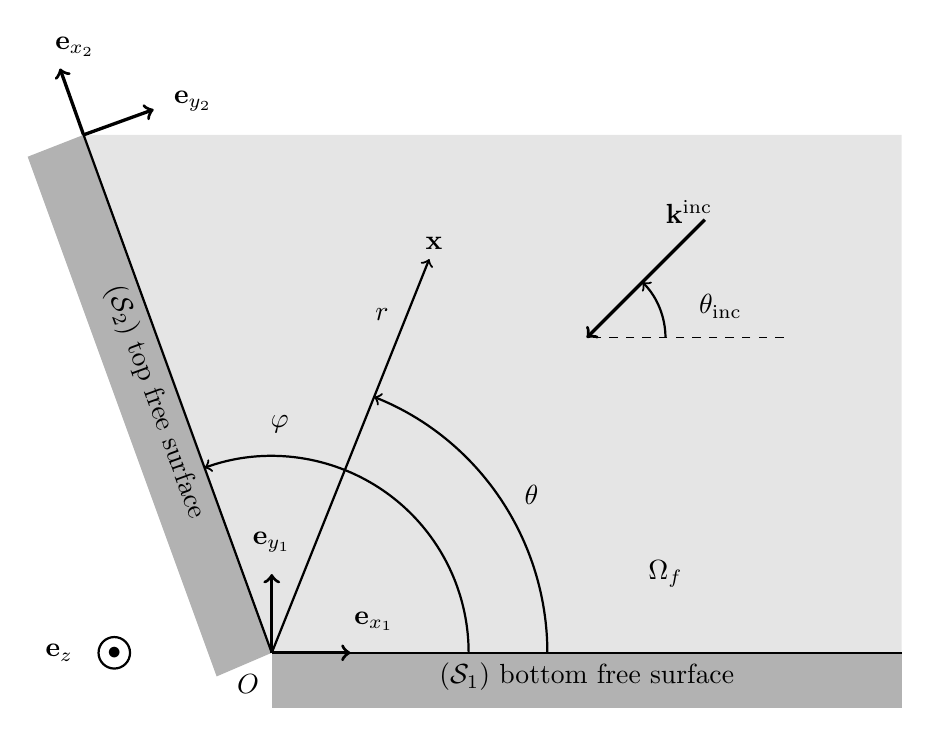
\begin{tikzpicture}
	\fill[color=gray!20] (0,0) -- (8,0)  -- (8,6.5778) -- (-2.39,6.5778) -- cycle;  
	\draw[ thick, ->] (2.5,0) arc (0:110:2.5);
	
	\fill[color=gray!60] (0,0) -- (8,0)  -- (8,-0.7) -- (0,-0.7) -- cycle;  
	
	\fill[color=gray!60] (0,0) --  (-2.39,6.5778) --(-3.1,6.3) -- (-0.7,-0.3) -- cycle; 
		
	\draw[thick, color = black]  (0,0) -- (8,0) node[midway,below] {($\mathcal{S}_1$) bottom free surface};
	
	\draw[thick, color = black]  (0,0) -- (-2.39,6.5778) node[midway,below,sloped] {($\mathcal{S}_2$) top free surface};
	
	\draw[very thick, ->] (-2.39,6.5778) -- (-2.69,7.42);
	
	\node[scale=1] at (-2.5,7.7){$\mathbf{e}_{x_2}$};
	
	\draw[very thick, ->] (-2.39,6.5778) -- (-1.5,6.9);
	
	\node at (-1,7){$\mathbf{e}_{y_2} $};
	
	
	\node at (0.1,2.9){$\varphi$} ; 
	
	\draw[very thick, ->] (0,0) -- (1,0);
	
	\node at (1.3,0.4) {$\mathbf{e}_{x_1} $};
	
	\draw[very thick, ->] (0,0) -- (0,1);
	
	\node at (0,1.4){$\mathbf{e}_{y_1} $};
	
	\node at (-2,-0.01) {$\bullet$};
	
	\draw[thick] (-2,0) circle (0.2);
	
	\node at (-2.7,0){$\mathbf{e}_{z}$};
	
	\draw[very thick, ->] (5.5,5.5) -- (4,4);
	
	\draw[dashed] (6.5,4) -- (4,4);
	
	\draw[thick, ->] (5,4) arc (0:45:1);
	
	\node at (5.7,4.4){$\theta_{\rm inc}$};
	
	\node at (5.3,5.6){ $\mathbf{k}^{\rm inc}$};
	
	\node at (-0.3,-0.4){ $O$};
	
	\node at (5,1){$\Omega_f$ };
	
	% point observation
	
	\draw[thick, ->] (0,0) -- (2,5); 
	
	\draw[thick, ->] (3.5,0) arc (0:68.2:3.5);
	
	\node at (3.3,2){$\theta$};
	
	\node at (1.4,4.3){$r$};
	
	\node at (2.06,5.2){$\mathbf{x}$};
	
	\end{tikzpicture}
	\caption
[Geometry of the problem]
{The wedge of angle $2\varphi$ whose faces are stress-free is illuminated by a plane wave of wave vector $\mathbf{k}^{\rm inc}$.}
\label{chapter5:figure1}
\end{figure}
The dimensionless form of the problem is obtained  by defining the function $h$ by
\begin{equation}
\label{Chapter5:dimensionless}
g(\mathbf{x},t) = 2A \, e^{i \omega t} \, h(k_0 \mathbf{x}).  
\end{equation}

The dimensionless function $h$ is the sum of the  incident dimensionless  wave $h_{inc}$ and of the scattered dimensionless  wave $v$
\begin{equation}
h = h_{inc} + v
\label{decompinc}
\end{equation}
In this decomposition, the scattered wave $v$ is the sum of two fields : the Geometric-Elastodynamic (GE) field, which  is the sum of the possibly multiple specular reflections of the incident wave and of fictitious fields compensating the incident wave in shadow zones, and the diffracted field. A detailed description of the GE field, in the case of a half-plane scatterer, is given by Kamta-Djakou et al. \cite{Audrey}.

The system \eqref{Chapter5:WaveMotion}-\eqref{Chapter5:CL} is equivalent to the following  system of equations for the dimensionless problem, obtained by inserting Fourier transform \eqref{Chapter5:dimensionless} and decomposition \eqref{decompinc} into equations \eqref{Chapter5:WaveMotion} and \eqref{Chapter5:CL}
\begin{equation}
\label{Chapter5:Adimen_waveMotion}
\begin{cases}
(\triangle+1)v =  0 \quad \text{in } \Omega_f, \\
Bv =  -Bh_{inc} \quad \quad \quad \text{on } \mathcal{S}_j, \quad j=1,2
\end{cases}.
\end{equation}

In order to obtain a solution to this problem which is physically relevant, the limiting absorption principle is used. It consists in substituting the wave number $k_0$ by a complex one $k_0 e^{-i\epsilon} $ with $\epsilon > 0$. This means that absorption occurs in the medium and thus the scattered waves attenuate with the distance. The system (\ref{Chapter5:Adimen_waveMotion}) then becomes :
\begin{equation}
\label{Chapter5:waveMotion_epsilon}
(S_\epsilon^*) \quad
\begin{cases}
(\triangle+ \, e^{-2i\epsilon}) v^\epsilon  =  0 \quad \text{in } \Omega_f, \\
Bv^\epsilon  =  -Bh_{\rm inc}^\epsilon  \quad \text{on } \mathcal{S}_j, \quad j=1,2
\end{cases}
\end{equation}

The physically relevant solution to (\ref{Chapter5:Adimen_waveMotion}), called the outgoing solution, can now be defined. It is the one obtained when taking $\epsilon \to 0$ in (\ref{Chapter5:waveMotion_epsilon}). This limit is noted $v^0$. Its integral representation is found hereafter.

\subsection*{Outgoing solution: integral representation}
\label{integral_representation}

First, a special class of distributions is defined.
\begin{definition}
The class of distributions $\mathcal{A}$ is defined as follows. The distribution $f\in \mathcal{A}$ if :
\begin{itemize}
\item $f \in \mathcal{L}^2(\mathbb{R})$ (f is a tempered distribution)
\item supp$(f) \subset \lbrack 0,+\infty \lbrack$
\item $\exists C_0>0$ such that
$$ \sup_{-\pi<\theta<0} \int_{\rho>C_0}|\hat{f}(\rho e^{i\theta})|^2\,d\rho <\infty$$
where $\hat{f}$ is the Fourier transform of $f$ defined by $\hat{f}(\xi)=\int_{\mathbb{R}}f(x)e^{-ix\xi}\, dx$.
\item $\hat{f}(\xi)$ is holomorphic near $\xi=1$
\end{itemize}

\end{definition}
The outgoing solution to (\ref{Chapter5:Adimen_waveMotion}) can now be defined properly.

\begin{definition}
An outgoing solution of the equation (\ref{Chapter5:Adimen_waveMotion}) is a solution v of the form 
\begin{equation}
\label{Chapter5:decomposition}
v=v_1|_{\Omega_f}+v_2|_{\Omega_f}
\end{equation}
where, for $j=1,2$ :
\begin{equation}
\label{inv_potentiels}
v_j=-\lim_{\epsilon \to 0} \left(\Delta+e^{-2i\epsilon}\right)^{-1} \left[ \alpha_j \otimes \delta_{\mathcal{S}_j} \right]
\end{equation}
$\alpha_j \in \mathcal{A}$ are unknown and $\delta_{\mathcal{S}_1}$ and $\delta_{\mathcal{S}_2}$ are the Dirac delta functions on the faces $\mathcal{S}_1$ and $\mathcal{S}_2$ of the wedge respectively (these functions verify $\delta_{\mathcal{S}_j}(x,y)=1$ on $\mathcal{S}_j$, and $\delta_{\mathcal{S}_j}(x,y)=0$ elsewhere).

\end{definition}
The following theorem is proven by Croisille and Lebeau in \cite{CroisilleLebeau} :
\begin{theorem}
The equation \eqref{Chapter5:Adimen_waveMotion} admits a unique outgoing solution.
\end{theorem}

The aim of this chapter is to extend and detail the computation of this outgoing solution for the stress-free wedge immersed in a fluid using the spectral functions method.

The double Fourier transform of a tempered distribution and its inverse are defined by :
\begin{subequations}
\begin{equation}
\hat{f}(\xi,\eta)=\int \int_{\mathbb{R}^2}f(x,y)e^{-i(x\xi+y\eta)}\, {\rm d}x {\rm d}y
\label{fourierdef}
\end{equation}
\begin{equation}
f(x,y)=\frac{1}{4\pi^2}\int\int_{\mathbb{R}^2} \hat{f}(\xi,\eta)e^{i(x\xi+y\eta)}\rm d\xi \rm d\eta
\label{invfourierdef}
\end{equation}
\label{fullfourierdef}
\end{subequations}

The double Fourier transform of (\ref{inv_potentiels}) using \eqref{fourierdef} gives
\begin{equation}
\label{Fourier}
\hat{v_j^\epsilon} =  \left[ \xi^2 + \eta^2 - e^{-2i\epsilon} \right]^{-1} \hat{\alpha_j}.
\end{equation}

 The dimensionless velocity potential $v_j^\epsilon$ is then found by applying the inverse Fourier transform in $\xi$ and $\eta$ to \eqref{Fourier}. 
\begin{equation}
\label{velocity_inv_fourier2}
v_j^\epsilon = \dfrac{1}{4\pi^2}  \int_{-\infty}^{+\infty}\left( \int_{-\infty}^{+\infty} \dfrac{e^{iy_j\eta}}{ \xi^2 + \eta^2 - e^{-2i\epsilon}} {\rm d}\eta \right)\,  \hat{\alpha_j}(\xi) \,  e^{i x_j \xi}  {\rm d} \xi.
\end{equation}

For  $\epsilon \neq 0$, the inner integrand poles are given by
\begin{equation}
 \eta = \pm \sqrt{e^{-2i\epsilon} - \xi^2}  = \pm \zeta_0^\epsilon
\end{equation} 
and are never crossed by integration along the real axis. Integral \eqref{velocity_inv_fourier2} can be calculated using the residue theorem which leads to the following result
\begin{equation}
\label{champ_epsilon}
v_j^\epsilon(x_j,y_j) = \dfrac{i}{4\pi} \int_{-\infty}^{+\infty}  \dfrac{e^{i|y_j|\zeta_0^\epsilon(\xi)} e^{i x_j \xi}}{\zeta_0^\epsilon(\xi)} \hat{\alpha_j}(\xi) \, {\rm d}\xi.
\end{equation}
This integral is well defined if $\text{Im}(\zeta_0^\epsilon) > 0$, so that the exponential in the integral decreases with the distance $y_j$ and the absorption principle is respected. Function $\zeta_0^\epsilon(\xi)$ then satisfies for $\xi$ real
\begin{subequations}
\label{zeta_function}
\begin{align}
\zeta_0^\epsilon(\xi)&= i\sqrt{\xi^2-e^{-i\epsilon}} \quad \text{if} \quad \vert \xi\vert \geq 1,\\
\label{zeta_function_inferior1}
\zeta_0^\epsilon(\xi)&= -\sqrt{e^{-i\epsilon}-\xi^2} \quad  \text{if} \quad \vert \xi\vert \leq 1.
\end{align}
\end{subequations}
The branch points of the function $\zeta_0^\epsilon(\xi)$ are $\pm  \, e^{-i\epsilon}$. For $\epsilon > 0$, integral \eqref{champ_epsilon} is well defined because these complex singular points are never crossed by the integration contour (the real axis). The integration contour of \eqref{champ_epsilon}, is deformed into the contour $\Gamma_0$ illustrated on Fig.~\ref{chapter5:figure2} so that these singular points $\pm  \, e^{-i\epsilon}$ are not crossed by the new contour $\Gamma_0$  when $\epsilon \rightarrow 0$ (for which the physical outgoing solution of (\ref{Chapter5:waveMotion_epsilon}) is obtained). The curved arrows on Fig.~\ref{chapter5:figure2} are described later in section \ref{Chapter5:regular_part}.

Thus, even for $\epsilon=0$, the integral
\begin{equation}
\label{champ}
v_j^0(x_j,y_j) = \dfrac{i}{4\pi} \int_{\Gamma_0}  \dfrac{e^{i|y_j|\zeta_0^0(\xi)} e^{i x_j \xi}}{\zeta_0^0(\xi)} \hat{\alpha_j}(\xi)  \, {\rm d}\xi
\end{equation}
converges.
Using \eqref{Chapter5:decomposition}, our initial solution is then
\begin{equation}
\label{initial_sol}
v(\mathbf{x}) = v_1^0(x_1,y_1) + v_2^0(x_2,y_2)
\end{equation}

\begin{figure}[ht]%
	\centering
	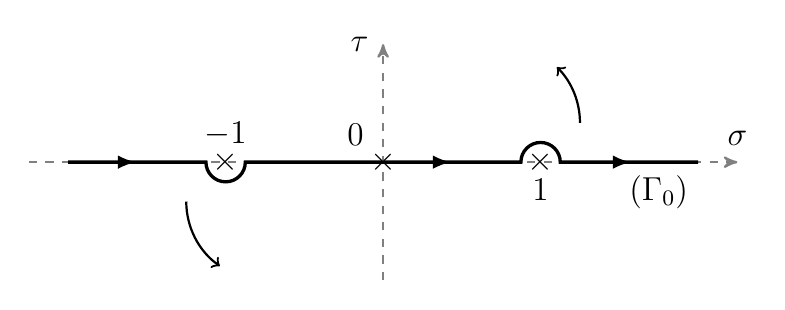
\begin{tikzpicture}
	\node at (0,0) {\large $\times$};
	\node at (-0.35,0.35) {\large $0$};
	\node at (2,0) {\large $\times$}; % Pole
	\node at (2,-0.35) {\large $1$};
	\node at (-2,0) {\large $\times$};
	\node at (-2,0.35) {\large $-1$}; %pole
	\node at (3.5,-0.38) {\large $(\Gamma_0)$};
	\draw[ thick, ->] (-2.5,-0.5) arc (180:235:1);
%	\node at (-2.8,-0.9) {\large $\mathcal{F}_1$};
	\draw[ thick, ->] (2.5,0.5) arc (0:45:1); %ici c'est les fleches 
	%\node at (2.8,0.9) {\large $\mathcal{F}_2$};
    \node at (4.5,0.3) {\large $\sigma$};
    \node at (-0.3,1.5) {\large $\tau$};
	\draw[step=1.5cm,gray,thick,dashed,->,>=stealth'] (-4.5,0) -- (4.5,0);
	\draw[step=1.5cm,gray,thick,dashed,->,>=stealth'] (0,-1.5) -- (0,1.5);
	\draw[very thick,black,yshift=0pt,
	decoration={ markings,  % This schema allows for fine-tuning the positions of arrows 
		mark=at position 0.1 with {\arrow{latex}},
		mark=at position 0.6 with {\arrow{latex}},
		mark=at position 0.9 with {\arrow{latex}}},
	postaction={decorate}]
	(-4,0)  -- (-2.25,0)  arc (-180:0:0.25)  -- (1.75,0)arc (180:0:0.25)  --  (4,0); % ca c'est l'axe
	\end{tikzpicture}
\caption
[Contour $\Gamma_0$]
{Integration contour $\Gamma_0$ in the complex plane $\xi = \sigma + i \tau$. The curved arrows show the deformation of $\Gamma_0$ into the imaginary axis.}
\label{chapter5:figure2}
\end{figure}

One of the goals of this chapter is to compute the spectral functions $\hat{\alpha}_1(\xi)$ and $\hat{\alpha}_2(\xi)$ in order to find the GTD diffraction coefficient \eqref{GTDCoeff_SF}. The accuracy of the spectral functions method is evaluated in section 4 by comparing results of \eqref{GTDCoeff_SF} with \eqref{GTDCoeff_Dir} in the case of Dirichlet boundary conditions and \eqref{GTDCoeff_Neu} in the case of Neumann boundary conditions. Section \ref{Chapter5:resolution} is devoted to the computation of the spectral functions $\hat{\alpha}_1$ and $\hat{\alpha}_2$.


\section{Spectral functions computation}
\label{Chapter5:resolution}

To compute the spectral functions, the functional equations satisfied by these spectral functions $\hat{\alpha}_1$ and $\hat{\alpha}_2$ first have to be determined.
\subsection{Functional equations of spectral functions}

The velocity potential in the boundary conditions of the system \eqref{Chapter5:waveMotion_epsilon} is substituted by its expression \eqref{initial_sol}. It then leads to the following system of equations for the boundary conditions on each wedge face:
\begin{equation}
\label{CL}
\begin{cases}
Bv_1^0(x_1,0) + Bv_2^0(x_2 \cos \varphi,x_2 \sin \varphi)  =  -Bv^0_{\rm inc} \mid_{\mathcal{S}_1}\\
Bv_1^0(x_1 \cos \varphi,x_1 \sin \varphi) + Bv_2^0(x_2,0)   =  -Bv^0_{\rm inc} \mid_{\mathcal{S}_2}
\end{cases}.
\end{equation}
The Fourier transform is applied to the potential velocity expression on the face of each wedge
\begin{align}
\mathcal{F}(x_j \mapsto v_j^0 (x_j,0))(\xi) & =  \dfrac{i}{4\pi} \int_{\Gamma_0}  \dfrac{\hat{\alpha_j}(\lambda)}{\zeta_0^0(\lambda)}  \left( \int_0^{\infty} \, e^{-i x_j (\xi-\lambda)} dx_j \right) {\rm d} \lambda,\\
& =  \dfrac{1}{4\pi} \int_{\Gamma_0} \dfrac{\hat{\alpha_j}(\lambda)}{\zeta_0^0(\lambda) (\xi - \lambda)} {\rm d} \lambda \nonumber
\end{align}
and
\begin{align}
\mathcal{F} \left( x_j \mapsto v_j^0 \left( x_j \cos \varphi,x_j \sin \varphi \right) \right)(\xi)  & =  \dfrac{i}{4\pi} \int_{\Gamma_0}  \dfrac{\hat{\alpha_j}(\lambda)}{\zeta_0^0(\lambda)}  \left( \int_0^{\infty} \, e^{-i x_j \left( \xi - \lambda  \, \cos \varphi - |\sin \varphi| \, \zeta_0^0(\lambda) \right)} dx_j \right) {\rm d} \lambda,\\
& = \dfrac{1}{4\pi} \int_{\Gamma_0} \dfrac{ \hat{\alpha_j}(\lambda)}{\zeta_0^0(\lambda) \left[ \xi - \lambda \, \cos \varphi  - |\sin \varphi| \, \zeta_0^0(\lambda) \right]} {\rm d} \lambda.  \nonumber
\end{align}
The potential velocity's normal derivative on the face of each wedge is computed using \eqref{champ}, and by noting that for each face $n_j=y_j$ (see Fig.~\ref{chapter5:figure1}) :
\begin{equation}
\frac{\partial v_j^0}{\partial n_j}(x_j,y_j) = -\frac{1}{4\pi} \int_{\Gamma_0} te^{i\xi x_j}e^{i|y_j|\zeta_0^0(\xi)} \hat{\alpha_j}(\xi)\, d\xi,
\end{equation}
where $t= \rm sgn \, y_j$. In order to go from one Cartesian coordinate system to another, the following change in variables is given for $j=1,2$ (see Fig.~\ref{chapter5:figure1}) :
\begin{eqnarray}
\label{changecoords}
\left\{
\begin{array}{l}
x_{3-j}=x_j\cos\varphi+y_j\sin\varphi \\
y_{3-j}=x_j\sin\varphi-y_j\cos\varphi
\end{array}
\right.
\end{eqnarray}
This yields :
\begin{align}
\frac{\partial v_j^0}{\partial n_{3-j}}&=\frac{\partial v_j^0}{\partial y_{3-j}}= \sin\varphi \frac{\partial v_j^0}{\partial x_j}-\cos\varphi \frac{\partial v_j^0}{\partial y_j}\\
&=-\frac{1}{4\pi}\int_{\Gamma_0}\frac{(\xi\sin\varphi-t\cos\varphi\zeta_0^0(\xi))}{\zeta_0^0(\xi)}e^{i(\xi x_j+|y_j|\zeta_0^0(\xi))}\hat{\alpha_j}(\xi)\,d\xi
\end{align}
The Fourier transform can now also be applied to the potential velocity's normal derivative on the each face of the wedge
\begin{align}
\mathcal{F}(x_j \mapsto \frac{\partial v_j^0}{\partial n_j} (x_j,0))(\xi)&=-\frac{1}{4\pi} \int_{\Gamma_0}  \hat{\alpha_j}(\lambda)\left( \int_0^{\infty} \, e^{-i x_j (\xi-\lambda)} dx_j \right)\, d \lambda \nonumber\\
&=\frac{i}{4\pi}\int_{\Gamma_0}\frac{\hat{\alpha_j}}{\xi-\lambda}\, d\lambda
\end{align}
and
\begin{align}
\mathcal{F} &\left( x_j \mapsto \frac{\partial v_j^0}{\partial n_{3-j}} ( x_j \cos \varphi,x_j \sin \varphi) \right)(\xi)  \nonumber\\
& =  -\frac{1}{4\pi} \int_{\Gamma_0}  \frac{(\lambda\sin\varphi-t\cos\varphi\zeta_0^0(\lambda))}{\zeta_0^0(\lambda)}\hat{\alpha_j}(\lambda)  \left( \int_0^{\infty} \, e^{-i x_j \left( \xi - \lambda  \, \cos \varphi - |\sin \varphi| \, \zeta_0^0(\lambda) \right)} dx_j \right) \,d \lambda, \nonumber\\
& = \frac{i}{4\pi} \int_{\Gamma_0} \dfrac{ \lbrack \lambda\sin\varphi-t\cos\varphi\zeta_0^0(\lambda)\rbrack \, \hat{\alpha_j}(\lambda)}{\zeta_0^0(\lambda) \left[ \xi - \lambda \, \cos \varphi  - |\sin \varphi| \, \zeta_0^0(\lambda) \right]} \, d\lambda,
\end{align}
here $t=\rm sgn \sin \varphi$.

The dimensionless incident wave on the faces $\mathcal{S}_1$ and $\mathcal{S}_2$ of the wedge which is involved at the right side of \eqref{CL} is respectively:
\begin{subequations}
\label{CL2}
\begin{align}
v^0_{\rm inc}(x_1,y_1) & =  \dfrac{1}{2} \, e^{i \, (x_1 \cos \theta_{inc}+y_1\sin\theta_{inc} ) } ,\\
v^0_{\rm inc}(x_2,y_2) & =   \dfrac{1}{2} \, e^{i \, (x_2 \cos (\varphi - \theta_{inc} )+y_2\sin(\varphi-\theta_{inc}))} 
\end{align}
\end{subequations}

Therefore, applying the Fourier transform to \eqref{CL} leads to the following functional system of equations:
\begin{equation}
\label{functional_eq}
\begin{cases}
DM(\hat{\alpha}_1)(\xi) + TM(\hat{\alpha}_2)(\xi) = \dfrac{W_1}{\xi - Z_1} \\
TM(\hat{\alpha}_1)(\xi) + DM(\hat{\alpha}_2)(\xi)  = \dfrac{W_2}{\xi - Z_2} 
\end{cases}
\end{equation}
where $Z_1 =  \cos \theta_{\rm inc}$, $Z_2 =  \cos (\varphi - \theta_{\rm inc})$, $W_1=W_2=1$ in the case of Dirichlet boundary conditions and $W_1=\sin\theta_{inc}, \quad W_2=\sin(\varphi-\theta_{inc})$ in the case of Neumann boundary conditions. $DM$ is an integral operator defined as
\begin{equation}
\label{DM_operator}
\begin{split}
DM(\hat{\alpha}_1)(\xi) = \int_{\Gamma_0} DM(\xi,\lambda) \, \hat{\alpha}_1(\lambda) \, d \lambda =\dfrac{1}{2i\pi} \int_{\Gamma_0} \dfrac{dm(\lambda)  }{\xi - \lambda} \hat{\alpha}_1(\lambda) \, d\lambda
\end{split}
\end{equation}
where 
\begin{equation}
\label{dmDir}
dm(\lambda) = \dfrac{1}{\zeta_0^0(\lambda)}
\end{equation}
in the case of Dirichlet boundary conditions and 
\begin{equation}
\label{dmNeu}
dm(\lambda)=1
\end{equation}
in the case of Neumann boundary conditions. 

$TM$ is an integral operator defined as
\begin{equation}
\label{TM_operator}
\begin{split}
TM(\hat{\alpha}_1)(\xi) &= \int_{\Gamma_0} TM(\xi,\lambda) \, \hat{\alpha}_1(\lambda) \, {\rm d} \lambda =\dfrac{1}{2i\pi} \int_{\Gamma_0} \dfrac{ tm(\lambda)}{ \xi- \lambda \cos \varphi  - |\sin \varphi| \zeta_0^0(\lambda)} \hat{\alpha}_1(\lambda) \, {\rm d} \lambda 
\end{split}
\end{equation}
where 
\begin{equation}
\label{tmDir}
tm(\lambda)=\dfrac{1}{\zeta_0^0(\lambda)}
\end{equation}
in the case of Dirichlet boundary conditions and 
\begin{equation}
\label{tmNeu}
tm(\lambda)=\dfrac{\lambda\sin\varphi-t\cos\varphi\zeta_0^0(\lambda)}{\zeta_0^0(\lambda)}
\end{equation}
in the case of Neumann boundary conditions.
Note that the function $TM$ can be expressed as
\begin{equation}
TM(\xi,\lambda) =  \dfrac{1}{2i\pi} \dfrac{ tm(\lambda)}{ \xi- T_0(\lambda)} , 
\end{equation}
where, applying the variable change $\lambda=\cos\theta$
\begin{equation}
\label{Trans_operator}
T_0(\lambda=\cos\theta) =  \lambda \cos \phiti  + \sin \phiti \, \zeta_0^0(\lambda) =  \cos (\theta + \phiti)
\end{equation}
with 
\begin{equation}
\phiti =
\begin{cases}
 \varphi \quad \text{if} \quad 0 < \varphi < \pi \qquad \\
 2\pi - \varphi \quad \text{if} \quad \pi < \varphi < 2\pi
 \label{phitilde}
\end{cases}
\end{equation}
Function $T_0$ is therefore called the translation operator, since it translates the complex angle $\theta$ to $\theta+\phiti$. By using this angular variable, defined differently for wedge angles lower and higher than $\pi$, the description of the spectral functions method can be written the same way for wedge angles lower and higher than $\pi$, even if the final results (the diffraction coefficients) are different for wedge angles $\pi<\varphi<2\pi$ and $2\pi-\varphi$. Indeed, the variable $\varphi$ appears in all the resolution, whereas the variable $\phiti$ appears only in the definition of the function $T_0$ in \eqref{Trans_operator} and of the domain $\Omega_0$ in which $T_0$ operates, defined as
\begin{equation}
\label{Domain_Omega0}
\Omega_0 =\{\xi\in\mathbb C, \ \xi=\cos \theta, \ 0< {\rm Re } \, \theta < \pi -\phiti \}.
\end{equation}
Domain $\Omega_0$ is delineated by the hyperbola 
\begin{equation}
\partial \Omega_0^+ = \{   \xi \in \mathbb{C}, \quad \xi = \cos \theta, \quad {\rm Re}  \theta = \pi - \phiti \}.
\end{equation}
Domain $\Omega_0$ and its upper boundary $\partial \Omega_0^+$ are illustrated on Fig.~\ref{chapter5:figure4}. Domain $\Omega_0$ is the grey area in Fig.~\ref{chapter5:figure4}.

\begin{figure}[h]
\centering
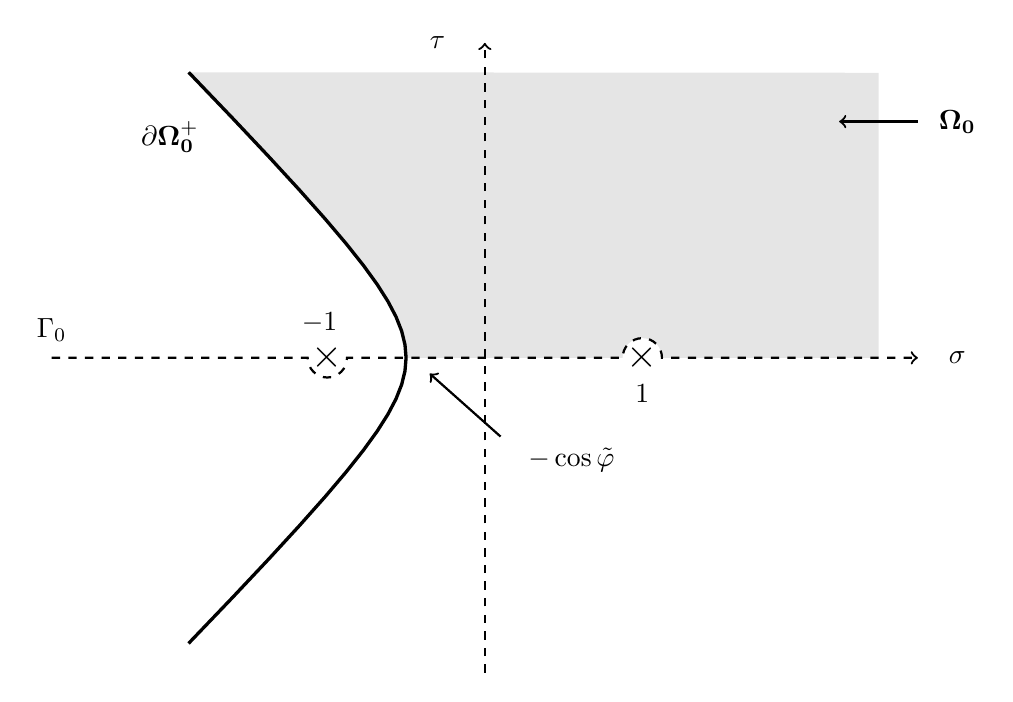
\begin{tikzpicture}
% Filling Omega_0
\fill [color=gray!20]
(5,0)
-- plot [domain=0:2] ({-cosh(\x)},{sinh(\x)})
-- (5,3.62)
-- cycle;

\fill[color=white] (2,0) circle (0.25);

\node at (2,0) {\Large $\mathbf{\times}$}; % Pole
\node at (2,-0.45) { $1$};
\node at (-2,0) {\Large $\mathbf{\times}$};
\node at (-2.1,0.45) {$-1$}; %pole
\node at (-5.5,0.35) {$\Gamma_0$};
\draw[dashed,thick, ->]
      (-5.5,0) -- (-2.25,0)  arc (-180:0:0.25)  -- (1.75,0)arc (180:0:0.25) -- (5.5,0);
\draw[dashed,thick,->]
	  (0,-4) -- (0,4);
\node at (6,0) {$\sigma$};
\node at (-0.6,4) { $\tau$};
      % axis

%% arrows indicating countour deformation
%\draw[ thick, ->] (-3,-0.25) arc (180:235:1);
%\node at (-3.2,-0.9) {$\mathcal{F}_1$};
%\draw[ thick, ->] (4.0,0.3) arc (0:45:1); 
%\node at (4.5,0.8) { $\mathcal{F}_2$};

% Hyperbola (contour  partial_Omega_0 )
\draw[black, very thick][domain=-2:2] plot({-cosh(\x)}, {sinh(\x)});
\node at (-4.0,2.8) { $\mathbf{\partial \Omega_0^+}$};
\draw[thick,->] (0.2,-1.0)--(-0.7,-0.2);
\node at (1.1,-1.3) {$-\cos \phiti$};

%  Omega_0
\draw [thick, ->] (5.5,3)--(4.5,3);
\node at (6,3) {$\mathbf{\Omega_0}$};

\end{tikzpicture}
\caption
[Contour $\partial \Omega_0^+$]
{Domain $\Omega_0$ (the grey area) and its upper boundary $\partial \Omega_0^+$. The lower boundary of $\Omega_0$ is the semi-axis $[-\cos \phiti,+\infty[$.}
\label{chapter5:figure4}
\end{figure}
Having found the system of functional equations, it is now resolved following the methodology of Croisille and Lebeau \cite{CroisilleLebeau}.

\subsection{System resolution}
\label{Chapter5:System_resolution}

The resolution of the system of functional equations \eqref{functional_eq} is necessary in order to find the values of the spectral functions $\hat{\alpha}_1 $ and $\hat{\alpha}_2 $. With these values, the diffraction coefficients can be computed using equation \eqref{GTDCoeff_SF}. 

It is shown in \cite{CroisilleLebeau} that $DM$ and $TM$ integral operators are constituted of a "singular term" and of a "regular term". For a singular function 
\begin{equation}
\label{Chapter5:arbitrary_function}
\phi(\xi) = \dfrac{1}{\xi - z},  \quad z \in \mathbb{C}\setminus ]-\infty,-1] \text{ with } {\rm Im} \, z \geqslant 0,
\end{equation}
$DM$ and $TM$ integral operators defined respectively in \eqref{DM_operator} and \eqref{TM_operator} can be decomposed using the residue theorem as
\begin{subequations}
\label{Int_op_decomp}
\begin{align}
\label{Int_op_decomp_DM}
DM(\phi)(\xi) &= \int_{\Gamma_0} DM(\xi,\lambda) \cdot \dfrac{1}{\lambda - z} \, d \lambda = \dfrac{dm(z)}{\xi - z}  + D_p(\xi,z) \\
\label{Int_op_decomp_TM}
TM(\phi)(\xi) &= \int_{\Gamma_0} TM(\xi,\lambda) \cdot \dfrac{1}{\lambda - z} \, d \lambda = \dfrac{tm(z) }{\xi - T_0(z)} 1_{\Omega_0}(z) + T_p(\xi,z),
\end{align}
\end{subequations}
where the function $T_0$ is defined in \eqref{Trans_operator} and where
\begin{equation}
1_{\Omega_0}(z) = 
\begin{cases}
1 \quad \text{if } z  \in \Omega_0, \\
0 \quad \text{else}
\end{cases}
\end{equation}
and integrals $D_p$ and $T_p$ are holomorphic on $\mathbb{C}\setminus ]-\infty,-1]$. Such integrals are expressed as
\begin{subequations}
\label{holomorphic_functions}
\begin{align}
\label{defDp}
D_p(\xi,z) &= \dfrac{1}{2\pi i}\int_{\Gamma_1} \dfrac{dm(\lambda)}{\xi-\lambda} \cdot \dfrac{1}{\lambda - z} d\lambda, \\
\label{defTp}
T_p(\xi,z) &= \dfrac{1}{2\pi i}\int_{\partial \Omega_0^+}  \dfrac{tm(\lambda)}{\xi-T_0(\lambda)} \cdot \dfrac{1}{\lambda - z} d\lambda.
\end{align}
\end{subequations}
Contours $\Gamma_1$ and $\partial \Omega_0^+$ are illustrated on Figs.~\ref{chapter5:figure5} and \ref{chapter5:figure4} respectively.

\begin{figure}[ht]
\centering
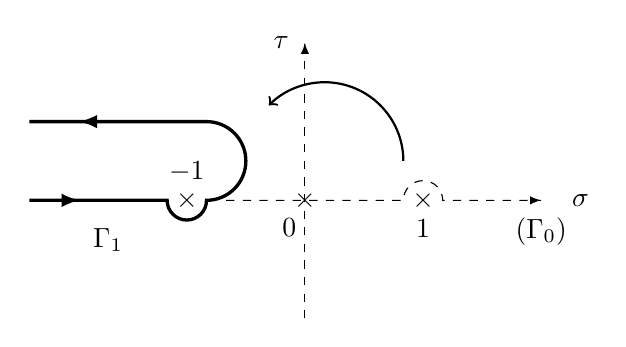
\begin{tikzpicture}
\node at (-0.5,0) {  $\times$};
\node at (-0.7,-0.35) { $0$};
\node at (1,0) { $\times$}; % Pole
\node at (1,-0.36) { $1$};

\node at (-2,0) { $\times$};
\node at (-2,0.36) {  $-1$}; %pole
\node at (-3,-0.5) { $\Gamma_1$};

\draw[dashed, decoration={markings,
 mark=at position 1.0 with {\arrow{latex}}},
      postaction={decorate}] (-1.5,0) -- (0.75,0) arc (180:0:0.25)-- (2.5,0);
\node at (3,0) {$\sigma$};
\draw[dashed, decoration={markings,
 mark=at position 1.0 with {\arrow{latex}}},
      postaction={decorate}] (-0.5,-1.5) -- (-0.5,2);
\node at (-0.8,2) {$\tau$};      

\node at (2.5,-0.4) {$(\Gamma_0)$};
      
\draw[ thick, ->] (0.75,0.5) arc (0:135:1); 
  

\draw[very thick, black, yshift=0pt,
decoration={ markings,  % This schema allows for fine-tuning the positions of arrows 
      mark=at position 0.1 with {\arrow{latex}},
      mark=at position 0.9 with {\arrow{latex}}},
      postaction={decorate}]
      (-4,0) -- (-2.25,0)  arc (-180:0:0.25) -- (-1.75,0) arc(-90:90:0.5)  -- (-4,1);
\end{tikzpicture}
\caption
[Contour $\Gamma_1$]
{Contour $\Gamma_1$. The curved arrow shows the deformation of $\Gamma_0$ (dashed line) into $\Gamma_1$.}
\label{chapter5:figure5}
\end{figure}

In the sequel, using the decomposition of the $DM$ and $TM$ operators for a function of the form of \eqref{Chapter5:arbitrary_function}, it will be shown that the unknown spectral functions $\hat{\alpha}_1$ and $\hat{\alpha}_2$ in the system \eqref{functional_eq} have a singular part. The first step for the resolution of the system \eqref{functional_eq} is then to determine this singular part.

\subsubsection{Singular part}
\label{Chapter5:sing_part}

It is well known that poles of the spectral functions lead to the reflections of the incident field on the wedge faces (these reflections can be multiple), and to the fictitious fields that compensate the incident wave in the shadow zones. The sum of these reflections with the fictitious compensating fields constitute the aforementioned GE field. The singular part of the spectral functions contains these poles. The goal of this subsection is to calculate the poles and the corresponding residues and then to determine the expression of the singular part of the spectral functions, by employing a recursive algorithm. 

Knowing the incident field on the wedge faces, the spectral function  $\hat{\alpha}_j$ can be written as
\begin{equation}
\label{Chapter5:ini_pol_propag}
\hat{\alpha}_j(\xi) = \dfrac{V_j}{\xi - Z_j} + X_j'(\xi), \quad j=1,2
\end{equation}
where $Z_1,Z_2$ are the initial poles, given in (\ref{functional_eq}) with unknown residues $V_1$ and $V_2$ and the functions $X_j'$ are unknown, $j=1,2$. From \eqref{Int_op_decomp_DM}, it is known that
\begin{equation}
\label{Chapter5:pole_propag_DM_1}
DM(\hat{\alpha}_j)(\xi) = \dfrac{dm(Z_j) \cdot V_j}{\xi - Z_j} + D_p(\xi,Z_j)\cdot V_j + DM( X_j')(\xi).
\end{equation}
By choosing $V_j =  dm^{-1}(Z_j).W_j$, the right hand side of the system \eqref{functional_eq} is suppressed by the first term in the right hand side of \eqref{Chapter5:pole_propag_DM_1}. The resulting system's unknown functions are $X'_j, \, j=1,2$ :
\begin{equation}
DM  (X_j' )(\xi)+ TM (X_{3-j}' )(\xi) = - TM  \left(  \dfrac{V_{3-j}}{\xi - Z_{3-j}} \right) (\xi)  - D_p(V_j,Z_j)(\xi) \qquad j=1,2
\end{equation}
Applying \eqref{Int_op_decomp_TM} yields
\begin{equation}
\label{Chapter5:pol_propag_step3}
TM  \left(  \dfrac{V_j}{\xi - Z_j} \right)(\xi) = \dfrac{tm(Z_j) \cdot V_j}{\xi - T_0(Z_j)}  \, 1_{\Omega_0}(Z_j) + T_p(\xi,Z_j)\cdot V_j \qquad j=1,2
\end{equation}
Thus, $X_j'$ has a pole at $\xi = Z_j^{1)} = T_0(Z_{3-j})$ if $Z_{3-j} \in \Omega_0$. The wave incident on face $\mathcal{S}_{3-j}$ is reflected. This reflected wave is incident on face $\mathcal{S}_j$, generating a new pole $Z_j^{(1)}=T_0(Z_{3-j})$. 
The unknown function $X_j'$ in \eqref{Chapter5:ini_pol_propag} is then decomposed as
\begin{equation}
\label{Chapter5:pol_propag_step2}
X_j'(\xi) =  \dfrac{V_j^{(1)}}{\xi - Z_j^{(1)}} + X_j''(\xi), \quad j=1,2
\end{equation}
where the function $ X_j''$ is unknown. 
Once again, the residues $V_j^{(1)}$ of these generated poles $Z_j^{(1)}$ are chosen so that they cancel the singular term in $DM(X_j')(\xi)$, found using formula \eqref{Int_op_decomp_DM}, compensating the singular term in the $TM$ operator in \eqref{Chapter5:pol_propag_step3}.

This pole propagation process is applied recursively in order to determine all the poles of the spectral functions $\hat{\alpha}_j$. This process stops when the generated poles are no longer in the domain $\Omega_0$ defined in \eqref{Domain_Omega0}. All the generated poles then belong to $\Omega_0$. 

At the end of this process, the spectral functions have the following decomposition
\begin{equation}
\label{spec_decomp}
\hat{\alpha}_j=Y_j+X_j, 
\end{equation}
where  $Y_j$ is the singular part, $X_j$ is the regular part  and $j=1,2$ is the face index. The singular part is expressed as
\begin{equation}
\label{sing_part}
 Y_j(\xi) = \sum_i {V_j^{(i)} \over \xi - Z_j^{(i)}},
\end{equation}
where $i \in \mathbb{N}^*$, $Z_j^{(0)} = Z_j$ defined in \eqref{functional_eq} is the initial pole on each face of the wedge, $V_j^{(0)}=V_j$ is the corresponding initial residue on each face of the wedge, 
\begin{equation}
\label{Generated_poles}
Z_j^{(i+1)} = T_0(Z_{3-j}^{(i)}) \quad j=1,2
\end{equation} 
are the different generated poles with their respective residues 
\begin{equation}
\label{Generated_residues}
V_j^{(i+1)}=-dm^{-1}(T_0(Z_{3-j}^{(i)})) \,  tm(Z_{3-j}^{(i)})) \, V_{3-j}^{(i)} \, 1_{\Omega_0}(Z_{3-j}^{(i)}), \quad  j=1,2.
\end{equation}
\paragraph{}
Figure \ref{poles} represents the generated poles in the complex plane for two different cases : figure \ref{poles80} for a wedge of angle $\varphi=80^o$ with an incident angle of $\theta_{inc}=55^o$ and figure \ref{poles20} for $\varphi=20^o$ and $\theta_{inc}=15^o$. As the wedge angle decreases, the number of poles increases, some poles being very close to one another, rendering the method less accurate for very small wedge angles.
\begin{figure}[h]
	\centering
	\begin{subfigure}[b]{0.4\textwidth}
	\begin{tikzpicture}[scale=2]
	\draw[->,>=stealth'] (-1.25,0) -- (1.25,0);
	\draw[->,>=stealth'] (0,-0.5) -- (0,0.5);
	\node at (1.25,0)[right]{Re};
	\node at (0,0.5)[right]{Im};
	
	\node at (-1,0){$\bullet$};
	\node at (1,0){$\bullet$};
	\draw (-1,0) node[below] {$-1$};
	\draw (1,0) node[below] {$1$};
	
	\node at ( 0.573576450    ,  0.00000000    ){$\times$};
	\node at ( 0.906307757    ,  0.00000000    ){$\times$};
	\node at (-0.258819222    ,  0.00000000    ){$\times$};
	\node at (-0.707106829    ,  0.00000000    ){$\times$};
	\end{tikzpicture}
	\subcaption{$\varphi=80^o, \, \theta_{inc}=55^o$}
    \label{poles80}
	\end{subfigure}
\hspace{1em}
\begin{subfigure}[b]{0.4\textwidth}
\begin{tikzpicture}[scale=2]
\draw[->,>=stealth'] (-1.25,0) -- (1.25,0);
\draw[->,>=stealth'] (0,-0.5) -- (0,0.5);
\node at (1.25,0)[right]{Re};
\node at (0,0.5)[right]{Im};

\node at ( 0.965925813    ,  0.00000000    ){$\times$};
\node at ( 0.996194720    ,  0.00000000    ){$\times$};
\node at ( 0.906307876    ,  0.00000000    ){$\times$};
\node at ( 0.819151998    ,  0.00000000    ){$\times$};
\node at ( 0.573576331    ,  0.00000000    ){$\times$};
\node at ( 0.707106948    ,  0.00000000    ){$\times$};
\node at ( 0.422618449    ,  0.00000000    ){$\times$};
\node at ( 0.258818895    ,  0.00000000    ){$\times$};
\node at ( -8.71558934E-02,  0.00000000    ){$\times$};
\node at (  8.71559381E-02,  0.00000000    ){$\times$};

\node at (-1,0){$\bullet$};
\node at (1,0){$\bullet$};
\draw (-1,0) node[below] {$-1$};
\draw (1,0) node[below] {$1$};
\end{tikzpicture}
\subcaption{$\varphi=20^o, \, \theta_{inc}=15^o$}
\label{poles20}
\end{subfigure}
\caption{Poles generated by the recursive algorithm plotted in the complex plane}
\label{poles}
\end{figure}

The second step of the system resolution is the determination of the regular part $X_j$ of the spectral function $\hat{\alpha}_j$, see Eq.~\eqref{spec_decomp}. The regular part is determined by using the Galerkin collocation method. Section \ref{Chapter5:regular_part} gives the principal steps of this resolution method. 

\subsubsection{Regular part}
\label{Chapter5:regular_part}

After the determination of the singular part of the solution using the pole propagation process explained in section \ref{Chapter5:sing_part}, the remaining system \ref{functional_eq} is by construction
\begin{equation}
\label{sys_regular}
\begin{cases}
DM(X_1)(\xi) + TM(X_2)(\xi) = -\underset{k}{\sum} \Big( D_p(\xi,Z_1^{(k)})\cdot V_1^{(k)}+ T_p(\xi,Z_2^{(k)})\cdot V_2^{(k)}\Big)\\
TM(X_1)(\xi) + DM(X_2)(\xi)  =  -\underset{k}{\sum} \Big( T_p(\xi,Z_1^{(k)})\cdot V_1^{(k)}+ D_p(\xi,Z_2^{(k)})\cdot V_2^{(k)}\Big)
\end{cases}
\end{equation}
where $X_j$, $j=1,2$ are the regular parts of the spectral functions \eqref{spec_decomp}, $D_p$ and $T_p$ functions are defined in \eqref{holomorphic_functions} and $Z_j^{(k)}$ are the poles of spectral function $\hat{\alpha}_j$  and their respective residues are $V_j^{(k)}$. According to Croisille and Lebeau \cite{CroisilleLebeau}, $D_p$ and $T_p$ are holomorphic on $\mathbb{C}\setminus  ]-\infty,-1]$ and therefore functions $X_1$ and $X_2$ are also holomorphic on this domain.

The functions $X_j(\xi)$, being holomorphic on $\mathbb{C}\setminus  ]-\infty,-1]$, can be approached in the vectorial subspace generated by $\varphi_k, \, 1 \leq k \leq N$ where
\begin{equation}
\label{Gal_basis}
\varphi_k(\xi) = \dfrac{d_k}{\xi + a_k}, \quad a_k \in [1,\infty[, \quad d_k=\sqrt{\frac{a_k}{\pi}}.
\end{equation}
The approximation of the solution $X_j(\xi)$ in this subspace of finite dimension is called a Galerkin approximation.

In the following, the integration contour $\Gamma_0$ pictured on Fig.~\ref{chapter5:figure2} is deformed into the imaginary axis. If $f(\lambda)$ is a holomorphic function on $\mathbb{C}\setminus  ]-\infty,-1]$, the function $\tilde f (y)=f(iy)$ is introduced so that $\tilde f$ is holomorphic on $\mathbb{C}\setminus i [1,\infty[ $. The variable change $\lambda = iy$ gives a new basis
\begin{equation}
\label{Galerkin_basis}
e_{a_k}(y) = \dfrac{d_k}{y-i{a_k}}=i\tilde \varphi(y), \quad \text{with} \quad d_k=\sqrt{\frac{a_k}{\pi}} \quad \text{and} \quad a_k \in [1,\infty[,
\end{equation}

Having an approximation basis of the regular part of the spectral functions, $X_j(\xi)$ can be expressed as
\begin{equation}
\label{regular_part_decomp}
X_j(\xi) \approx \sum_{k=1}^N \tilde{X}_j^k \, \varphi_k(\xi), \quad \tilde{X}_j^k \in \mathbb{C}.
\end{equation}
The coordinates $\tilde{X}_j^k$ are unknown. The system \eqref{sys_regular} then becomes, for $j=1,2$
\begin{equation}
\label{sys_regular_gal}
\sum_{k=1}^N \left[ \tilde{X}_j^k \, \int_{\Gamma_0} DM(\xi,\lambda) \varphi_k(\lambda) \, {\rm d} \lambda + \tilde{X}_{3-j}^k \, \int_{\Gamma_0} TM(\xi,\lambda) \varphi_k(\lambda) \, {\rm d} \lambda \right] = u_j(\xi), 
\end{equation}
where
\begin{equation}
\label{second_member}
u_j(\xi) = -\sum_k \Big( D_p(\xi,Z_j^k)\cdot V_j^k+ T_p(\xi,Z_{3-j}^k)\cdot V_{3-j}^k\Big) \qquad j=1,2
\end{equation}
The variable changes $\lambda = iy$ and $\xi = ix$ in \eqref{sys_regular_gal} lead to the following system $(j=1,2)$
\begin{equation}
\label{sys_regular_gal_def}
\sum_{k=1}^N \left[ \tilde{X}_j^k \, \int_{-\infty}^\infty  \widetilde{DM}(x,iy) \, e_{a_k}(y) {\rm d} y + \tilde{X}_{3-j}^k \, \int_{-\infty}^\infty  \widetilde{TM}(x,iy) \, e_{a_k}(y) {\rm d} y \right] = \tilde u_j(x) \\
\end{equation}
where $\widetilde{DM}(x,iy) = DM(ix,iy)$ and $\widetilde{TM}(x,iy) = TM(ix,iy)$. Following \cite{CroisilleLebeau}, we introduce another subspace of finite dimension in $L^2(\mathbb{R})$ which is generated by vectors $e_{b_k}$ with
\begin{equation}
\label{points_collocation}
e_{b_k}(y)=\frac{d_k}{y-ib_k}, \quad  \rm Re (b_k) \in [1,\infty[  \quad \text{and}  \quad {\rm Im} (b_k) = 0^-.
\end{equation}

Points $b_k$ are called collocation points.  The system \eqref{sys_regular_gal_def} is projected in this subspace using the following relation :
\begin{equation}
\label{dot_product}
\langle \tilde \phi\vert e_{b_k}\rangle_{L^2(\mathbb R)}= (-2i\pi) \, d_k \,  \phi (b_k)
\end{equation}

Using \eqref{dot_product}, the projection of the system \eqref{sys_regular_gal_def} leads to the following new system (for $j=1,2$)
\begin{equation}
\label{sys_regular_gal_col}
\begin{cases}
\sum_{k=1}^N \left[ \tilde{X}_j^k \, \int_{-\infty}^\infty DM(b_1,iy) e_{a_k}(y) \, {\rm d} y + \tilde{X}_{3-j}^k \, \int_{-\infty}^\infty TM(b_1,iy) e_{a_k}(y) \, {\rm d} y \right] = u_j(b_1) \\
 \qquad \qquad \qquad \qquad \qquad \qquad \qquad \qquad \vdots \\
\sum_{k=1}^N \left[ \tilde{X}_j^k \, \int_{-\infty}^\infty DM(b_N,iy) e_{a_k}(y) \, {\rm d} y + \tilde{X}_{3-j}^k \, \int_{-\infty}^\infty TM(b_N,iy) e_{a_k}(y) \, {\rm d} y \right] = u_j(b_N)
\end{cases}
\end{equation}
The obtained system \eqref{sys_regular_gal_col} is a linear system of equations and can be put in a matrix format:
\begin{equation}
\label{Syst_lineaire}
\begin{pmatrix}
\mathbb{D} & \mathbb{T}\\
\mathbb{T} & \mathbb{D}
\end{pmatrix}
\;
\begin{pmatrix}
\mathbb{X}_1\\
\mathbb{X}_2
\end{pmatrix}
 = 
\begin{pmatrix}
\mathbb{U}_1\\
\mathbb{U}_2
\end{pmatrix}
\end{equation}
where
\begin{equation}
\mathbb{X}_j = 
\begin{pmatrix}
\tilde{X}_j^1 \\
\vdots \\
\tilde{X}_j^N
\end{pmatrix}
\, \tilde{X}_j^k \in \mathbb{C}; \quad
\mathbb{U}_j = 
\begin{pmatrix}
u_j(b_1)\\
\vdots\\
u_j(b_N)\\
\end{pmatrix}
\, u_j(b_k) \in \mathbb{C}
\end{equation} 
and 
\begin{equation}
\label{D_matrix}
\mathbb{D}_{lk} = \int_{-\infty}^\infty DM(b_l,iy) e_{a_k}(y) \, {\rm d} y
\end{equation}
\begin{equation}
\label{T_matrix}
\mathbb{T}_{lk} = \int_{-\infty}^\infty TM(b_l,iy) e_{a_k}(y) \, {\rm d} y
\end{equation}
are the matrix elements of $\mathbb{D}$ and $\mathbb{T}$ respectively. System \eqref{Syst_lineaire} can be rewritten as
\begin{equation}
\label{Syst_lineaire_mod}
\begin{cases}
(\mathbb{D} + \mathbb{T}) \, (\mathbb{X}_1 + \mathbb{X}_2) = \mathbb{U}_1 +  \mathbb{U}_2\\
(\mathbb{D} - \mathbb{T}) \, (\mathbb{X}_1 - \mathbb{X}_2) = \mathbb{U}_1 - \mathbb{U}_2
\end{cases}.
\end{equation}
To approximate the regular part of the spectral functions \eqref{regular_part_decomp}, its coordinates $\tilde{X}_j^k$ in the Galerkin basis $\varphi_k, \, 1 \leq k \leq N$ defined in \eqref{Gal_basis} must be determined. These coordinates are the solutions of the linear system of equations \eqref{Syst_lineaire} or \eqref{Syst_lineaire_mod}. To resolve such a system, the matrices $\mathbb{D}$ and $\mathbb{T}$ and the right hand side $\mathbb{U}_{1,2}$ must be computed. 

\paragraph{Matrix calculation}

The first step is to determine $\mathbb{D}$ and $\mathbb{T}$ matrices.
Using \eqref{DM_operator} and \eqref{Galerkin_basis}, the $\mathbb{D}_{lk}$ elements defined in \eqref{D_matrix} can be expressed as
\begin{equation}
\label{matrice_D}
(-2i\pi) \mathbb{D}_{lk} =  -i d_k \mathcal{D}(a_k,b_l)
\end{equation}
with the function $\mathcal{D}(a,b)$ defined for $a>1$ and $b>1$ as
\begin{equation}
\label{ldbis}
\mathcal{D}(a,b) = \int_{-\infty}^{+\infty} \dfrac{dm(iy)}{y + ib} \, \dfrac{1}{y -ia} dy 
% = \int_{-\infty}^{+\infty} \dfrac{1}{y + ib} \, \dfrac{1}{y -ia} \, \dfrac{1}{\zeta_0^0(iy)} {\rm d}y. 
\end{equation}
This integral's value can be determined analytically. The details of the computation being a bit heavy, they are given in appendix \ref{finalDac}.

Using \eqref{TM_operator} and \eqref{Galerkin_basis} the $\mathbb{T}_{lk}$ elements defined in \eqref{T_matrix} can be expressed as
\begin{equation}
\label{matrice_T}
(-2i\pi) \mathbb{T}_{lk} =  - d_k \mathcal{T}(a_k,b_l)
\end{equation}
where the function $\mathcal{T}(a,b)$ is defined for $a>1$ and $b>1$ as
\begin{equation}
\label{ltbis}
\mathcal{T}(a,b) = \int_{-\infty}^{+\infty} \dfrac{tm(iy)}{ b - iy \cos 2\varphi  + |\sin 2\varphi| \sqrt{1+y^2}} \, \dfrac{1}{y -i a} \, dy . 
\end{equation}
This integral's value can be determined analytically. The details of the computation being a bit heavy, they are given in appendix \ref{finalTac}.

The matrices $\mathbb{D}$ and $\mathbb{T}$ are completely determined using \eqref{matrice_D} and \eqref{matrice_T} respectively. Their analytical properties are also known. In order to resolve the linear system of equations \eqref{Syst_lineaire} or \eqref{Syst_lineaire_mod},  their right hand side constituted of $\mathbb{U}_1$ and $\mathbb{U}_2$ must also be computed.

\paragraph{Determination of the right hand side of the system of equations}

Using \eqref{second_member}, the right hand side of the system \eqref{sys_regular_gal_col} which is calculated at the collocation points $b_l$ defined in \eqref{points_collocation}, $l \in \{ 1,2, \ldots, N \}$, is 
\begin{equation}
\label{second_member_new}
u_j(b_l) = -\sum_k \Big( D_p(b_l,Z_j^k)\cdot V_j^k+ T_p(b_l,Z_{3-j}^k)\cdot V_{3-j}^k\Big) \qquad j=1,2
\end{equation}
where $D_p$ and $T_p$ functions are defined in \eqref{Int_op_decomp} and $Z_j^k$ is defined in \eqref{Generated_poles}, $k \in \mathbb{N}^*$. 

Taking the definition of the $D_p$ function in \eqref{Int_op_decomp_DM}, and deforming the contour $\Gamma_0$ pictured on Fig.~\ref{chapter5:figure2} into the imaginary axis by applying the variable change $\lambda = iy$, we get
\begin{equation}
\label{Dp_final}
D_p(b_l,z) = {1\over 2\pi}\mathcal D(-z,b_l)-  {m(z)\over b_l-z}.
\end{equation}

Similarly, using the definition of the $T_p$ function given in \eqref{Int_op_decomp_TM}, and by deforming the integrand contour $\Gamma_0$ pictured on Fig.~\ref{chapter5:figure2} into the imaginary axis by applying the variable change $\lambda = iy$ we have
\begin{equation}
\label{Tp_final}
T_p(b_l,z) = 
\dfrac{1}{2i\pi} \mathcal T(-z,b_l) - \dfrac{m(z)}{b_l - T_0(z)} \mathbf{1} (z \in \Omega_0) .
\end{equation}

Expressions \eqref{Dp_final} of $D_p$ and \eqref{Tp_final} of $T_p$ functions are incorporated in the right hand side of the system \eqref{second_member_new} with $z = Z_j^k$ for each $u_j(b_l), \, j=1,2$. In this new expression, with the pole propagation process explained in section \ref{Chapter5:sing_part}, singular terms of $D_p$ and $T_p$ functions cancel each other. The remaining term in the right hand side of the system \eqref{second_member_new} is therefore, for $j=1,2; \quad l \in \{ 1,2, \ldots, N \}$
\begin{equation}
(2\pi i) \, u_j(b_l) =  - \sum_k \left( i \mathcal D(-Z_j^k,b_l)\cdot V_j^k  + \mathcal T(-Z_{3-j}^k,b_l) 
\cdot V_{3-j}^k  \right) +  \dfrac{2\pi i}{b_l - Z_j}
\end{equation}

Once all matrix terms have been calculated, system \eqref{Syst_lineaire} is resolved numerically using the numeric library Eigen for C++. With the resolution of this linear system of equations, the coordinates $\tilde{X}_j^k$ of the regular term $X_j$ of the spectral functions are known and therefore the regular term $X_j$ is approximated using \eqref{regular_part_decomp}. The spectral functions $\hat{\alpha}_j$ are then completely determined using \eqref{spec_decomp}, \eqref{sing_part} and \eqref{regular_part_decomp}. 

\subsection{Propagation of the solution}
\label{propag_sol}
The regular part approximation described previously is not accurate in the entire complex plane. There exists a procedure, called "propagation of the solution", which allows to propagate the accuracy of the regular part $X_j(\xi)$ of the spectral functions from $\xi \notin \Omega_0^-$, ${\rm Im} (\xi) <0$ where the approximation is valid to the domain $\Omega_0^-$ where it is not. The space $\Omega_0^-$ defined by
\begin{equation}
\label{defomegamoins}
\Omega_0^- = \{\xi \in \mathbb C, \ {\rm Im}(\xi) <0, \  \xi=\cos(\theta), \ \phiti < {\rm Re}(\theta)<\pi\}
\end{equation}
is represented in Fig.~\ref{chapter5:figure11}. 
The procedure consists in deriving new recursive equations by deforming the  contour $\Gamma_0$ in the integrals of the right-hand side of \eqref{sys_regular} into a new contour $\Gamma_2$ and taking into account the poles crossed in the process.

To begin, the contour $\Gamma_0$ in the $DM$ integral operator is deformed into $\Gamma_2$. The half-space $\{ \lambda, {\rm Im} \ \lambda < 0 \}$ is then crossed during this contour deformation as shown by the $F_1$ arrow on Fig.~\ref{chapter5:figure8}.

\begin{figure}[ht]%
\centering
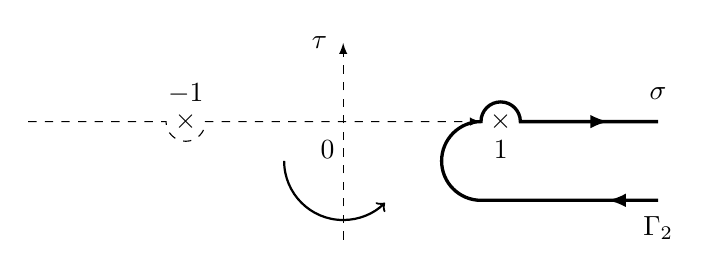
\begin{tikzpicture}
%\node at (-0.5,0) {  $\times$};
\node at (-0.2,-0.35) { $0$};
\node at (2,0) { $\times$}; % Pole
\node at (2,-0.36) { $1$};

\node at (-2,0) { $\times$};
\node at (-2,0.36) {  $-1$}; %pole
\node at (4,-1.35) { $\Gamma_2$};

\draw[dashed, decoration={markings,
 mark=at position 1.0 with {\arrow{latex}}},
      postaction={decorate}] (-4,0) -- (-2.25,0) arc (-180:0:0.25)-- (1.75,0);
      
\node at (4,0.35) {$\sigma$};

\draw[dashed, decoration={markings,
 mark=at position 1.0 with {\arrow{latex}}},
      postaction={decorate}] (0,-1.5) -- (0,1);
\node at (-0.3,1) {$\tau$};      

%\node at (2.5,-0.4) {$(\Gamma_0)$};
      
\draw[ thick, ->] (-0.75,-0.5) arc (0:135:-0.75); 
  

\draw[very thick, black, yshift=0pt,
decoration={ markings,  
      mark=at position 0.1 with {\arrow{latex}},
      mark=at position 0.9 with {\arrow{latex}}},
      postaction={decorate}]
      (4,-1) -- (1.75,-1)  arc (90:-90:-0.5) -- (1.75,0) arc(180:0:0.25)  -- (4,0);
\end{tikzpicture}
\caption
[Contour $\Gamma_2$]
{Contour $\Gamma_2$. The curved arrow shows the deformation of $\Gamma_0$ (dashed line) into $\Gamma_2$.}
\label{chapter5:figure8}
\end{figure}

During this contour deformation, only the poles
\begin{equation}
\lambda = \xi, \quad \text{with } {\rm Im}(\xi) <0 
\end{equation}
of the $DM$ function \eqref{DM_operator} are crossed and therefore, applying the residue theorem, we have for $\xi \in \mathbb{C}$, ${\rm Im}(\xi) <0$, $j=1,2$, 
\begin{equation}
\label{DM_propag_sol}
DM(X_j)(\xi) = \int_{\Gamma_0} DM(\xi,\lambda) X_j(\lambda) \, {\rm d} \lambda  = \int_{\Gamma_2} DM(\xi,\lambda) X_j(\lambda) \, {\rm d} \lambda + m(\xi) X_j(\xi).
\end{equation}

The poles of the $TM$ function \eqref{TM_operator} are
$$ \lambda = T_0^{-1}(\xi) = \xi \, \cos \widetilde{2\varphi}  - \sin \widetilde{2\varphi} \, \zeta_0(\xi) = \cos (\theta - \widetilde{2\varphi}) \quad \text{if} \quad \xi = \cos \theta $$
$T_0^{-1}$ operates in the domain $\Omega_0^-$, therefore they are crossed during this contour deformation if and only if $\xi \in \Omega_0^-$ (see dotted area on Fig.~\ref{chapter5:figure11}).
The domain $\Omega_0^-$ is delineated by the hyperbola 
\begin{equation}
\partial \Omega_0^- = \{   \xi \in \mathbb{C}, \ {\rm Im}(\xi) <0,  \xi = \cos \theta, {\rm Re} \, \theta = \widetilde{2\varphi} \}.
\end{equation}
Domain $\Omega_0^-$ and contour $\partial \Omega_0^-$ are illustrated on Fig.~\ref{chapter5:figure11}.   

Applying the residue theorem to the $TM$ integral operator then gives for $\xi \in \mathbb{C}$, ${\rm Im}(\xi) <0$, $j=1,2$,
\begin{equation}
\label{TM_propag_sol}
TM(X_j)(\xi) = \int_{\Gamma_0} TM(\xi,\lambda) X_j(\lambda) \, {\rm d} \lambda  = \int_{\Gamma_2} TM(\xi,\lambda) X_j(\lambda) \, {\rm d} \lambda + m(\xi) \, X_j[T_0^{-1}(\xi)] \mathbf{1}(\xi \in \Omega_0^-)
\end{equation}

\begin{figure}[ht]%
\begin{center}
	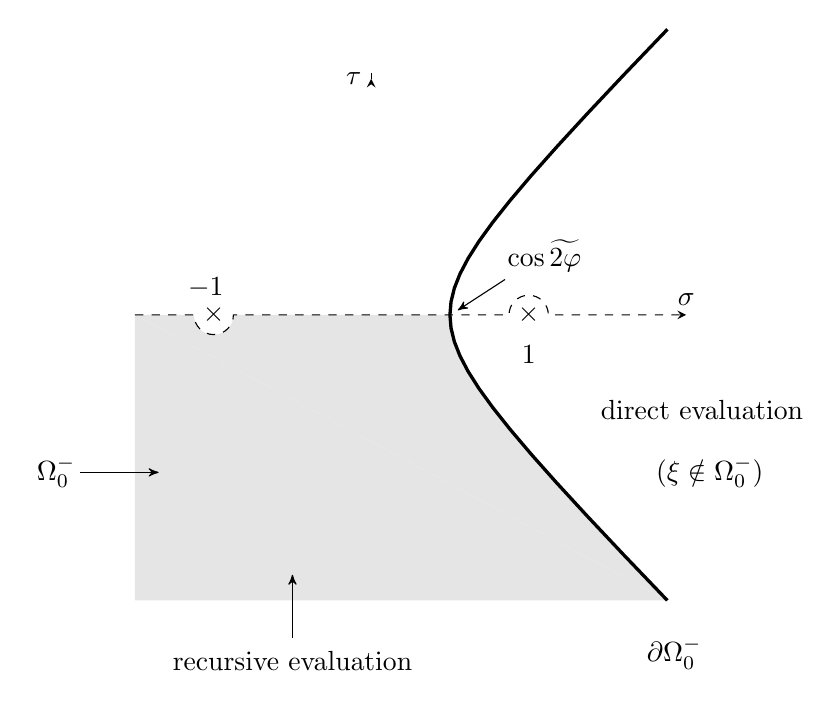
\begin{tikzpicture}
		% Filling Omega_0^-
	\fill [color=gray!20]
	(-1,0)
	-- plot [domain= 0:2] ({cosh(\x)},{-sinh(\x)})
	-- (-3,0)
	-- cycle;
	
	\fill [color=gray!20]
	({cosh(2)},{-sinh(2)})
	-- plot [domain= 0:-3] ({\x},{-sinh(2)})
	-- (-3,0)
	-- cycle;
	
	\fill[color=white] (-2,0) circle (0.25);
	
	\draw[dashed, ->,>=stealth] (-3,0)  -- (-2.25,0) arc(-180:0:0.25)--(1.75,0) arc (180:0:0.25)--(4,0) node[above]{$\sigma$};
	\draw[dashed, ->,>=stealth](0,3)--(0,3) node[left]{$\tau$};
	
	\node at (2,0) {$\times$}; % Pole
	\node at (2,-0.5) {$1$};
	\node at (-2,0) { $\times$};
	\node at (-2.1,0.35) {$-1$}; %pole
	
	% Hyperbola (contour  partial_Omega_0 )
	\draw[black, very thick][domain=-2:2] plot({cosh(\x)}, {-sinh(\x)});
	\node at (3.85,-4.3) {$\partial \Omega_0^-$};
	\draw[thin, ->,>=stealth'](1.7,0.45) -- (1.1, 0.06);
	\node at (2.2, 0.75) {$\cos \widetilde{2\varphi}$};
	
	% Omega_0
	\node at (-4,-2) {$\Omega_0^-$};
	\draw[->,>=stealth'] (-3.7, -2) -- (-2.7,-2);
	\draw[->,>=stealth'] (-1,-4.1) -- (-1,-3.3);
	\node at (-1,-4.4) {recursive evaluation};
	\node at (4.2,-1.2) { direct evaluation};
    \node at (4.3,-2) { $(\xi \notin \Omega_0^-)$};
	
	\end{tikzpicture}
\end{center}
\caption
[Domain $\Omega_0^-$ and its lower boundary $\partial \Omega_0^-$]
{Domain $\Omega_0^-$ and its lower boundary $\partial \Omega_0^-$ in the complex plane $\xi=\sigma + i \tau$. $\Omega_0^-$ is delimited by $\partial \Omega_0^-$ andthe semi-axis $]-\infty, \cos \widetilde{2\varphi}]$. }
\label{chapter5:figure11}
\end{figure}


Using \eqref{DM_propag_sol} and \eqref{TM_propag_sol} in the system of functional equations \eqref{sys_regular}, the system \eqref{sys_regular} is then equivalent to this new system for $\xi \in \mathbb{C}$, ${\rm Im}(\xi) <0$:
\begin{equation}
\label{propag_sol_sys}
\begin{cases}
X_1(\xi) = g_1(\xi) -  X_2(T_0^{-1}(\xi)) \, \mathbf{1}(\xi \in \Omega_0^-) \\
\\
X_2(\xi) = g_2(\xi) - X_1(T_0^{-1}(\xi)) \, \mathbf{1}(\xi \in \Omega_0^-) 
\end{cases}
\end{equation}
where
\begin{equation}
g_j(\xi) = m(\xi)^{-1} \left[ u_j(\xi) - \int_{\Gamma_2} DM(\xi,\lambda) \, X_j(\lambda) \, {\rm d} \lambda - \int_{\Gamma_2} TM(\xi,\lambda) \, X_{3-j}(\lambda) \, {\rm d} \lambda \right] \\
\end{equation}
Formula \eqref{propag_sol_sys} is called the recursive formula because it uses the value of the regular function $X_2$ at point $T_0^{-1}(\xi)$ to compute the value of $X_1$ at the point $\xi$ where the approximation is not valid (and vice-versa). If the translation from $\xi$ to $T_0^{-1}(\xi)$ is not sufficient to reach the domain $\mathbb{C} \backslash \Omega_0^-$ where the approximation is valid, then the use of the formula is repeated as many times as necessary (computing $X_2(T_0^{-1}(\xi))$ using the value of $X_1(T_0^{-2}(\xi))$, etc.).

To calculate $g_j$ functions, we need to compute
\begin{equation*}
\int_{\Gamma_2} DM(\xi,\lambda) \, X_j(\lambda) {\rm d} \lambda =\sum_k \tilde{X}_j^k \int_{\Gamma_2} DM(\xi,\lambda) \, \varphi_k(\lambda) \, {\rm d} \lambda 
\end{equation*}
and
\begin{equation*}
\int_{\Gamma_2} TM(\xi,\lambda) \, X_j(\lambda) {\rm d} \lambda = \sum_k \tilde{X}_j^k \int_{\Gamma_2} TM(\xi,\lambda) \, \varphi_k(\lambda) \, {\rm d} \lambda
\end{equation*}

If ${\rm Im}(a) < 0$, the residue theorem combined with the variable change $\lambda = iy$  yields
\begin{equation}
\int_{\Gamma_2} DM(\xi,\lambda) \,  \dfrac{1}{\lambda+a} \, \, {\rm d} \lambda =  \dfrac{1}{2\pi} \, \mathcal{D}(a,\xi) - \dfrac{m(\xi)}{\xi +a} = \mathcal{ND}(a,\xi). 
\end{equation}

For the $TM$ contributions, the poles $\lambda = T_0^{-1}(\xi)$ are taken into account if and only if $\xi \in \Omega_0^-$. Thus, for $\xi \in \Omega_0^-$, ${\rm Im}(a) < 0$, the residue theorem combined with the variable change $\lambda = iy$ gives
\begin{equation}
\int_{\Gamma_2} TM(\xi,\lambda) \,  \dfrac{1}{\lambda +a} \, \, {\rm d} \lambda = \frac{1}{2i\pi} \mathcal{T}(a,\xi)- \dfrac{m(\xi)}{T_0^-(\xi) +a}   =  \mathcal{NT}(a,\xi)
\end{equation}

Formula \eqref{regular_part_decomp} finally leads to, for $\xi \in \Omega_0^-$ and $j=1,2$,
\begin{eqnarray}
m(\xi)\, g_j(\xi) -  u_j(\xi)=
-\Big( \sum_k \tilde X_j^{k}\, d_k \, N\mathcal D(a_k,\xi)+\sum_k \tilde X_{3-j}^{k} \, d_k \,
N\mathcal T(a_k,\xi) \Big) \nonumber
\end{eqnarray}

Some numerical results are presented in the sequel.

\section{Numerical results}
\label{Chapter5:results}

In this section, a far-field ($k_0r>>1$) asymptotic evaluation of the diffraction coefficient is computed using the stationary phase method :
\begin{equation}
\label{GTDCoeff_SF}
D(\theta) = \dfrac{e^{-i\frac{\pi}{4}}}{\sqrt{2\pi}} \, [\hat{\alpha}_1( - \cos \theta) + \hat{\alpha}_2( - \cos ( 2\varphi - \theta))]
\end{equation}
where $\hat{\alpha}_1$ and $\hat{\alpha}_2$ are the spectral functions, is compared to the analytic expression of the diffraction coefficient of the scattering of a plane wave with a wedge at interfaces fluid/void as expressed by Sommerfeld \cite{Sommerfeld}. Keller \cite{GTD} gives an analytical expression of the GTD approximation of the coefficient in the case of the diffraction of a scalar plane wave by a wedge with Dirichlet boundaries which can be used in the case of a stress-free wedge immersed in a fluid :
\begin{align}
\label{GTDCoeff_Dir}
D^{\rm (Dir)}(\theta) = \dfrac{e^{i\frac{\pi}{4}}}{2N \sqrt{2\pi}}  \, \left[ \cot \left( \dfrac{\pi + (\theta + \theta_{\rm inc})}{2N} \right) + \cot \left( \dfrac{\pi - (\theta + \theta_{\rm inc})}{2N} \right) \right.   \nonumber \\
\left. - \cot \left( \dfrac{\pi + (\theta - \theta_{\rm inc})}{2N} \right) - \cot \left( \dfrac{\pi - (\theta - \theta_{\rm inc})}{2N} \right) \right],
\end{align}
with $N=2\varphi/\pi$.

To apply the recursive procedure described in \ref{propag_sol}, calculation points $\xi$ must have a negative imaginary part. The calculation points considered are then
\begin{equation}
\label{calculation_points_recursive}
\xi_1 = -\cos \theta -i\,10^{-3}  \quad \text{and} \quad \xi_2=- \cos (2\varphi - \theta) - i\, 10^{-3} ,
\end{equation}
where $\theta$ is the observation angle in the wedge (see Fig.~\ref{chapter5:figure1}).

For the Galerkin basis defined in \eqref{Galerkin_basis}, the parameters $a_k \in [1,\infty[$ are chosen as an exponential law \cite{CroisilleLebeau}:
\begin{equation}
\begin{split}
\label{bas_Gal}
a_k &= 1.1 + 0.05 \left( 10^{\frac{k -1}{4}} - 1 \right), \quad 1\leq k\leq 20 \\
b_k &= a_k  - i 0.1, \quad 1\leq k\leq 20 .
\end{split}
\end{equation}

The module of the diffraction coefficients computed using spectral functions and Sommerfeld integral method for various wedge angles are plotted in terms of the observation angle $\theta, \quad 0\leq \theta\leq 2\varphi$ and presented on Fig.~\ref{chapter5:figure12}. 
\begin{figure}[h!]
\centering
\begin{subfigure}[b]{0.49\textwidth}
        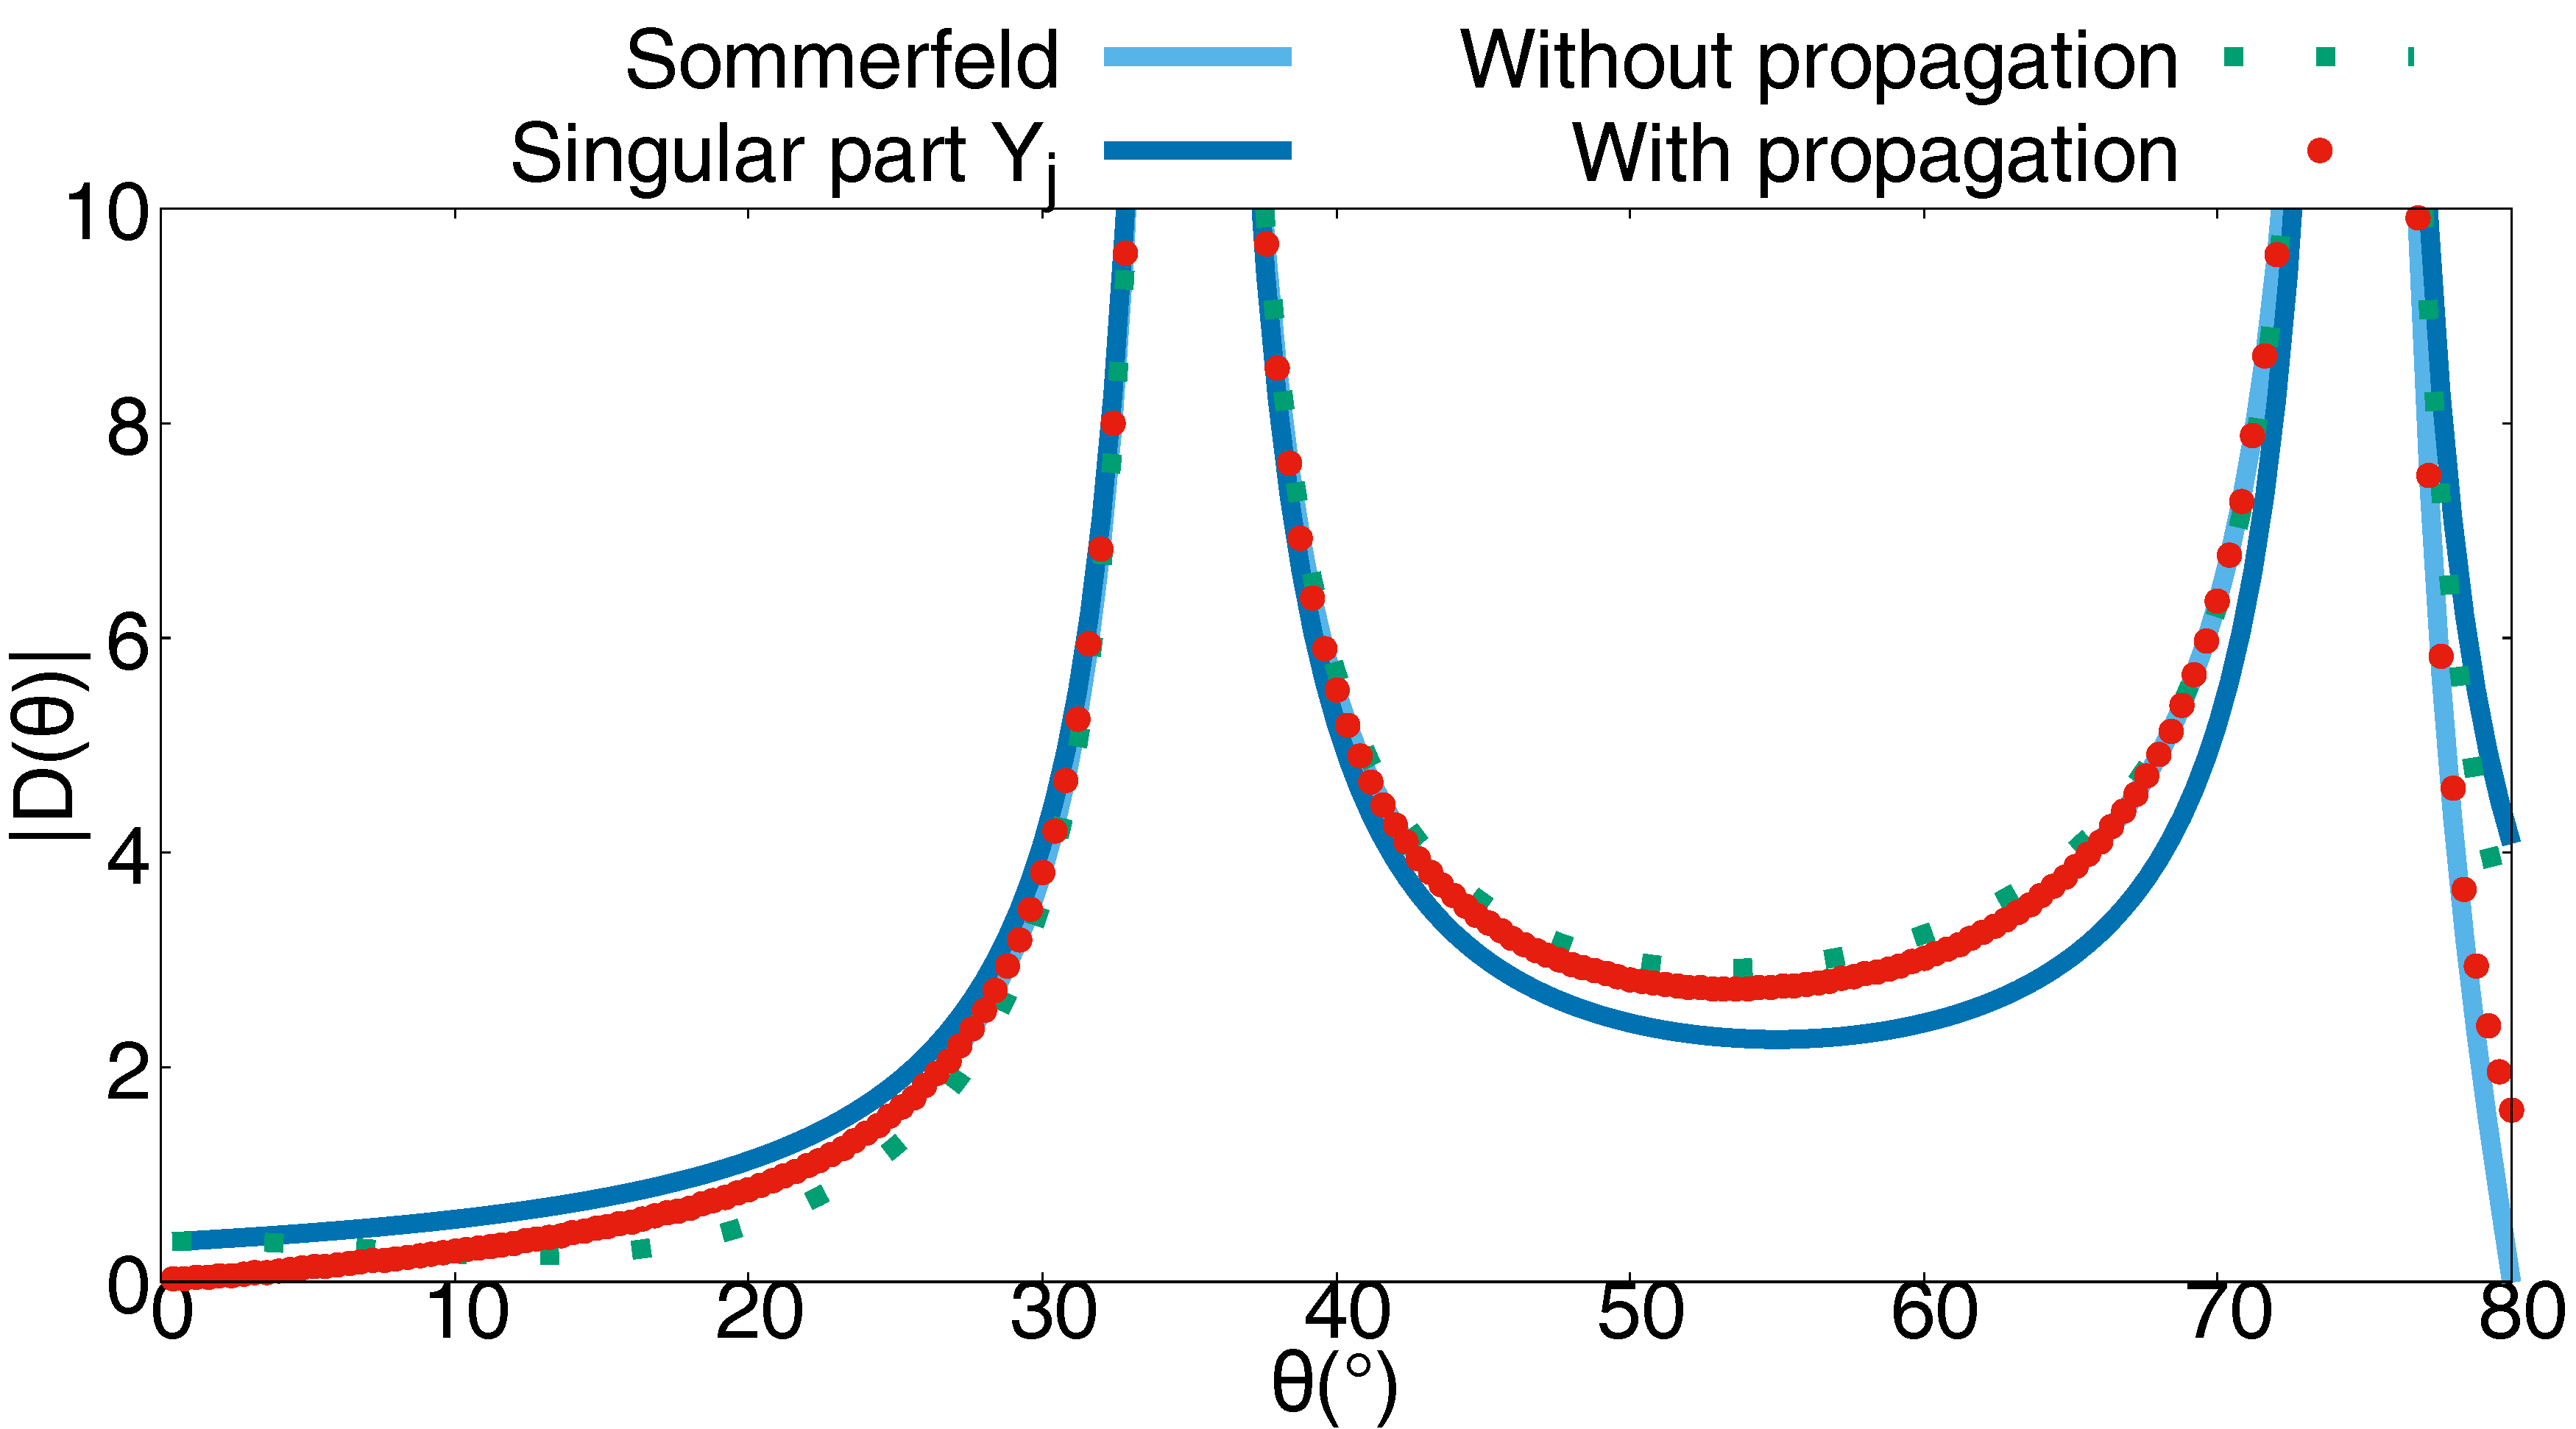
\includegraphics[width=\textwidth]{images/chapter2/Figure8a.pdf}
        \caption{$2\varphi = 80^o$, $\theta_{\rm inc} = 55^o$}
        \label{chapter5:figure12a}
    \end{subfigure}
\begin{subfigure}[b]{0.49\textwidth}
        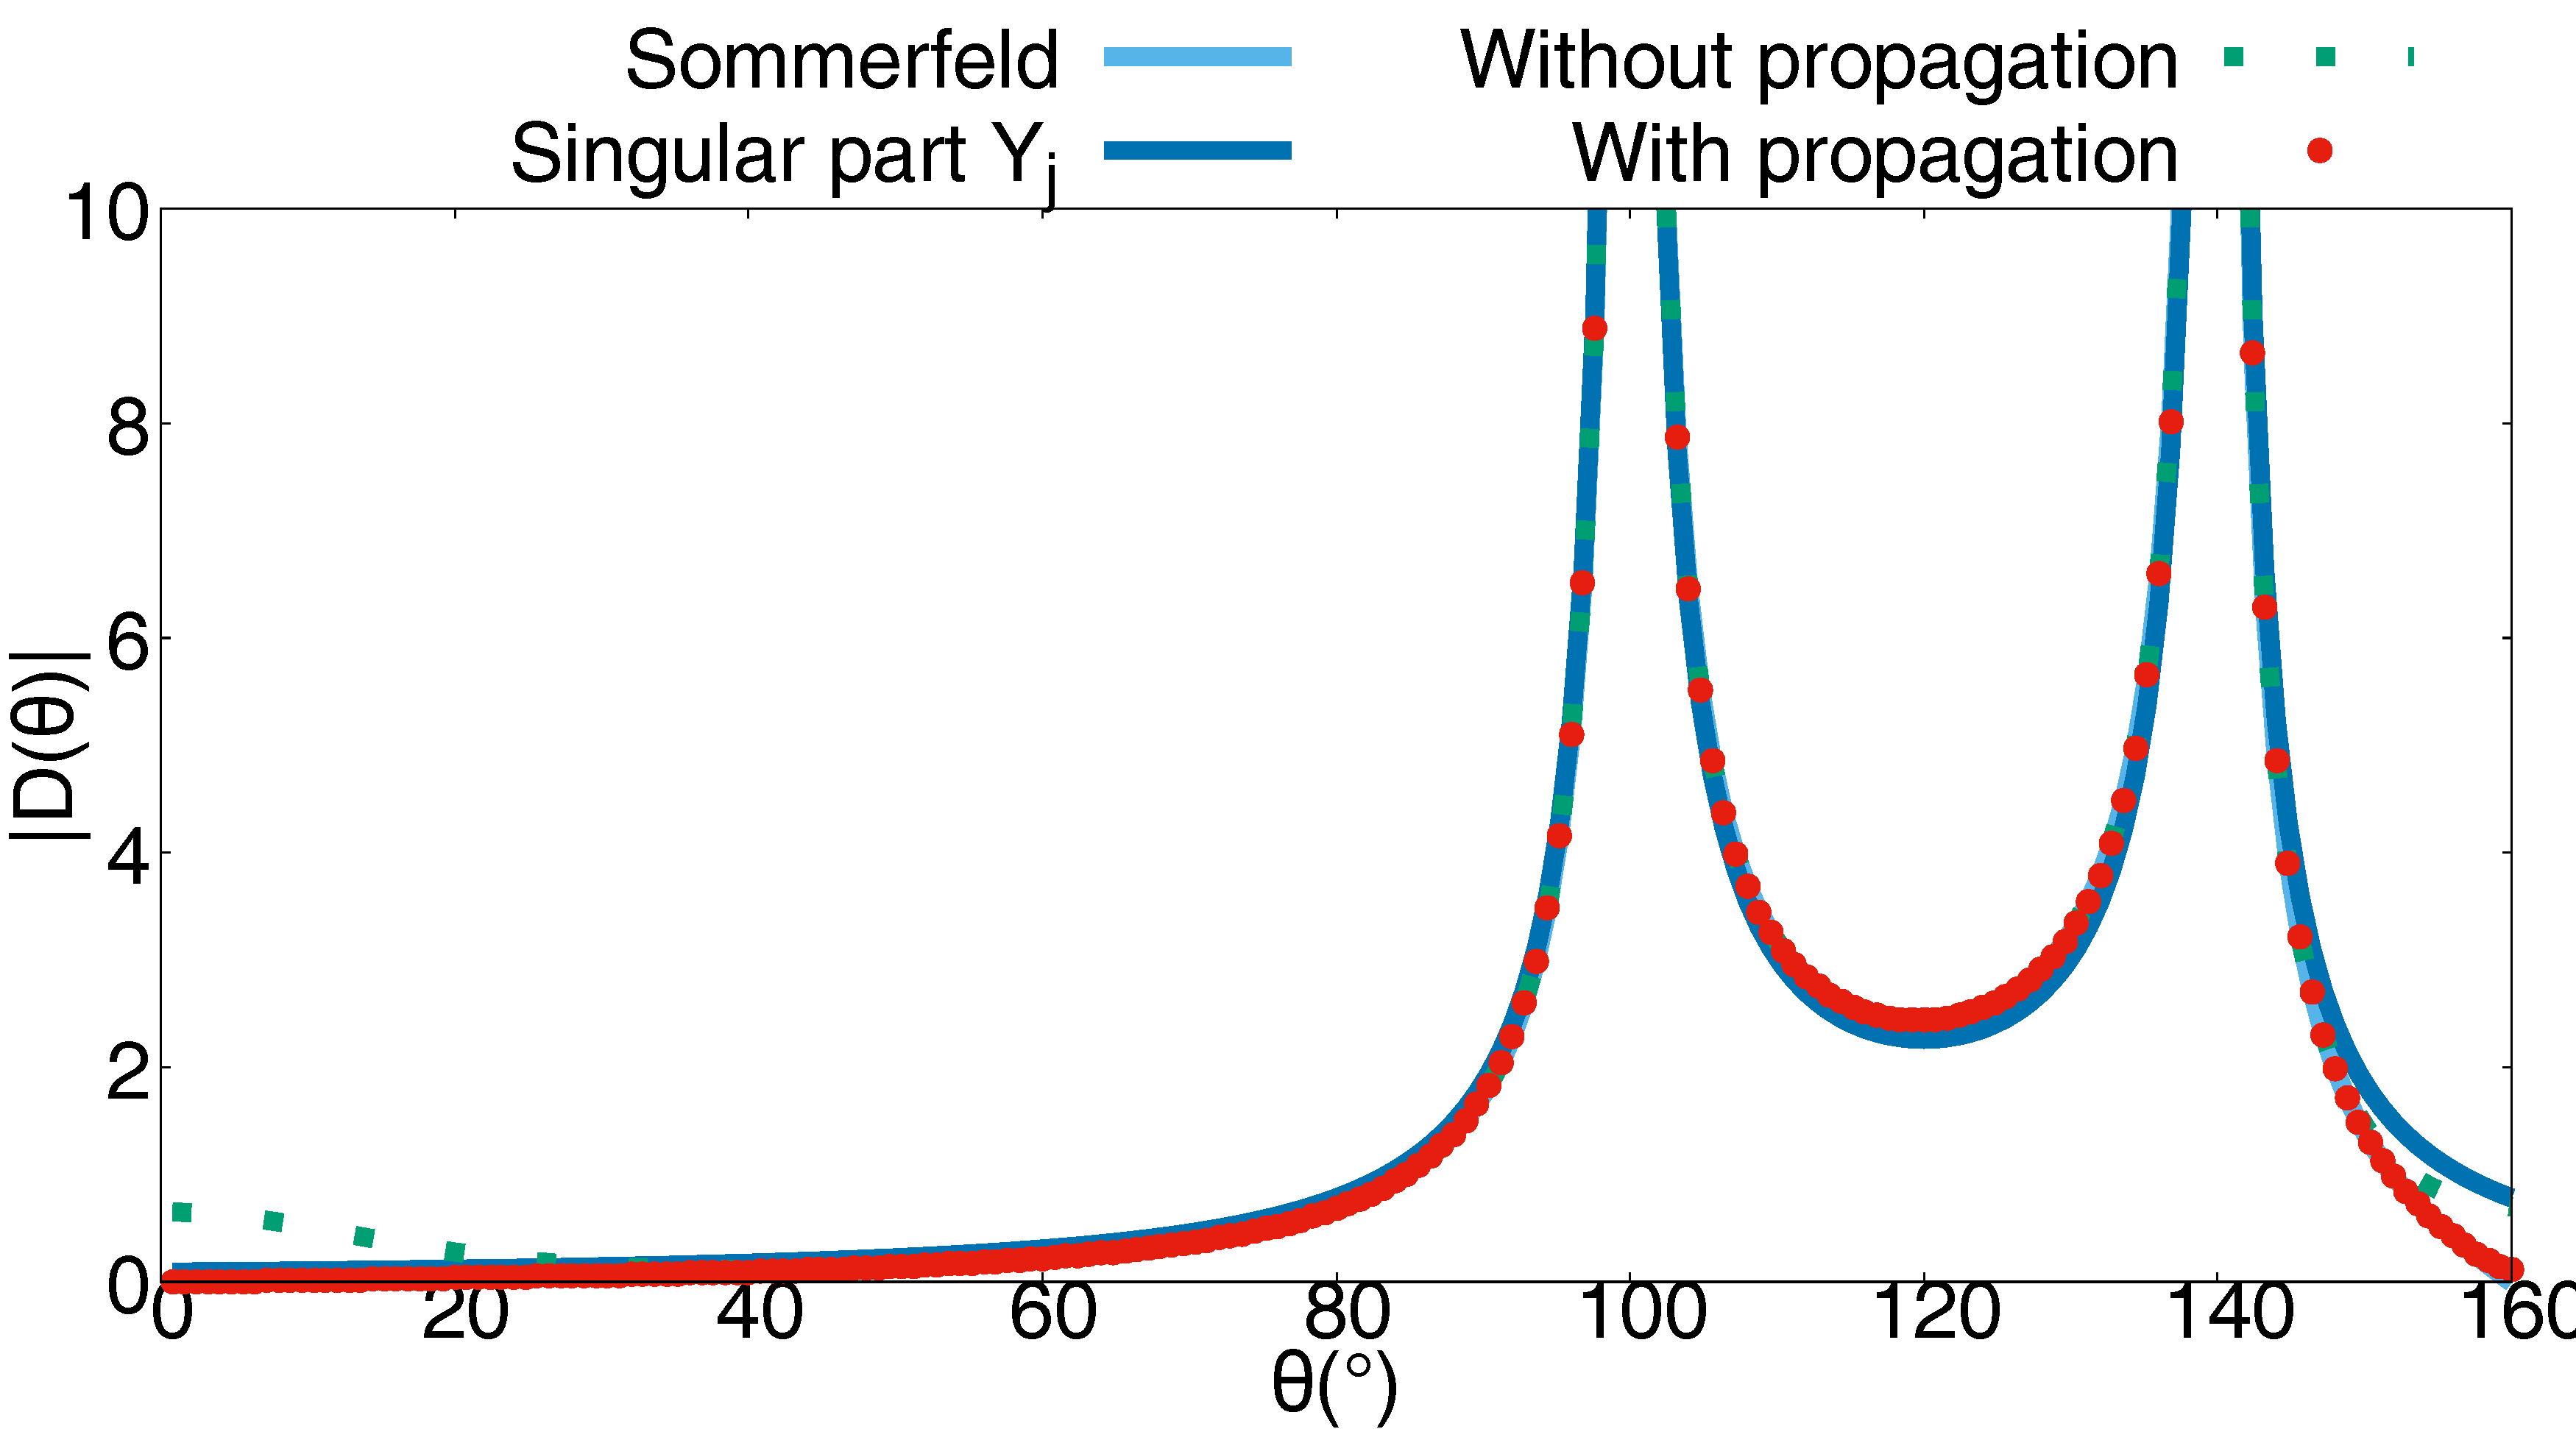
\includegraphics[width=\textwidth]{images/chapter2/Figure8b.pdf}
        \caption{$2\varphi = 160^o$, $\theta_{\rm inc} = 40^o$}
        \label{chapter5:figure12b}
    \end{subfigure}
\\
~\\
\begin{subfigure}[b]{0.49\textwidth}
        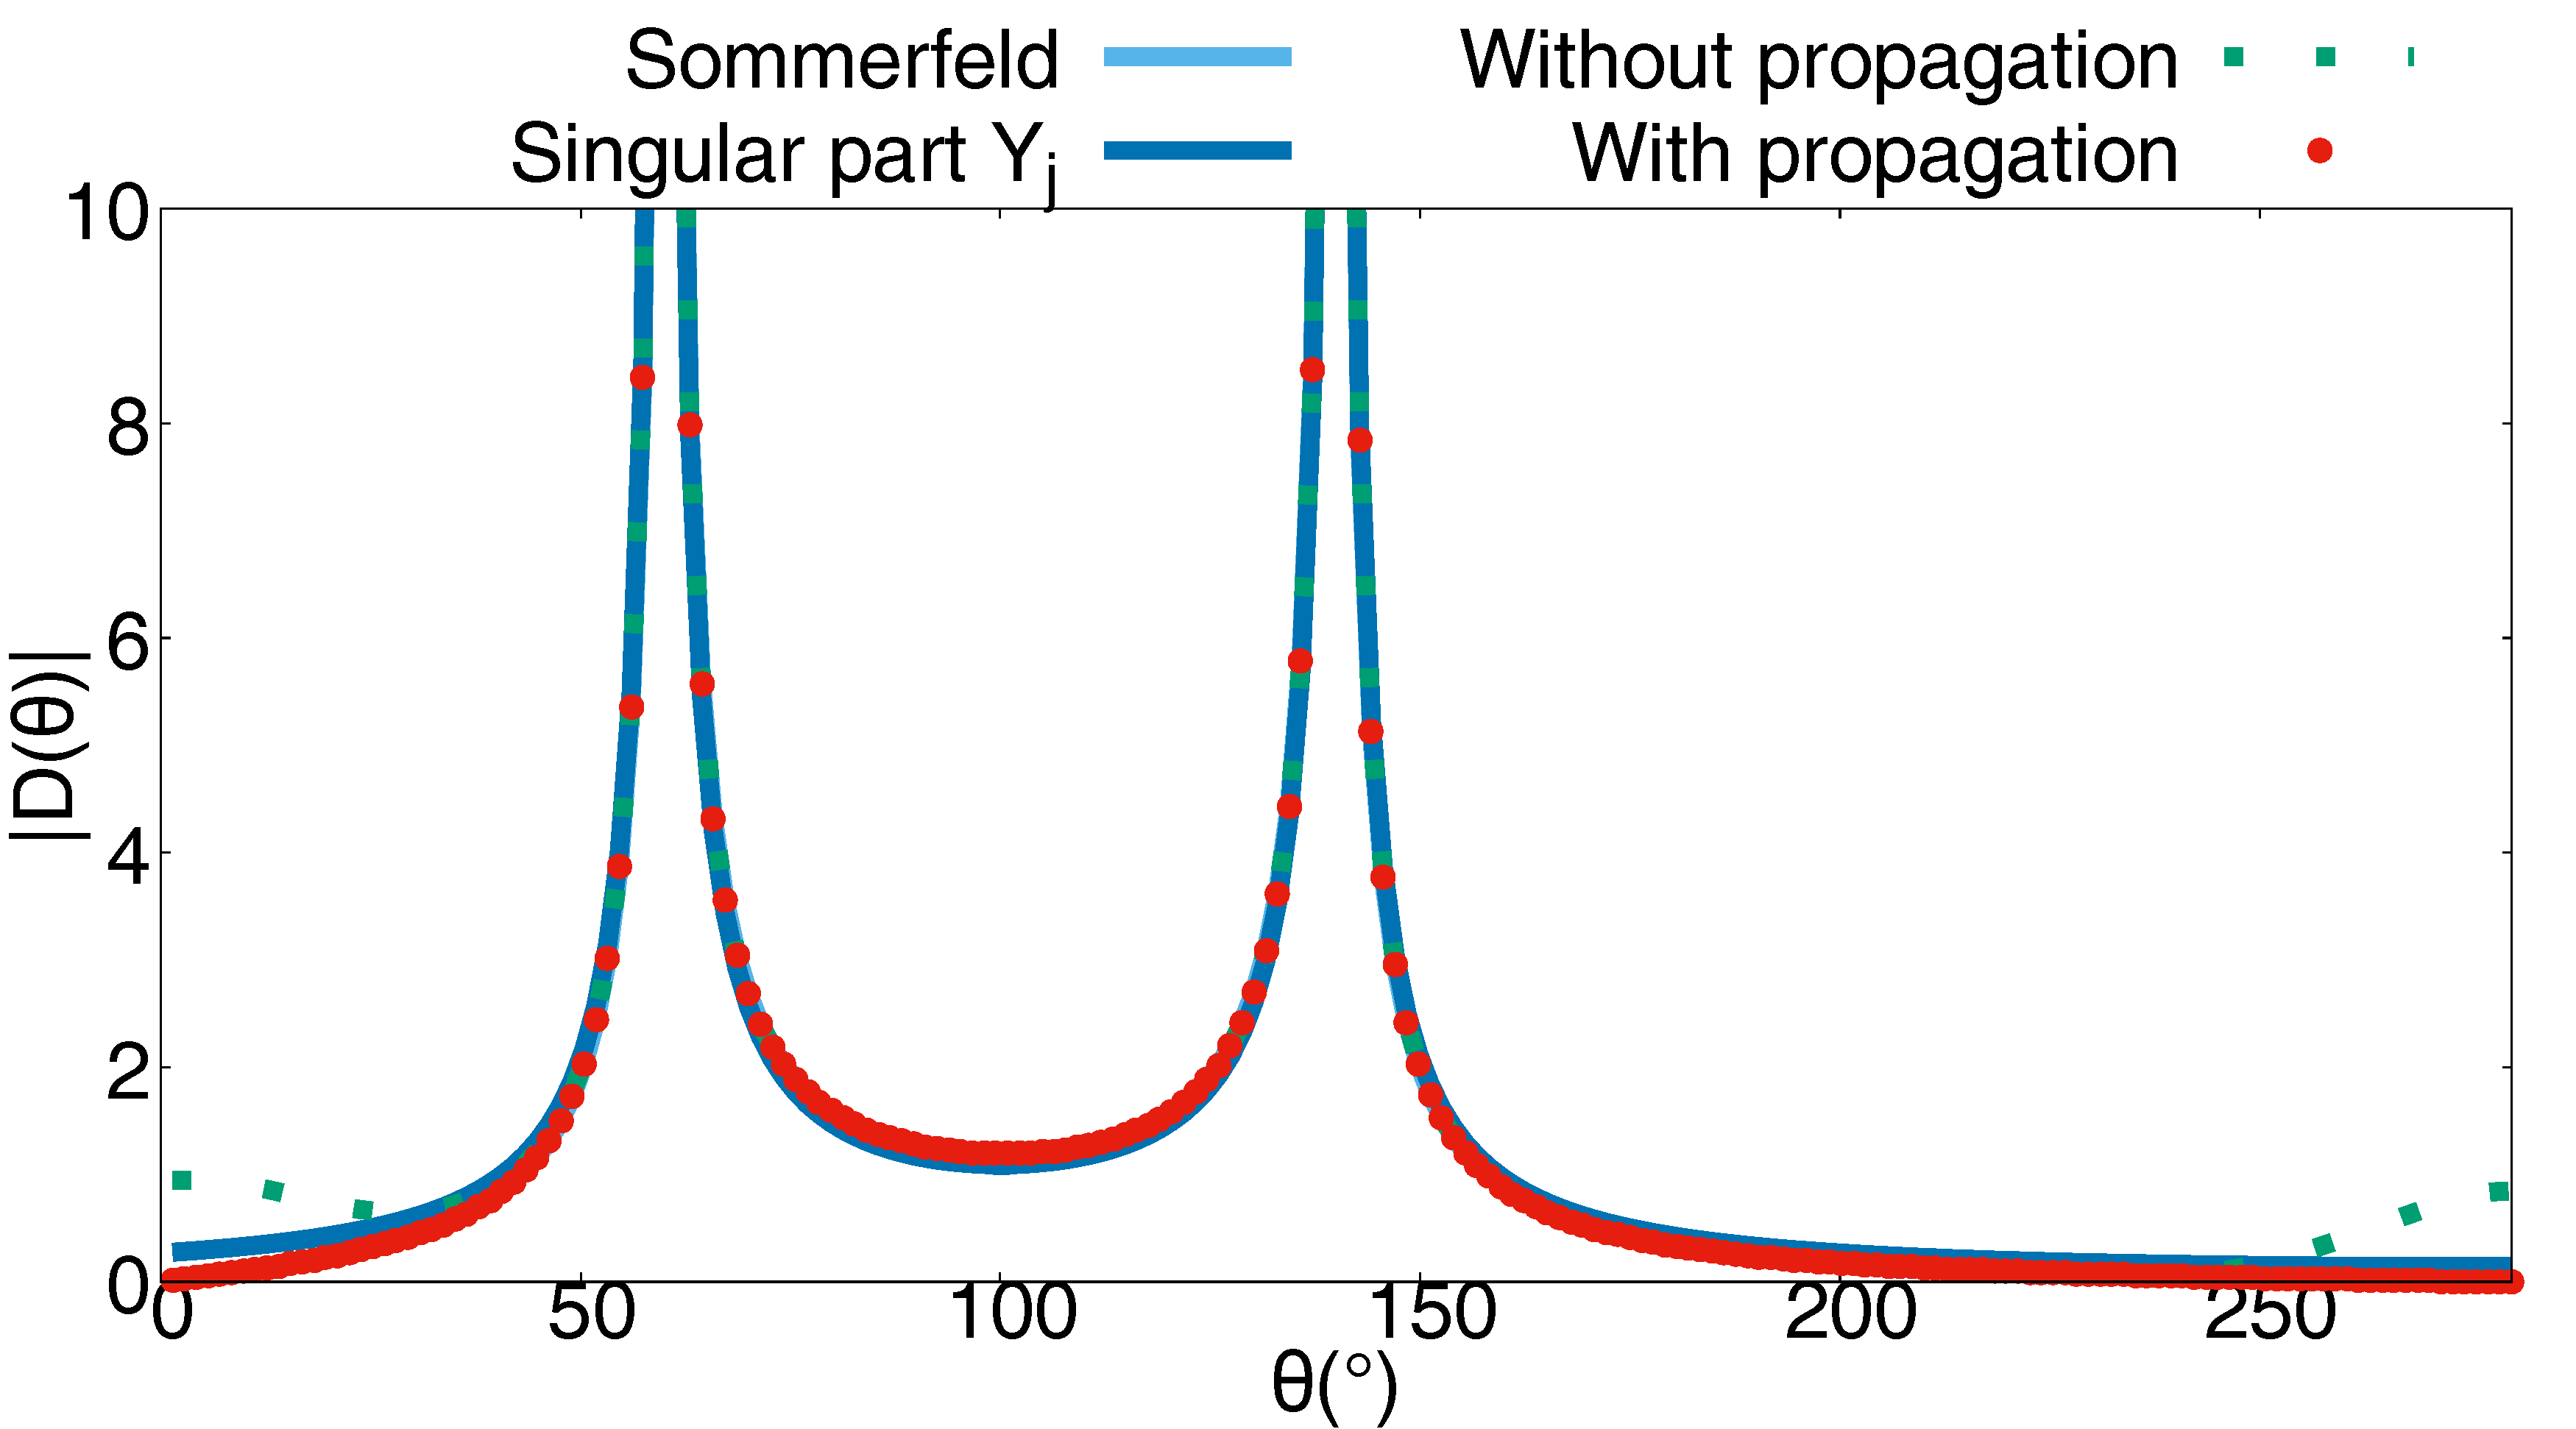
\includegraphics[width=\textwidth]{images/chapter2/Figure8c.pdf}
        \caption{$2\varphi = 280^o$, $\theta_{\rm inc} = 240^o$}
        \label{chapter5:figure12d}
    \end{subfigure}
\begin{subfigure}[b]{0.49\textwidth}
        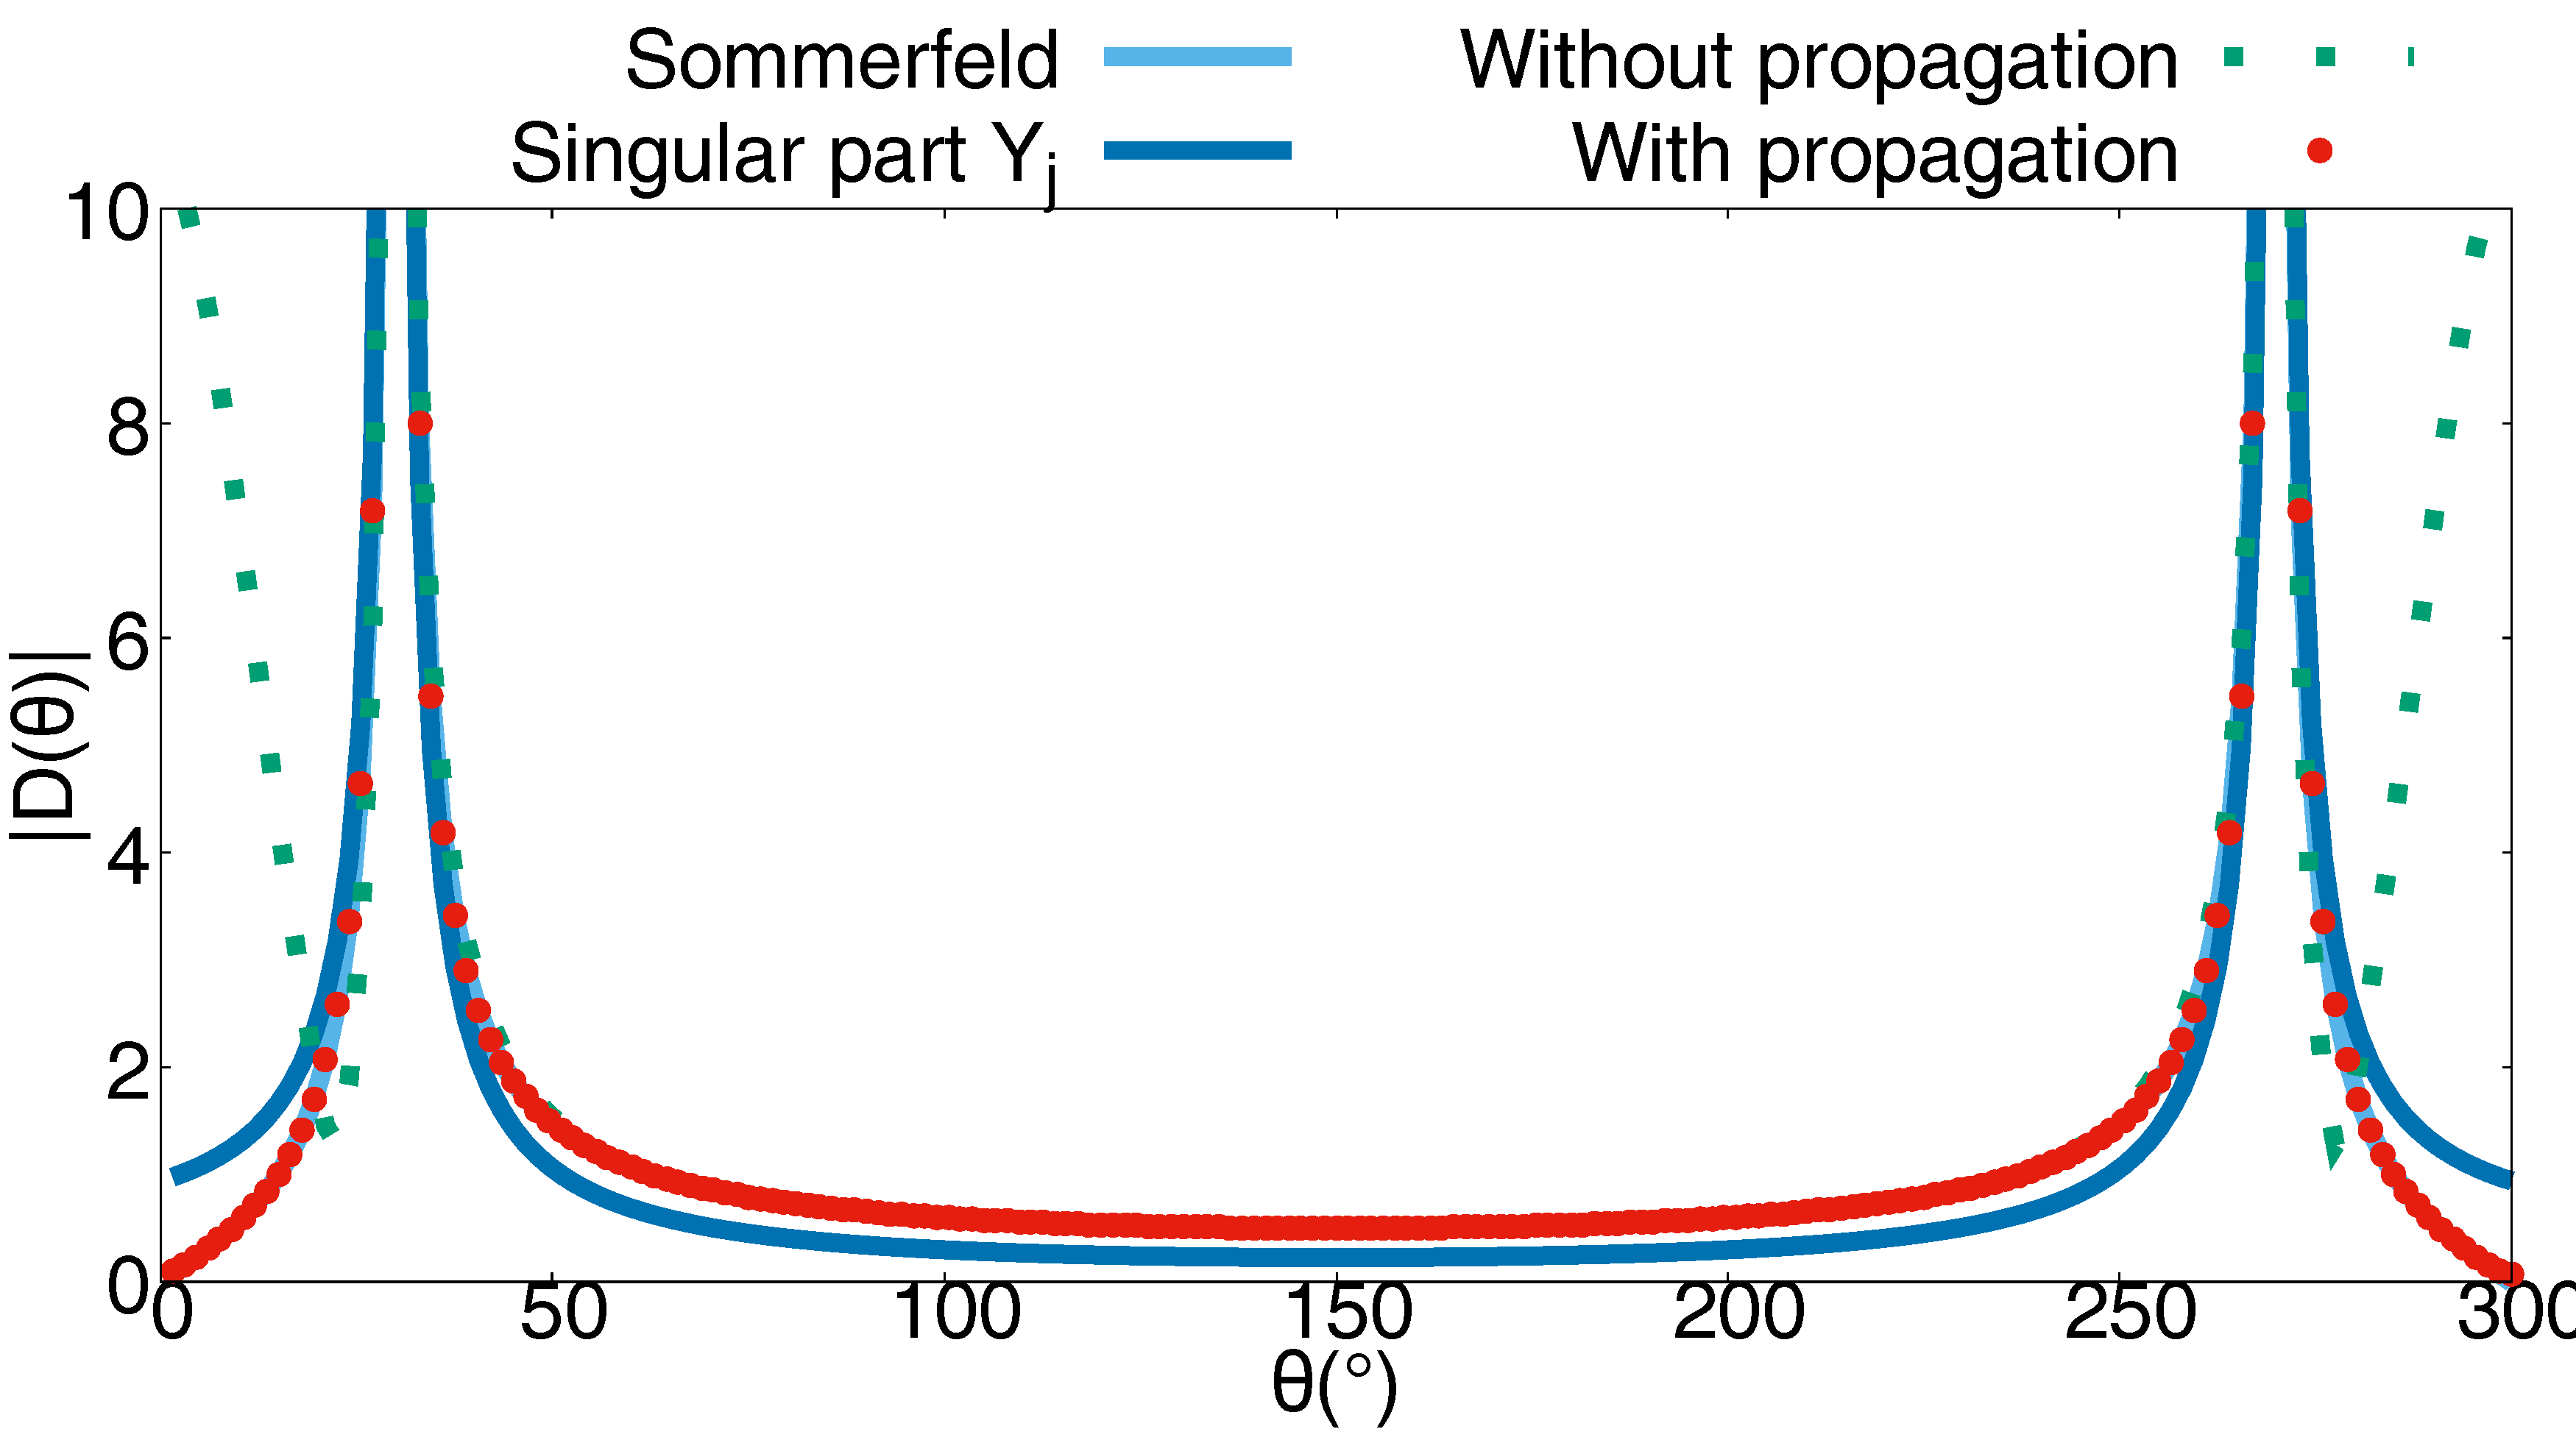
\includegraphics[width=\textwidth]{images/chapter2/Figure8d.pdf}
        \caption{$2\varphi = 300^o$, $\theta_{\rm inc} = 150^o$}
        \label{chapter5:figure12c}
    \end{subfigure}
\caption
[Diffraction coefficient computed with the recursive formula of spectral functions and with the Sommerfeld method, in the case of Dirichlet boundary conditions]
{Diffraction  coefficient computed with the spectral functions and with the Sommerfeld method, in the case of Dirichlet boundary conditions.}
\label{chapter5:figure12}
\end{figure}

In the case of Neumann boundary conditions, the initial system \eqref{Chapter5:Adimen_waveMotion} is replaced by the follwing :
\begin{equation}
\begin{cases}
(\triangle+1)v =  0 \quad \text{in } \Omega_f, \\
\partial v/\partial n =  -\partial h_{\rm inc}/\partial n \quad \quad \quad \text{on } F_j, \quad j=1,2
\end{cases},
\label{neuproblem}
\end{equation}
where n is the inward-pointing normal to the wedge faces. The spectral functions method can once again be applied following the same steps as for the Dirichlet boundary conditions. The details of the computation are not repeated here. Once again, a far-field evaluation of the diffraction, given by  \eqref{GTDCoeff_SF} is compared to the analytic expression of the diffraction coefficient given by Sommerfeld \cite{Sommerfeld}. The GTD approximation of this coefficient is also given by Keller \cite{GTD} :
\begin{align}
\label{GTDCoeff_Neu}
D^{\rm (Neu)}(\theta) = \dfrac{e^{i\frac{\pi}{4}}}{2N \sqrt{2\pi}}  \, \left[ \cot \left( \dfrac{\pi + (\theta + \theta_{\rm inc})}{2N} \right) + \cot \left( \dfrac{\pi - (\theta + \theta_{\rm inc})}{2N} \right) \right.   \nonumber \\
\left. + \cot \left( \dfrac{\pi + (\theta - \theta_{\rm inc})}{2N} \right) + \cot \left( \dfrac{\pi - (\theta - \theta_{\rm inc})}{2N} \right) \right] 
\end{align}
with $N=2\varphi/\pi$. The results are presented on Fig ~\ref{chapter5:figure13}.

\begin{figure}[h!]
\centering
\begin{subfigure}[b]{0.49\textwidth}
        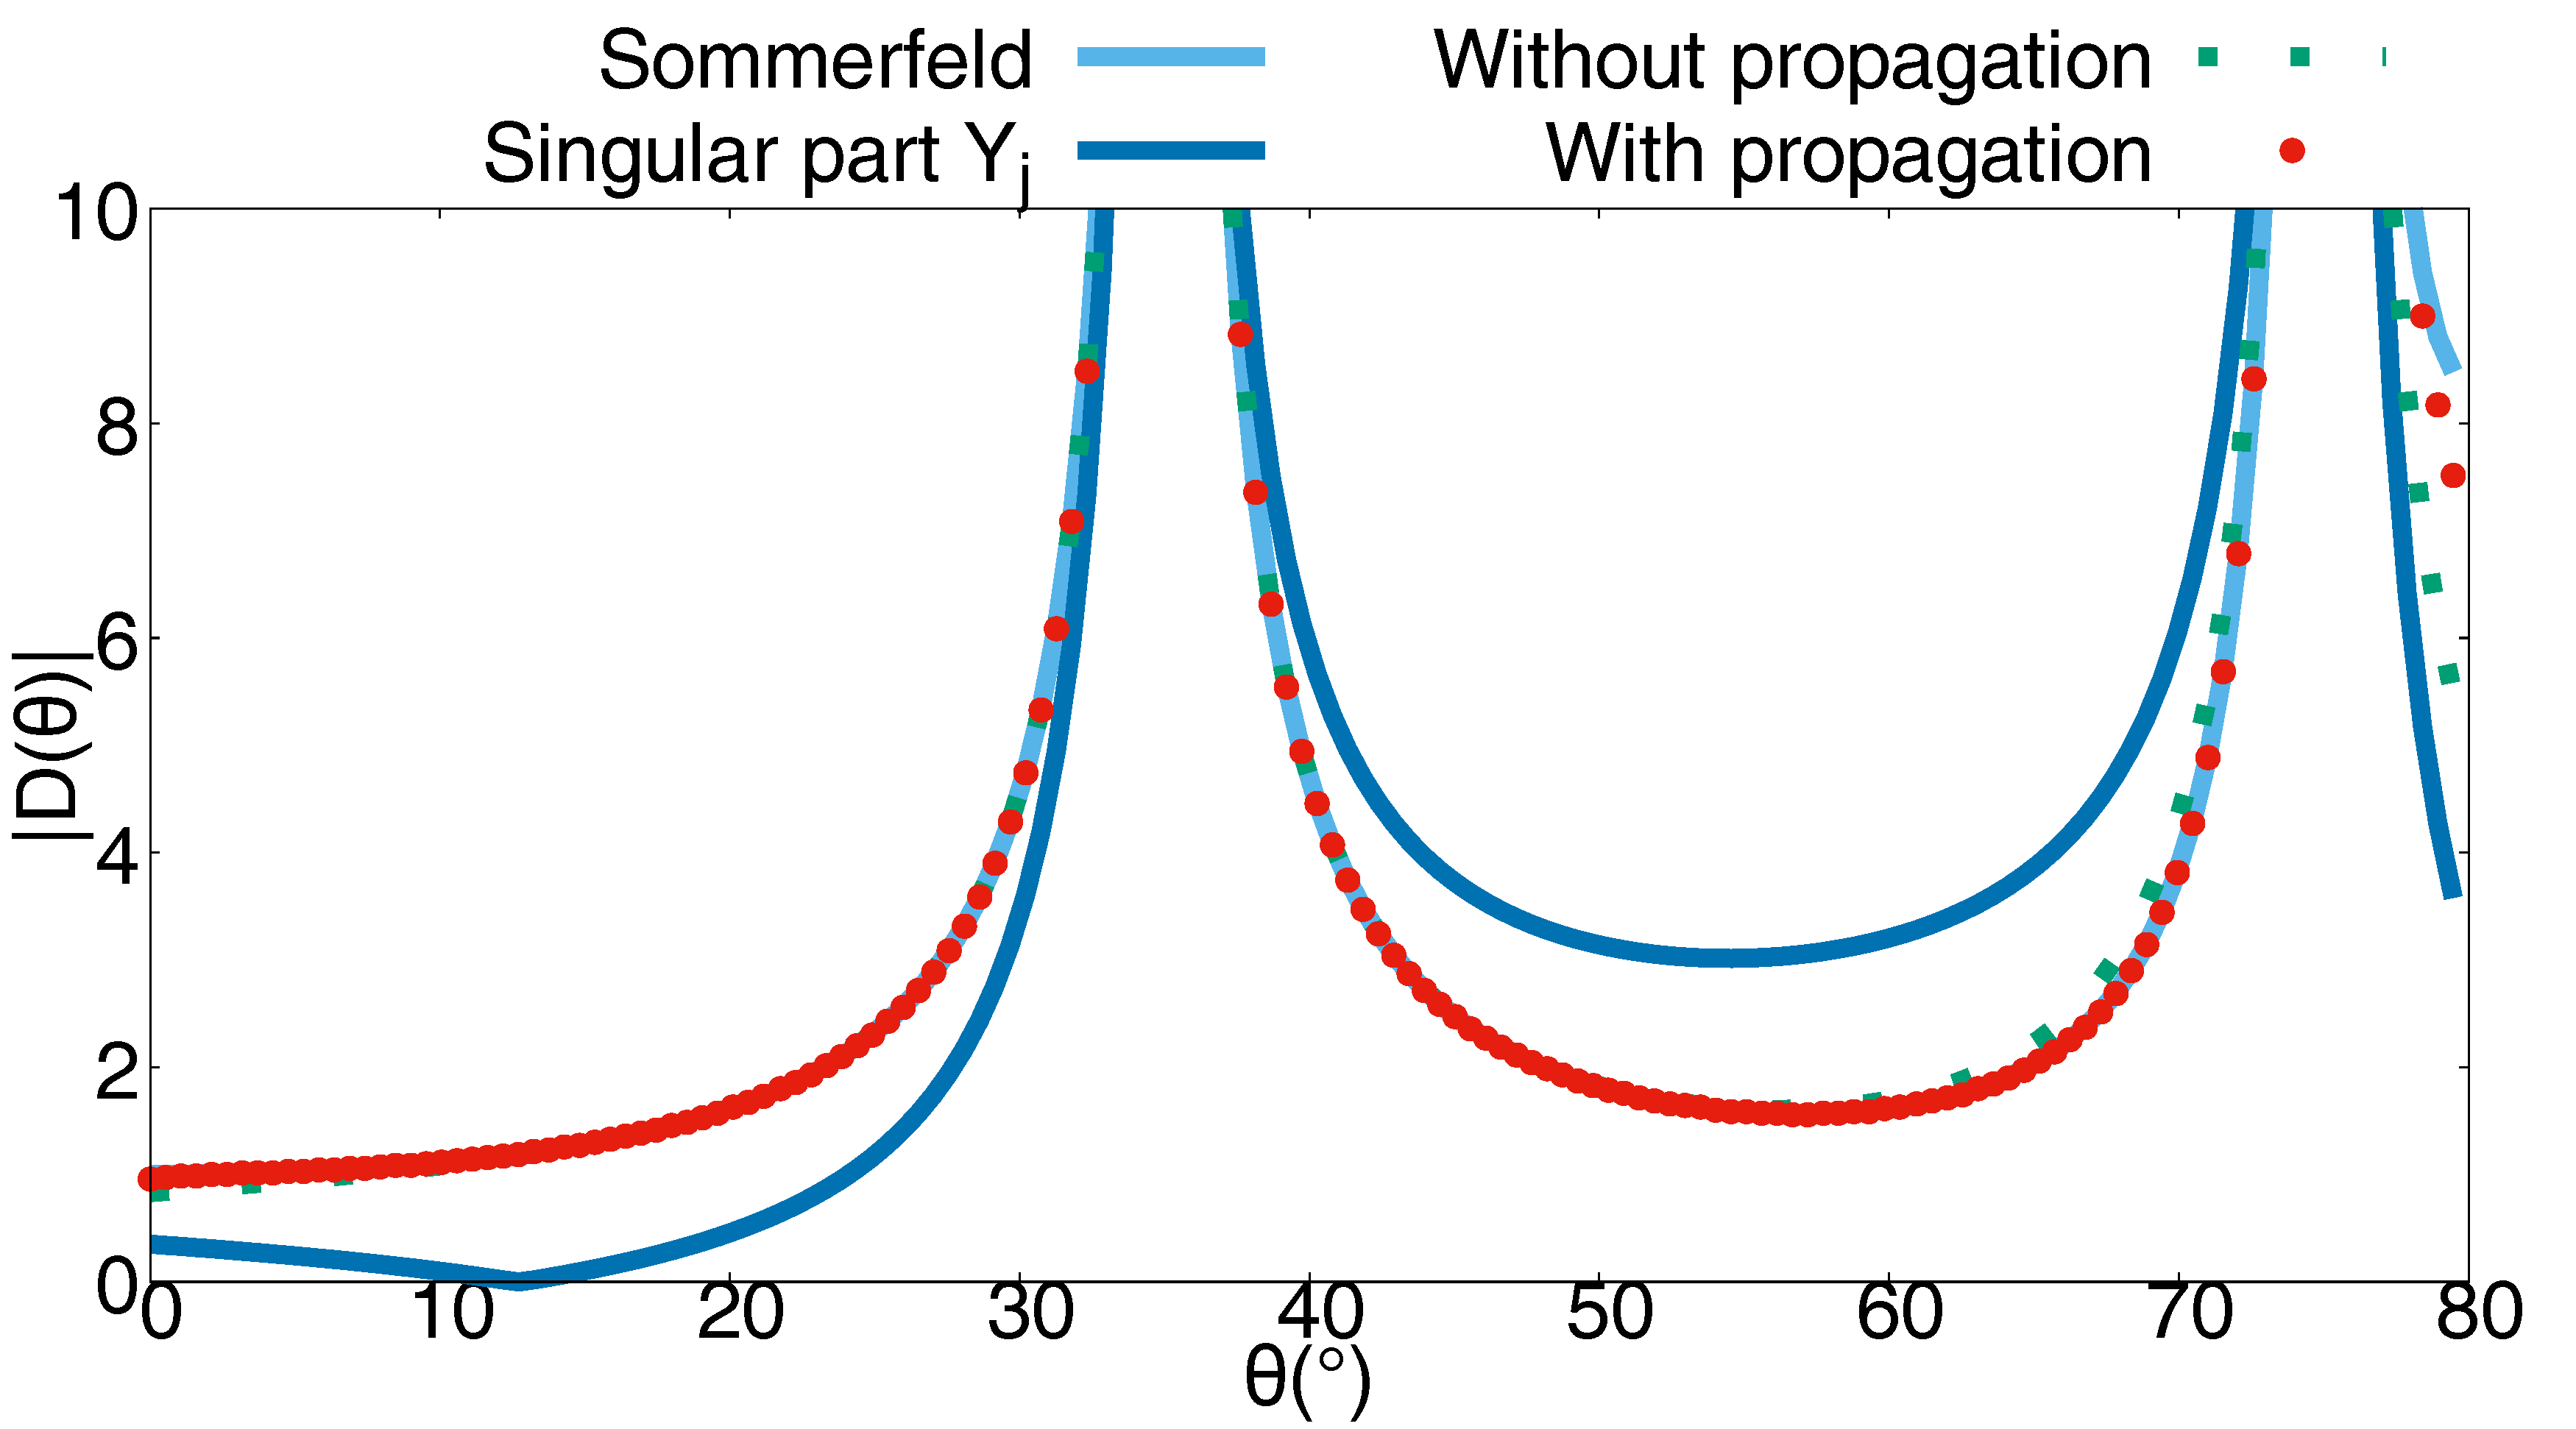
\includegraphics[width=\textwidth]{images/chapter2/Figure9a.pdf}
        \caption{$2\varphi = 80^o$, $\theta_{\rm inc} = 55^o$}
        \label{chapter5:figure13a}
    \end{subfigure}
\begin{subfigure}[b]{0.49\textwidth}
        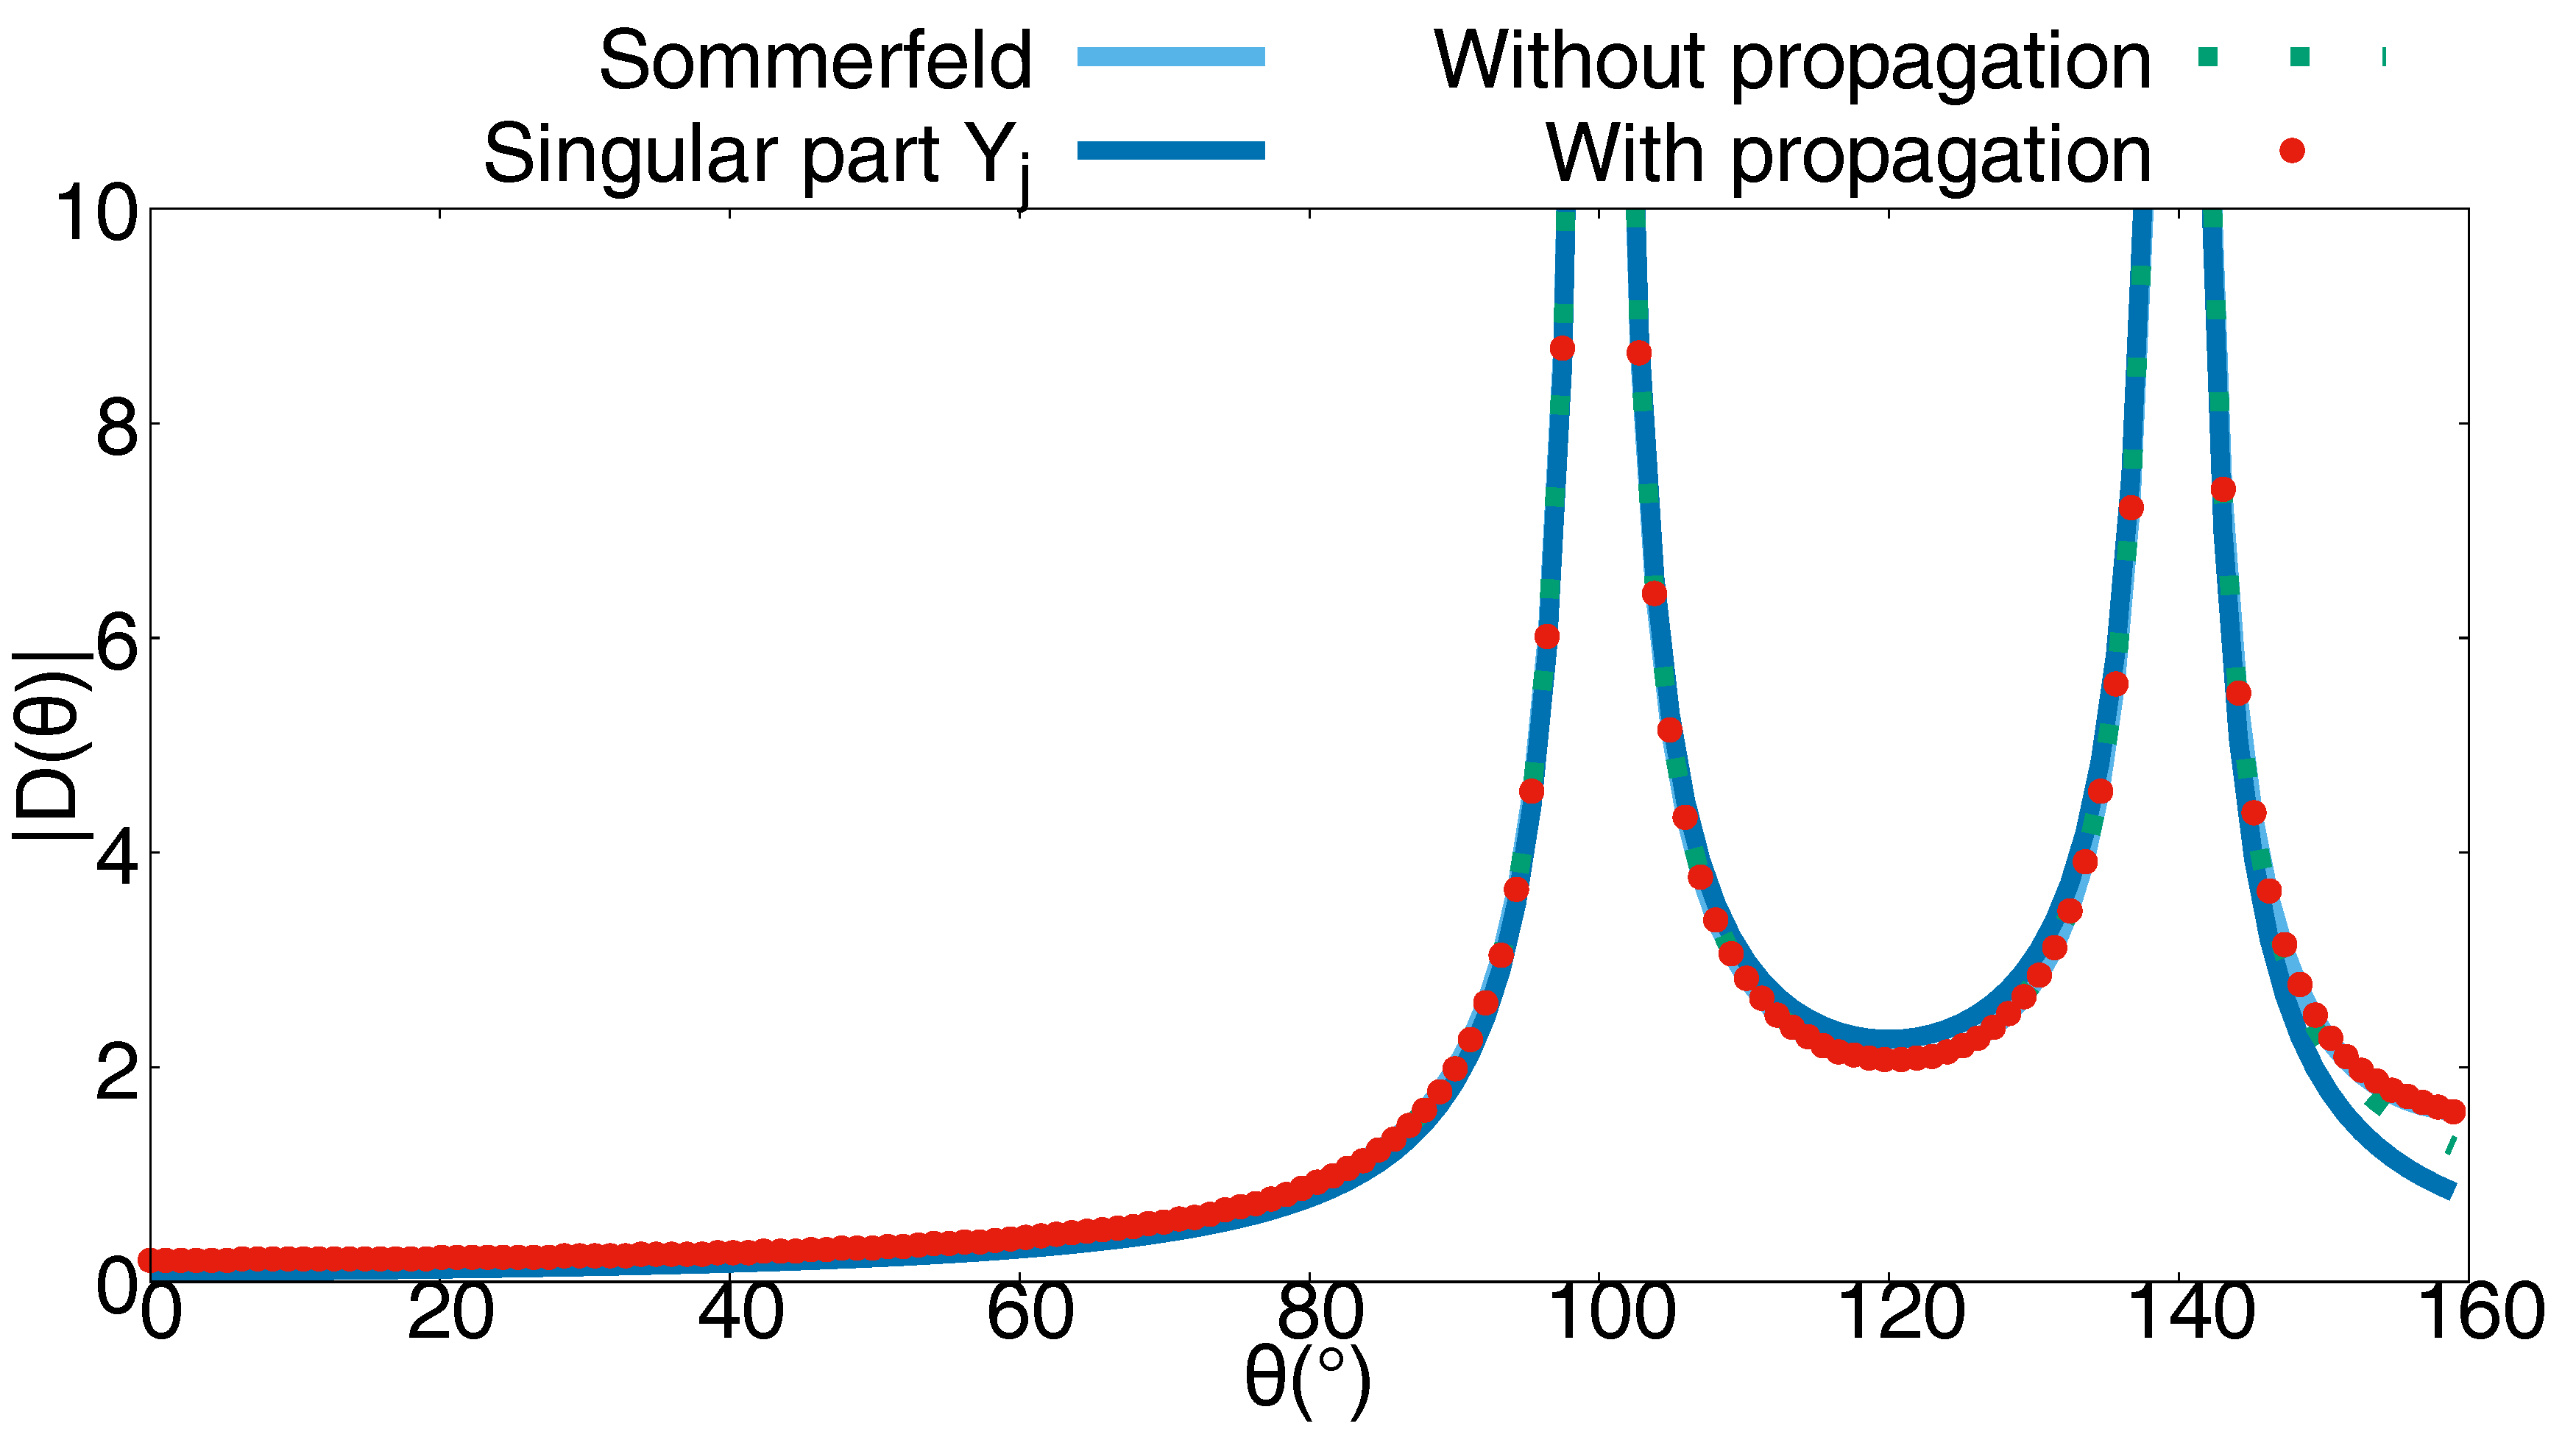
\includegraphics[width=\textwidth]{images/chapter2/Figure9b.pdf}
        \caption{$2\varphi = 160^o$, $\theta_{\rm inc} = 40^o$}
        \label{chapter5:figure13b}
    \end{subfigure}
\\
~\\
\begin{subfigure}[b]{0.49\textwidth}
        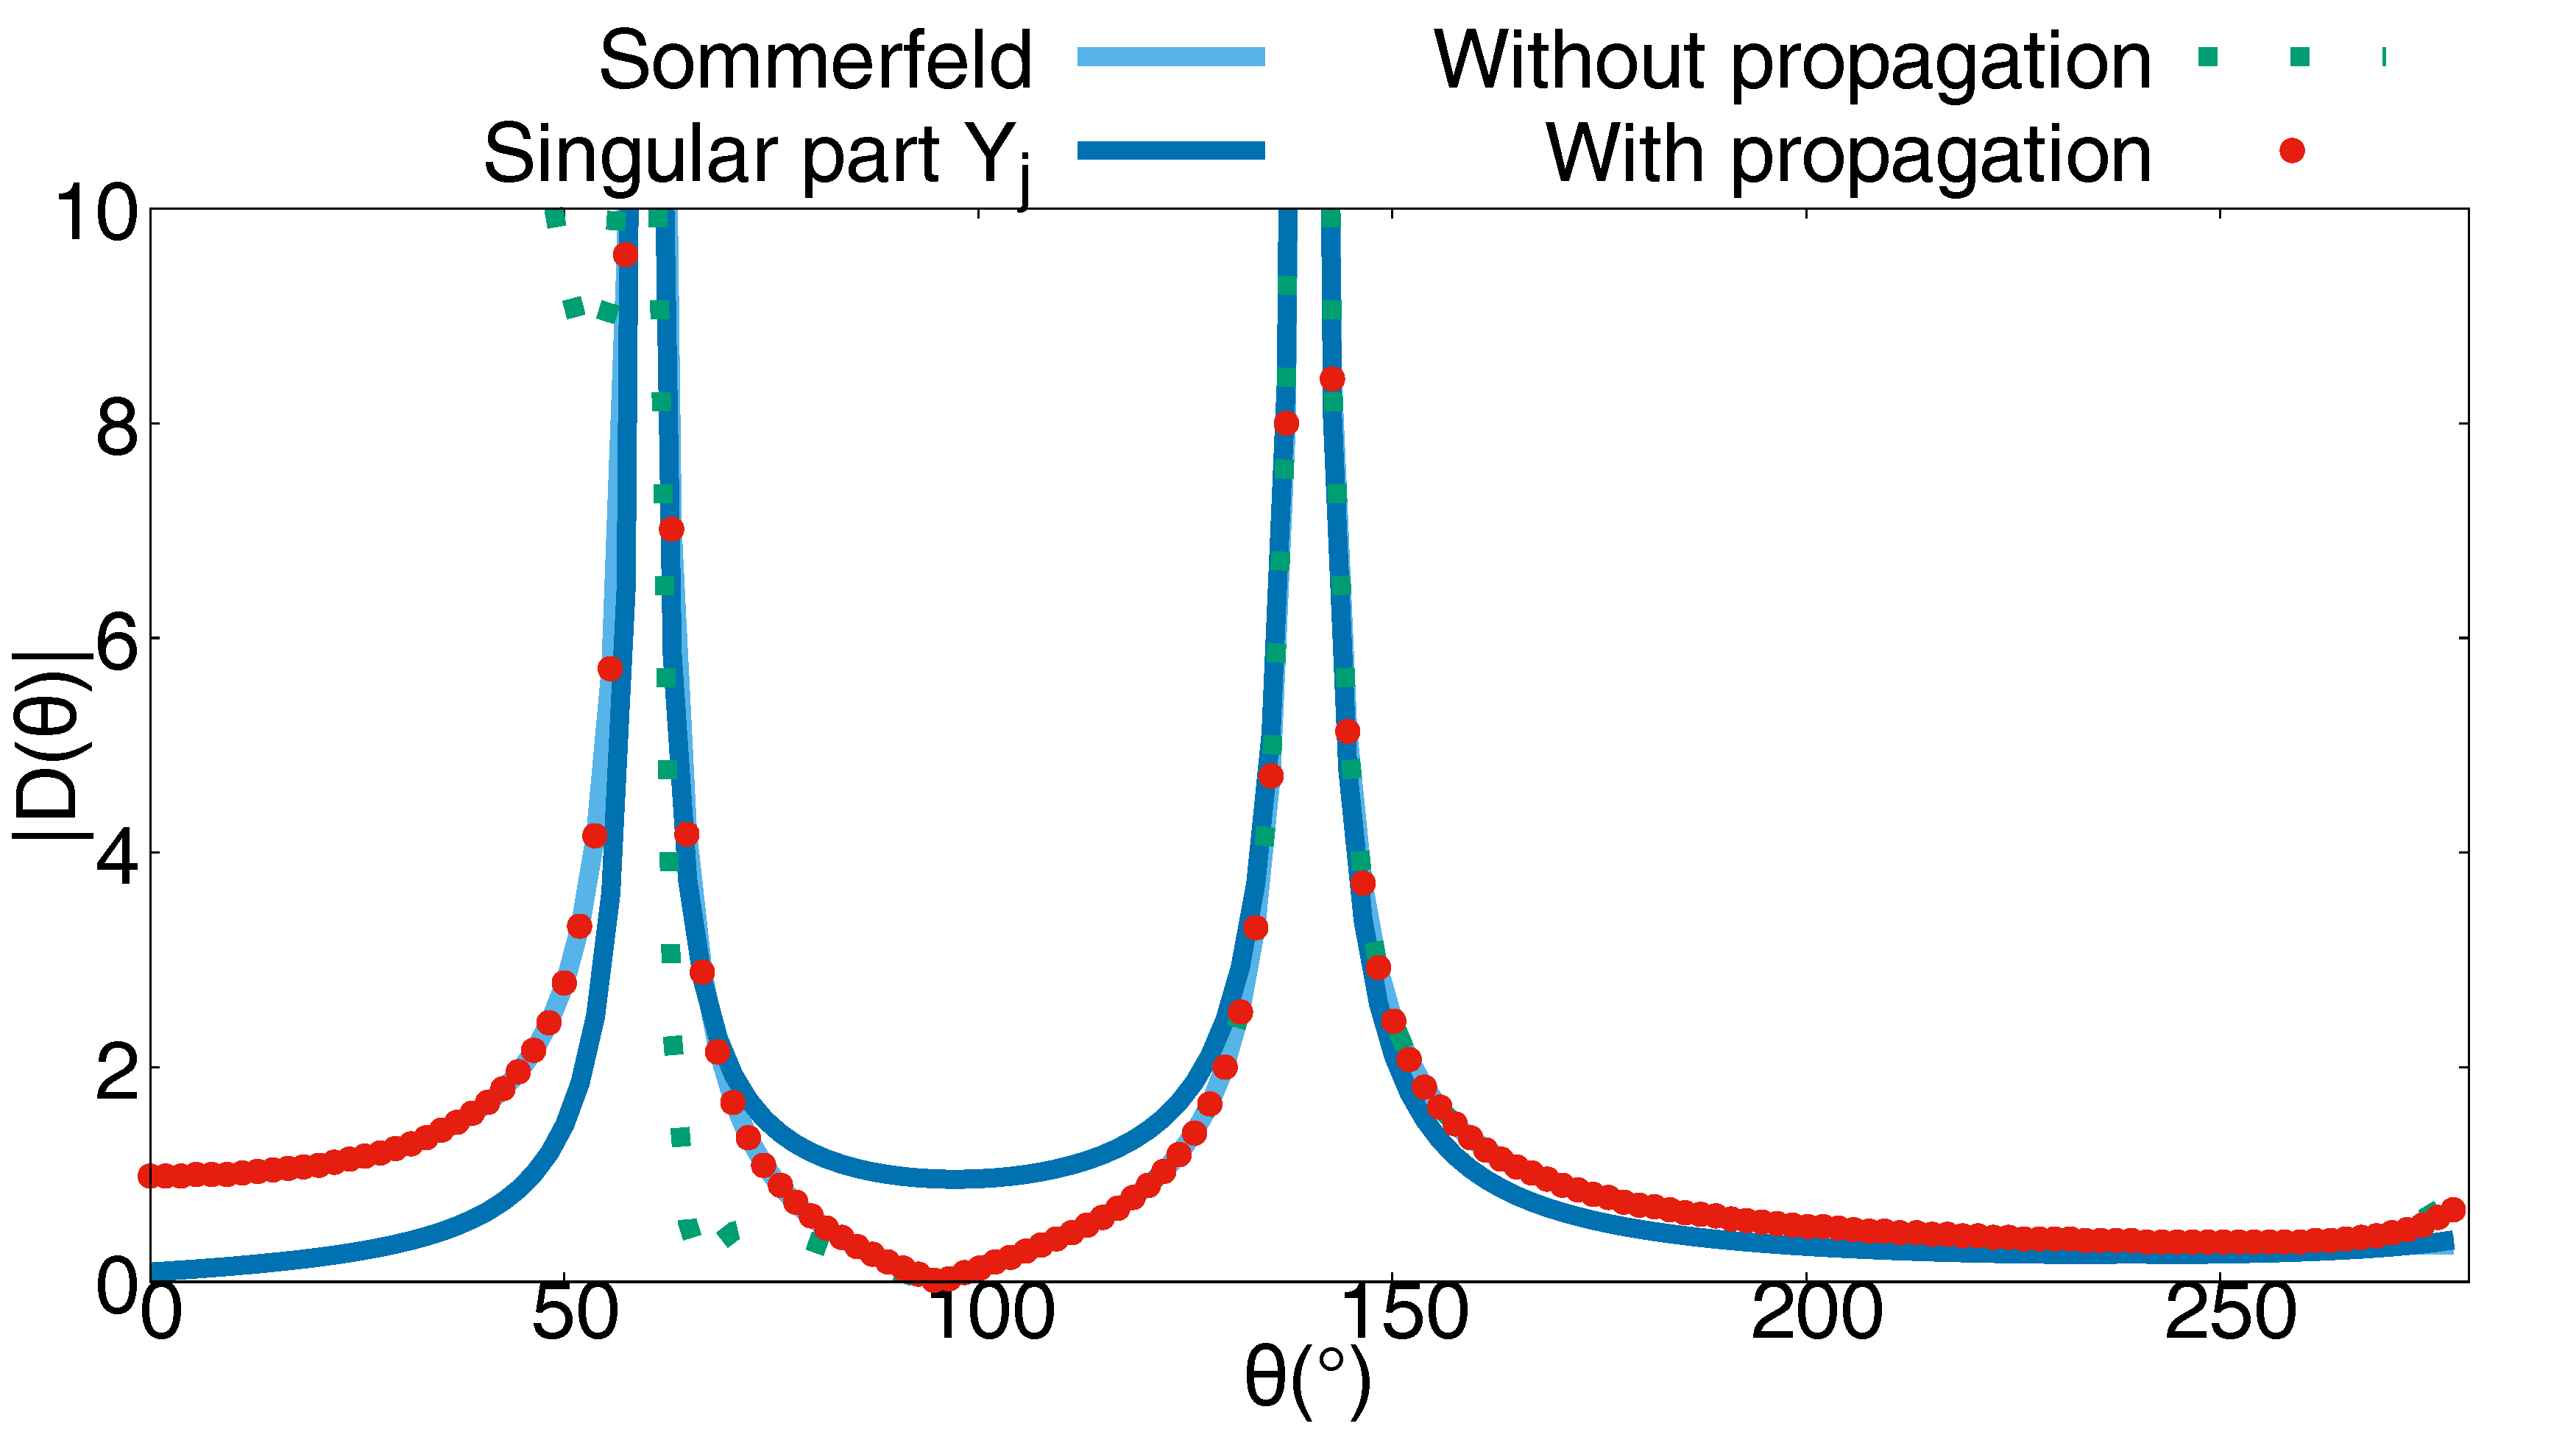
\includegraphics[width=\textwidth]{images/chapter2/Figure9c.pdf}
        \caption{$2\varphi = 280^o$, $\theta_{\rm inc} = 240^o$}
        \label{chapter5:figure13d}
    \end{subfigure}
\begin{subfigure}[b]{0.49\textwidth}
        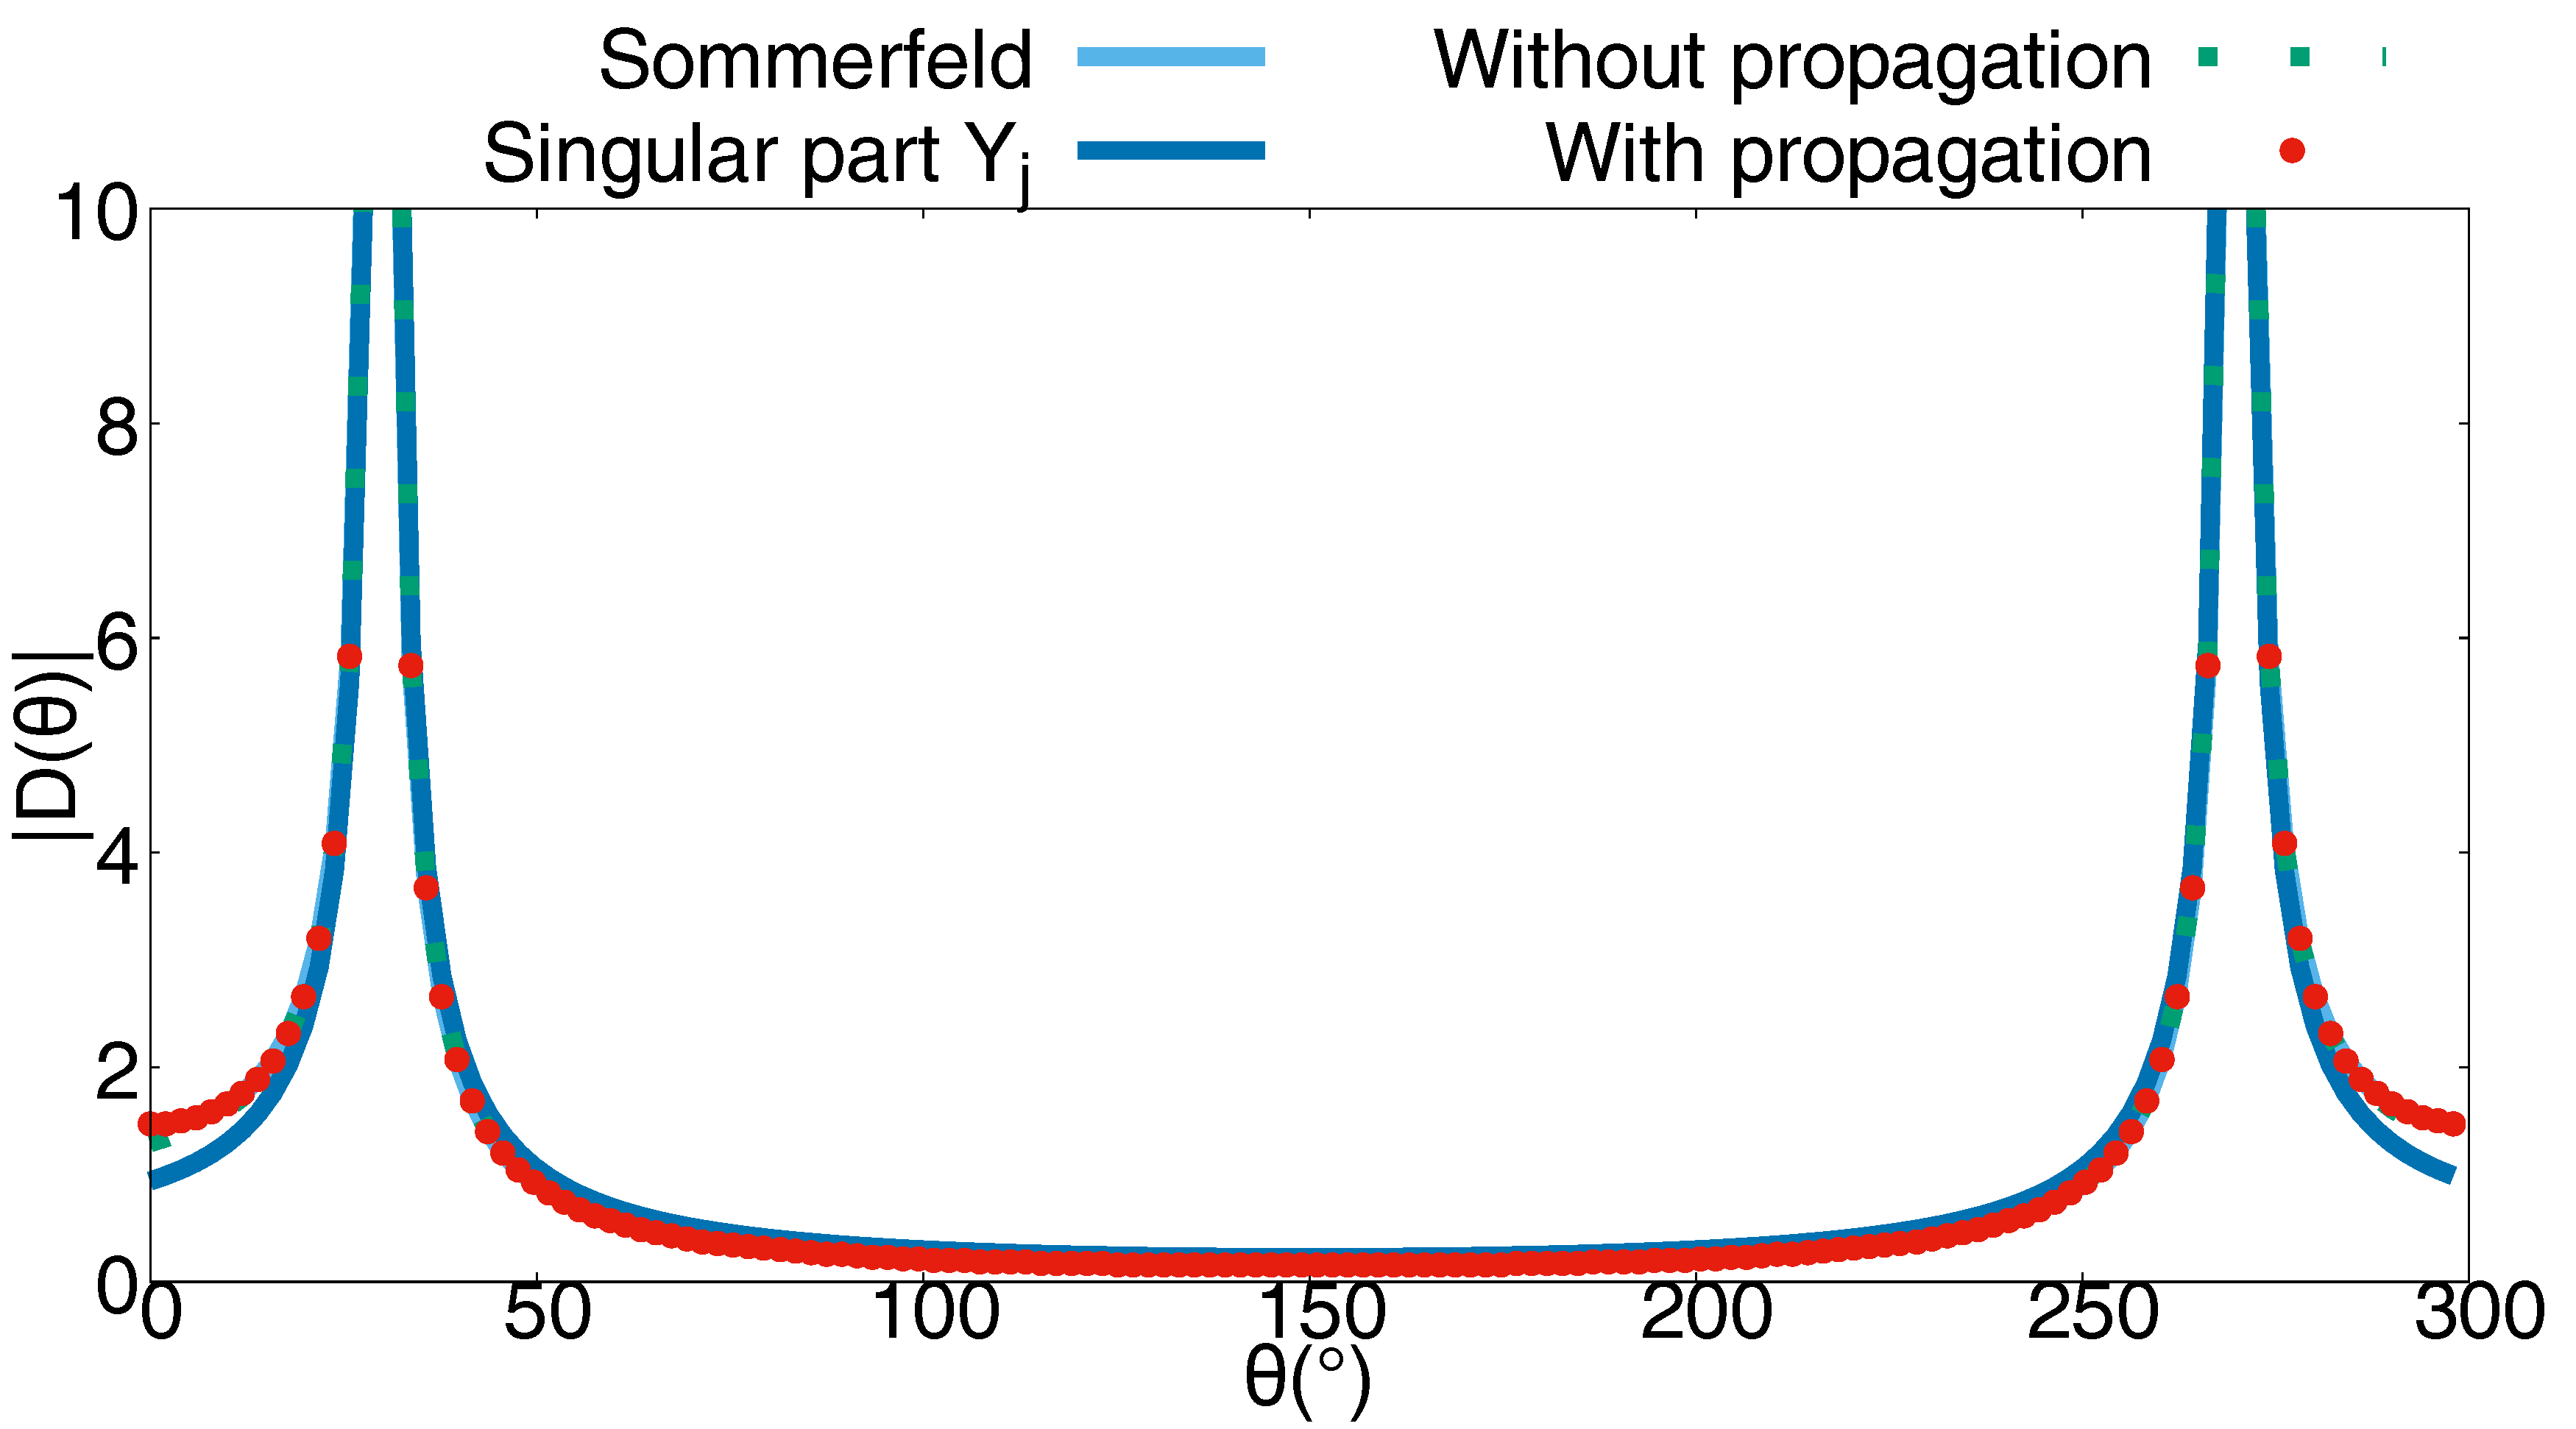
\includegraphics[width=\textwidth]{images/chapter2/Figure9d.pdf}
        \caption{$2\varphi = 300^o$, $\theta_{\rm inc} = 150^o$}
        \label{chapter5:figure13c}
    \end{subfigure}
\caption
[Diffraction  coefficient computed with the recursive formula of spectral functions and with the Sommerfeld method, in the case of Neumann boundary conditions]
{Diffraction  coefficient computed with the spectral functions and with the Sommerfeld method, in the case of Neumann boundary conditions.}
\label{chapter5:figure13}
\end{figure}


 In each of these figures, the continuous light blue line represents the modules of the diffraction coefficients obtained using the Sommerfeld integral method, the continuous dark blue line represents those obtained using the Spectral function singular part $Y_j$ alone, the short-dashed green line represents those obtained using the Spectral functions method without propagation of the solution and the red circles represent those obtained using the spectral functions method with propagation of the solution described in paragraph \ref{propag_sol}.

On Figs.~\ref{chapter5:figure12a},~\ref{chapter5:figure12b},~\ref{chapter5:figure13a} and ~\ref{chapter5:figure13b} the wedge angles are lower than $\pi$ and on figs.~\ref{chapter5:figure12c},~\ref{chapter5:figure12d},~\ref{chapter5:figure13c} and ~\ref{chapter5:figure13d} the wedge angles are greater than $\pi$. In all cases, it appears clearly that both the regular part of the solution and the recursive method are necessary to obtain optimal results. When both of these are included, diffraction coefficients obtained with Spectral functions are close to those of the Sommerfeld method. In addition, the run time to evaluate the diffraction coefficients in 250 different observation points, in each of the presented configurations, using an Intel(R) Xeon(R) CPU E3-1240 v3 is under 0.1 seconds for both methods. 
%
% Deuxième chapitre

\chapter[][Acoustic Case]{The spectral functions method for acoustic wave diffraction by a stress-free
wedge : theory and validation}
\label{chap-developpement}


\section{Introduction}
The canonical problem of an acoustic, electromagnetic or elastodynamic plane wave diffraction by a wedge with Neumann or Dirichlet boundary conditions is a complex mathematical problem which has been of great interest to researchers for over a century.

The mathematical theory of wedge diffraction was first introduced by Sommerfeld \cite{Sommerfeld}, who gave an analytical expression of the exact solution of the diffraction problem of a scalar plane wave as a contour integral \cite{SMtechnique}. Macdonald \cite{Macdo} has expressed the scalar solution as a series, using the variables separation technique. Sommerfeld \cite{Sommerfeld} gave an analytical formula of the \acrfull{gtd} diffraction coefficient for an arbitrary-angled wedge (with Neumann or Dirichlet boundary conditions) illuminated by a scalar plane wave. This wedge \acrshort{gtd} coefficient can be used for scalar wave diffraction both in electromagnetics \cite{Kouyoumjian} and in acoustics \cite{Bouche,Bo}.

%In the more complex case of an elastic wave diffracted by a wedge of angle less than $\pi$, there exist two major approaches : one is based on the Sommerfeld integral (SI) representation of the elastodynamic potentials, it was introduced by Budaev and Bogy \cite{Rayleigh} and clarified by Kamotski et al. \cite{KamotskiFradkin}. The other method is based on the Laplace transform of the displacement field (LT), and was developed by Gautesen and Fradkin \cite{GautesenFradkin}. In the particular case of a scattered Rayleigh wave, a method which uses the free-space Green's tensor to express the Fourier transform of the displacement field has been developed by Gautesen for wedge angles smaller and greater than $\pi$ \cite{GautesenRayleigh,GautesenRayleigh2}. However the range of the wedge angle was restricted to the range $\lbrack 63^o,180^o\rbrack $ for angles smaller than $\pi$ and to $\lbrack 189^o,327^o \rbrack$ for angles greater than $\pi$ in order to avoid numerical instabilities.
%
%These methods are non-uniform in the sense that they lead to a solution which diverges at shadow boundaries and caustics of the Geometric-Elastic (GE) field \cite{Bouche}. To overcome this difficulty, Ufimtsev \cite{Ufmi} has introduced the Physical Theory of Diffraction (PTD) in electromagnetics. This technique has been extended to elastic waves by Zernov et al. \cite{Zernov}, however it is computationally expensive. 
%Another uniform correction of GTD is the Uniform Asymptotic Theory (UAT), introduced by Lewis \cite{Lewis} in electromagnetics and acoustics and extended to elastodynamics by Achenbach et al. \cite{Achenbach}, which gives a systematic approach for computing a uniform solution but is quite complicated to implement for complex geometries as it requires extension of the reflected field to its shadow zone using fictitious rays \cite{Bouche}, \cite{Molinet}.
%For practical purposes, the most used uniform correction of the GTD method is the Uniform Theory of Diffraction (UTD) as it is computationally efficient and does not require an artificial extension of the reflected field. It was developed in electromagnetics by Kouyoumjian and Pathak \cite{Kouyoumjian}, using the Pauli-Clemmow method \cite{Pauli} and extended to elastodynamics by Kamta Djakou et al. \cite{Audrey}. A comparison of different asymptotic (GTD and uniform) and exact solutions has been carried out in elastodynamics by Aristizabal et al. \cite{Aristizabal} but for the scalar case of the 2D wedge diffraction of a shear horizontally polarized incident wave.

%For a certain time, methods of computation have been studied without proof of solvability for the wedge diffraction problem. Osher \cite{Osher1, Osher2} has studied the well-posedness of hyperbolic initial and boundary value problems (meaning the solution is fixed at $t=0$ and on the domain boundaries) in a region with a corner (meaning a right-angled wedge) and has given certain necessary conditions that the boundary values must verify in order for a problem to be well-posed; he has thoroughly presented the consequences if these conditions were not verified. Huang and Temam \cite{Huang} have studied the well-posedness of hyperbolic initial and boundary value problems in a rectangular domain and have also specified how the boundary values must be chosen for the problem to be solvable; they have also given a brief explanation as to how their theory can be applied to wave equations.

These methods of computation have been proposed without proof of solvability for the wedge diffraction problem. Castro and Kapanadze \cite{Castro} have proven existence and uniqueness of the solution for acoustic and electromagnetic plane waves using a detailed Fredholm analysis. Kamotski and Lebeau \cite{KamotskiLebeau} have proven existence and uniqueness of the solution to the elastic plane wave diffraction  by a soft wedge (Dirichlet boundary) problem using the Spectral Functions method in which the diffracted wave is modeled thanks to these spectral functions. Their demonstration is valid for all wedge angles but they do not propose any method of computation of the solution. The Spectral Functions method was at first developed by Croisille and Lebeau \cite{CroisilleLebeau} who proposed a numerical algorithm in order to compute these functions for elastic wedges of angle lower than $\pi$ immersed in a fluid. In this chapter, wedges of any angle (even larger than $\pi$) are taken into account, and the outside medium is void. There is only one wave type to be considered and Dirichlet or Neumann boundary conditions are supposed, as opposed to the case studied by Croisille and Lebeau \cite{CroisilleLebeau} where three propagation modes coupled by the boundary conditions are considered, but only for wedge angles lower than $\pi$.

In the field of seismic diffraction, other approaches have been developed. The problem of acoustic diffraction in a system of wedge-shaped regions was studied by Klem-Musatov \cite{Klem-Musatov}. Using the Malyuzhinetz transform, this problem is reduced to a system of functional equations. However, this system is too complex to be solved in general cases. A successive approximations method is proposed in the particular case of a wedge-shaped separation between two media having the same acoustic wave velocity or  in the case where the medium containing the incident wave is a wedge of angle lower than $\pi$. In the very general case of acoustic wave propagation in a homogeneous or inhomogeneous medium delimited by an arbitrary-shaped boundary, a mathematical model has been rigorously presented by Aizenberg and Ayzenberg \cite{Aizenberg}, providing the analytical feasible fundamental solution for this problem. The notion of feasible fundamental solution is a generalization of Green's function for an unbounded medium. Ayzenberg \cite{Ayzenberg} shows how this general mathematical model can be numerically applied to the case of wedge diffraction. This method is applied in the case of a spherical source and it appears that parallel computation is necessary to obtain a short computation time, whereas the spectral functions method is applied here in the case of plane-wave diffraction and a simple architecture is sufficient to obtain results for a short computation time. 

The aim of this chapter is to develop and implement the methodology of Croisille and Lebeau \cite{CroisilleLebeau} in the two-dimensional (i.e. the incident wave vector lies in the plane normal to the edge) case of an acoustic wave diffracted by a soft wedge immersed in a fluid (Dirichlet boundary condition) and propose a numerical validation of the method for angles both smaller and larger than $\pi$.  The expansion to all wedge angles is obtained using Kamotski and Lebeau's \cite{KamotskiLebeau} idea of defining a new angular variable, $\widetilde{2\varphi}$, defined in equation \eqref{phitilde}, thanks to which the complete resolution and the computation of the solution are proposed and developed here for all wedge angles with a single method. Numerical validation will be achieved by comparing the GTD approximation of the diffraction coefficient obtained using the spectral functions method, with the analytical expression given in \cite{Bouche,Bo} of the GTD approximation of the exact solution. 

The outline of the chapter is the following: section \ref{Chapter5:problem}. presents the problem and the diffraction coefficients are expressed in terms of the spectral functions. The resolution of the problem is discussed in section \ref{Chapter5:resolution}. Finally, numerical results are given in section \ref{Chapter5:results}. and compared to the analytical Sommerfeld solution. 

\section{Problem statement}
\label{Chapter5:problem}

Let us consider a stress-free wedge of angle $\varphi$ immersed in a fluid $\Omega_f$ constituted of the junction of two faces $\mathcal{S}_1$ and $\mathcal{S}_2$ (see Fig.~\ref{chapter5:figure1}). The inward unit vectors normal to each of these faces are noted $n_1$ and $n_2$ respectively. The Cartesian coordinate system $(O; \mathbf{e}_{x_1}, \mathbf{e}_{y_1} )$ is linked to the face $\mathcal{S}_1$ of the wedge and $(O;  \mathbf{e}_{x_2}, \mathbf{e}_{y_2} )$ is linked to the face $\mathcal{S}_2$. These Cartesian coordinate systems  have the same origin located on the wedge edge which coincides with the $z$-axis. Let $\mathbf{x} = (x_1,y_1)_{ (\mathbf{e}_{x_1}, \mathbf{e}_{y_1}) } = (x_2,y_2)_{ (\mathbf{e}_{x_2}, \mathbf{e}_{y_2})}$ be a position vector $\mathbf{x} = (r,0)$ in a local basis of polar coordinates associated to the Cartesian coordinates $(x_1,y_1)$. The time convention used in this chapter is $\exp(i\omega t)$. The wedge is thus irradiated by a velocity potential plane wave in the form
\begin{align}
\label{Chapter5:incidence_wave}
g^{\rm inc}(\mathbf{x},t) = A \, e^{i(\omega t - \mathbf{k}^{\rm inc} \cdot \mathbf{x})}
\end{align}

where $A$ is the amplitude of the incident velocity potential, $\omega$ is the circular frequency, $t$ is time and 
\begin{align}
\mathbf{k}^{\rm inc} = k_0 (-\cos \theta_{\rm inc},-\sin \theta_{\rm inc})_{(\mathbf{e}_{x_1}, \mathbf{e}_{y_1})}
\end{align}
is the wave vector of the incident wave with $k_0 = \omega/c_0$ being the wave number and $c_0$ is the sound velocity in the fluid.  The velocity potential in the fluid $g$ satisfies the motion equation in the fluid medium $\Omega_f$ surrounding the wedge 
\begin{equation}
\label{Chapter5:WaveMotion}
\frac{\partial^2 g}{\partial t^2} - c_0^2 \, \triangle g = 0
\end{equation}
and the boundary condition on the wedges faces
\begin{equation}
\label{Chapter5:CL}
Bg\mid_{\mathcal{S}_j} = 0, \quad j=1,2,
\end{equation}
where the expression of operator B is given by \eqref{Chapter5:CLDir} for Dirichlet boundary conditions and by \eqref{Chapter5:CLNeu} for Neumann boundary conditoins :
\begin{subequations}
\begin{equation}
\label{Chapter5:CLDir}
Bg = g \quad \mbox{for Dirichlet boundary conditons}
\end{equation}
\begin{equation}
\label{Chapter5:CLNeu}
Bg = \frac{\partial g}{\partial n} \quad \mbox{for Neumann boundary conditons}
\end{equation}
\end{subequations}

This common notation makes it possible to treat both cases simultaneously in the following developments.

\begin{figure}[h]
\centering
	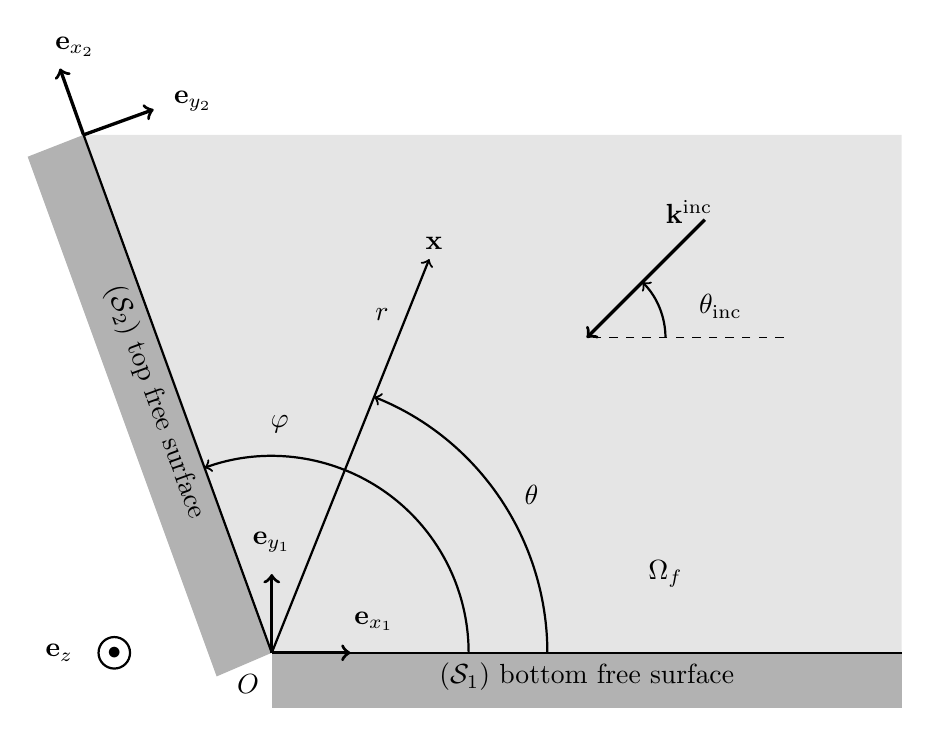
\begin{tikzpicture}
	\fill[color=gray!20] (0,0) -- (8,0)  -- (8,6.5778) -- (-2.39,6.5778) -- cycle;  
	\draw[ thick, ->] (2.5,0) arc (0:110:2.5);
	
	\fill[color=gray!60] (0,0) -- (8,0)  -- (8,-0.7) -- (0,-0.7) -- cycle;  
	
	\fill[color=gray!60] (0,0) --  (-2.39,6.5778) --(-3.1,6.3) -- (-0.7,-0.3) -- cycle; 
		
	\draw[thick, color = black]  (0,0) -- (8,0) node[midway,below] {($\mathcal{S}_1$) bottom free surface};
	
	\draw[thick, color = black]  (0,0) -- (-2.39,6.5778) node[midway,below,sloped] {($\mathcal{S}_2$) top free surface};
	
	\draw[very thick, ->] (-2.39,6.5778) -- (-2.69,7.42);
	
	\node[scale=1] at (-2.5,7.7){$\mathbf{e}_{x_2}$};
	
	\draw[very thick, ->] (-2.39,6.5778) -- (-1.5,6.9);
	
	\node at (-1,7){$\mathbf{e}_{y_2} $};
	
	
	\node at (0.1,2.9){$\varphi$} ; 
	
	\draw[very thick, ->] (0,0) -- (1,0);
	
	\node at (1.3,0.4) {$\mathbf{e}_{x_1} $};
	
	\draw[very thick, ->] (0,0) -- (0,1);
	
	\node at (0,1.4){$\mathbf{e}_{y_1} $};
	
	\node at (-2,-0.01) {$\bullet$};
	
	\draw[thick] (-2,0) circle (0.2);
	
	\node at (-2.7,0){$\mathbf{e}_{z}$};
	
	\draw[very thick, ->] (5.5,5.5) -- (4,4);
	
	\draw[dashed] (6.5,4) -- (4,4);
	
	\draw[thick, ->] (5,4) arc (0:45:1);
	
	\node at (5.7,4.4){$\theta_{\rm inc}$};
	
	\node at (5.3,5.6){ $\mathbf{k}^{\rm inc}$};
	
	\node at (-0.3,-0.4){ $O$};
	
	\node at (5,1){$\Omega_f$ };
	
	% point observation
	
	\draw[thick, ->] (0,0) -- (2,5); 
	
	\draw[thick, ->] (3.5,0) arc (0:68.2:3.5);
	
	\node at (3.3,2){$\theta$};
	
	\node at (1.4,4.3){$r$};
	
	\node at (2.06,5.2){$\mathbf{x}$};
	
	\end{tikzpicture}
	\caption
[Geometry of the problem]
{The wedge of angle $2\varphi$ whose faces are stress-free is illuminated by a plane wave of wave vector $\mathbf{k}^{\rm inc}$.}
\label{chapter5:figure1}
\end{figure}
The dimensionless form of the problem is obtained  by defining the function $h$ by
\begin{equation}
\label{Chapter5:dimensionless}
g(\mathbf{x},t) = 2A \, e^{i \omega t} \, h(k_0 \mathbf{x}).  
\end{equation}

The dimensionless function $h$ is the sum of the  incident dimensionless  wave $h_{inc}$ and of the scattered dimensionless  wave $v$
\begin{equation}
h = h_{inc} + v
\label{decompinc}
\end{equation}
In this decomposition, the scattered wave $v$ is the sum of two fields : the Geometric-Elastodynamic (GE) field, which  is the sum of the possibly multiple specular reflections of the incident wave and of fictitious fields compensating the incident wave in shadow zones, and the diffracted field. A detailed description of the GE field, in the case of a half-plane scatterer, is given by Kamta-Djakou et al. \cite{Audrey}.

The system \eqref{Chapter5:WaveMotion}-\eqref{Chapter5:CL} is equivalent to the following  system of equations for the dimensionless problem, obtained by inserting Fourier transform \eqref{Chapter5:dimensionless} and decomposition \eqref{decompinc} into equations \eqref{Chapter5:WaveMotion} and \eqref{Chapter5:CL}
\begin{equation}
\label{Chapter5:Adimen_waveMotion}
\begin{cases}
(\triangle+1)v =  0 \quad \text{in } \Omega_f, \\
Bv =  -Bh_{inc} \quad \quad \quad \text{on } \mathcal{S}_j, \quad j=1,2
\end{cases}.
\end{equation}

In order to obtain a solution to this problem which is physically relevant, the limiting absorption principle is used. It consists in substituting the wave number $k_0$ by a complex one $k_0 e^{-i\epsilon} $ with $\epsilon > 0$. This means that absorption occurs in the medium and thus the scattered waves attenuate with the distance. The system (\ref{Chapter5:Adimen_waveMotion}) then becomes :
\begin{equation}
\label{Chapter5:waveMotion_epsilon}
(S_\epsilon^*) \quad
\begin{cases}
(\triangle+ \, e^{-2i\epsilon}) v^\epsilon  =  0 \quad \text{in } \Omega_f, \\
Bv^\epsilon  =  -Bh_{\rm inc}^\epsilon  \quad \text{on } \mathcal{S}_j, \quad j=1,2
\end{cases}
\end{equation}

The physically relevant solution to (\ref{Chapter5:Adimen_waveMotion}), called the outgoing solution, can now be defined. It is the one obtained when taking $\epsilon \to 0$ in (\ref{Chapter5:waveMotion_epsilon}). This limit is noted $v^0$. Its integral representation is found hereafter.

\subsection*{Outgoing solution: integral representation}
\label{integral_representation}

First, a special class of distributions is defined.
\begin{definition}
The class of distributions $\mathcal{A}$ is defined as follows. The distribution $f\in \mathcal{A}$ if :
\begin{itemize}
\item $f \in \mathcal{L}^2(\mathbb{R})$ (f is a tempered distribution)
\item supp$(f) \subset \lbrack 0,+\infty \lbrack$
\item $\exists C_0>0$ such that
$$ \sup_{-\pi<\theta<0} \int_{\rho>C_0}|\hat{f}(\rho e^{i\theta})|^2\,d\rho <\infty$$
where $\hat{f}$ is the Fourier transform of $f$ defined by $\hat{f}(\xi)=\int_{\mathbb{R}}f(x)e^{-ix\xi}\, dx$.
\item $\hat{f}(\xi)$ is holomorphic near $\xi=1$
\end{itemize}

\end{definition}
The outgoing solution to (\ref{Chapter5:Adimen_waveMotion}) can now be defined properly.

\begin{definition}
An outgoing solution of the equation (\ref{Chapter5:Adimen_waveMotion}) is a solution v of the form 
\begin{equation}
\label{Chapter5:decomposition}
v=v_1|_{\Omega_f}+v_2|_{\Omega_f}
\end{equation}
where, for $j=1,2$ :
\begin{equation}
\label{inv_potentiels}
v_j=-\lim_{\epsilon \to 0} \left(\Delta+e^{-2i\epsilon}\right)^{-1} \left[ \alpha_j \otimes \delta_{\mathcal{S}_j} \right]
\end{equation}
$\alpha_j \in \mathcal{A}$ are unknown and $\delta_{\mathcal{S}_1}$ and $\delta_{\mathcal{S}_2}$ are the Dirac delta functions on the faces $\mathcal{S}_1$ and $\mathcal{S}_2$ of the wedge respectively (these functions verify $\delta_{\mathcal{S}_j}(x,y)=1$ on $\mathcal{S}_j$, and $\delta_{\mathcal{S}_j}(x,y)=0$ elsewhere).

\end{definition}
The following theorem is proven by Croisille and Lebeau in \cite{CroisilleLebeau} :
\begin{theorem}
The equation \eqref{Chapter5:Adimen_waveMotion} admits a unique outgoing solution.
\end{theorem}

The aim of this chapter is to extend and detail the computation of this outgoing solution for the stress-free wedge immersed in a fluid using the spectral functions method.

The double Fourier transform of a tempered distribution and its inverse are defined by :
\begin{subequations}
\begin{equation}
\hat{f}(\xi,\eta)=\int \int_{\mathbb{R}^2}f(x,y)e^{-i(x\xi+y\eta)}\, {\rm d}x {\rm d}y
\label{fourierdef}
\end{equation}
\begin{equation}
f(x,y)=\frac{1}{4\pi^2}\int\int_{\mathbb{R}^2} \hat{f}(\xi,\eta)e^{i(x\xi+y\eta)}\rm d\xi \rm d\eta
\label{invfourierdef}
\end{equation}
\label{fullfourierdef}
\end{subequations}

The double Fourier transform of (\ref{inv_potentiels}) using \eqref{fourierdef} gives
\begin{equation}
\label{Fourier}
\hat{v_j^\epsilon} =  \left[ \xi^2 + \eta^2 - e^{-2i\epsilon} \right]^{-1} \hat{\alpha_j}.
\end{equation}

 The dimensionless velocity potential $v_j^\epsilon$ is then found by applying the inverse Fourier transform in $\xi$ and $\eta$ to \eqref{Fourier}. 
\begin{equation}
\label{velocity_inv_fourier2}
v_j^\epsilon = \dfrac{1}{4\pi^2}  \int_{-\infty}^{+\infty}\left( \int_{-\infty}^{+\infty} \dfrac{e^{iy_j\eta}}{ \xi^2 + \eta^2 - e^{-2i\epsilon}} {\rm d}\eta \right)\,  \hat{\alpha_j}(\xi) \,  e^{i x_j \xi}  {\rm d} \xi.
\end{equation}

For  $\epsilon \neq 0$, the inner integrand poles are given by
\begin{equation}
 \eta = \pm \sqrt{e^{-2i\epsilon} - \xi^2}  = \pm \zeta_0^\epsilon
\end{equation} 
and are never crossed by integration along the real axis. Integral \eqref{velocity_inv_fourier2} can be calculated using the residue theorem which leads to the following result
\begin{equation}
\label{champ_epsilon}
v_j^\epsilon(x_j,y_j) = \dfrac{i}{4\pi} \int_{-\infty}^{+\infty}  \dfrac{e^{i|y_j|\zeta_0^\epsilon(\xi)} e^{i x_j \xi}}{\zeta_0^\epsilon(\xi)} \hat{\alpha_j}(\xi) \, {\rm d}\xi.
\end{equation}
This integral is well defined if $\text{Im}(\zeta_0^\epsilon) > 0$, so that the exponential in the integral decreases with the distance $y_j$ and the absorption principle is respected. Function $\zeta_0^\epsilon(\xi)$ then satisfies for $\xi$ real
\begin{subequations}
\label{zeta_function}
\begin{align}
\zeta_0^\epsilon(\xi)&= i\sqrt{\xi^2-e^{-i\epsilon}} \quad \text{if} \quad \vert \xi\vert \geq 1,\\
\label{zeta_function_inferior1}
\zeta_0^\epsilon(\xi)&= -\sqrt{e^{-i\epsilon}-\xi^2} \quad  \text{if} \quad \vert \xi\vert \leq 1.
\end{align}
\end{subequations}
The branch points of the function $\zeta_0^\epsilon(\xi)$ are $\pm  \, e^{-i\epsilon}$. For $\epsilon > 0$, integral \eqref{champ_epsilon} is well defined because these complex singular points are never crossed by the integration contour (the real axis). The integration contour of \eqref{champ_epsilon}, is deformed into the contour $\Gamma_0$ illustrated on Fig.~\ref{chapter5:figure2} so that these singular points $\pm  \, e^{-i\epsilon}$ are not crossed by the new contour $\Gamma_0$  when $\epsilon \rightarrow 0$ (for which the physical outgoing solution of (\ref{Chapter5:waveMotion_epsilon}) is obtained). The curved arrows on Fig.~\ref{chapter5:figure2} are described later in section \ref{Chapter5:regular_part}.

Thus, even for $\epsilon=0$, the integral
\begin{equation}
\label{champ}
v_j^0(x_j,y_j) = \dfrac{i}{4\pi} \int_{\Gamma_0}  \dfrac{e^{i|y_j|\zeta_0^0(\xi)} e^{i x_j \xi}}{\zeta_0^0(\xi)} \hat{\alpha_j}(\xi)  \, {\rm d}\xi
\end{equation}
converges.
Using \eqref{Chapter5:decomposition}, our initial solution is then
\begin{equation}
\label{initial_sol}
v(\mathbf{x}) = v_1^0(x_1,y_1) + v_2^0(x_2,y_2)
\end{equation}

\begin{figure}[ht]%
	\centering
	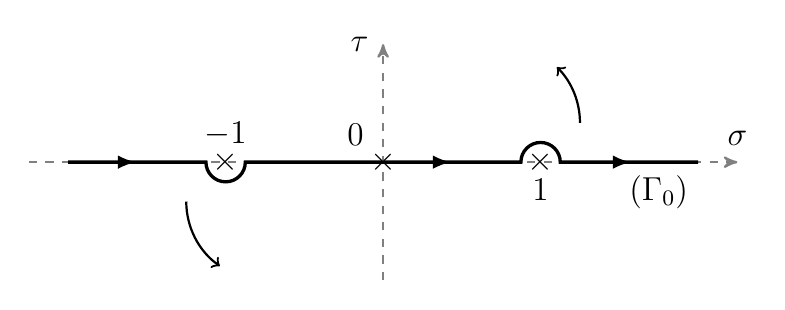
\begin{tikzpicture}
	\node at (0,0) {\large $\times$};
	\node at (-0.35,0.35) {\large $0$};
	\node at (2,0) {\large $\times$}; % Pole
	\node at (2,-0.35) {\large $1$};
	\node at (-2,0) {\large $\times$};
	\node at (-2,0.35) {\large $-1$}; %pole
	\node at (3.5,-0.38) {\large $(\Gamma_0)$};
	\draw[ thick, ->] (-2.5,-0.5) arc (180:235:1);
%	\node at (-2.8,-0.9) {\large $\mathcal{F}_1$};
	\draw[ thick, ->] (2.5,0.5) arc (0:45:1); %ici c'est les fleches 
	%\node at (2.8,0.9) {\large $\mathcal{F}_2$};
    \node at (4.5,0.3) {\large $\sigma$};
    \node at (-0.3,1.5) {\large $\tau$};
	\draw[step=1.5cm,gray,thick,dashed,->,>=stealth'] (-4.5,0) -- (4.5,0);
	\draw[step=1.5cm,gray,thick,dashed,->,>=stealth'] (0,-1.5) -- (0,1.5);
	\draw[very thick,black,yshift=0pt,
	decoration={ markings,  % This schema allows for fine-tuning the positions of arrows 
		mark=at position 0.1 with {\arrow{latex}},
		mark=at position 0.6 with {\arrow{latex}},
		mark=at position 0.9 with {\arrow{latex}}},
	postaction={decorate}]
	(-4,0)  -- (-2.25,0)  arc (-180:0:0.25)  -- (1.75,0)arc (180:0:0.25)  --  (4,0); % ca c'est l'axe
	\end{tikzpicture}
\caption
[Contour $\Gamma_0$]
{Integration contour $\Gamma_0$ in the complex plane $\xi = \sigma + i \tau$. The curved arrows show the deformation of $\Gamma_0$ into the imaginary axis.}
\label{chapter5:figure2}
\end{figure}

One of the goals of this chapter is to compute the spectral functions $\hat{\alpha}_1(\xi)$ and $\hat{\alpha}_2(\xi)$ in order to find the GTD diffraction coefficient \eqref{GTDCoeff_SF}. The accuracy of the spectral functions method is evaluated in section 4 by comparing results of \eqref{GTDCoeff_SF} with \eqref{GTDCoeff_Dir} in the case of Dirichlet boundary conditions and \eqref{GTDCoeff_Neu} in the case of Neumann boundary conditions. Section \ref{Chapter5:resolution} is devoted to the computation of the spectral functions $\hat{\alpha}_1$ and $\hat{\alpha}_2$.


\section{Spectral functions computation}
\label{Chapter5:resolution}

To compute the spectral functions, the functional equations satisfied by these spectral functions $\hat{\alpha}_1$ and $\hat{\alpha}_2$ first have to be determined.
\subsection{Functional equations of spectral functions}

The velocity potential in the boundary conditions of the system \eqref{Chapter5:waveMotion_epsilon} is substituted by its expression \eqref{initial_sol}. It then leads to the following system of equations for the boundary conditions on each wedge face:
\begin{equation}
\label{CL}
\begin{cases}
Bv_1^0(x_1,0) + Bv_2^0(x_2 \cos \varphi,x_2 \sin \varphi)  =  -Bv^0_{\rm inc} \mid_{\mathcal{S}_1}\\
Bv_1^0(x_1 \cos \varphi,x_1 \sin \varphi) + Bv_2^0(x_2,0)   =  -Bv^0_{\rm inc} \mid_{\mathcal{S}_2}
\end{cases}.
\end{equation}
The Fourier transform is applied to the potential velocity expression on the face of each wedge
\begin{align}
\mathcal{F}(x_j \mapsto v_j^0 (x_j,0))(\xi) & =  \dfrac{i}{4\pi} \int_{\Gamma_0}  \dfrac{\hat{\alpha_j}(\lambda)}{\zeta_0^0(\lambda)}  \left( \int_0^{\infty} \, e^{-i x_j (\xi-\lambda)} dx_j \right) {\rm d} \lambda,\\
& =  \dfrac{1}{4\pi} \int_{\Gamma_0} \dfrac{\hat{\alpha_j}(\lambda)}{\zeta_0^0(\lambda) (\xi - \lambda)} {\rm d} \lambda \nonumber
\end{align}
and
\begin{align}
\mathcal{F} \left( x_j \mapsto v_j^0 \left( x_j \cos \varphi,x_j \sin \varphi \right) \right)(\xi)  & =  \dfrac{i}{4\pi} \int_{\Gamma_0}  \dfrac{\hat{\alpha_j}(\lambda)}{\zeta_0^0(\lambda)}  \left( \int_0^{\infty} \, e^{-i x_j \left( \xi - \lambda  \, \cos \varphi - |\sin \varphi| \, \zeta_0^0(\lambda) \right)} dx_j \right) {\rm d} \lambda,\\
& = \dfrac{1}{4\pi} \int_{\Gamma_0} \dfrac{ \hat{\alpha_j}(\lambda)}{\zeta_0^0(\lambda) \left[ \xi - \lambda \, \cos \varphi  - |\sin \varphi| \, \zeta_0^0(\lambda) \right]} {\rm d} \lambda.  \nonumber
\end{align}
The potential velocity's normal derivative on the face of each wedge is computed using \eqref{champ}, and by noting that for each face $n_j=y_j$ (see Fig.~\ref{chapter5:figure1}) :
\begin{equation}
\frac{\partial v_j^0}{\partial n_j}(x_j,y_j) = -\frac{1}{4\pi} \int_{\Gamma_0} te^{i\xi x_j}e^{i|y_j|\zeta_0^0(\xi)} \hat{\alpha_j}(\xi)\, d\xi,
\end{equation}
where $t= \rm sgn \, y_j$. In order to go from one Cartesian coordinate system to another, the following change in variables is given for $j=1,2$ (see Fig.~\ref{chapter5:figure1}) :
\begin{eqnarray}
\label{changecoords}
\left\{
\begin{array}{l}
x_{3-j}=x_j\cos\varphi+y_j\sin\varphi \\
y_{3-j}=x_j\sin\varphi-y_j\cos\varphi
\end{array}
\right.
\end{eqnarray}
This yields :
\begin{align}
\frac{\partial v_j^0}{\partial n_{3-j}}&=\frac{\partial v_j^0}{\partial y_{3-j}}= \sin\varphi \frac{\partial v_j^0}{\partial x_j}-\cos\varphi \frac{\partial v_j^0}{\partial y_j}\\
&=-\frac{1}{4\pi}\int_{\Gamma_0}\frac{(\xi\sin\varphi-t\cos\varphi\zeta_0^0(\xi))}{\zeta_0^0(\xi)}e^{i(\xi x_j+|y_j|\zeta_0^0(\xi))}\hat{\alpha_j}(\xi)\,d\xi
\end{align}
The Fourier transform can now also be applied to the potential velocity's normal derivative on the each face of the wedge
\begin{align}
\mathcal{F}(x_j \mapsto \frac{\partial v_j^0}{\partial n_j} (x_j,0))(\xi)&=-\frac{1}{4\pi} \int_{\Gamma_0}  \hat{\alpha_j}(\lambda)\left( \int_0^{\infty} \, e^{-i x_j (\xi-\lambda)} dx_j \right)\, d \lambda \nonumber\\
&=\frac{i}{4\pi}\int_{\Gamma_0}\frac{\hat{\alpha_j}}{\xi-\lambda}\, d\lambda
\end{align}
and
\begin{align}
\mathcal{F} &\left( x_j \mapsto \frac{\partial v_j^0}{\partial n_{3-j}} ( x_j \cos \varphi,x_j \sin \varphi) \right)(\xi)  \nonumber\\
& =  -\frac{1}{4\pi} \int_{\Gamma_0}  \frac{(\lambda\sin\varphi-t\cos\varphi\zeta_0^0(\lambda))}{\zeta_0^0(\lambda)}\hat{\alpha_j}(\lambda)  \left( \int_0^{\infty} \, e^{-i x_j \left( \xi - \lambda  \, \cos \varphi - |\sin \varphi| \, \zeta_0^0(\lambda) \right)} dx_j \right) \,d \lambda, \nonumber\\
& = \frac{i}{4\pi} \int_{\Gamma_0} \dfrac{ \lbrack \lambda\sin\varphi-t\cos\varphi\zeta_0^0(\lambda)\rbrack \, \hat{\alpha_j}(\lambda)}{\zeta_0^0(\lambda) \left[ \xi - \lambda \, \cos \varphi  - |\sin \varphi| \, \zeta_0^0(\lambda) \right]} \, d\lambda,
\end{align}
here $t=\rm sgn \sin \varphi$.

The dimensionless incident wave on the faces $\mathcal{S}_1$ and $\mathcal{S}_2$ of the wedge which is involved at the right side of \eqref{CL} is respectively:
\begin{subequations}
\label{CL2}
\begin{align}
v^0_{\rm inc}(x_1,y_1) & =  \dfrac{1}{2} \, e^{i \, (x_1 \cos \theta_{inc}+y_1\sin\theta_{inc} ) } ,\\
v^0_{\rm inc}(x_2,y_2) & =   \dfrac{1}{2} \, e^{i \, (x_2 \cos (\varphi - \theta_{inc} )+y_2\sin(\varphi-\theta_{inc}))} 
\end{align}
\end{subequations}

Therefore, applying the Fourier transform to \eqref{CL} leads to the following functional system of equations:
\begin{equation}
\label{functional_eq}
\begin{cases}
DM(\hat{\alpha}_1)(\xi) + TM(\hat{\alpha}_2)(\xi) = \dfrac{W_1}{\xi - Z_1} \\
TM(\hat{\alpha}_1)(\xi) + DM(\hat{\alpha}_2)(\xi)  = \dfrac{W_2}{\xi - Z_2} 
\end{cases}
\end{equation}
where $Z_1 =  \cos \theta_{\rm inc}$, $Z_2 =  \cos (\varphi - \theta_{\rm inc})$, $W_1=W_2=1$ in the case of Dirichlet boundary conditions and $W_1=\sin\theta_{inc}, \quad W_2=\sin(\varphi-\theta_{inc})$ in the case of Neumann boundary conditions. $DM$ is an integral operator defined as
\begin{equation}
\label{DM_operator}
\begin{split}
DM(\hat{\alpha}_1)(\xi) = \int_{\Gamma_0} DM(\xi,\lambda) \, \hat{\alpha}_1(\lambda) \, d \lambda =\dfrac{1}{2i\pi} \int_{\Gamma_0} \dfrac{dm(\lambda)  }{\xi - \lambda} \hat{\alpha}_1(\lambda) \, d\lambda
\end{split}
\end{equation}
where 
\begin{equation}
\label{dmDir}
dm(\lambda) = \dfrac{1}{\zeta_0^0(\lambda)}
\end{equation}
in the case of Dirichlet boundary conditions and 
\begin{equation}
\label{dmNeu}
dm(\lambda)=1
\end{equation}
in the case of Neumann boundary conditions. 

$TM$ is an integral operator defined as
\begin{equation}
\label{TM_operator}
\begin{split}
TM(\hat{\alpha}_1)(\xi) &= \int_{\Gamma_0} TM(\xi,\lambda) \, \hat{\alpha}_1(\lambda) \, {\rm d} \lambda =\dfrac{1}{2i\pi} \int_{\Gamma_0} \dfrac{ tm(\lambda)}{ \xi- \lambda \cos \varphi  - |\sin \varphi| \zeta_0^0(\lambda)} \hat{\alpha}_1(\lambda) \, {\rm d} \lambda 
\end{split}
\end{equation}
where 
\begin{equation}
\label{tmDir}
tm(\lambda)=\dfrac{1}{\zeta_0^0(\lambda)}
\end{equation}
in the case of Dirichlet boundary conditions and 
\begin{equation}
\label{tmNeu}
tm(\lambda)=\dfrac{\lambda\sin\varphi-t\cos\varphi\zeta_0^0(\lambda)}{\zeta_0^0(\lambda)}
\end{equation}
in the case of Neumann boundary conditions.
Note that the function $TM$ can be expressed as
\begin{equation}
TM(\xi,\lambda) =  \dfrac{1}{2i\pi} \dfrac{ tm(\lambda)}{ \xi- T_0(\lambda)} , 
\end{equation}
where, applying the variable change $\lambda=\cos\theta$
\begin{equation}
\label{Trans_operator}
T_0(\lambda=\cos\theta) =  \lambda \cos \phiti  + \sin \phiti \, \zeta_0^0(\lambda) =  \cos (\theta + \phiti)
\end{equation}
with 
\begin{equation}
\phiti =
\begin{cases}
 \varphi \quad \text{if} \quad 0 < \varphi < \pi \qquad \\
 2\pi - \varphi \quad \text{if} \quad \pi < \varphi < 2\pi
 \label{phitilde}
\end{cases}
\end{equation}
Function $T_0$ is therefore called the translation operator, since it translates the complex angle $\theta$ to $\theta+\phiti$. By using this angular variable, defined differently for wedge angles lower and higher than $\pi$, the description of the spectral functions method can be written the same way for wedge angles lower and higher than $\pi$, even if the final results (the diffraction coefficients) are different for wedge angles $\pi<\varphi<2\pi$ and $2\pi-\varphi$. Indeed, the variable $\varphi$ appears in all the resolution, whereas the variable $\phiti$ appears only in the definition of the function $T_0$ in \eqref{Trans_operator} and of the domain $\Omega_0$ in which $T_0$ operates, defined as
\begin{equation}
\label{Domain_Omega0}
\Omega_0 =\{\xi\in\mathbb C, \ \xi=\cos \theta, \ 0< {\rm Re } \, \theta < \pi -\phiti \}.
\end{equation}
Domain $\Omega_0$ is delineated by the hyperbola 
\begin{equation}
\partial \Omega_0^+ = \{   \xi \in \mathbb{C}, \quad \xi = \cos \theta, \quad {\rm Re}  \theta = \pi - \phiti \}.
\end{equation}
Domain $\Omega_0$ and its upper boundary $\partial \Omega_0^+$ are illustrated on Fig.~\ref{chapter5:figure4}. Domain $\Omega_0$ is the grey area in Fig.~\ref{chapter5:figure4}.

\begin{figure}[h]
\centering
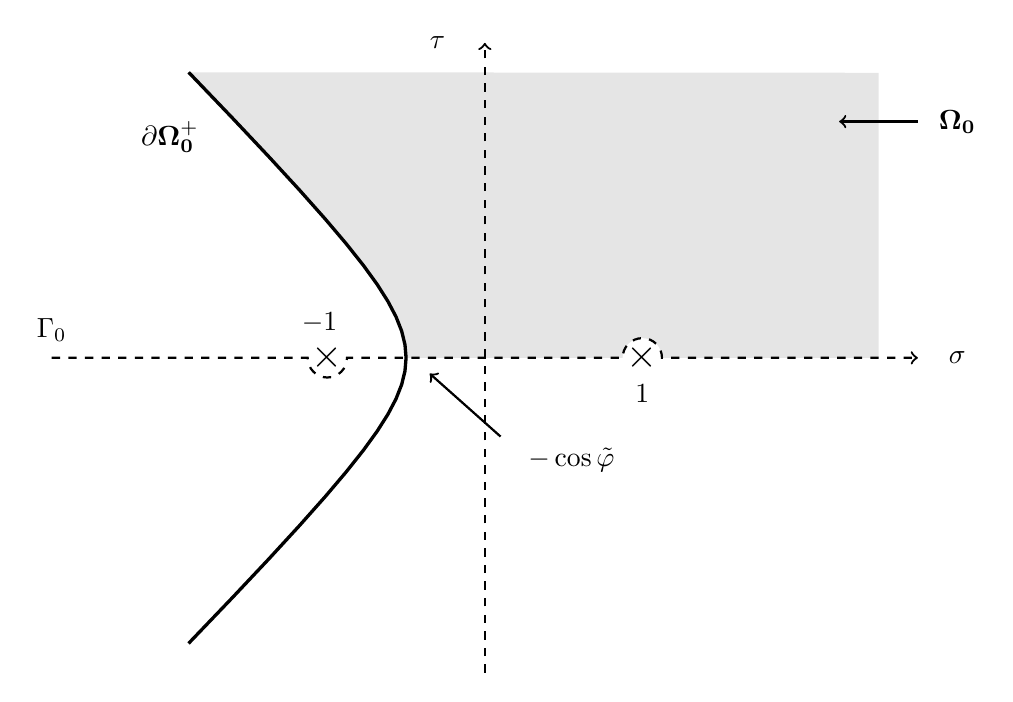
\begin{tikzpicture}
% Filling Omega_0
\fill [color=gray!20]
(5,0)
-- plot [domain=0:2] ({-cosh(\x)},{sinh(\x)})
-- (5,3.62)
-- cycle;

\fill[color=white] (2,0) circle (0.25);

\node at (2,0) {\Large $\mathbf{\times}$}; % Pole
\node at (2,-0.45) { $1$};
\node at (-2,0) {\Large $\mathbf{\times}$};
\node at (-2.1,0.45) {$-1$}; %pole
\node at (-5.5,0.35) {$\Gamma_0$};
\draw[dashed,thick, ->]
      (-5.5,0) -- (-2.25,0)  arc (-180:0:0.25)  -- (1.75,0)arc (180:0:0.25) -- (5.5,0);
\draw[dashed,thick,->]
	  (0,-4) -- (0,4);
\node at (6,0) {$\sigma$};
\node at (-0.6,4) { $\tau$};
      % axis

%% arrows indicating countour deformation
%\draw[ thick, ->] (-3,-0.25) arc (180:235:1);
%\node at (-3.2,-0.9) {$\mathcal{F}_1$};
%\draw[ thick, ->] (4.0,0.3) arc (0:45:1); 
%\node at (4.5,0.8) { $\mathcal{F}_2$};

% Hyperbola (contour  partial_Omega_0 )
\draw[black, very thick][domain=-2:2] plot({-cosh(\x)}, {sinh(\x)});
\node at (-4.0,2.8) { $\mathbf{\partial \Omega_0^+}$};
\draw[thick,->] (0.2,-1.0)--(-0.7,-0.2);
\node at (1.1,-1.3) {$-\cos \phiti$};

%  Omega_0
\draw [thick, ->] (5.5,3)--(4.5,3);
\node at (6,3) {$\mathbf{\Omega_0}$};

\end{tikzpicture}
\caption
[Contour $\partial \Omega_0^+$]
{Domain $\Omega_0$ (the grey area) and its upper boundary $\partial \Omega_0^+$. The lower boundary of $\Omega_0$ is the semi-axis $[-\cos \phiti,+\infty[$.}
\label{chapter5:figure4}
\end{figure}
Having found the system of functional equations, it is now resolved following the methodology of Croisille and Lebeau \cite{CroisilleLebeau}.

\subsection{System resolution}
\label{Chapter5:System_resolution}

The resolution of the system of functional equations \eqref{functional_eq} is necessary in order to find the values of the spectral functions $\hat{\alpha}_1 $ and $\hat{\alpha}_2 $. With these values, the diffraction coefficients can be computed using equation \eqref{GTDCoeff_SF}. 

It is shown in \cite{CroisilleLebeau} that $DM$ and $TM$ integral operators are constituted of a "singular term" and of a "regular term". For a singular function 
\begin{equation}
\label{Chapter5:arbitrary_function}
\phi(\xi) = \dfrac{1}{\xi - z},  \quad z \in \mathbb{C}\setminus ]-\infty,-1] \text{ with } {\rm Im} \, z \geqslant 0,
\end{equation}
$DM$ and $TM$ integral operators defined respectively in \eqref{DM_operator} and \eqref{TM_operator} can be decomposed using the residue theorem as
\begin{subequations}
\label{Int_op_decomp}
\begin{align}
\label{Int_op_decomp_DM}
DM(\phi)(\xi) &= \int_{\Gamma_0} DM(\xi,\lambda) \cdot \dfrac{1}{\lambda - z} \, d \lambda = \dfrac{dm(z)}{\xi - z}  + D_p(\xi,z) \\
\label{Int_op_decomp_TM}
TM(\phi)(\xi) &= \int_{\Gamma_0} TM(\xi,\lambda) \cdot \dfrac{1}{\lambda - z} \, d \lambda = \dfrac{tm(z) }{\xi - T_0(z)} 1_{\Omega_0}(z) + T_p(\xi,z),
\end{align}
\end{subequations}
where the function $T_0$ is defined in \eqref{Trans_operator} and where
\begin{equation}
1_{\Omega_0}(z) = 
\begin{cases}
1 \quad \text{if } z  \in \Omega_0, \\
0 \quad \text{else}
\end{cases}
\end{equation}
and integrals $D_p$ and $T_p$ are holomorphic on $\mathbb{C}\setminus ]-\infty,-1]$. Such integrals are expressed as
\begin{subequations}
\label{holomorphic_functions}
\begin{align}
\label{defDp}
D_p(\xi,z) &= \dfrac{1}{2\pi i}\int_{\Gamma_1} \dfrac{dm(\lambda)}{\xi-\lambda} \cdot \dfrac{1}{\lambda - z} d\lambda, \\
\label{defTp}
T_p(\xi,z) &= \dfrac{1}{2\pi i}\int_{\partial \Omega_0^+}  \dfrac{tm(\lambda)}{\xi-T_0(\lambda)} \cdot \dfrac{1}{\lambda - z} d\lambda.
\end{align}
\end{subequations}
Contours $\Gamma_1$ and $\partial \Omega_0^+$ are illustrated on Figs.~\ref{chapter5:figure5} and \ref{chapter5:figure4} respectively.

\begin{figure}[ht]
\centering
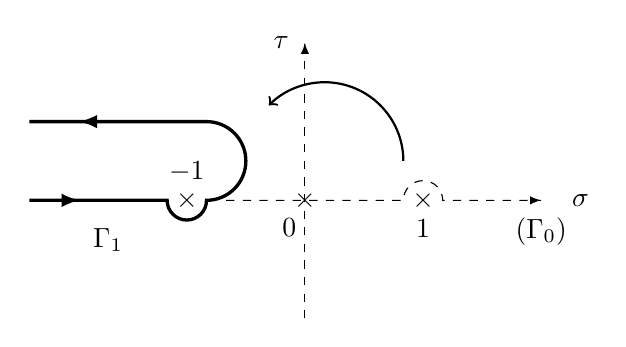
\begin{tikzpicture}
\node at (-0.5,0) {  $\times$};
\node at (-0.7,-0.35) { $0$};
\node at (1,0) { $\times$}; % Pole
\node at (1,-0.36) { $1$};

\node at (-2,0) { $\times$};
\node at (-2,0.36) {  $-1$}; %pole
\node at (-3,-0.5) { $\Gamma_1$};

\draw[dashed, decoration={markings,
 mark=at position 1.0 with {\arrow{latex}}},
      postaction={decorate}] (-1.5,0) -- (0.75,0) arc (180:0:0.25)-- (2.5,0);
\node at (3,0) {$\sigma$};
\draw[dashed, decoration={markings,
 mark=at position 1.0 with {\arrow{latex}}},
      postaction={decorate}] (-0.5,-1.5) -- (-0.5,2);
\node at (-0.8,2) {$\tau$};      

\node at (2.5,-0.4) {$(\Gamma_0)$};
      
\draw[ thick, ->] (0.75,0.5) arc (0:135:1); 
  

\draw[very thick, black, yshift=0pt,
decoration={ markings,  % This schema allows for fine-tuning the positions of arrows 
      mark=at position 0.1 with {\arrow{latex}},
      mark=at position 0.9 with {\arrow{latex}}},
      postaction={decorate}]
      (-4,0) -- (-2.25,0)  arc (-180:0:0.25) -- (-1.75,0) arc(-90:90:0.5)  -- (-4,1);
\end{tikzpicture}
\caption
[Contour $\Gamma_1$]
{Contour $\Gamma_1$. The curved arrow shows the deformation of $\Gamma_0$ (dashed line) into $\Gamma_1$.}
\label{chapter5:figure5}
\end{figure}

In the sequel, using the decomposition of the $DM$ and $TM$ operators for a function of the form of \eqref{Chapter5:arbitrary_function}, it will be shown that the unknown spectral functions $\hat{\alpha}_1$ and $\hat{\alpha}_2$ in the system \eqref{functional_eq} have a singular part. The first step for the resolution of the system \eqref{functional_eq} is then to determine this singular part.

\subsubsection{Singular part}
\label{Chapter5:sing_part}

It is well known that poles of the spectral functions lead to the reflections of the incident field on the wedge faces (these reflections can be multiple), and to the fictitious fields that compensate the incident wave in the shadow zones. The sum of these reflections with the fictitious compensating fields constitute the aforementioned GE field. The singular part of the spectral functions contains these poles. The goal of this subsection is to calculate the poles and the corresponding residues and then to determine the expression of the singular part of the spectral functions, by employing a recursive algorithm. 

Knowing the incident field on the wedge faces, the spectral function  $\hat{\alpha}_j$ can be written as
\begin{equation}
\label{Chapter5:ini_pol_propag}
\hat{\alpha}_j(\xi) = \dfrac{V_j}{\xi - Z_j} + X_j'(\xi), \quad j=1,2
\end{equation}
where $Z_1,Z_2$ are the initial poles, given in (\ref{functional_eq}) with unknown residues $V_1$ and $V_2$ and the functions $X_j'$ are unknown, $j=1,2$. From \eqref{Int_op_decomp_DM}, it is known that
\begin{equation}
\label{Chapter5:pole_propag_DM_1}
DM(\hat{\alpha}_j)(\xi) = \dfrac{dm(Z_j) \cdot V_j}{\xi - Z_j} + D_p(\xi,Z_j)\cdot V_j + DM( X_j')(\xi).
\end{equation}
By choosing $V_j =  dm^{-1}(Z_j).W_j$, the right hand side of the system \eqref{functional_eq} is suppressed by the first term in the right hand side of \eqref{Chapter5:pole_propag_DM_1}. The resulting system's unknown functions are $X'_j, \, j=1,2$ :
\begin{equation}
DM  (X_j' )(\xi)+ TM (X_{3-j}' )(\xi) = - TM  \left(  \dfrac{V_{3-j}}{\xi - Z_{3-j}} \right) (\xi)  - D_p(V_j,Z_j)(\xi) \qquad j=1,2
\end{equation}
Applying \eqref{Int_op_decomp_TM} yields
\begin{equation}
\label{Chapter5:pol_propag_step3}
TM  \left(  \dfrac{V_j}{\xi - Z_j} \right)(\xi) = \dfrac{tm(Z_j) \cdot V_j}{\xi - T_0(Z_j)}  \, 1_{\Omega_0}(Z_j) + T_p(\xi,Z_j)\cdot V_j \qquad j=1,2
\end{equation}
Thus, $X_j'$ has a pole at $\xi = Z_j^{1)} = T_0(Z_{3-j})$ if $Z_{3-j} \in \Omega_0$. The wave incident on face $\mathcal{S}_{3-j}$ is reflected. This reflected wave is incident on face $\mathcal{S}_j$, generating a new pole $Z_j^{(1)}=T_0(Z_{3-j})$. 
The unknown function $X_j'$ in \eqref{Chapter5:ini_pol_propag} is then decomposed as
\begin{equation}
\label{Chapter5:pol_propag_step2}
X_j'(\xi) =  \dfrac{V_j^{(1)}}{\xi - Z_j^{(1)}} + X_j''(\xi), \quad j=1,2
\end{equation}
where the function $ X_j''$ is unknown. 
Once again, the residues $V_j^{(1)}$ of these generated poles $Z_j^{(1)}$ are chosen so that they cancel the singular term in $DM(X_j')(\xi)$, found using formula \eqref{Int_op_decomp_DM}, compensating the singular term in the $TM$ operator in \eqref{Chapter5:pol_propag_step3}.

This pole propagation process is applied recursively in order to determine all the poles of the spectral functions $\hat{\alpha}_j$. This process stops when the generated poles are no longer in the domain $\Omega_0$ defined in \eqref{Domain_Omega0}. All the generated poles then belong to $\Omega_0$. 

At the end of this process, the spectral functions have the following decomposition
\begin{equation}
\label{spec_decomp}
\hat{\alpha}_j=Y_j+X_j, 
\end{equation}
where  $Y_j$ is the singular part, $X_j$ is the regular part  and $j=1,2$ is the face index. The singular part is expressed as
\begin{equation}
\label{sing_part}
 Y_j(\xi) = \sum_i {V_j^{(i)} \over \xi - Z_j^{(i)}},
\end{equation}
where $i \in \mathbb{N}^*$, $Z_j^{(0)} = Z_j$ defined in \eqref{functional_eq} is the initial pole on each face of the wedge, $V_j^{(0)}=V_j$ is the corresponding initial residue on each face of the wedge, 
\begin{equation}
\label{Generated_poles}
Z_j^{(i+1)} = T_0(Z_{3-j}^{(i)}) \quad j=1,2
\end{equation} 
are the different generated poles with their respective residues 
\begin{equation}
\label{Generated_residues}
V_j^{(i+1)}=-dm^{-1}(T_0(Z_{3-j}^{(i)})) \,  tm(Z_{3-j}^{(i)})) \, V_{3-j}^{(i)} \, 1_{\Omega_0}(Z_{3-j}^{(i)}), \quad  j=1,2.
\end{equation}
\paragraph{}
Figure \ref{poles} represents the generated poles in the complex plane for two different cases : figure \ref{poles80} for a wedge of angle $\varphi=80^o$ with an incident angle of $\theta_{inc}=55^o$ and figure \ref{poles20} for $\varphi=20^o$ and $\theta_{inc}=15^o$. As the wedge angle decreases, the number of poles increases, some poles being very close to one another, rendering the method less accurate for very small wedge angles.
\begin{figure}[h]
	\centering
	\begin{subfigure}[b]{0.4\textwidth}
	\begin{tikzpicture}[scale=2]
	\draw[->,>=stealth'] (-1.25,0) -- (1.25,0);
	\draw[->,>=stealth'] (0,-0.5) -- (0,0.5);
	\node at (1.25,0)[right]{Re};
	\node at (0,0.5)[right]{Im};
	
	\node at (-1,0){$\bullet$};
	\node at (1,0){$\bullet$};
	\draw (-1,0) node[below] {$-1$};
	\draw (1,0) node[below] {$1$};
	
	\node at ( 0.573576450    ,  0.00000000    ){$\times$};
	\node at ( 0.906307757    ,  0.00000000    ){$\times$};
	\node at (-0.258819222    ,  0.00000000    ){$\times$};
	\node at (-0.707106829    ,  0.00000000    ){$\times$};
	\end{tikzpicture}
	\subcaption{$\varphi=80^o, \, \theta_{inc}=55^o$}
    \label{poles80}
	\end{subfigure}
\hspace{1em}
\begin{subfigure}[b]{0.4\textwidth}
\begin{tikzpicture}[scale=2]
\draw[->,>=stealth'] (-1.25,0) -- (1.25,0);
\draw[->,>=stealth'] (0,-0.5) -- (0,0.5);
\node at (1.25,0)[right]{Re};
\node at (0,0.5)[right]{Im};

\node at ( 0.965925813    ,  0.00000000    ){$\times$};
\node at ( 0.996194720    ,  0.00000000    ){$\times$};
\node at ( 0.906307876    ,  0.00000000    ){$\times$};
\node at ( 0.819151998    ,  0.00000000    ){$\times$};
\node at ( 0.573576331    ,  0.00000000    ){$\times$};
\node at ( 0.707106948    ,  0.00000000    ){$\times$};
\node at ( 0.422618449    ,  0.00000000    ){$\times$};
\node at ( 0.258818895    ,  0.00000000    ){$\times$};
\node at ( -8.71558934E-02,  0.00000000    ){$\times$};
\node at (  8.71559381E-02,  0.00000000    ){$\times$};

\node at (-1,0){$\bullet$};
\node at (1,0){$\bullet$};
\draw (-1,0) node[below] {$-1$};
\draw (1,0) node[below] {$1$};
\end{tikzpicture}
\subcaption{$\varphi=20^o, \, \theta_{inc}=15^o$}
\label{poles20}
\end{subfigure}
\caption{Poles generated by the recursive algorithm plotted in the complex plane}
\label{poles}
\end{figure}

The second step of the system resolution is the determination of the regular part $X_j$ of the spectral function $\hat{\alpha}_j$, see Eq.~\eqref{spec_decomp}. The regular part is determined by using the Galerkin collocation method. Section \ref{Chapter5:regular_part} gives the principal steps of this resolution method. 

\subsubsection{Regular part}
\label{Chapter5:regular_part}

After the determination of the singular part of the solution using the pole propagation process explained in section \ref{Chapter5:sing_part}, the remaining system \ref{functional_eq} is by construction
\begin{equation}
\label{sys_regular}
\begin{cases}
DM(X_1)(\xi) + TM(X_2)(\xi) = -\underset{k}{\sum} \Big( D_p(\xi,Z_1^{(k)})\cdot V_1^{(k)}+ T_p(\xi,Z_2^{(k)})\cdot V_2^{(k)}\Big)\\
TM(X_1)(\xi) + DM(X_2)(\xi)  =  -\underset{k}{\sum} \Big( T_p(\xi,Z_1^{(k)})\cdot V_1^{(k)}+ D_p(\xi,Z_2^{(k)})\cdot V_2^{(k)}\Big)
\end{cases}
\end{equation}
where $X_j$, $j=1,2$ are the regular parts of the spectral functions \eqref{spec_decomp}, $D_p$ and $T_p$ functions are defined in \eqref{holomorphic_functions} and $Z_j^{(k)}$ are the poles of spectral function $\hat{\alpha}_j$  and their respective residues are $V_j^{(k)}$. According to Croisille and Lebeau \cite{CroisilleLebeau}, $D_p$ and $T_p$ are holomorphic on $\mathbb{C}\setminus  ]-\infty,-1]$ and therefore functions $X_1$ and $X_2$ are also holomorphic on this domain.

The functions $X_j(\xi)$, being holomorphic on $\mathbb{C}\setminus  ]-\infty,-1]$, can be approached in the vectorial subspace generated by $\varphi_k, \, 1 \leq k \leq N$ where
\begin{equation}
\label{Gal_basis}
\varphi_k(\xi) = \dfrac{d_k}{\xi + a_k}, \quad a_k \in [1,\infty[, \quad d_k=\sqrt{\frac{a_k}{\pi}}.
\end{equation}
The approximation of the solution $X_j(\xi)$ in this subspace of finite dimension is called a Galerkin approximation.

In the following, the integration contour $\Gamma_0$ pictured on Fig.~\ref{chapter5:figure2} is deformed into the imaginary axis. If $f(\lambda)$ is a holomorphic function on $\mathbb{C}\setminus  ]-\infty,-1]$, the function $\tilde f (y)=f(iy)$ is introduced so that $\tilde f$ is holomorphic on $\mathbb{C}\setminus i [1,\infty[ $. The variable change $\lambda = iy$ gives a new basis
\begin{equation}
\label{Galerkin_basis}
e_{a_k}(y) = \dfrac{d_k}{y-i{a_k}}=i\tilde \varphi(y), \quad \text{with} \quad d_k=\sqrt{\frac{a_k}{\pi}} \quad \text{and} \quad a_k \in [1,\infty[,
\end{equation}

Having an approximation basis of the regular part of the spectral functions, $X_j(\xi)$ can be expressed as
\begin{equation}
\label{regular_part_decomp}
X_j(\xi) \approx \sum_{k=1}^N \tilde{X}_j^k \, \varphi_k(\xi), \quad \tilde{X}_j^k \in \mathbb{C}.
\end{equation}
The coordinates $\tilde{X}_j^k$ are unknown. The system \eqref{sys_regular} then becomes, for $j=1,2$
\begin{equation}
\label{sys_regular_gal}
\sum_{k=1}^N \left[ \tilde{X}_j^k \, \int_{\Gamma_0} DM(\xi,\lambda) \varphi_k(\lambda) \, {\rm d} \lambda + \tilde{X}_{3-j}^k \, \int_{\Gamma_0} TM(\xi,\lambda) \varphi_k(\lambda) \, {\rm d} \lambda \right] = u_j(\xi), 
\end{equation}
where
\begin{equation}
\label{second_member}
u_j(\xi) = -\sum_k \Big( D_p(\xi,Z_j^k)\cdot V_j^k+ T_p(\xi,Z_{3-j}^k)\cdot V_{3-j}^k\Big) \qquad j=1,2
\end{equation}
The variable changes $\lambda = iy$ and $\xi = ix$ in \eqref{sys_regular_gal} lead to the following system $(j=1,2)$
\begin{equation}
\label{sys_regular_gal_def}
\sum_{k=1}^N \left[ \tilde{X}_j^k \, \int_{-\infty}^\infty  \widetilde{DM}(x,iy) \, e_{a_k}(y) {\rm d} y + \tilde{X}_{3-j}^k \, \int_{-\infty}^\infty  \widetilde{TM}(x,iy) \, e_{a_k}(y) {\rm d} y \right] = \tilde u_j(x) \\
\end{equation}
where $\widetilde{DM}(x,iy) = DM(ix,iy)$ and $\widetilde{TM}(x,iy) = TM(ix,iy)$. Following \cite{CroisilleLebeau}, we introduce another subspace of finite dimension in $L^2(\mathbb{R})$ which is generated by vectors $e_{b_k}$ with
\begin{equation}
\label{points_collocation}
e_{b_k}(y)=\frac{d_k}{y-ib_k}, \quad  \rm Re (b_k) \in [1,\infty[  \quad \text{and}  \quad {\rm Im} (b_k) = 0^-.
\end{equation}

Points $b_k$ are called collocation points.  The system \eqref{sys_regular_gal_def} is projected in this subspace using the following relation :
\begin{equation}
\label{dot_product}
\langle \tilde \phi\vert e_{b_k}\rangle_{L^2(\mathbb R)}= (-2i\pi) \, d_k \,  \phi (b_k)
\end{equation}

Using \eqref{dot_product}, the projection of the system \eqref{sys_regular_gal_def} leads to the following new system (for $j=1,2$)
\begin{equation}
\label{sys_regular_gal_col}
\begin{cases}
\sum_{k=1}^N \left[ \tilde{X}_j^k \, \int_{-\infty}^\infty DM(b_1,iy) e_{a_k}(y) \, {\rm d} y + \tilde{X}_{3-j}^k \, \int_{-\infty}^\infty TM(b_1,iy) e_{a_k}(y) \, {\rm d} y \right] = u_j(b_1) \\
 \qquad \qquad \qquad \qquad \qquad \qquad \qquad \qquad \vdots \\
\sum_{k=1}^N \left[ \tilde{X}_j^k \, \int_{-\infty}^\infty DM(b_N,iy) e_{a_k}(y) \, {\rm d} y + \tilde{X}_{3-j}^k \, \int_{-\infty}^\infty TM(b_N,iy) e_{a_k}(y) \, {\rm d} y \right] = u_j(b_N)
\end{cases}
\end{equation}
The obtained system \eqref{sys_regular_gal_col} is a linear system of equations and can be put in a matrix format:
\begin{equation}
\label{Syst_lineaire}
\begin{pmatrix}
\mathbb{D} & \mathbb{T}\\
\mathbb{T} & \mathbb{D}
\end{pmatrix}
\;
\begin{pmatrix}
\mathbb{X}_1\\
\mathbb{X}_2
\end{pmatrix}
 = 
\begin{pmatrix}
\mathbb{U}_1\\
\mathbb{U}_2
\end{pmatrix}
\end{equation}
where
\begin{equation}
\mathbb{X}_j = 
\begin{pmatrix}
\tilde{X}_j^1 \\
\vdots \\
\tilde{X}_j^N
\end{pmatrix}
\, \tilde{X}_j^k \in \mathbb{C}; \quad
\mathbb{U}_j = 
\begin{pmatrix}
u_j(b_1)\\
\vdots\\
u_j(b_N)\\
\end{pmatrix}
\, u_j(b_k) \in \mathbb{C}
\end{equation} 
and 
\begin{equation}
\label{D_matrix}
\mathbb{D}_{lk} = \int_{-\infty}^\infty DM(b_l,iy) e_{a_k}(y) \, {\rm d} y
\end{equation}
\begin{equation}
\label{T_matrix}
\mathbb{T}_{lk} = \int_{-\infty}^\infty TM(b_l,iy) e_{a_k}(y) \, {\rm d} y
\end{equation}
are the matrix elements of $\mathbb{D}$ and $\mathbb{T}$ respectively. System \eqref{Syst_lineaire} can be rewritten as
\begin{equation}
\label{Syst_lineaire_mod}
\begin{cases}
(\mathbb{D} + \mathbb{T}) \, (\mathbb{X}_1 + \mathbb{X}_2) = \mathbb{U}_1 +  \mathbb{U}_2\\
(\mathbb{D} - \mathbb{T}) \, (\mathbb{X}_1 - \mathbb{X}_2) = \mathbb{U}_1 - \mathbb{U}_2
\end{cases}.
\end{equation}
To approximate the regular part of the spectral functions \eqref{regular_part_decomp}, its coordinates $\tilde{X}_j^k$ in the Galerkin basis $\varphi_k, \, 1 \leq k \leq N$ defined in \eqref{Gal_basis} must be determined. These coordinates are the solutions of the linear system of equations \eqref{Syst_lineaire} or \eqref{Syst_lineaire_mod}. To resolve such a system, the matrices $\mathbb{D}$ and $\mathbb{T}$ and the right hand side $\mathbb{U}_{1,2}$ must be computed. 

\paragraph{Matrix calculation}

The first step is to determine $\mathbb{D}$ and $\mathbb{T}$ matrices.
Using \eqref{DM_operator} and \eqref{Galerkin_basis}, the $\mathbb{D}_{lk}$ elements defined in \eqref{D_matrix} can be expressed as
\begin{equation}
\label{matrice_D}
(-2i\pi) \mathbb{D}_{lk} =  -i d_k \mathcal{D}(a_k,b_l)
\end{equation}
with the function $\mathcal{D}(a,b)$ defined for $a>1$ and $b>1$ as
\begin{equation}
\label{ldbis}
\mathcal{D}(a,b) = \int_{-\infty}^{+\infty} \dfrac{dm(iy)}{y + ib} \, \dfrac{1}{y -ia} dy 
% = \int_{-\infty}^{+\infty} \dfrac{1}{y + ib} \, \dfrac{1}{y -ia} \, \dfrac{1}{\zeta_0^0(iy)} {\rm d}y. 
\end{equation}
This integral's value can be determined analytically. The details of the computation being a bit heavy, they are given in appendix \ref{finalDac}.

Using \eqref{TM_operator} and \eqref{Galerkin_basis} the $\mathbb{T}_{lk}$ elements defined in \eqref{T_matrix} can be expressed as
\begin{equation}
\label{matrice_T}
(-2i\pi) \mathbb{T}_{lk} =  - d_k \mathcal{T}(a_k,b_l)
\end{equation}
where the function $\mathcal{T}(a,b)$ is defined for $a>1$ and $b>1$ as
\begin{equation}
\label{ltbis}
\mathcal{T}(a,b) = \int_{-\infty}^{+\infty} \dfrac{tm(iy)}{ b - iy \cos 2\varphi  + |\sin 2\varphi| \sqrt{1+y^2}} \, \dfrac{1}{y -i a} \, dy . 
\end{equation}
This integral's value can be determined analytically. The details of the computation being a bit heavy, they are given in appendix \ref{finalTac}.

The matrices $\mathbb{D}$ and $\mathbb{T}$ are completely determined using \eqref{matrice_D} and \eqref{matrice_T} respectively. Their analytical properties are also known. In order to resolve the linear system of equations \eqref{Syst_lineaire} or \eqref{Syst_lineaire_mod},  their right hand side constituted of $\mathbb{U}_1$ and $\mathbb{U}_2$ must also be computed.

\paragraph{Determination of the right hand side of the system of equations}

Using \eqref{second_member}, the right hand side of the system \eqref{sys_regular_gal_col} which is calculated at the collocation points $b_l$ defined in \eqref{points_collocation}, $l \in \{ 1,2, \ldots, N \}$, is 
\begin{equation}
\label{second_member_new}
u_j(b_l) = -\sum_k \Big( D_p(b_l,Z_j^k)\cdot V_j^k+ T_p(b_l,Z_{3-j}^k)\cdot V_{3-j}^k\Big) \qquad j=1,2
\end{equation}
where $D_p$ and $T_p$ functions are defined in \eqref{Int_op_decomp} and $Z_j^k$ is defined in \eqref{Generated_poles}, $k \in \mathbb{N}^*$. 

Taking the definition of the $D_p$ function in \eqref{Int_op_decomp_DM}, and deforming the contour $\Gamma_0$ pictured on Fig.~\ref{chapter5:figure2} into the imaginary axis by applying the variable change $\lambda = iy$, we get
\begin{equation}
\label{Dp_final}
D_p(b_l,z) = {1\over 2\pi}\mathcal D(-z,b_l)-  {m(z)\over b_l-z}.
\end{equation}

Similarly, using the definition of the $T_p$ function given in \eqref{Int_op_decomp_TM}, and by deforming the integrand contour $\Gamma_0$ pictured on Fig.~\ref{chapter5:figure2} into the imaginary axis by applying the variable change $\lambda = iy$ we have
\begin{equation}
\label{Tp_final}
T_p(b_l,z) = 
\dfrac{1}{2i\pi} \mathcal T(-z,b_l) - \dfrac{m(z)}{b_l - T_0(z)} \mathbf{1} (z \in \Omega_0) .
\end{equation}

Expressions \eqref{Dp_final} of $D_p$ and \eqref{Tp_final} of $T_p$ functions are incorporated in the right hand side of the system \eqref{second_member_new} with $z = Z_j^k$ for each $u_j(b_l), \, j=1,2$. In this new expression, with the pole propagation process explained in section \ref{Chapter5:sing_part}, singular terms of $D_p$ and $T_p$ functions cancel each other. The remaining term in the right hand side of the system \eqref{second_member_new} is therefore, for $j=1,2; \quad l \in \{ 1,2, \ldots, N \}$
\begin{equation}
(2\pi i) \, u_j(b_l) =  - \sum_k \left( i \mathcal D(-Z_j^k,b_l)\cdot V_j^k  + \mathcal T(-Z_{3-j}^k,b_l) 
\cdot V_{3-j}^k  \right) +  \dfrac{2\pi i}{b_l - Z_j}
\end{equation}

Once all matrix terms have been calculated, system \eqref{Syst_lineaire} is resolved numerically using the numeric library Eigen for C++. With the resolution of this linear system of equations, the coordinates $\tilde{X}_j^k$ of the regular term $X_j$ of the spectral functions are known and therefore the regular term $X_j$ is approximated using \eqref{regular_part_decomp}. The spectral functions $\hat{\alpha}_j$ are then completely determined using \eqref{spec_decomp}, \eqref{sing_part} and \eqref{regular_part_decomp}. 

\subsection{Propagation of the solution}
\label{propag_sol}
The regular part approximation described previously is not accurate in the entire complex plane. There exists a procedure, called "propagation of the solution", which allows to propagate the accuracy of the regular part $X_j(\xi)$ of the spectral functions from $\xi \notin \Omega_0^-$, ${\rm Im} (\xi) <0$ where the approximation is valid to the domain $\Omega_0^-$ where it is not. The space $\Omega_0^-$ defined by
\begin{equation}
\label{defomegamoins}
\Omega_0^- = \{\xi \in \mathbb C, \ {\rm Im}(\xi) <0, \  \xi=\cos(\theta), \ \phiti < {\rm Re}(\theta)<\pi\}
\end{equation}
is represented in Fig.~\ref{chapter5:figure11}. 
The procedure consists in deriving new recursive equations by deforming the  contour $\Gamma_0$ in the integrals of the right-hand side of \eqref{sys_regular} into a new contour $\Gamma_2$ and taking into account the poles crossed in the process.

To begin, the contour $\Gamma_0$ in the $DM$ integral operator is deformed into $\Gamma_2$. The half-space $\{ \lambda, {\rm Im} \ \lambda < 0 \}$ is then crossed during this contour deformation as shown by the $F_1$ arrow on Fig.~\ref{chapter5:figure8}.

\begin{figure}[ht]%
\centering
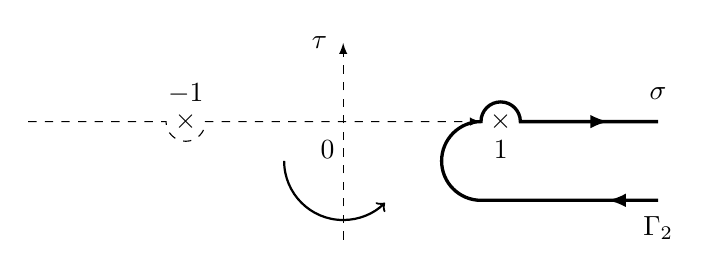
\begin{tikzpicture}
%\node at (-0.5,0) {  $\times$};
\node at (-0.2,-0.35) { $0$};
\node at (2,0) { $\times$}; % Pole
\node at (2,-0.36) { $1$};

\node at (-2,0) { $\times$};
\node at (-2,0.36) {  $-1$}; %pole
\node at (4,-1.35) { $\Gamma_2$};

\draw[dashed, decoration={markings,
 mark=at position 1.0 with {\arrow{latex}}},
      postaction={decorate}] (-4,0) -- (-2.25,0) arc (-180:0:0.25)-- (1.75,0);
      
\node at (4,0.35) {$\sigma$};

\draw[dashed, decoration={markings,
 mark=at position 1.0 with {\arrow{latex}}},
      postaction={decorate}] (0,-1.5) -- (0,1);
\node at (-0.3,1) {$\tau$};      

%\node at (2.5,-0.4) {$(\Gamma_0)$};
      
\draw[ thick, ->] (-0.75,-0.5) arc (0:135:-0.75); 
  

\draw[very thick, black, yshift=0pt,
decoration={ markings,  
      mark=at position 0.1 with {\arrow{latex}},
      mark=at position 0.9 with {\arrow{latex}}},
      postaction={decorate}]
      (4,-1) -- (1.75,-1)  arc (90:-90:-0.5) -- (1.75,0) arc(180:0:0.25)  -- (4,0);
\end{tikzpicture}
\caption
[Contour $\Gamma_2$]
{Contour $\Gamma_2$. The curved arrow shows the deformation of $\Gamma_0$ (dashed line) into $\Gamma_2$.}
\label{chapter5:figure8}
\end{figure}

During this contour deformation, only the poles
\begin{equation}
\lambda = \xi, \quad \text{with } {\rm Im}(\xi) <0 
\end{equation}
of the $DM$ function \eqref{DM_operator} are crossed and therefore, applying the residue theorem, we have for $\xi \in \mathbb{C}$, ${\rm Im}(\xi) <0$, $j=1,2$, 
\begin{equation}
\label{DM_propag_sol}
DM(X_j)(\xi) = \int_{\Gamma_0} DM(\xi,\lambda) X_j(\lambda) \, {\rm d} \lambda  = \int_{\Gamma_2} DM(\xi,\lambda) X_j(\lambda) \, {\rm d} \lambda + m(\xi) X_j(\xi).
\end{equation}

The poles of the $TM$ function \eqref{TM_operator} are
$$ \lambda = T_0^{-1}(\xi) = \xi \, \cos \widetilde{2\varphi}  - \sin \widetilde{2\varphi} \, \zeta_0(\xi) = \cos (\theta - \widetilde{2\varphi}) \quad \text{if} \quad \xi = \cos \theta $$
$T_0^{-1}$ operates in the domain $\Omega_0^-$, therefore they are crossed during this contour deformation if and only if $\xi \in \Omega_0^-$ (see dotted area on Fig.~\ref{chapter5:figure11}).
The domain $\Omega_0^-$ is delineated by the hyperbola 
\begin{equation}
\partial \Omega_0^- = \{   \xi \in \mathbb{C}, \ {\rm Im}(\xi) <0,  \xi = \cos \theta, {\rm Re} \, \theta = \widetilde{2\varphi} \}.
\end{equation}
Domain $\Omega_0^-$ and contour $\partial \Omega_0^-$ are illustrated on Fig.~\ref{chapter5:figure11}.   

Applying the residue theorem to the $TM$ integral operator then gives for $\xi \in \mathbb{C}$, ${\rm Im}(\xi) <0$, $j=1,2$,
\begin{equation}
\label{TM_propag_sol}
TM(X_j)(\xi) = \int_{\Gamma_0} TM(\xi,\lambda) X_j(\lambda) \, {\rm d} \lambda  = \int_{\Gamma_2} TM(\xi,\lambda) X_j(\lambda) \, {\rm d} \lambda + m(\xi) \, X_j[T_0^{-1}(\xi)] \mathbf{1}(\xi \in \Omega_0^-)
\end{equation}

\begin{figure}[ht]%
\begin{center}
	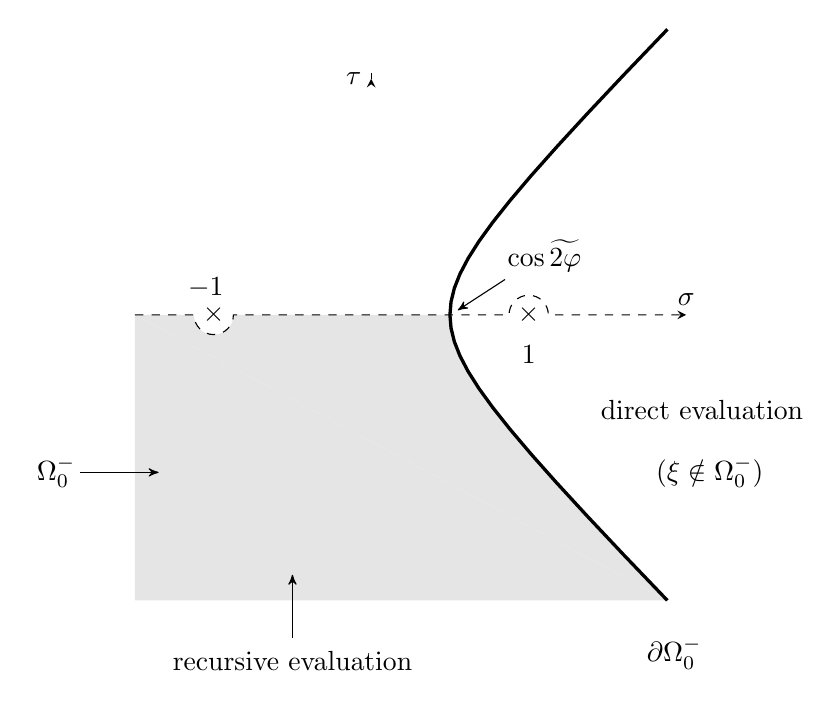
\begin{tikzpicture}
		% Filling Omega_0^-
	\fill [color=gray!20]
	(-1,0)
	-- plot [domain= 0:2] ({cosh(\x)},{-sinh(\x)})
	-- (-3,0)
	-- cycle;
	
	\fill [color=gray!20]
	({cosh(2)},{-sinh(2)})
	-- plot [domain= 0:-3] ({\x},{-sinh(2)})
	-- (-3,0)
	-- cycle;
	
	\fill[color=white] (-2,0) circle (0.25);
	
	\draw[dashed, ->,>=stealth] (-3,0)  -- (-2.25,0) arc(-180:0:0.25)--(1.75,0) arc (180:0:0.25)--(4,0) node[above]{$\sigma$};
	\draw[dashed, ->,>=stealth](0,3)--(0,3) node[left]{$\tau$};
	
	\node at (2,0) {$\times$}; % Pole
	\node at (2,-0.5) {$1$};
	\node at (-2,0) { $\times$};
	\node at (-2.1,0.35) {$-1$}; %pole
	
	% Hyperbola (contour  partial_Omega_0 )
	\draw[black, very thick][domain=-2:2] plot({cosh(\x)}, {-sinh(\x)});
	\node at (3.85,-4.3) {$\partial \Omega_0^-$};
	\draw[thin, ->,>=stealth'](1.7,0.45) -- (1.1, 0.06);
	\node at (2.2, 0.75) {$\cos \widetilde{2\varphi}$};
	
	% Omega_0
	\node at (-4,-2) {$\Omega_0^-$};
	\draw[->,>=stealth'] (-3.7, -2) -- (-2.7,-2);
	\draw[->,>=stealth'] (-1,-4.1) -- (-1,-3.3);
	\node at (-1,-4.4) {recursive evaluation};
	\node at (4.2,-1.2) { direct evaluation};
    \node at (4.3,-2) { $(\xi \notin \Omega_0^-)$};
	
	\end{tikzpicture}
\end{center}
\caption
[Domain $\Omega_0^-$ and its lower boundary $\partial \Omega_0^-$]
{Domain $\Omega_0^-$ and its lower boundary $\partial \Omega_0^-$ in the complex plane $\xi=\sigma + i \tau$. $\Omega_0^-$ is delimited by $\partial \Omega_0^-$ andthe semi-axis $]-\infty, \cos \widetilde{2\varphi}]$. }
\label{chapter5:figure11}
\end{figure}


Using \eqref{DM_propag_sol} and \eqref{TM_propag_sol} in the system of functional equations \eqref{sys_regular}, the system \eqref{sys_regular} is then equivalent to this new system for $\xi \in \mathbb{C}$, ${\rm Im}(\xi) <0$:
\begin{equation}
\label{propag_sol_sys}
\begin{cases}
X_1(\xi) = g_1(\xi) -  X_2(T_0^{-1}(\xi)) \, \mathbf{1}(\xi \in \Omega_0^-) \\
\\
X_2(\xi) = g_2(\xi) - X_1(T_0^{-1}(\xi)) \, \mathbf{1}(\xi \in \Omega_0^-) 
\end{cases}
\end{equation}
where
\begin{equation}
g_j(\xi) = m(\xi)^{-1} \left[ u_j(\xi) - \int_{\Gamma_2} DM(\xi,\lambda) \, X_j(\lambda) \, {\rm d} \lambda - \int_{\Gamma_2} TM(\xi,\lambda) \, X_{3-j}(\lambda) \, {\rm d} \lambda \right] \\
\end{equation}
Formula \eqref{propag_sol_sys} is called the recursive formula because it uses the value of the regular function $X_2$ at point $T_0^{-1}(\xi)$ to compute the value of $X_1$ at the point $\xi$ where the approximation is not valid (and vice-versa). If the translation from $\xi$ to $T_0^{-1}(\xi)$ is not sufficient to reach the domain $\mathbb{C} \backslash \Omega_0^-$ where the approximation is valid, then the use of the formula is repeated as many times as necessary (computing $X_2(T_0^{-1}(\xi))$ using the value of $X_1(T_0^{-2}(\xi))$, etc.).

To calculate $g_j$ functions, we need to compute
\begin{equation*}
\int_{\Gamma_2} DM(\xi,\lambda) \, X_j(\lambda) {\rm d} \lambda =\sum_k \tilde{X}_j^k \int_{\Gamma_2} DM(\xi,\lambda) \, \varphi_k(\lambda) \, {\rm d} \lambda 
\end{equation*}
and
\begin{equation*}
\int_{\Gamma_2} TM(\xi,\lambda) \, X_j(\lambda) {\rm d} \lambda = \sum_k \tilde{X}_j^k \int_{\Gamma_2} TM(\xi,\lambda) \, \varphi_k(\lambda) \, {\rm d} \lambda
\end{equation*}

If ${\rm Im}(a) < 0$, the residue theorem combined with the variable change $\lambda = iy$  yields
\begin{equation}
\int_{\Gamma_2} DM(\xi,\lambda) \,  \dfrac{1}{\lambda+a} \, \, {\rm d} \lambda =  \dfrac{1}{2\pi} \, \mathcal{D}(a,\xi) - \dfrac{m(\xi)}{\xi +a} = \mathcal{ND}(a,\xi). 
\end{equation}

For the $TM$ contributions, the poles $\lambda = T_0^{-1}(\xi)$ are taken into account if and only if $\xi \in \Omega_0^-$. Thus, for $\xi \in \Omega_0^-$, ${\rm Im}(a) < 0$, the residue theorem combined with the variable change $\lambda = iy$ gives
\begin{equation}
\int_{\Gamma_2} TM(\xi,\lambda) \,  \dfrac{1}{\lambda +a} \, \, {\rm d} \lambda = \frac{1}{2i\pi} \mathcal{T}(a,\xi)- \dfrac{m(\xi)}{T_0^-(\xi) +a}   =  \mathcal{NT}(a,\xi)
\end{equation}

Formula \eqref{regular_part_decomp} finally leads to, for $\xi \in \Omega_0^-$ and $j=1,2$,
\begin{eqnarray}
m(\xi)\, g_j(\xi) -  u_j(\xi)=
-\Big( \sum_k \tilde X_j^{k}\, d_k \, N\mathcal D(a_k,\xi)+\sum_k \tilde X_{3-j}^{k} \, d_k \,
N\mathcal T(a_k,\xi) \Big) \nonumber
\end{eqnarray}

Some numerical results are presented in the sequel.

\section{Numerical results}
\label{Chapter5:results}

In this section, a far-field ($k_0r>>1$) asymptotic evaluation of the diffraction coefficient is computed using the stationary phase method :
\begin{equation}
\label{GTDCoeff_SF}
D(\theta) = \dfrac{e^{-i\frac{\pi}{4}}}{\sqrt{2\pi}} \, [\hat{\alpha}_1( - \cos \theta) + \hat{\alpha}_2( - \cos ( 2\varphi - \theta))]
\end{equation}
where $\hat{\alpha}_1$ and $\hat{\alpha}_2$ are the spectral functions, is compared to the analytic expression of the diffraction coefficient of the scattering of a plane wave with a wedge at interfaces fluid/void as expressed by Sommerfeld \cite{Sommerfeld}. Keller \cite{GTD} gives an analytical expression of the GTD approximation of the coefficient in the case of the diffraction of a scalar plane wave by a wedge with Dirichlet boundaries which can be used in the case of a stress-free wedge immersed in a fluid :
\begin{align}
\label{GTDCoeff_Dir}
D^{\rm (Dir)}(\theta) = \dfrac{e^{i\frac{\pi}{4}}}{2N \sqrt{2\pi}}  \, \left[ \cot \left( \dfrac{\pi + (\theta + \theta_{\rm inc})}{2N} \right) + \cot \left( \dfrac{\pi - (\theta + \theta_{\rm inc})}{2N} \right) \right.   \nonumber \\
\left. - \cot \left( \dfrac{\pi + (\theta - \theta_{\rm inc})}{2N} \right) - \cot \left( \dfrac{\pi - (\theta - \theta_{\rm inc})}{2N} \right) \right],
\end{align}
with $N=2\varphi/\pi$.

To apply the recursive procedure described in \ref{propag_sol}, calculation points $\xi$ must have a negative imaginary part. The calculation points considered are then
\begin{equation}
\label{calculation_points_recursive}
\xi_1 = -\cos \theta -i\,10^{-3}  \quad \text{and} \quad \xi_2=- \cos (2\varphi - \theta) - i\, 10^{-3} ,
\end{equation}
where $\theta$ is the observation angle in the wedge (see Fig.~\ref{chapter5:figure1}).

For the Galerkin basis defined in \eqref{Galerkin_basis}, the parameters $a_k \in [1,\infty[$ are chosen as an exponential law \cite{CroisilleLebeau}:
\begin{equation}
\begin{split}
\label{bas_Gal}
a_k &= 1.1 + 0.05 \left( 10^{\frac{k -1}{4}} - 1 \right), \quad 1\leq k\leq 20 \\
b_k &= a_k  - i 0.1, \quad 1\leq k\leq 20 .
\end{split}
\end{equation}

The module of the diffraction coefficients computed using spectral functions and Sommerfeld integral method for various wedge angles are plotted in terms of the observation angle $\theta, \quad 0\leq \theta\leq 2\varphi$ and presented on Fig.~\ref{chapter5:figure12}. 
\begin{figure}[h!]
\centering
\begin{subfigure}[b]{0.49\textwidth}
        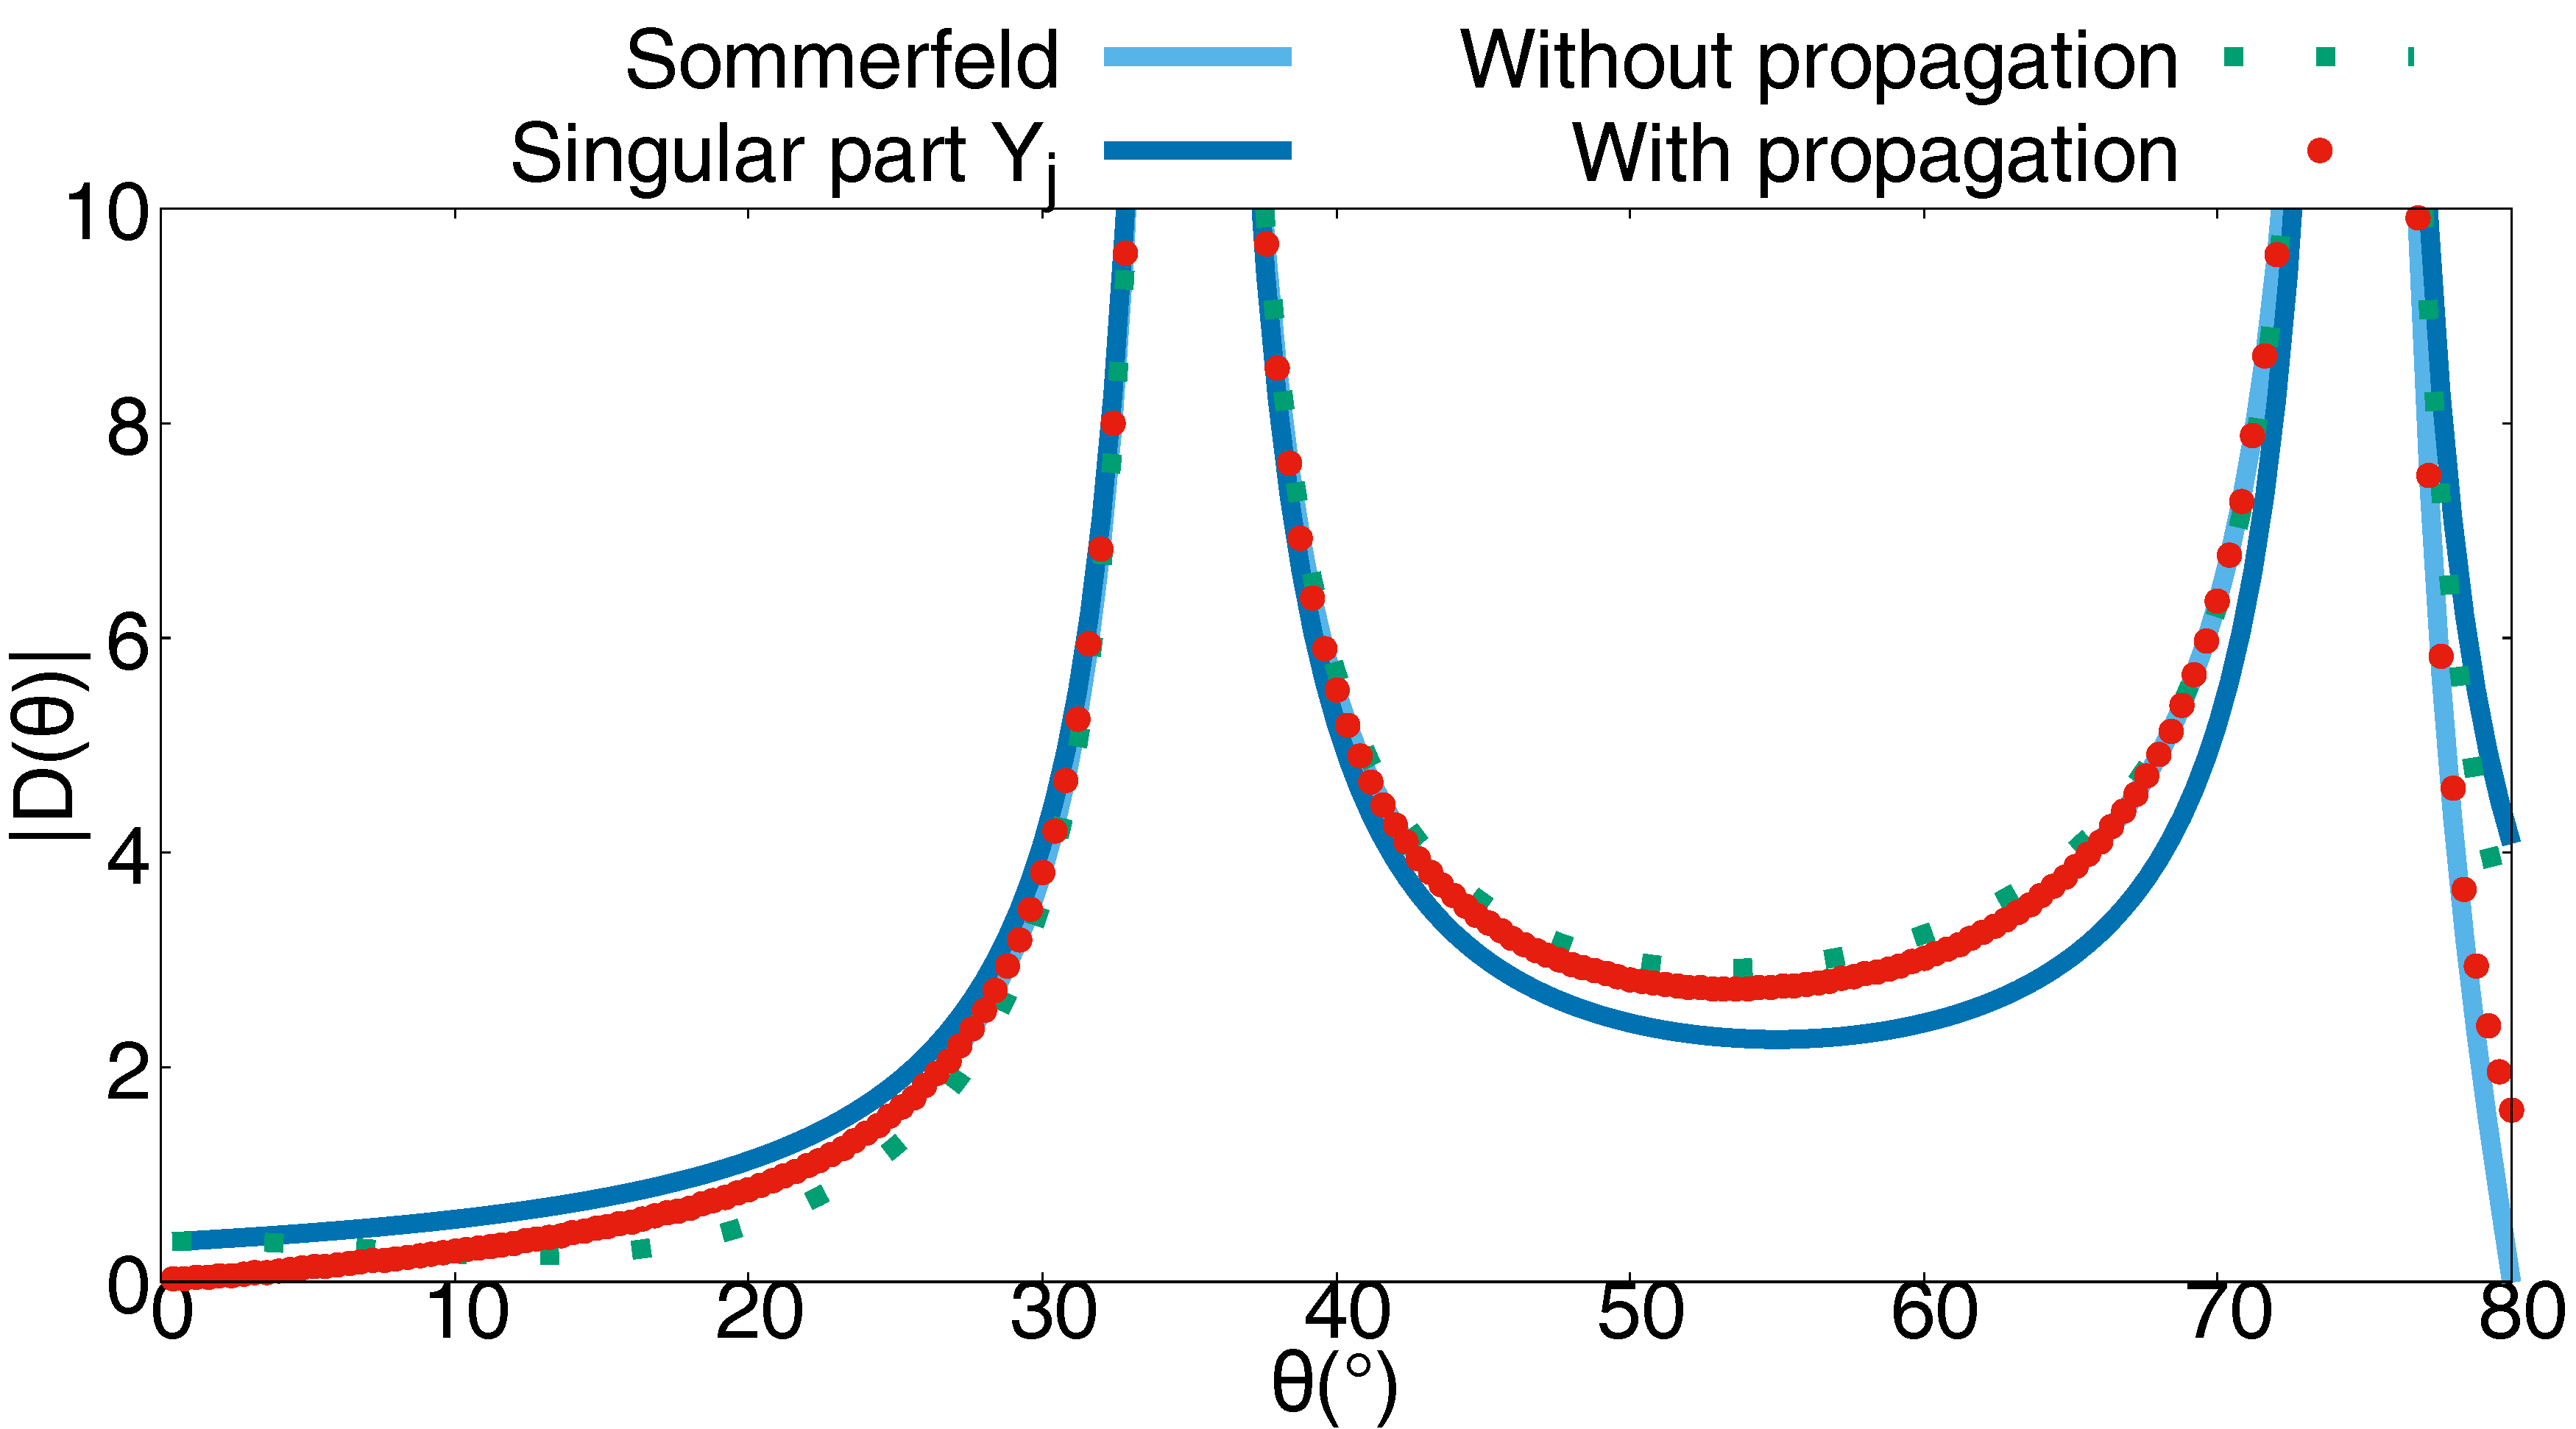
\includegraphics[width=\textwidth]{images/chapter2/Figure8a.pdf}
        \caption{$2\varphi = 80^o$, $\theta_{\rm inc} = 55^o$}
        \label{chapter5:figure12a}
    \end{subfigure}
\begin{subfigure}[b]{0.49\textwidth}
        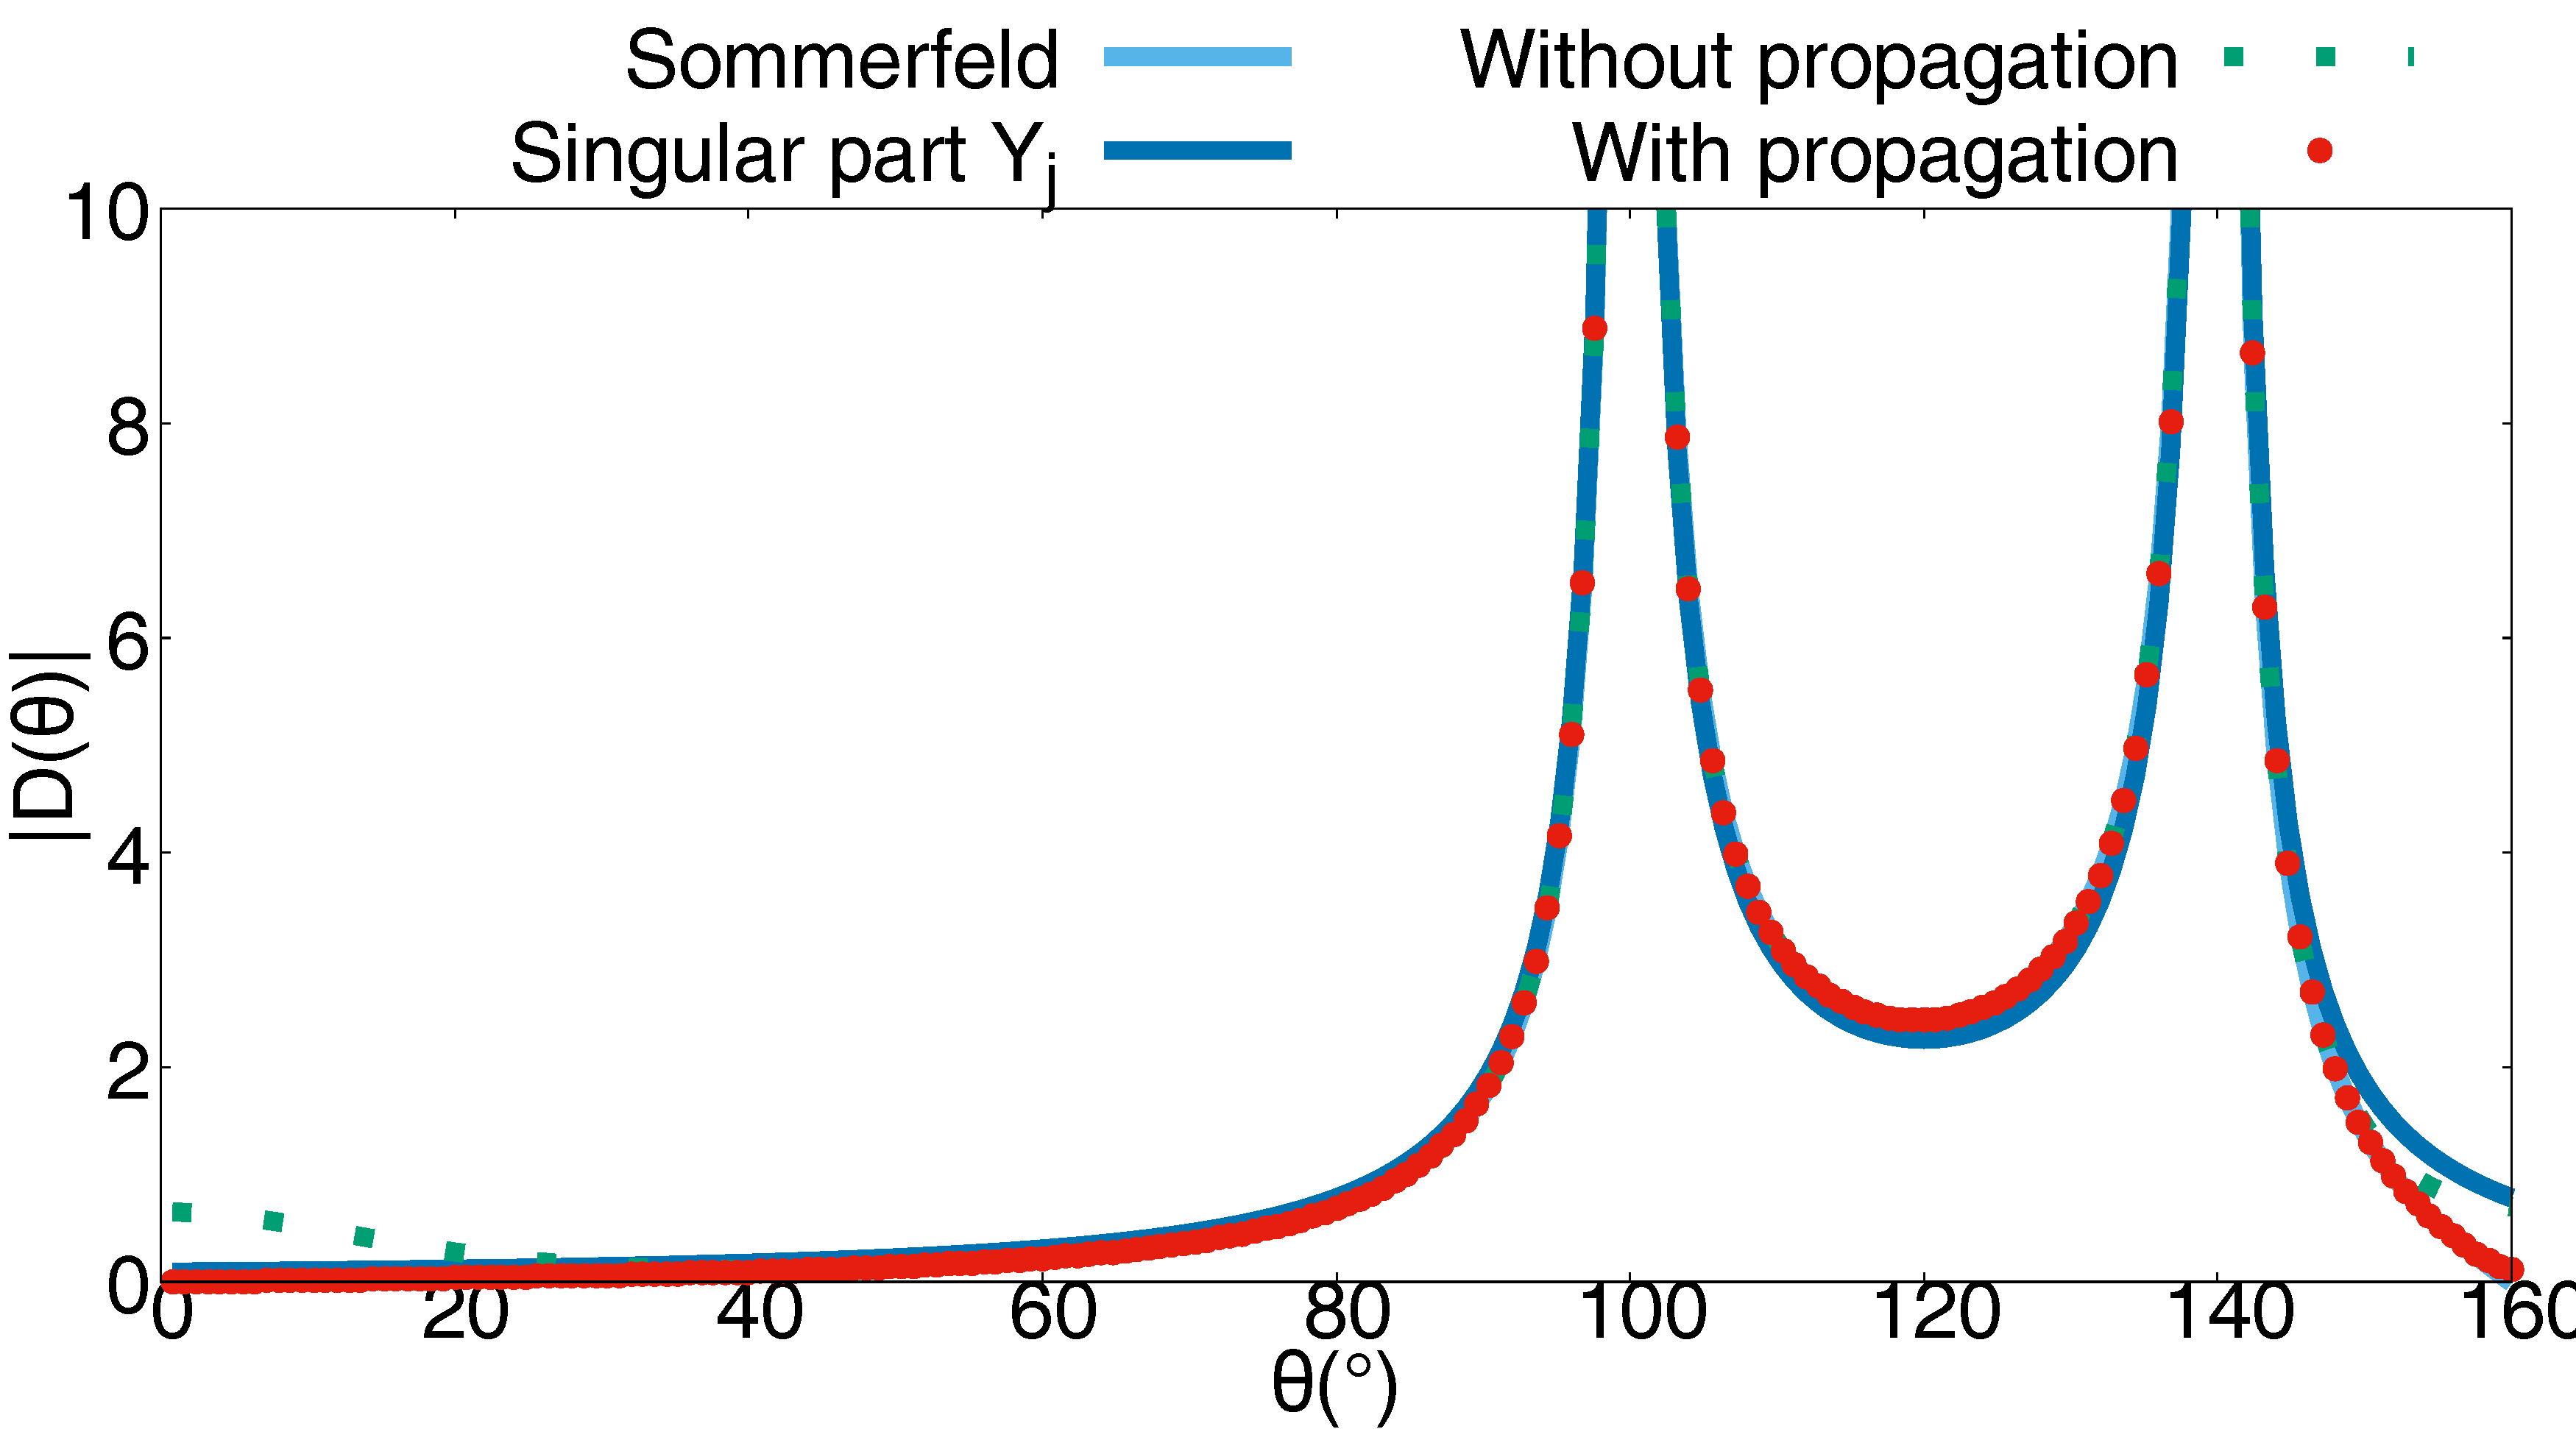
\includegraphics[width=\textwidth]{images/chapter2/Figure8b.pdf}
        \caption{$2\varphi = 160^o$, $\theta_{\rm inc} = 40^o$}
        \label{chapter5:figure12b}
    \end{subfigure}
\\
~\\
\begin{subfigure}[b]{0.49\textwidth}
        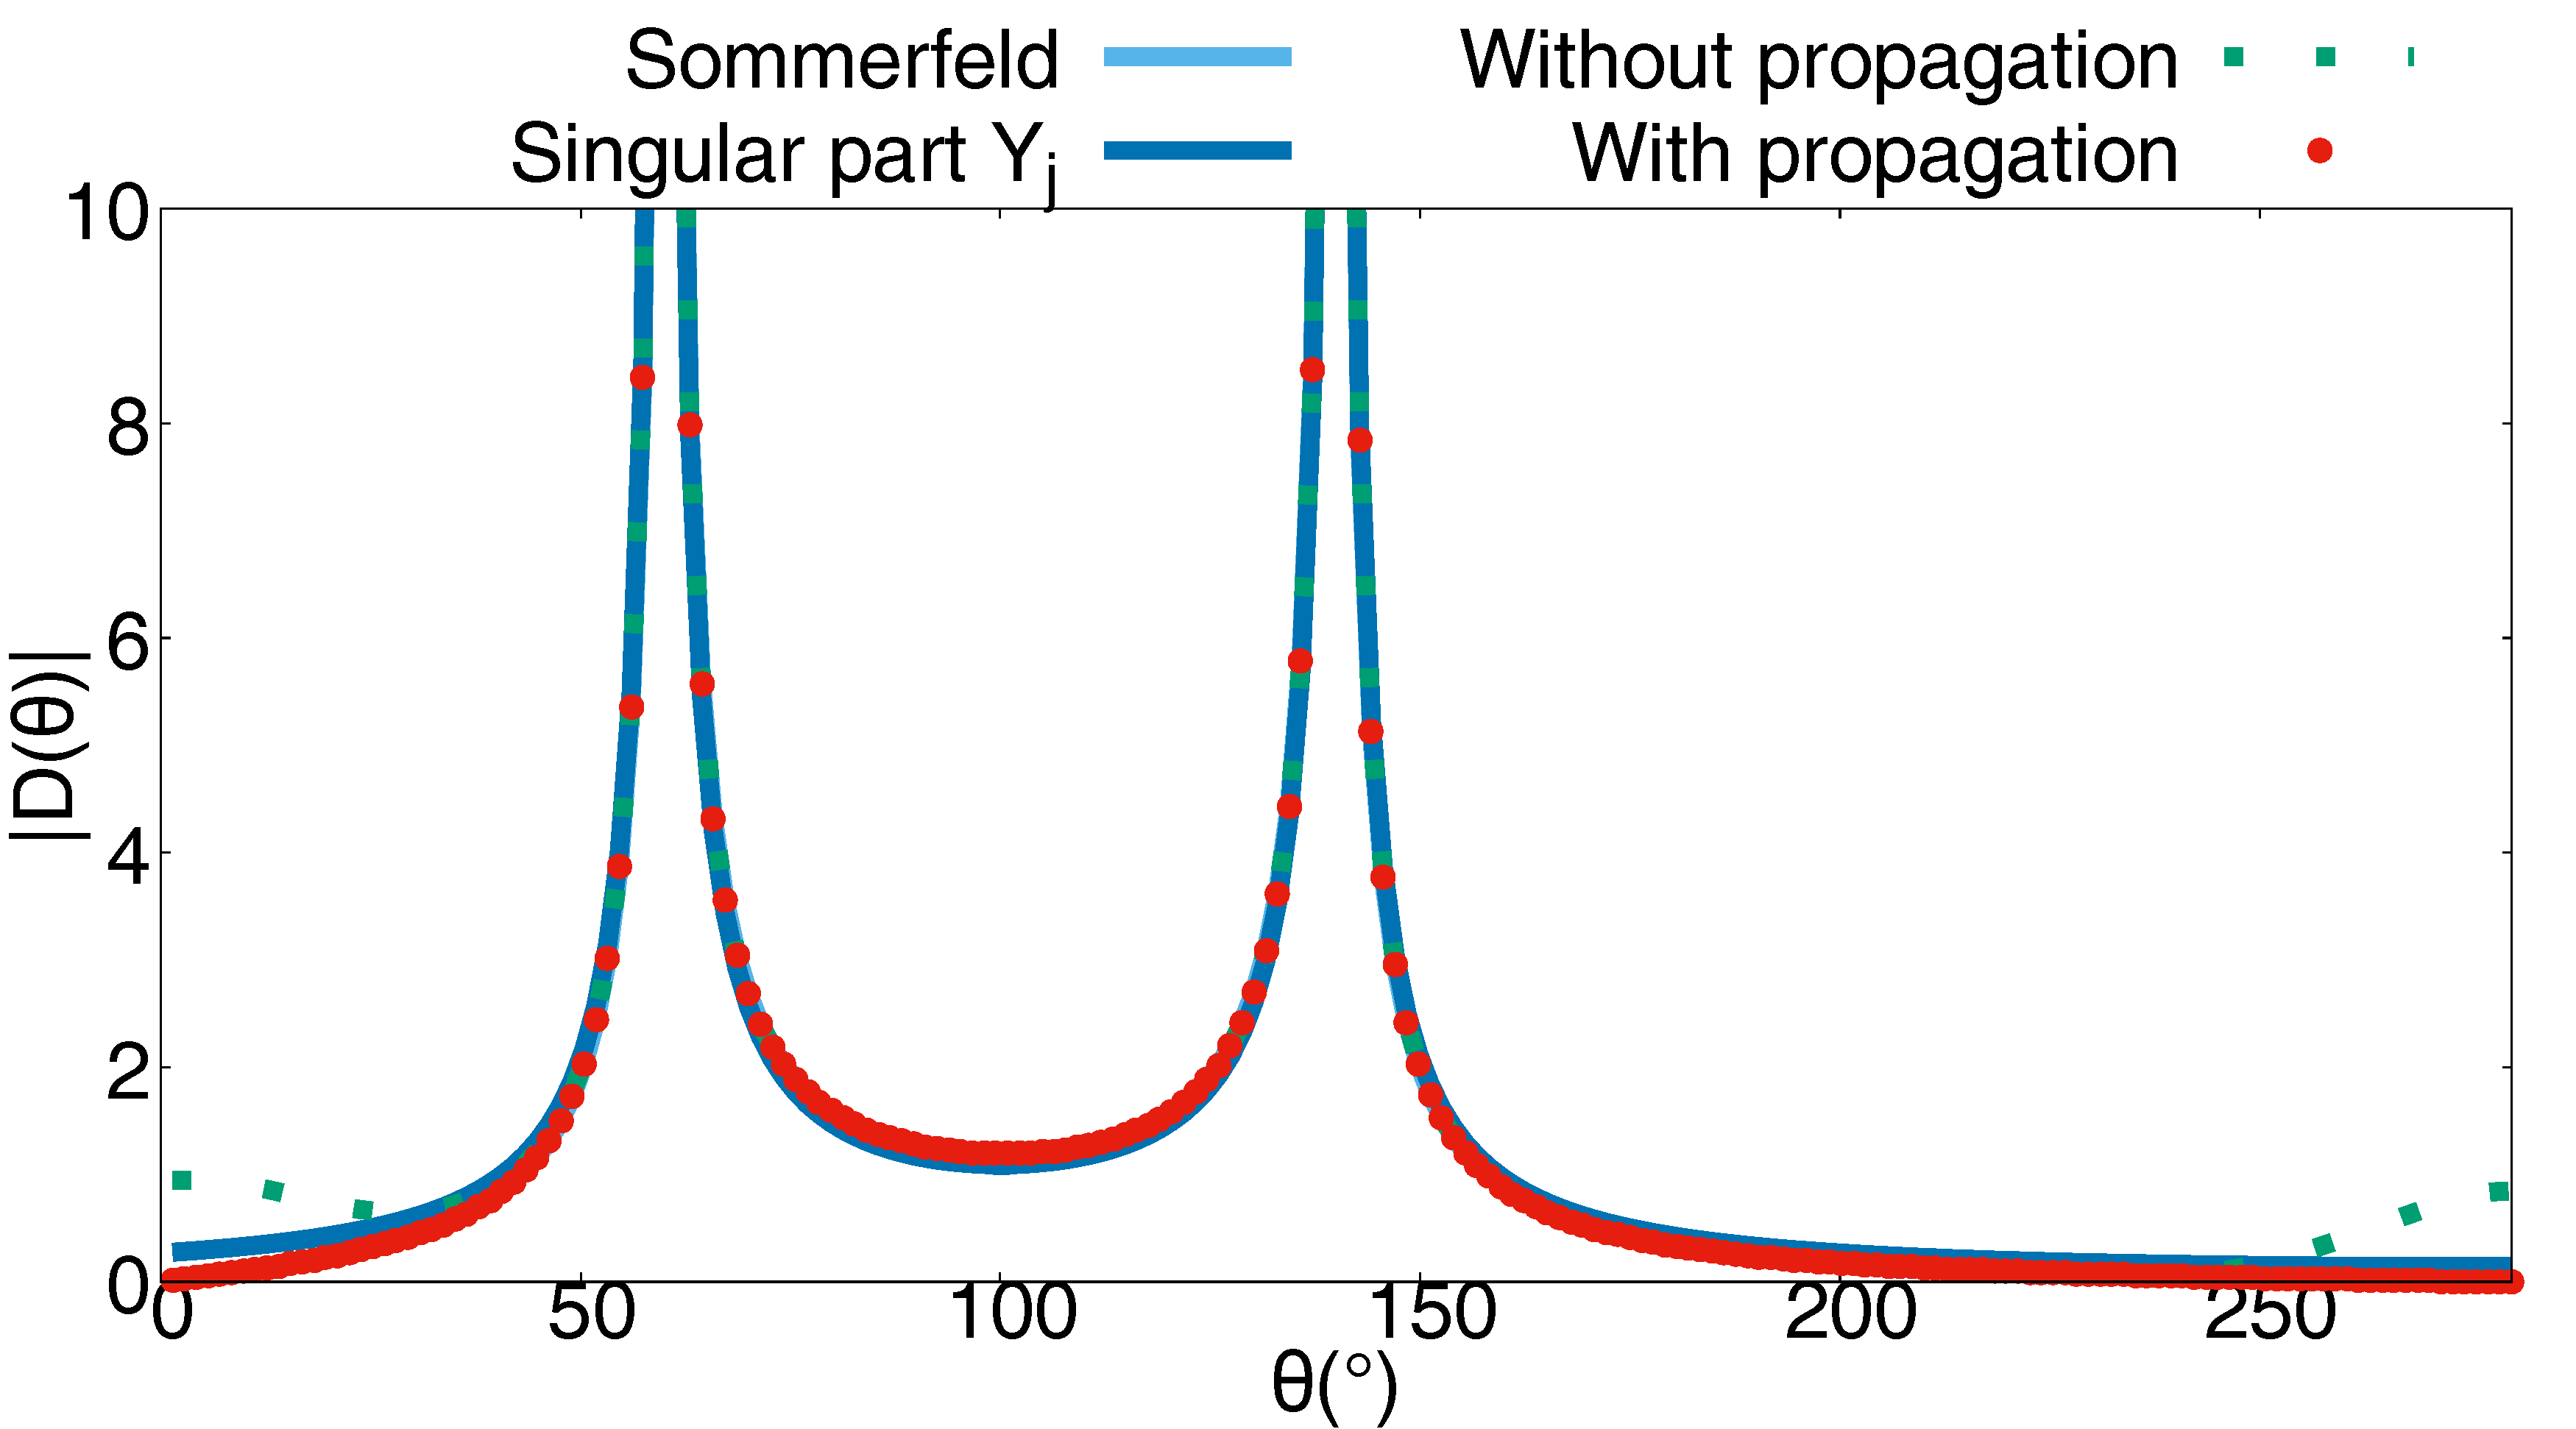
\includegraphics[width=\textwidth]{images/chapter2/Figure8c.pdf}
        \caption{$2\varphi = 280^o$, $\theta_{\rm inc} = 240^o$}
        \label{chapter5:figure12d}
    \end{subfigure}
\begin{subfigure}[b]{0.49\textwidth}
        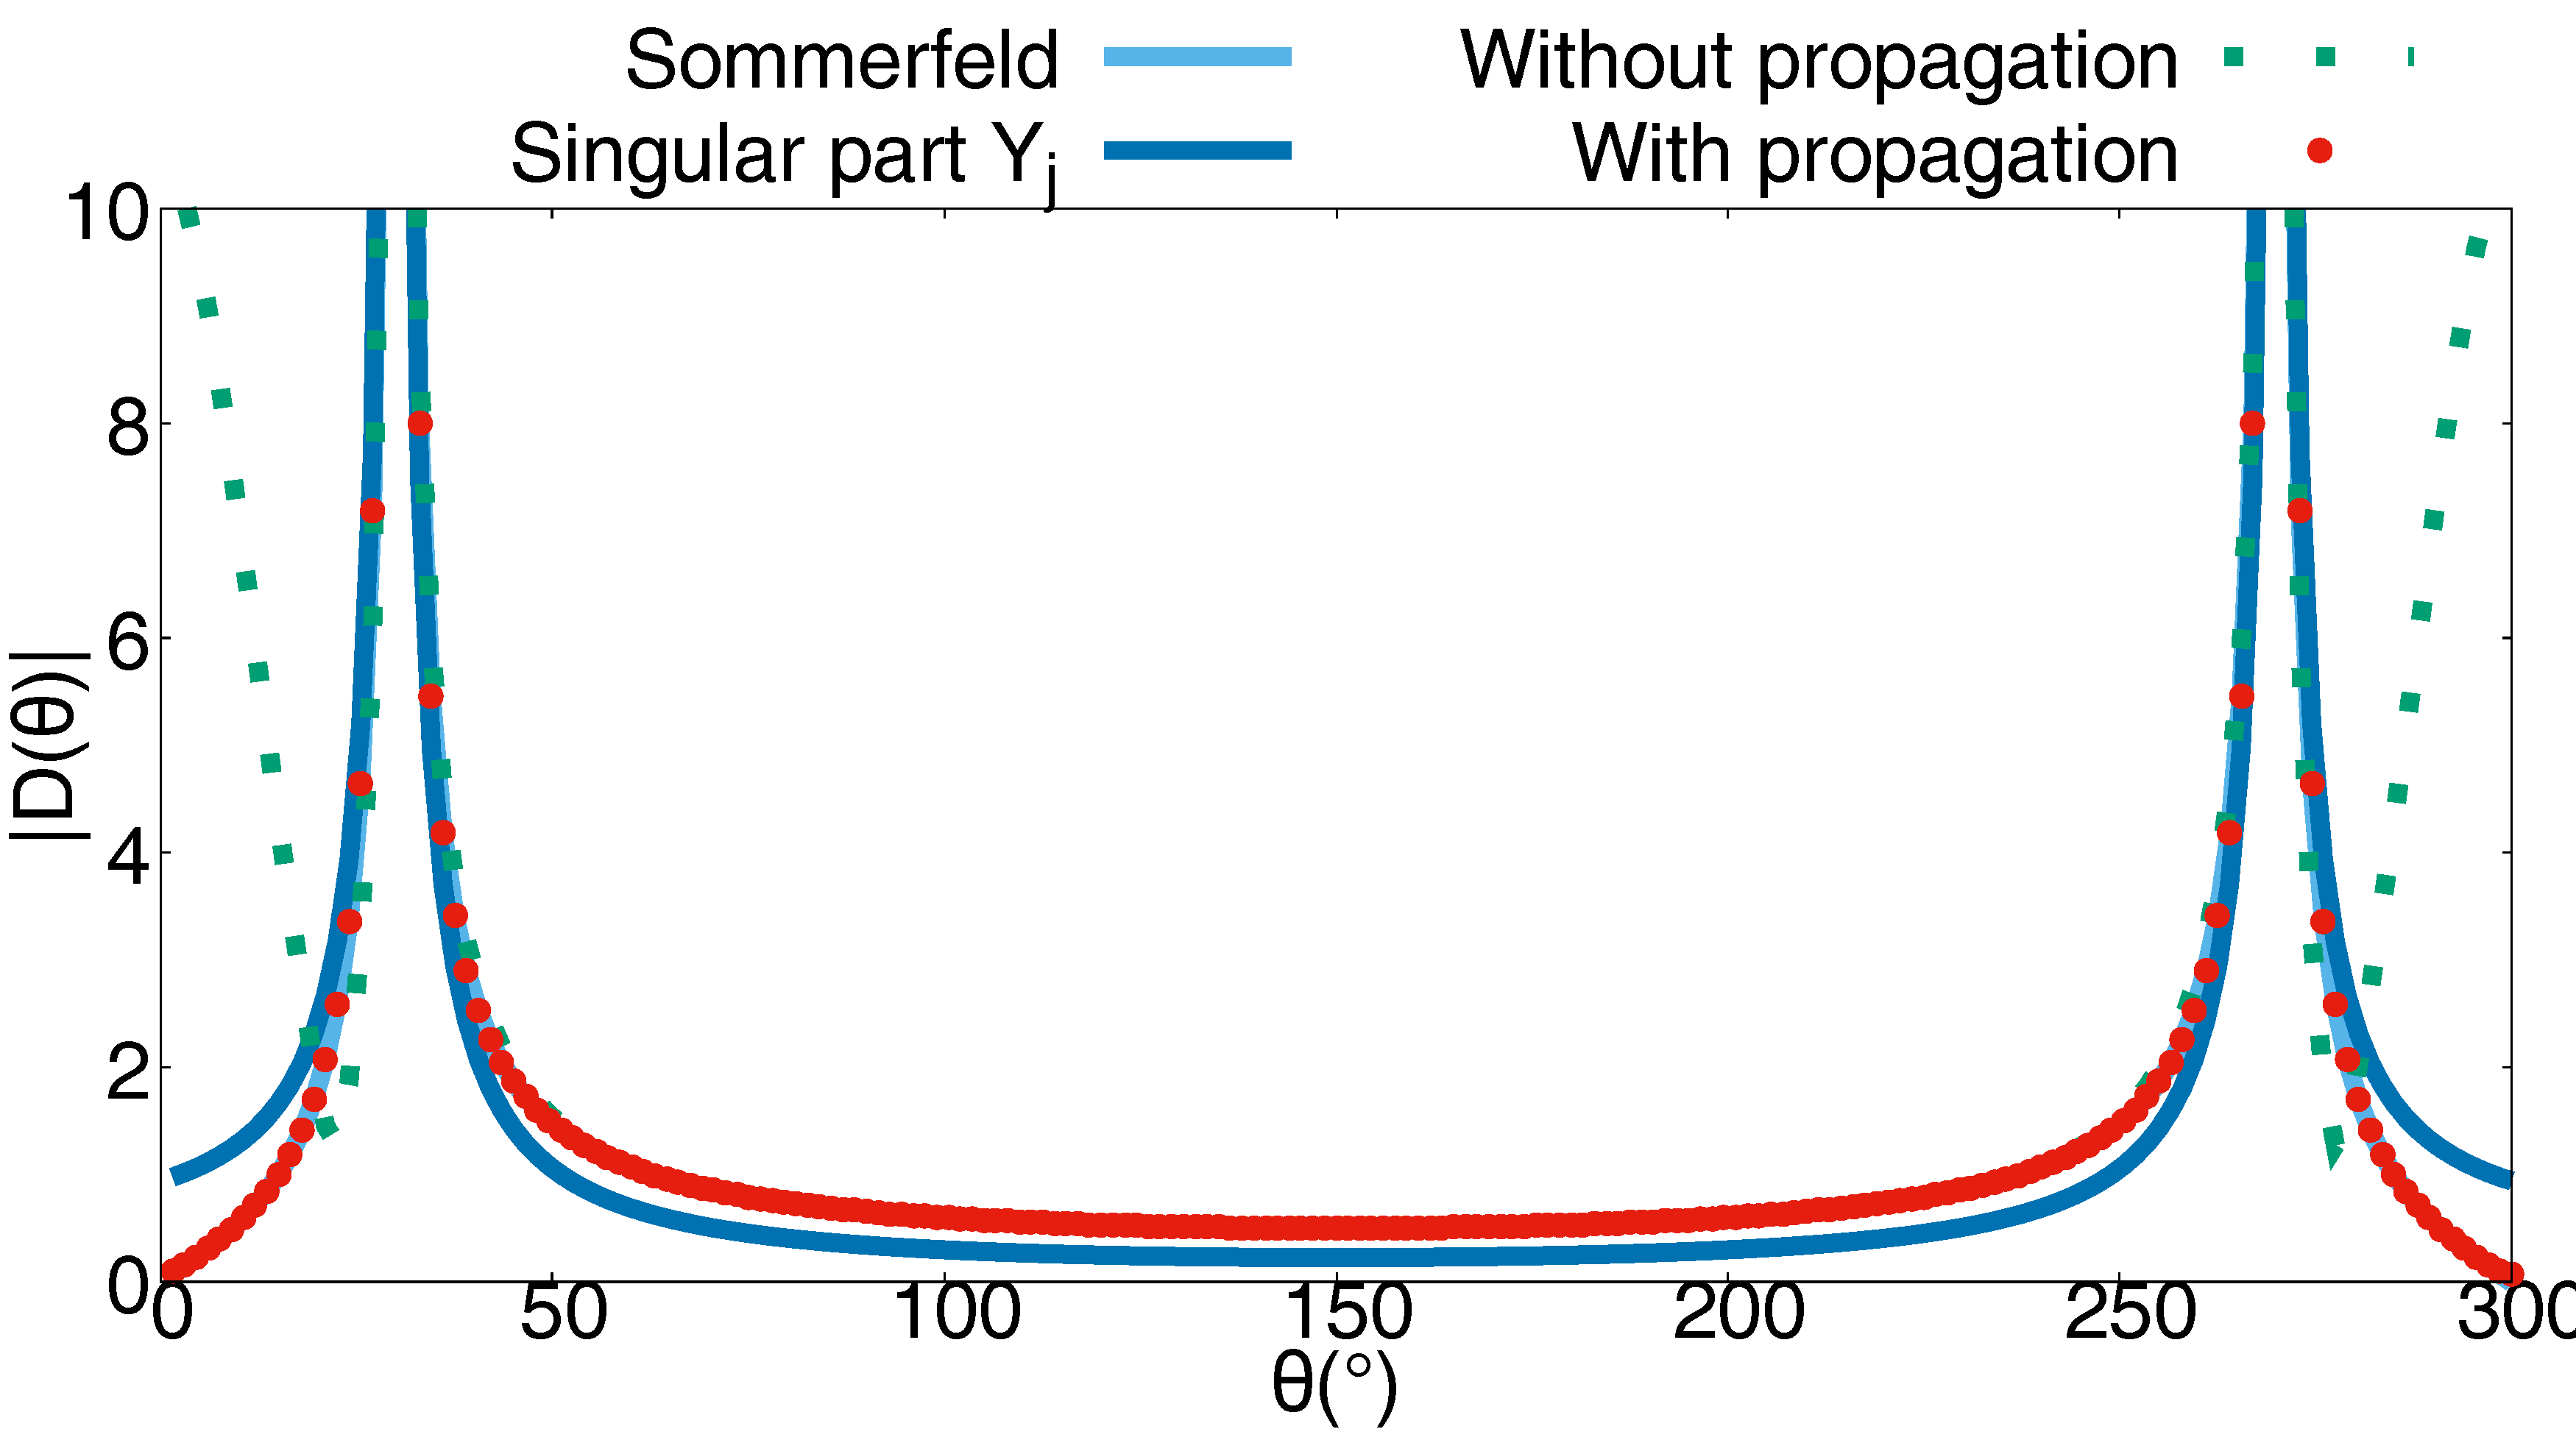
\includegraphics[width=\textwidth]{images/chapter2/Figure8d.pdf}
        \caption{$2\varphi = 300^o$, $\theta_{\rm inc} = 150^o$}
        \label{chapter5:figure12c}
    \end{subfigure}
\caption
[Diffraction coefficient computed with the recursive formula of spectral functions and with the Sommerfeld method, in the case of Dirichlet boundary conditions]
{Diffraction  coefficient computed with the spectral functions and with the Sommerfeld method, in the case of Dirichlet boundary conditions.}
\label{chapter5:figure12}
\end{figure}

In the case of Neumann boundary conditions, the initial system \eqref{Chapter5:Adimen_waveMotion} is replaced by the follwing :
\begin{equation}
\begin{cases}
(\triangle+1)v =  0 \quad \text{in } \Omega_f, \\
\partial v/\partial n =  -\partial h_{\rm inc}/\partial n \quad \quad \quad \text{on } F_j, \quad j=1,2
\end{cases},
\label{neuproblem}
\end{equation}
where n is the inward-pointing normal to the wedge faces. The spectral functions method can once again be applied following the same steps as for the Dirichlet boundary conditions. The details of the computation are not repeated here. Once again, a far-field evaluation of the diffraction, given by  \eqref{GTDCoeff_SF} is compared to the analytic expression of the diffraction coefficient given by Sommerfeld \cite{Sommerfeld}. The GTD approximation of this coefficient is also given by Keller \cite{GTD} :
\begin{align}
\label{GTDCoeff_Neu}
D^{\rm (Neu)}(\theta) = \dfrac{e^{i\frac{\pi}{4}}}{2N \sqrt{2\pi}}  \, \left[ \cot \left( \dfrac{\pi + (\theta + \theta_{\rm inc})}{2N} \right) + \cot \left( \dfrac{\pi - (\theta + \theta_{\rm inc})}{2N} \right) \right.   \nonumber \\
\left. + \cot \left( \dfrac{\pi + (\theta - \theta_{\rm inc})}{2N} \right) + \cot \left( \dfrac{\pi - (\theta - \theta_{\rm inc})}{2N} \right) \right] 
\end{align}
with $N=2\varphi/\pi$. The results are presented on Fig ~\ref{chapter5:figure13}.

\begin{figure}[h!]
\centering
\begin{subfigure}[b]{0.49\textwidth}
        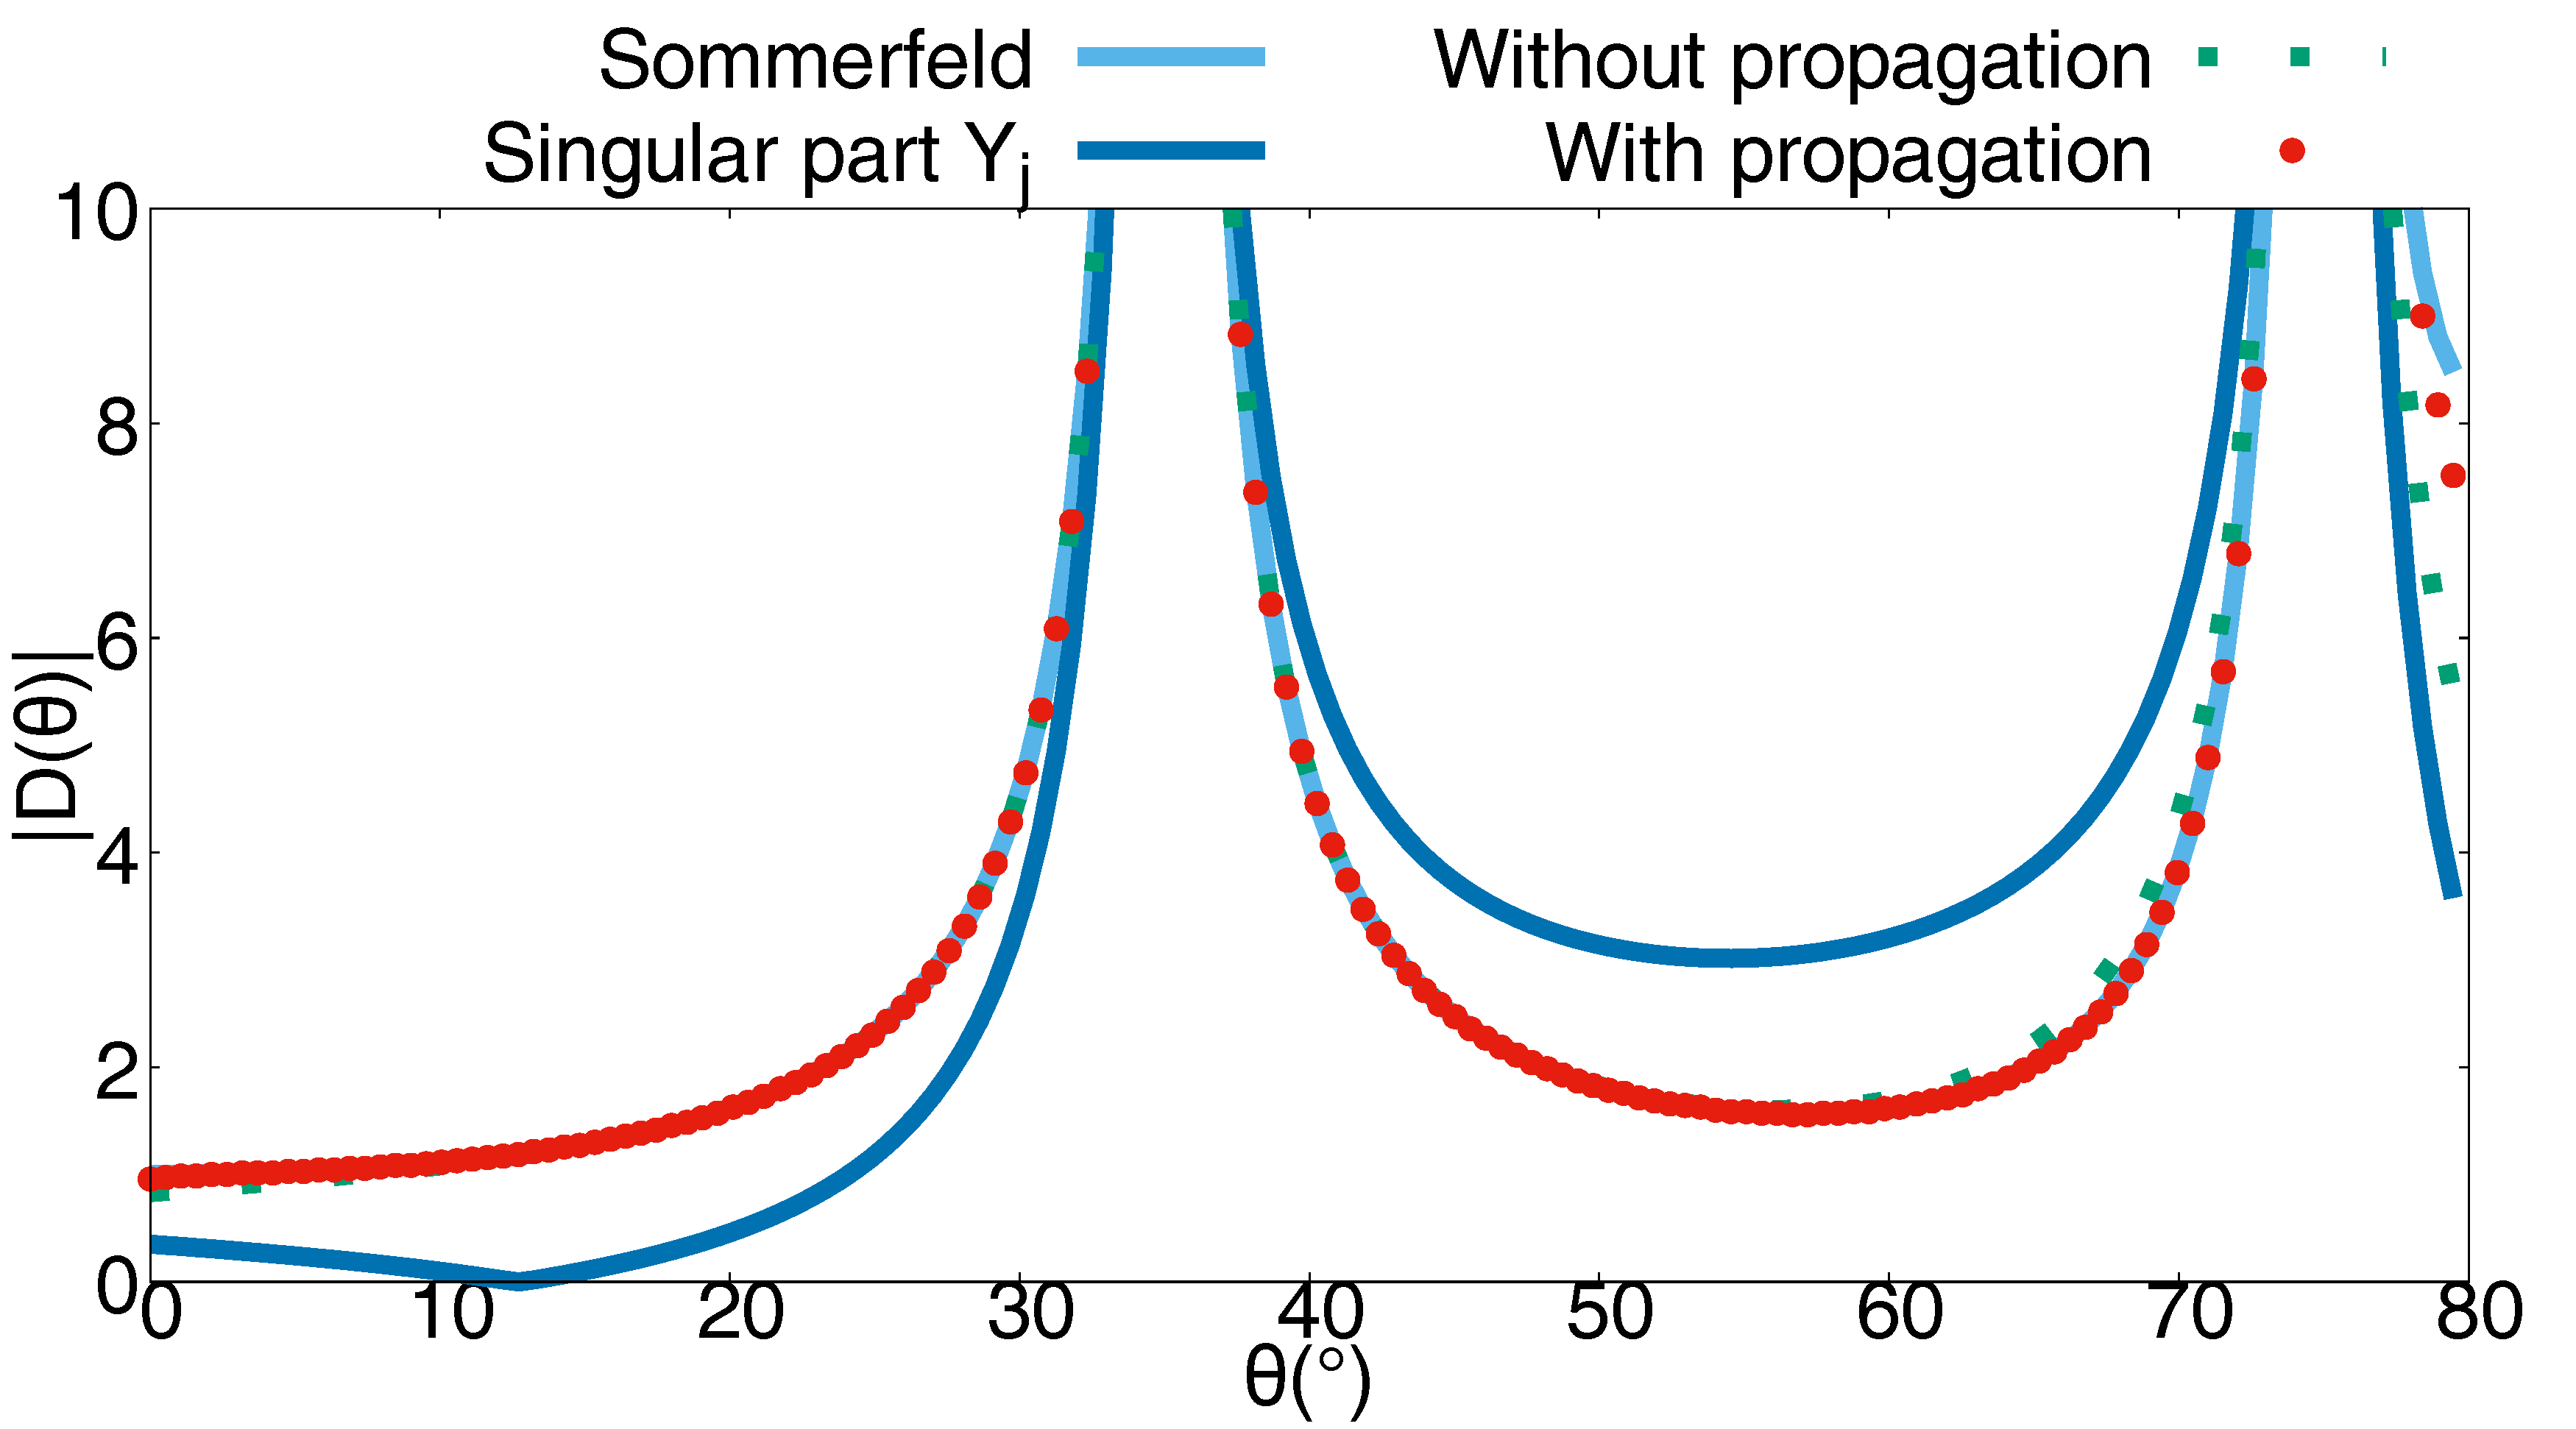
\includegraphics[width=\textwidth]{images/chapter2/Figure9a.pdf}
        \caption{$2\varphi = 80^o$, $\theta_{\rm inc} = 55^o$}
        \label{chapter5:figure13a}
    \end{subfigure}
\begin{subfigure}[b]{0.49\textwidth}
        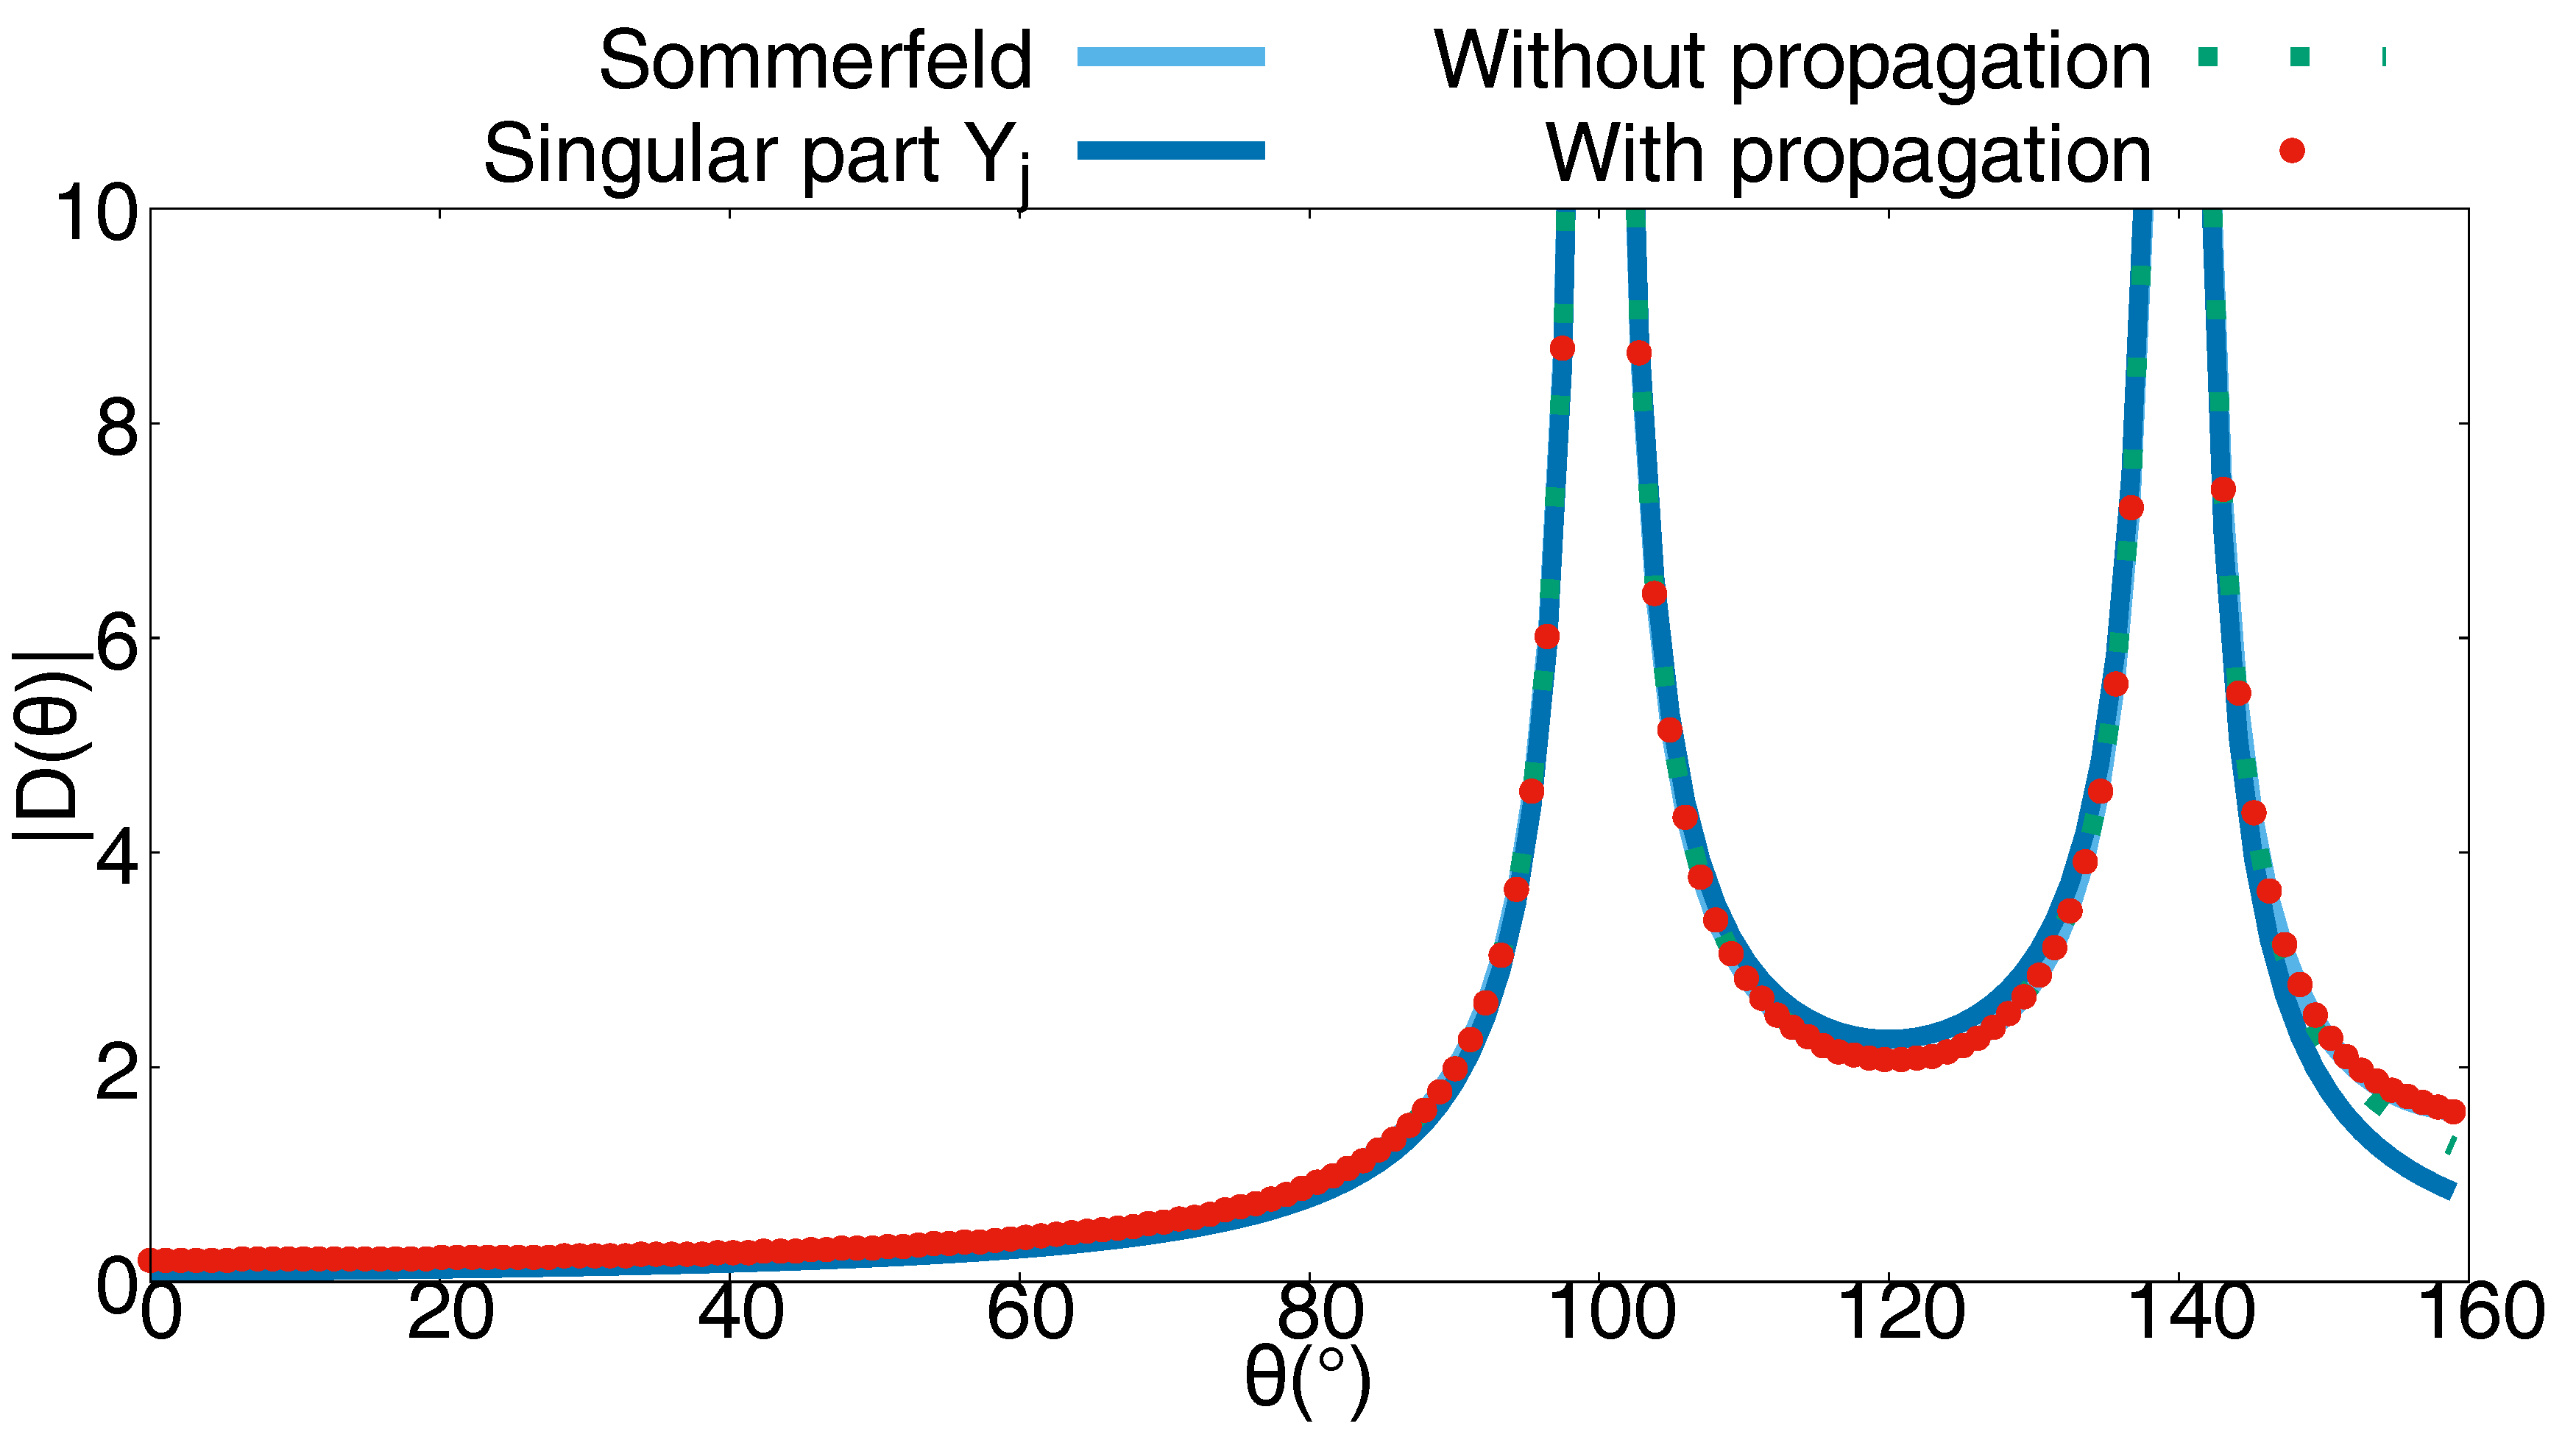
\includegraphics[width=\textwidth]{images/chapter2/Figure9b.pdf}
        \caption{$2\varphi = 160^o$, $\theta_{\rm inc} = 40^o$}
        \label{chapter5:figure13b}
    \end{subfigure}
\\
~\\
\begin{subfigure}[b]{0.49\textwidth}
        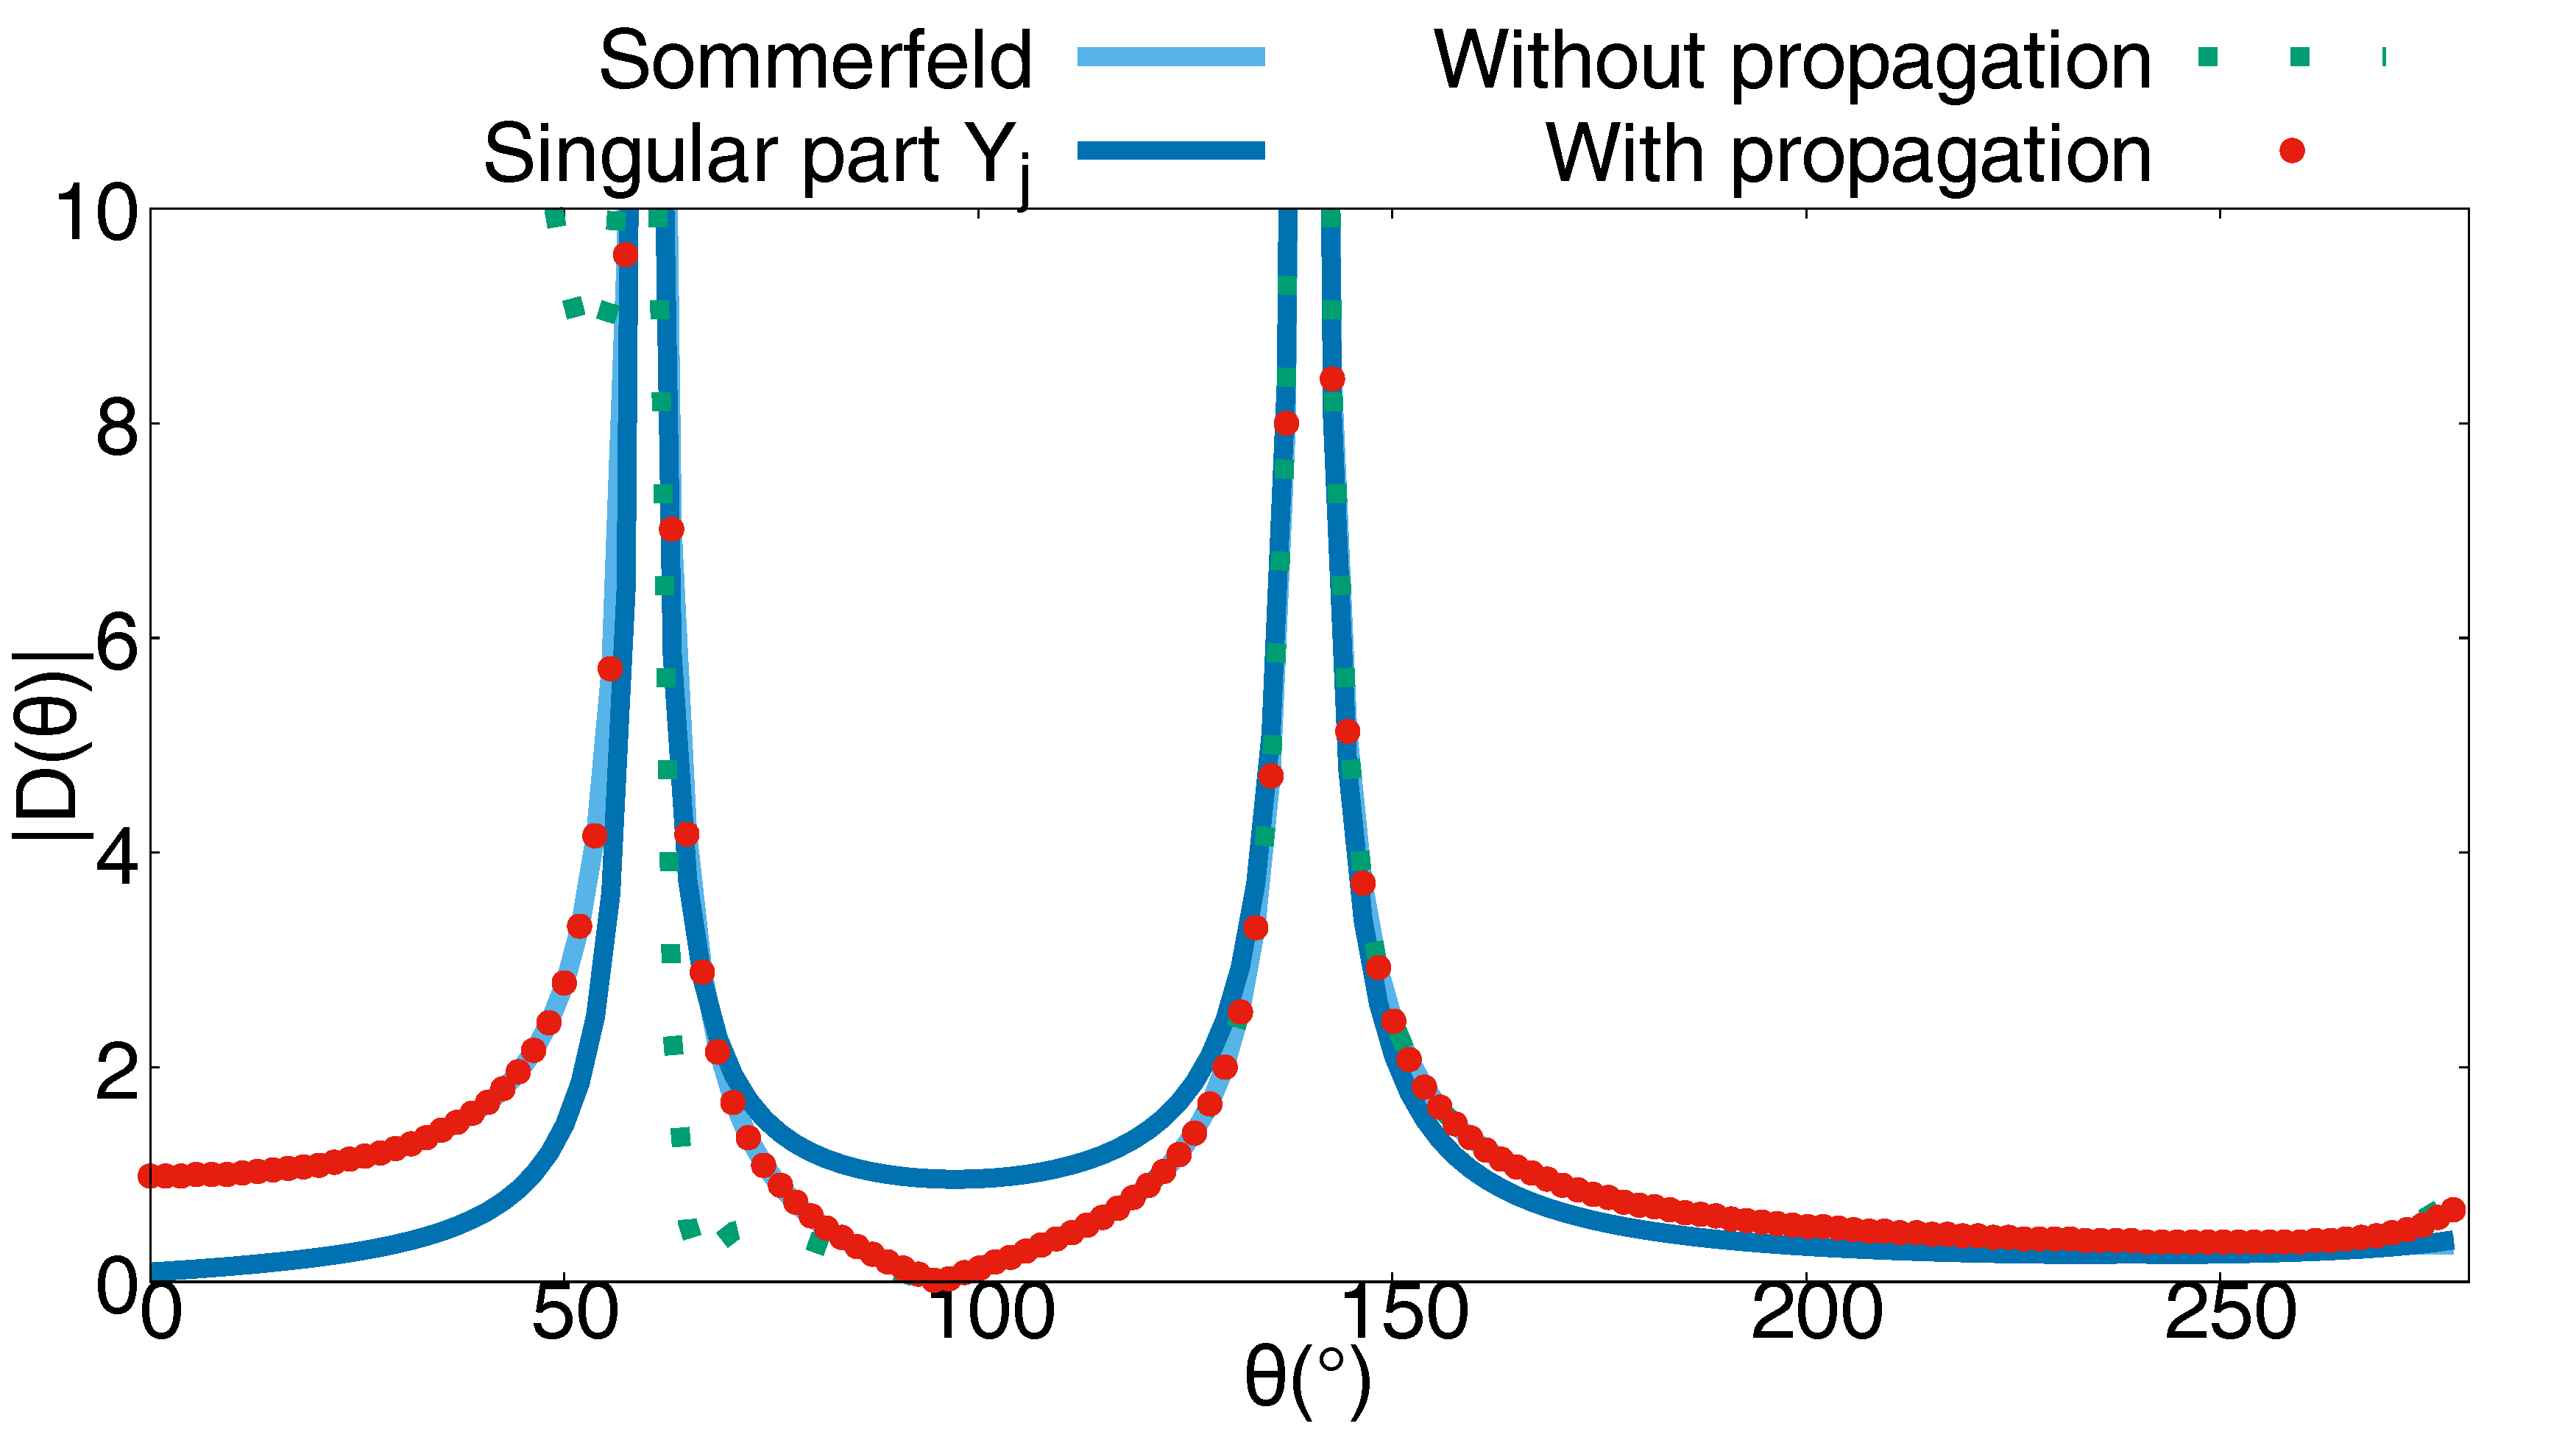
\includegraphics[width=\textwidth]{images/chapter2/Figure9c.pdf}
        \caption{$2\varphi = 280^o$, $\theta_{\rm inc} = 240^o$}
        \label{chapter5:figure13d}
    \end{subfigure}
\begin{subfigure}[b]{0.49\textwidth}
        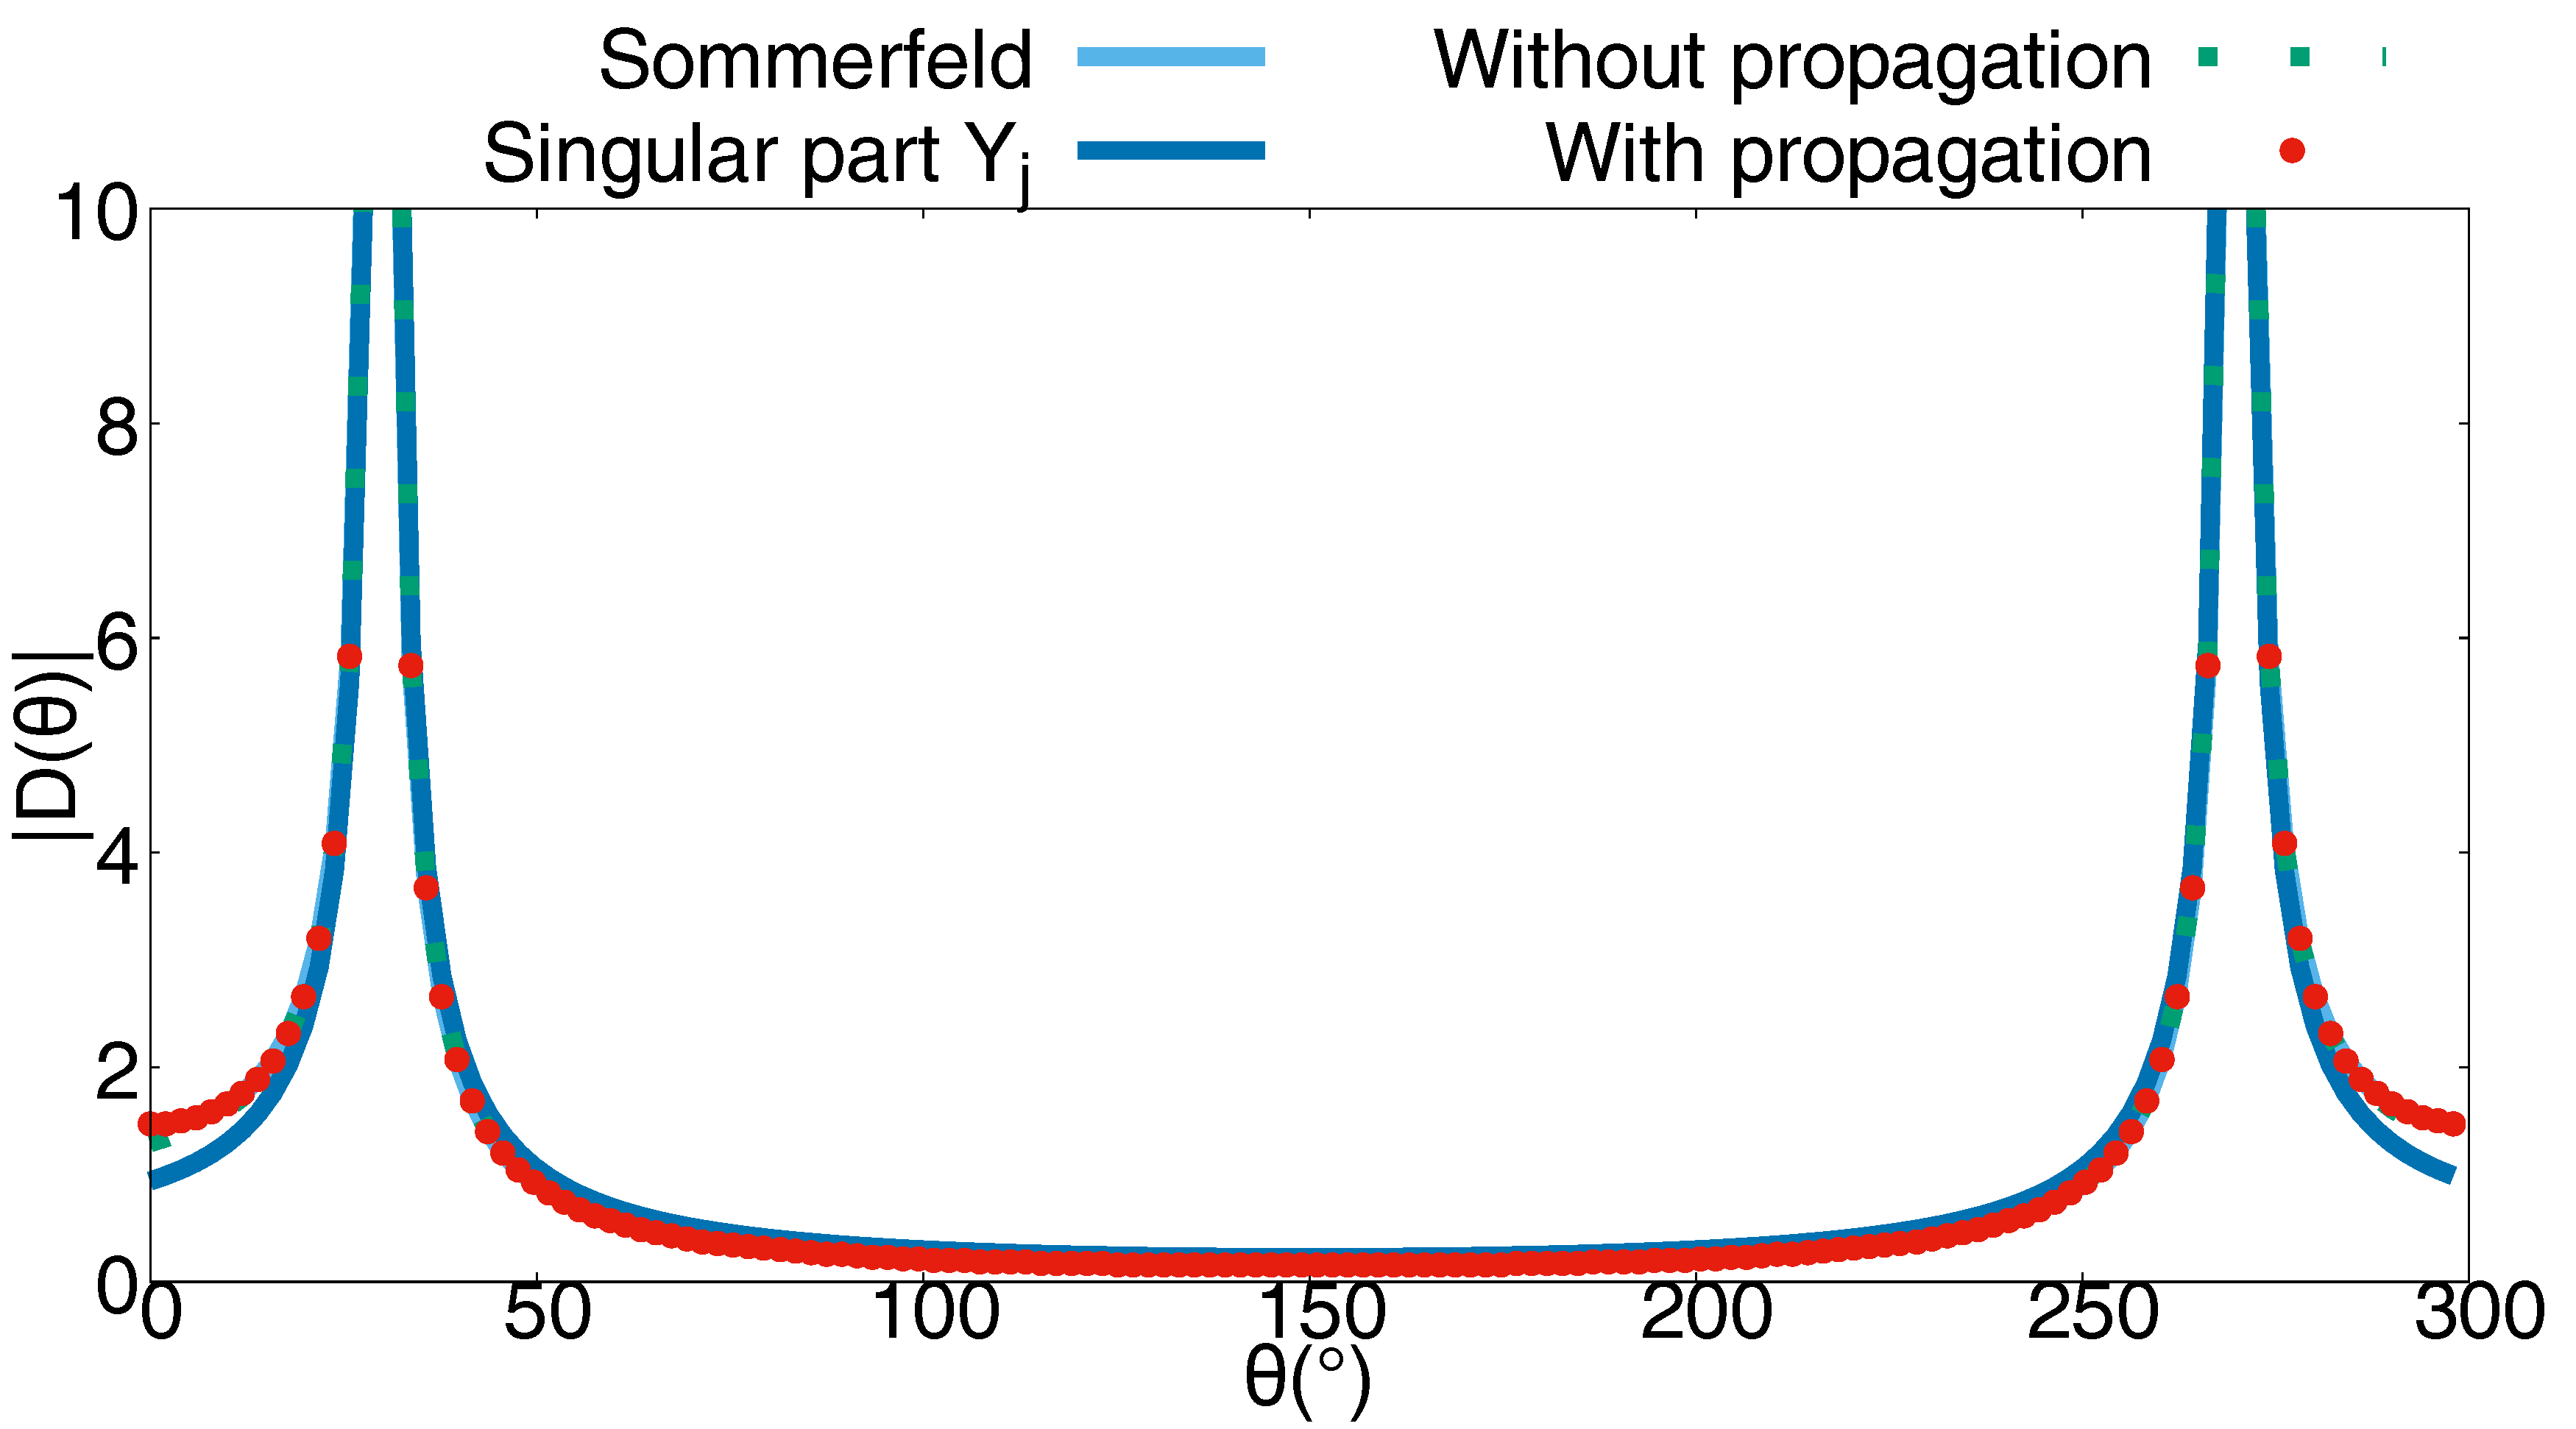
\includegraphics[width=\textwidth]{images/chapter2/Figure9d.pdf}
        \caption{$2\varphi = 300^o$, $\theta_{\rm inc} = 150^o$}
        \label{chapter5:figure13c}
    \end{subfigure}
\caption
[Diffraction  coefficient computed with the recursive formula of spectral functions and with the Sommerfeld method, in the case of Neumann boundary conditions]
{Diffraction  coefficient computed with the spectral functions and with the Sommerfeld method, in the case of Neumann boundary conditions.}
\label{chapter5:figure13}
\end{figure}


 In each of these figures, the continuous light blue line represents the modules of the diffraction coefficients obtained using the Sommerfeld integral method, the continuous dark blue line represents those obtained using the Spectral function singular part $Y_j$ alone, the short-dashed green line represents those obtained using the Spectral functions method without propagation of the solution and the red circles represent those obtained using the spectral functions method with propagation of the solution described in paragraph \ref{propag_sol}.

On Figs.~\ref{chapter5:figure12a},~\ref{chapter5:figure12b},~\ref{chapter5:figure13a} and ~\ref{chapter5:figure13b} the wedge angles are lower than $\pi$ and on figs.~\ref{chapter5:figure12c},~\ref{chapter5:figure12d},~\ref{chapter5:figure13c} and ~\ref{chapter5:figure13d} the wedge angles are greater than $\pi$. In all cases, it appears clearly that both the regular part of the solution and the recursive method are necessary to obtain optimal results. When both of these are included, diffraction coefficients obtained with Spectral functions are close to those of the Sommerfeld method. In addition, the run time to evaluate the diffraction coefficients in 250 different observation points, in each of the presented configurations, using an Intel(R) Xeon(R) CPU E3-1240 v3 is under 0.1 seconds for both methods. 

%
% Troisième chapitre
%\chapter{Conclusion}
Dans ce chapitre, nous concluons l'étude du chaos du rire.

\lipsum[26-27]
\section{Une section}
\lipsum[28-29]
\subsection{Une sous-section}
\lipsum[29-31]
\subsubsection{Une sous-sous-section}
\lipsum[31-35]
\paragraph{Un paragraphe}
\lipsum[36-38]
\paragraph{Un sous-paragraphe}
\lipsum[39-41]
\paragraph{Un autre sous-paragraphe}
\lipsum[39-41]
\paragraph{Un autre paragraphe}
\lipsum[36-38]
\subsubsection{Une autre sous-sous-section}
\lipsum[31-35]
\subsection{Une autre sous-section}
\lipsum[29-31]
\section{Une autre section}
\lipsum[28-29]

%
%
% Deuxième partie éventuelle
%\part{Le rire du chaos}
%
% Quatrième chapitre
%\chapter{Contexte du rire du chaos}
\epigraphhead[30]{\epigraph{La science a fait de nous des dieux avant même que
    nous méritions d'être des hommes.}{Jean Rostand}}

\lipsum[26-32]

%
% Cinquième chapitre
%\chapter{Développement}

Nous pouvons faire référence à des graphiques (très jolis au demeurant), comme
celui de la figure\vref{sin-x*sin-y}.
\lipsum[3-10]
\begin{figure}[ht]
  \centering
  \capstart
  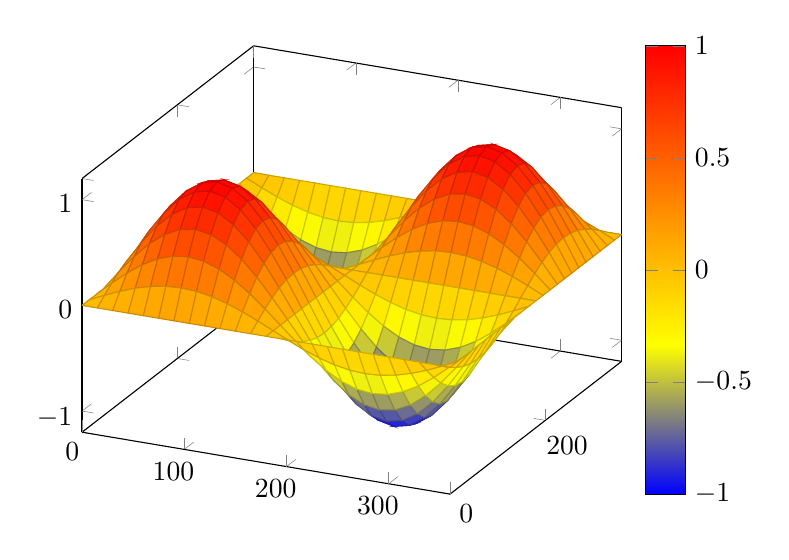
\begin{tikzpicture}
    \begin{axis}[colorbar]
      \addplot3[surf,domain=0:360]
      {sin(x)*sin(y)};
    \end{axis}
  \end{tikzpicture}
  \caption{Représentation graphique de la fonction $f:(x,y)\mapsto
    \sin x\times\sin y$}
  \label{sin-x*sin-y}
\end{figure}

%
% Sixième chapitre
%\chapter{Conclusion}
Dans ce chapitre, nous concluons l'étude du rire du chaos.

\lipsum[6-9]

%
% Chapitre  de conclusion (générale)
%%%%%%%%%%%%%%%%%%%%%%%%%%%%%%%%%%%%%%%%%%%%%%%%%%%%%%%%%%%%%%%%%%%%%%%%%%%%%%%
%\chapter*{Conclusion générale}
\lipsum[26-27]
\section{Une section de conclusion}
\lipsum[28-29]
\subsection{Une sous-section de conclusion}
\lipsum[29-31]
\subsubsection{Une sous-sous-section de conclusion}
\lipsum[31-35]
\paragraph{Un paragraphe de conclusion}
\lipsum[36-38]
\subparagraph{Un sous-paragraphe de conclusion}
\lipsum[39-41]
\subparagraph{Un autre sous-paragraphe de conclusion}
\lipsum[39-41]
\paragraph{Un autre paragraphe de conclusion}
\lipsum[36-38]
\subsubsection{Une autre sous-sous-section de conclusion}
\lipsum[31-37]
\subsection{Une autre sous-section de conclusion}
\lipsum[29-31]
\section{Une autre section de conclusion}
\lipsum[28-43]

%
% Liste des références bibliographiques
\printbibliography
%
%%%%%%%%%%%%%%%%%%%%%%%%%%%%%%%%%%%%%%%%%%%%%%%%%%%%%%%%%%%%%%%%%%%%%%%%%%%%%%%
% Début de la partie annexe éventuelle
%%%%%%%%%%%%%%%%%%%%%%%%%%%%%%%%%%%%%%%%%%%%%%%%%%%%%%%%%%%%%%%%%%%%%%%%%%%%%%%
\appendix
%
% Premier chapitre annexe (éventuel)
%\chapter{Documents juridiques}
\label{chap-juridique}

Cette partie regroupe les documents juridiques officiels.

\section{Licence sous laquelle est publié notre travail}
\label{sec-discours}

\lipsum[11-30]

\section{Transposition de la licence précédente en droit français}
\label{sec-autre-discours}

\lipsum[31-50]

%
% Deuxième chapitre annexe (éventuel)
%\chapter{Programmes informatiques}
\label{chap-listings}

Les listings suivants sont au cœur de notre travail.

\lstinputlisting[caption={Il est l'heure}]{annexes/programmes/heure.c}
\lstinputlisting[caption={Factorielle}]{annexes/programmes/factorielle.c}

%
\chapter{Calcul des intégrales $\int_{-1}^1 \frac{\lambda t+ \rho}{Q(t)}\, dt$ et $\int_{-1}^1 \frac{\eta t+ \psi}{P(t)}\, dt$ }
\label{Intégrale}
Avant de nous lancer dans le détail des calculs des coefficients des matrices $\mathbb{D}$ et $\mathbb{T}$, nous allons commencer par calculer deux intégrales élémentaires dont les valeurs seront utilisées dans toute la suite.
\section{Intégrale $\int_{-1}^1 \frac{\lambda t+ \rho}{Q(t)}\, dt$}
\label{calculIntQ}
On calcule :
\begin{equation*}
\int_{-1}^1 \frac{\lambda t+ \rho}{Q(t)}\, dt=\int_{-1}^1 \frac{\lambda t}{iat^2+2\nu t-ia}\,dt+\int_{-1}^1\frac{\rho}{ia(t-q_+)(t-q_-)}\,dt
\end{equation*}
Où on note $q_+,q_-$ les racines de Q. On a:
\begin{equation}
q_\pm=\frac{1}{a}(i\nu\pm\sqrt{a^2-\nu^2})
\label{q1q2}
\end{equation}

\begin{equation*}
\begin{split}
\int_{-1}^1 \frac{\lambda t+ \rho}{Q(t)}\, dt&=\int_{-1}^1 \frac{\frac{\lambda}{2ia} (2iat+2\nu)}{iat^2+2\nu t-ia}\,dt+(\rho-\frac{\lambda \nu}{ia})\int_{-1}^1\frac{1}{ia(t-q_+)(t-q_-)}\,dt\\
&=\frac{\lambda\pi}{2a}+\frac{1}{q_+-q_-}\left(\frac{\rho}{ia}+\frac{\lambda\nu}{a^2}\right)\int_{-1}^1\left(\frac{1}{t-q_+}-\frac{1}{t-q_-}\right)\,dt
\end{split}
\end{equation*}
On réinjecte les expressions de $q_\pm$ données par (\ref{q1q2}):
\begin{equation*}
\begin{split}
\int_{-1}^1 \frac{\lambda t+ \rho}{Q(t)}\, dt&=\frac{\lambda\pi}{2a}+\frac{1}{2\sqrt{a^2-\nu^2}}\left(\frac{\lambda\nu}{a}-i\rho\right)\log\left(\frac{(1-q_+)(1+q_-)}{(1-q_-)(1+q_+)}\right)\\
&=\frac{\lambda\pi}{2a}+\frac{1}{2\sqrt{a^2-\nu^2}}\left(\frac{\lambda\nu}{a}-i\rho\right)\log\left(\frac{-\nu^2-(a-\sqrt{a^2-\nu^2})^2}{-\nu^2-(a+\sqrt{a^2-\nu^2})^2}\right)\\
&=\frac{\lambda\pi}{2a}+\frac{1}{2\sqrt{a^2-\nu^2}}\left(\frac{\lambda\nu}{a}-i\rho\right)\log\left(\frac{-a+\sqrt{a^2-\nu^2}}{-a-\sqrt{a^2-\nu^2}}\right)\\
&=\frac{\lambda\pi}{2a}+\frac{1}{\nu\sqrt{\frac{a^2}{\nu^2}-1}}\left(i\rho-\frac{\lambda\nu}{a}\right)\log\left(\frac{a}{\nu}+\sqrt{\frac{a^2}{\nu^2}-1}\right)
\end{split}
\end{equation*}
Soit finalement :
\begin{equation}
\int_{-1}^1 \frac{\lambda t+ \rho}{Q(t)}\, dt=\frac{\lambda}{\nu}\mbox{sog}(\frac{a}{\nu})+i\frac{\rho}{\nu}\mbox{rog}(\frac{a}{\nu})
\label{intQ}
\end{equation}
On a défini la fonction suivante, pour $a>1$
\begin{equation}
\mbox{rog}(a)=\int_{-1}^1\frac{dx}{a(1-x^2)+2ix}=\frac{1}{\sqrt{a^2-1}}\log(a+\sqrt{a^2-1})
\label{defrog}
\end{equation}
La branche de coupure de la racine carrée est le long de l'axe des réels négatifs. On definit ensuite :
\begin{equation}
\mbox{sog}(a)=\frac{1}{a}\left(\frac{\pi}{2}-\mbox{rog}(a)\right)
\label{defsog}
\end{equation}
\section{Intégrale $\int_{-1}^1 \frac{\eta t+ \psi}{P(t)}\, dt$}
\label{calculintP}
On calcule :
\begin{equation*}
\int_{-1}^1 \frac{\eta t+ \psi}{P(t)}\, dt = \int_{-1}^1 \frac{\eta t}{(\nu\sin\tilde{\varphi}-b)t^2-2i\nu t\cos\tilde{\varphi}+\nu\sin\tilde{\varphi}+b}\,dt +\int_{-1}^1 \frac{\psi}{(\nu\sin\tilde{\varphi}-b)(t-p_+)(t-p_-)}\, dt
\end{equation*}
Où on note $p_+,p_-$ les racines de $P$. On a :
\begin{equation}
p_\pm=\frac{\nu i \cos\tilde{\varphi}\pm \sqrt{b^2-\nu^2}}{\nu\sin\varphi-b}
\label{p1p2}
\end{equation}
\begin{equation*}
\begin{split}
\int_{-1}^1 \frac{\eta t+ \psi}{P(t)}\, dt =& \int_{-1}^1 \frac{\frac{\eta}{2(\nu\sin\tilde{\varphi}-b)}(2(\nu\sin\tilde{\varphi}-b)t-2i\nu\cos\tilde{\varphi})}{(\nu\sin\tilde{\varphi}-b)t^2-2i\nu t\cos\tilde{\varphi}+\nu\sin\tilde{\varphi}+b}\,dt\\
&+(\psi+\frac{\eta i\nu\cos\tilde{\varphi}}{\nu\sin\tilde{\varphi}-b})\int_{-1}^1 \frac{dt}{(\nu\sin\tilde{\varphi}-b)(t-p_+)(t-p_-)}\\
=&\frac{i\eta}{\nu\sin\tilde{\varphi}-b}(\tilde{\varphi}-\frac{\pi}{2})\\
&+\frac{1}{p_+-p_-}\left(\frac{\psi}{\nu\sin\tilde{\varphi}-b}+\frac{\eta i\nu\cos\tilde{\varphi}}{(\nu\sin\tilde{\varphi}-b)^2}\right)\int_{-1}^1 \left(\frac{1}{t-p_+}-\frac{1}{t-p_-}\right)\,dt\\
\end{split}
\end{equation*}
On réinjecte les expressions de $p_\pm$ données par (\ref{p1p2}) :
\begin{equation*}
\begin{split}
\int_{-1}^1 \frac{\eta t+ \psi}{P(t)}\, dt =&\frac{i\eta}{\nu\sin\tilde{\varphi}-b}(\tilde{\varphi}-\frac{\pi}{2})+\frac{1}{2\sqrt{b^2-\nu^2}}\left(\psi+\frac{\eta i\nu\cos\tilde{\varphi}}{\nu\sin\tilde{\varphi}-b}\right)\log\left(\frac{(1-p_+)(1+p_-)}{(1-p_-)(1+p_+)}\right)\\
=&\frac{i\eta}{\nu\sin\tilde{\varphi}-b}(\tilde{\varphi}-\frac{\pi}{2})\\
&+\frac{1}{2\sqrt{b^2-\nu^2}}\left(\psi+\frac{\eta i\nu\cos\tilde{\varphi}}{\nu\sin\tilde{\varphi}-b}\right)\log\left(\frac{-\nu^2\cos^2\tilde{\varphi}-(\nu\sin\tilde{\varphi}-b-\sqrt{b^2-\nu^2})^2}{-\nu^2\cos^2\tilde{\varphi}-(\nu\sin\tilde{\varphi}-b+\sqrt{b^2-\nu^2})^2}\right)\\
=&\frac{i\eta}{\nu\sin\tilde{\varphi}-b}(\tilde{\varphi}-\frac{\pi}{2})+\frac{1}{2\sqrt{b^2-\nu^2}}\left(\psi+\frac{\eta i\nu\cos\tilde{\varphi}}{\nu\sin\tilde{\varphi}-b}\right)\log\left(\frac{b+\sqrt{b^2-\nu^2}}{b-\sqrt{b^2-\nu^2}}\right)\\
=&\frac{i\eta}{\nu\sin\tilde{\varphi}-b}(\tilde{\varphi}-\frac{\pi}{2})+\frac{1}{\nu\sqrt{\frac{b^2}{\nu^2}-1}}\left(\psi+\frac{\eta i\nu\cos\tilde{\varphi}}{\nu\sin\tilde{\varphi}-b}\right)\log\left(\frac{b}{\nu}+\sqrt{\frac{b^2}{\nu^2}-1}\right)
\end{split}
\end{equation*}
Finalement :
\begin{equation}
\int_{-1}^1 \frac{\eta t+ \psi}{P(t)}\, dt =\frac{i\eta}{\nu\sin\tilde{\varphi}-b}\lbrack\tilde{\varphi}-\frac{\pi}{2}+\cos\tilde{\varphi} \mbox{rog}(\frac{b}{\nu})\rbrack+\frac{\psi}{\nu}\mbox{rog}(\frac{b}{\nu})
\label{intP}
\end{equation}

\chapter{Computation details for the coefficients of matrix $\mathbb{D}(a,b)$}
\label{matD}
In each chapter of this manuscript, a matrix $\mathbb{D}$ appears, the coefficients of which must be determined analytically. These coefficients are linear combinations of integrals noted $I_1^*$ to $I_5^*$. In this appendix, these integrals are defined and the details of their computation is given. Finally, expressions of the coefficients of matrix $\mathbb{D}$ in the acoustic case and 2D and 3D elastic cases are given, with respect to integrals $I_1^*$ to $I_5^*$. In all the following, $\nuti \in \{ 1,\nu_T,\nuti_L,\nuti_T \}$.

\section{Integral $I_1^*$}
\label{calcI1}
Integral $I_1^*$ is defined by :
\begin{equation}
\label{defI1}
I_1^*=\int_{-\infty}^{+\infty} \frac{y}{(y+ib)(y-ia)\sqrt{\nuti^2+y^2}}\,dy
\end{equation}
When $a+b \neq 0$, we have the simple elements decomposition :
\begin{equation}
\frac{y}{(y+ib)(y-ia)}=\frac{1}{a+b} \left( \frac{b}{y+ib}+\frac{a}{y-ia} \right), 
\label{decomp2}
\end{equation}
which leads to
\begin{equation}
I_1^*= \frac{1}{a+b} \left( \int_{-\infty}^{+\infty} \frac{b}{(y+ib)\sqrt{\nuti^2+y^2}} \,dy +\int_{-\infty}^{+\infty} \frac{a}{(y-ia)\sqrt{\nuti^2+y^2}} \,dy \right)
\end{equation}
In each of these integrals, the following variable change is applied :
\begin{equation}
\begin{split}
 y&=2\nuti \frac{t}{1-t^2} \\
\sqrt{\nuti^2+y^2}&=\nuti\left( \frac{1+t^2}{1-t^2} \right)  \\
 dy&= 2\nuti \frac{1+t^2}{(1-t^2)^2}dt 
\end{split}
\label{changevar}
\end{equation}
Yielding
\begin{equation}
\int_{-\infty}^{+\infty} \frac{dy}{(y-ia)\sqrt{\nuti^2+y^2}}=\int_{-1}^1\frac{2\,dt}{2\nuti t-ia(1-t^2)}
\end{equation}
Finally, formula \eqref{intQ} is applied :
\begin{equation}
I_1^*=\frac{2ia}{(a+b)\nuti}\mbox{rog}(a/\nuti)-\frac{2ib}{(a+b)\nuti}\mbox{rog}(b/\nuti)
\label{valI1}
\end{equation}

\section{Integral $I_2^*$}
\label{calcI2}
Integral $I_2^*$ is defined by :
\begin{equation}
I_2^*=  \int_{-\infty}^{+\infty} \frac{y\sqrt{\nuti^2+y^2}}{(y+ib)(y-ia)}\, dy
\label{defI2}
\end{equation}
Note that
\begin{equation*}
\begin{split}
I_2^*&=\nuti^2 \int_{-\infty}^{+\infty}  \frac{y}{(y+ib)(y-ia)\sqrt{\nuti^2+y^2}}\,dy+ \int_{-\infty}^{+\infty} \frac{y^3}{(y+ib)(y-ia)\sqrt{\nuti^2+y^2}} \, dy\\
I_2^*&=\nuti^2 I_1^*+I_3^*,
\end{split}
\end{equation*}
where integrals $I_1^*$ and $I_3^*$ are defined by equations \eqref{defI1} and \eqref{defI3} and their expressions are given by \eqref{valI1} and \eqref{valI3} respectively.

\section{Integral $I_3^*$}
\label{calcI3}
Integral $I_3^*$ is defined by :
\begin{equation}
I_3^*=\int_{-\infty}^{+\infty} \frac{y^3}{(y+ib)(y-ia)\sqrt{\nuti^2+y^2}} \,dy
\label{defI3}
\end{equation}
The simple elements decomposition \eqref{decomp2} leads to
\begin{equation}
I_3^*=\frac{b}{a+b}\int_{-\infty}^{+\infty} \frac{y^2}{(y+ib)\sqrt{\nuti^2+y^2}} \, dy +\frac{a}{a+b}\int_{-\infty}^{+\infty} \frac{y^2}{(y-ia)\sqrt{\nuti^2+y^2}} \, dy
\label{decompI3}
\end{equation}

Once again, variable change \eqref{changevar} is applied
\begin{equation}
 \int_{-\infty}^{+\infty} \frac{y^2}{(y-ia)\sqrt{\nuti^2+y^2}} \,dy = \int_{-1}^1 \frac{8\nuti^2t^2}{(1-t^2)^2(2\nuti t -ia(1-t^2))} \, dt
\end{equation}

The integrated functions can be decomposed as such :
\begin{equation}
\frac{t^2}{(1-t^2)^2(2\nuti t -ia(1-t^2))}=\frac{\alpha}{1-t}+\frac{\beta}{1+t}+ \frac{\gamma}{(1-t)^2}+\frac{\delta}{(1+t)^2} +\frac{\lambda t + \rho }{2\nuti t-ia(1-t^2)},
\label{elemsimpl3}
\end{equation}
where the coefficients $\alpha,\beta,\gamma,\delta,\lambda,\rho$ will be determined in the sequel.

To determine $\gamma$, \eqref{elemsimpl3} is multiplied by $(1-t)^2$ and the result is evaluated at $t=1$. Similarly, $\delta$ is determined by multiplying \eqref{elemsimpl3} by $(1+t)^2$ and evaluating the result at $t=-1$ :
\begin{subequations}
\begin{equation}
\gamma=\frac{1}{8\nuti}
\end{equation}
\begin{equation}
\delta = -\frac{1}{8\nuti}
\end{equation}
\end{subequations}

The remaining terms are
\begin{equation}
\begin{split}
\frac{\alpha}{1-t}+\frac{\beta}{1+t}&+ \frac{\lambda t + \rho }{2\nuti t-ia(1-t^2)}\\  
~\\
&=\frac{t^2}{(1-t^2)^2(2\nuti t -ia(1-t^2))}-\frac{1}{8\nuti(1-t)^2}+\frac{1}{8\nuti(1+t)^2}  \\
~\\
&=\frac{8\nuti t^2-(1+t)^2(2\nuti t-ia(1-t^2))+(1-t)^2(2\nuti t-ia(1-t^2))}{8\nuti(1-t^2)^2(2\nuti_*-ia(1-t^2))}\\
~\\
&=\frac{iat}{2\nuti(1-t^2)(2\nuti t-ia(1-t^2))}
\end{split}
\end{equation}

To determine $\alpha$, \eqref{elemsimpl3} is multiplied by $(1-t)$ and the result is evaluated at $t=1$. Similarly, $\beta$ is determined by multiplying \eqref{elemsimpl3} by $(1+t)$ and evaluating the result at $t=-1$ :
\begin{subequations}
\begin{equation}
\alpha=\frac{ia}{8\nuti^2}
\end{equation}
\begin{equation}
\beta=\frac{ia}{8\nuti^2}
\end{equation}
\end{subequations}

The remaining term is
\begin{equation}
\begin{split}
 \frac{\lambda t + \rho }{2\nuti t-ia(1-t^2)} &=\frac{iat}{2\nuti(1-t^2)(2\nuti-ia(1-t^2))} -\frac{ia}{8\nuti^2(1-t)}-\frac{ia}{8\nuti^2(1+t)} \\
&= \frac{2\nuti iat-ia(2\nuti t-ia(1-t^2))}{4\nuti^2(1-t^2)(2\nuti t-ia(1-t^2))} \\
&=\frac{-a^2}{4\nuti ^2(2\nuti t-ia(1-t^2))}
\end{split}
\end{equation}
The final coefficients can now be determined by a simple identification :
\begin{subequations}
\begin{equation}
\lambda=0
\end{equation}
\begin{equation}
\rho=-\frac{a^2}{4\nuti^2}
\end{equation}
\end{subequations}

Finally, equation \eqref{intQ} can be applied :
\begin{equation}
\int_{-\infty}^{+\infty} \frac{y^2}{(y-ia)\sqrt{\nuti^2+y^2}} \, dy =2ia\log\left(\frac{1+t_{\nuti}}{1-t_{\nuti}}\right)-2i\frac{a^2}{\nuti}\rog{\frac{a}{\nuti}}
\label{y2_D}
\end{equation}
The value of $\int_{-\infty}^{+\infty} \dfrac{y^2}{(y+ib)\sqrt{\nuti^2+y^2}} \, dy $ can be obtained by taking the complex conjugate of  $\int_{-\infty}^{+\infty} \dfrac{y^2}{(y-ia)\sqrt{\nuti^2+y^2}} \, dy $ replacing $a$ with $b$ in the result. The final result can then be obtained using \eqref{decompI3} :
\begin{equation}
\begin{split}
I_3^*&=i(a-b)\int_{-1}^1 \left( \frac{1}{1-t}+\frac{1}{1+t} \right) \, dt+ 2\nuti \int_{-1}^1 \left( \frac{1}{(1-t)^2}-\frac{1}{(1+t)^2} \right) \, dt \\
 &-\frac{2a^3}{a+b}\int_{-1}^1\frac{dt}{2\nuti t-ia(1-t^2)}-\frac{2b^3}{a+b}\int_{-1}^1\frac{dt}{2\nuti t+ib(1-t^2)}\\
 ~\\
 &=2i(a-b)\log\left(\frac{1+t_{\nuti}}{1-t_{\nuti}}\right)-\frac{2ia^3}{\nuti(a+b)}\mbox{rog}(a/\nuti)+\frac{2ib^3}{\nuti(a+b)}\mbox{rog}(b/\nuti) 
\end{split}
\label{valI3}
\end{equation}
Note the appearance of the diverging term $\log\left(\dfrac{1+t_{\nuti}}{1-t_{\nuti}}\right)$. This term will be compensated by another in the final expression of the coefficients of matrix $\mathbb{D}$. In fact, \eqref{changevar} leads to :
\begin{equation}
\frac{2t_{\nuti}}{1-t_{\nuti}^2}=\frac{A}{\nuti} \mbox{ and } A\rightarrow + \infty \mbox{ when } t_{\nuti} \rightarrow 1
\end{equation}
and
\begin{equation}
1-t_{\nuti} =\frac{(1-t_{\nuti})(1+t_{\nuti})}{1+t_{\nuti}} \sim \frac{\nuti}{A}
\end{equation}
so that
\begin{equation}
\ln\left(\frac{1+t_{\nuti_L}}{1-t_{\nuti_L}}\right)- \ln\left(\frac{1+t_{\nuti_T}}{1-t_{\nuti_T}}\right)\sim \ln\left(\frac{\nuti_T}{\nuti_L}\right) 
\label{compensation}
\end{equation}

\section{Integral $I_4^*$}
\label{calcI4}
Integral $I_4^*$ is defined by :
\begin{equation}
I_4^*=\int_{-\infty}^{+\infty} \dfrac{dy}{(y+ib)(y-ia)\sqrt{\nuti^2+y^2}}
\label{defI4}
\end{equation}
For $a+b\neq0$, 
\begin{equation}
    \frac{1}{(y+ib)(y-ia)}=\frac{-i}{a+b}\left( \frac{1}{y-ia}-\frac{1}{y+ib}\right)
    \label{decomp1}
\end{equation}
Substituting the above decomposition in \eqref{defI4}, we get
\begin{equation}
I_4^*=\frac{i}{a+b} \int_{-\infty}^{+\infty} \left(\frac{1}{(y+ib)\sqrt{\nuti^2+y^2}}-\frac{1}{(y-ia)\sqrt{\nuti^2+y^2}} \right)\,dy
\end{equation}
These integrals have been computed in section \ref{calculIntQ}. Using \eqref{intQ}, we get :
\begin{equation}
I_4^*=\frac{2}{\nuti(a+b)}\left(\rog{a/\nuti}+\rog{b/\nuti} \right)
\label{valI4}
\end{equation}

\section{Integral $I_5^*$}
\label{calcI5}

Integral $I_5^*$ is defined by :
\begin{equation}
I_5^*=\int_{-\infty}^{+\infty} \frac{y^2}{(y+ib)(y-ia)\sqrt{\nuti^2+y^2}}\,dy
\label{defI5}
\end{equation}
Using decomposition \eqref{decomp1} we get
\begin{equation}
I_5^*=\frac{i}{a+b}\int_{-\infty}^{+\infty}\left( \frac{y^2}{(y+ib)\sqrt{\nuti^2+y^2}}-\frac{y^2}{(y-ia)\sqrt{\nuti^2+y^2}}\right)\,dy
\end{equation}
These integrals have been computed at section \ref{calcI3}. Applying formula \eqref{y2_D}, we get :
% En appliquant le changement de variables \eqref{changevar}, on a
% $$\int_{-\infty}^{+\infty}\frac{y}{(y-ia)\sqrt{\nuti_*^2+y^2}} \, dy=\int_{-1}^1 \frac{4\nuti t}{(1-t^2)(2\nuti t-ia(1-t^2))}\,dt$$
% On cherche la décomposition en éléments simples de l'intégrande :
% $$\frac{2\nuti t}{(1-t^2)(2\nuti t-ia(1-t^2)} = \frac{\alpha}{1-t}+\frac{\beta}{1+t}+\frac{\lambda t+\rho}{Q(t)}$$
% On a alors
% $$\alpha=\beta=1$$
% et 
% $$\lambda=0, \, \, \; \rho=2ia$$
% La formule \eqref{intQ} nous donne finalement :
\begin{equation}
I_5^*=2\log\left(\frac{1+t_{\nuti}}{1-t_{\nuti}}\right)-\frac{2}{\nuti(a+b)}\lbrack b^2\rog{b/\nuti}+a^2\rog{a/\nuti}\rbrack
\label{valI5}
\end{equation}

\section{Integral $I_6^*$}
\label{calcI6}
Integral $I_6^*$ is defined by :
\begin{equation}
I_6^*=\int_{-\infty}^{+\infty}\frac{\sqrt{\nuti_*^2+y^2}}{(y-ia)(y+ib)}\,dy
\label{defI6}
\end{equation}
Note that
\begin{equation}
I_6^*=\nuti^2_* I_4^*+I_5^*
\end{equation}
where integrals $I_4^*$ and $I_5^*$ are defined by equations \eqref{defI4} and \eqref{defI5} and their expressions are given by \eqref{valI4} and \eqref{valI5}.

\section{Continuation and conclusion of the computation of the coefficients of $\mathbb{D}(a,b)$}
\label{fincalculsD}
The final steps of the computation of the coefficients of matrices $\mathbb{D}_{lk}$ are given here. For each physical configuration presented in this manuscript, the coefficients can be expressed as linear combinations of integrals $I_1^*$ to $I_5^*$. These combinations are given case by case in the following.

\subsection{Acoustic case}
\label{finalDac}
In the second chapter of this manuscript, which deals with the diffraction of an acoustic wave, the expression of operator $\mathcal{D}(a,b)$ depends on whether the wedge is soft (Dirichlet boundary conditions) or hard (Neumann boundary conditions). Let us begin with the case of a soft wedge.  
\subsubsection{Dirichlet boundary conditions}
\label{finalDacDir}
In the case of Dirichlet boundary conditions, the expression of function $\mathcal{D}(a,b)$ is obtained by substituting \eqref{dmDir} in \eqref{ldbis} for $a>1$ and $b>1$ :
\begin{equation}
\mathcal{D}(a,b) = \int_{-\infty}^{+\infty} \dfrac{1}{ y+ib} \, \dfrac{1}{y -i a} \,\dfrac{1}{\zeta_0^0(iy)} \, dy . 
\end{equation}
According to \eqref{zeta_function}, the above expression can be simplified using the relation
\begin{equation}
\zeta_0^0(iy)= - \sqrt{1+y^2}.
\label{Appendix:zeta0iy}
\end{equation}
By setting $\nuti=1$ in \eqref{defI4}, we find :
\begin{equation}
\mathcal{T}(a,b)=-I_4^1
\end{equation}
This integral is computed in section \ref{calcI4} and its value is given by \eqref{valI4}.
\subsubsection{Neumann boundary conditions}
\label{finalDacNeu}
In the case of Neumann boundary conditions, the expression of function $\mathcal{D}(a,b)$ is obtained by substituting \eqref{dmNeu} in \eqref{ldbis} for $a>1$ and $b>1$ :
\begin{equation}
\mathcal{D}(a,b) = \int_{-\infty}^{+\infty} \dfrac{dy}{ (y+ib)(y-ia)} \, dy .
\end{equation}
The result can be computed directly, by using Cauchy's residue theorem, yielding :
\begin{equation}
\mathcal{D}(a,b)=\dfrac{2\pi}{a+b}
\end{equation}

\subsection{2D elastic case}
In the third chapter of this manuscript, which deals with the 2D diffraction of an elastic wave, the coefficients of matrix $\mathbb{D}(a,b)$ are linear combinations of integrals $I_1^*$ to $I_3^*$. These linear combinations are given in the sequel. In all that follows, $\nuti=1$ when $*=L$ and $\nuti=\nu_T$ when $*=T$.
\label{finalD2D}
The first coefficient can be computed using Gauss' integral formula :
\begin{equation}
\mathcal{D}_1(a,b)=\int_{-\infty}^{+\infty} \frac{dy}{(y+ib)(y-ia)}=\frac{2\pi}{a+b}
\end{equation}
The two other coefficients are linear combinations of $I_1^*$ to $I_3^*$ :
\begin{equation}
\mathcal{D}_2(a,b)=\int_{-\infty}^{+\infty} \frac{-iy(1-2\mu \zeta_L(iy) \zeta_T(iy)+2\mu y^2)}{(y+ib)(y-ia)\zeta_T(iy)} \,dy =i I_1^T-2i\mu(I_2^L-I_3^T)
\label{D2}
\end{equation}
and
\begin{equation}
\mathcal{D}_3(a,b)=\int_{-\infty}^{+\infty} \frac{iy(1-2\mu \zeta_L(iy) \zeta_T(iy)+2\mu y^2)}{(y+ib)(y-ia)\zeta_L(iy)} \,dy=-iI_1^L+2i\mu(I_2^T-I_3^L)
\label{D3}
\end{equation}
This concludes computation of matrix coefficients $\mathbb{D}_{lk}$ for the 2D elastic case.

\subsection{3D elastic case}
\label{finalD3D}
In the fourth chapter of this manuscript, which deals with the 3D diffraction of an elastic wave, the coefficients of matrix $\mathbb{D}(a,b)$ are linear combinations of integrals $I_1^*$ and $I_6^*$. These linear combinations are given in the sequel. In all that follows, $\nuti=\nuti_L$ when $*=L$ and $\nuti=\nuti_T$ when $*=T$.

The first coefficient can be computed using Gauss' integral formula :
\begin{equation}
\mathcal{D}_1(a,b)=\int_{-\infty}^{+\infty} \frac{dy}{(y+ib)(y-ia)}=\frac{2\pi}{a+b}
\end{equation}
The other coefficients are linear combinations of $I_1^*$ to $I_6^*$ :
\begin{equation}
\begin{split}
\mathcal{D}_2^L(a,b)&=\int_{-\infty}^{+\infty} \frac{iy\lbrack 1-2\mu (\zeta_L(iy) \zeta_T(iy)- y^2+\tau^2)\rbrack}{(y+ib)(y-ia)\zeta_L(iy)} \,dy \\
&=-i(1-2\mu\tau^2)I_1^L+2i\mu(I_2^T-I_3^L)
\end{split}
\end{equation}
\begin{equation}
\begin{split}
\mathcal{D}_2^T(a,b)&=\int_{-\infty}^{+\infty} \frac{iy\lbrack 1-2\mu (\zeta_L(iy) \zeta_T(iy)- y^2+\tau^2)\rbrack}{(y+ib)(y-ia)\zeta_T(iy)} \,dy \\
&=-i(1-2\mu\tau^2)I_1^T+2i\mu(I_2^L-I_3^T)
\end{split}
\end{equation}
\begin{equation}
\begin{split}
\mathcal{D}_3^L(a,b)&=\tau\int_{-\infty}^{+\infty} \frac{1-2\mu(\zeta_L(iy)\zeta_T(iy)-y^2+\tau^2)}{(y+ib)(y-ia)\zeta_L(iy)}\,dy \\
&=-\tau(1-2\mu\tau^2)I_4^L-2\mu\tau I_5^L+2\mu\tau I_6^T
\end{split}
\end{equation}
\begin{equation}
\begin{split}
\mathcal{D}_3^T(a,b)&=\tau\int_{-\infty}^{+\infty} \frac{1-2\mu(\zeta_L(iy)\zeta_T(iy)-y^2+\tau^2)}{(y+ib)(y-ia)\zeta_T(iy)}\,dy \\
&=-\tau(1-2\mu\tau^2)I_4^T-2\mu\tau I_5^T+2\mu\tau I_6^L
\end{split}
\end{equation}
This concludes computation of matrix coefficients $\mathbb{D}_{lk}$ for the 3D elastic case.

\chapter{Computation details for the coefficients of matrix $\mathbb{T}(a,b)$}
\label{matT}
Lors des caluls des coefficients de $\mathbb{T}(a,b)$ nous aurons besoin d'un certain nombre de résultats intermédiaires. Nous allons donc commencer par déterminer ceux-ci avant de procéder au calcul final.

\section{Calcul de l'intégrale $J_2^*$}
\label{calculJ2}
On définit :
\begin{equation}
J_2 =\int_{-\infty}^{+\infty} \frac{y^2}{(y-ia)\lbrack b-iy\cos \tilde{\varphi}+ \sqrt{\nuti^2+y^2} \sin \tilde{\varphi}) \rbrack} \, dy
\label{defJ2}
\end{equation}
On effectue une fois de plus le changement de variables (\ref{changevar}) et on obtient désormais :
$$J_2=8\nuti^3 \int_{-1}^1 \frac{t^2(t^2+1)}{(1-t^2)^2\lbrack b(1-t^2)-2\nuti it\cos\tilde{\varphi}+ \sin \tilde{\varphi} \nuti(1+t^2)\rbrack(2\nuti t-ia(1-t^2))}\, dt$$
On cherche la décomposition en éléments simples de l'intégrande :
$$\frac{t^2(1+t^2)}{(1-t)^2(1+t)^2P(t)Q(t)}=\frac{\alpha_2}{1-t}+\frac{\beta_2}{1+t}+\frac{\gamma_2}{(1-t)^2}+\frac{\delta_2}{(1+t)^2}+\frac{\eta_2 t+\psi_2}{P(t)}+\frac{\lambda_2 t +\rho_2}{Q(t)}$$
Où on a défini :
\begin{equation}
P(t)=b(1-t^2)-2\nuti i t\cos\tilde{\varphi}+\nuti\sin\tilde{\varphi}(1+t^2)
\end{equation}
On a donc, pour commencer :
$$ \gamma_2=\frac{e^{i(\pi/2-\tilde{\varphi})}}{8\nuti^2}$$
$$\delta_2=\frac{e^{i(\pi/2+\tilde{\varphi})}}{8\nuti^2}$$
D'où :
\begin{equation*}
\begin{split}
\frac{\alpha_2}{1-t}&+\frac{\beta_2}{1+t} +\frac{\eta_2 t+\psi_2}{P(t)}+\frac{\lambda_2 t +\rho_2}{Q(t)}=\frac{t^2(1+t^2)}{(1-t)^2(1+t)^2P(t)Q(t)}-\frac{e^{i(\pi/2-\tilde{\varphi})}}{8\nuti^2(1-t)^2}-\frac{e^{i(\pi/2+\tilde{\varphi})}}{8\nuti^2(1+t)^2}\\
&=\frac{2iab\sin\tilde{\varphi}t-\nuti^2i\sin(2\tilde{\varphi})t-ab\cos\tilde{\varphi}(1+t^2)}{4\nuti^2 P(t)Q(t)}\\ &+\frac{(2t\sin\tilde{\varphi}+(1+t^2)i\cos\varphi)(2a\cos\tilde{\varphi}t+ai\sin\tilde{\varphi}(1+t^2)-2bt)}{4\nuti(1-t^2) P(t)Q(t)}
\end{split}
\end{equation*}


On a maintenant :
$$\alpha_2=\frac{be^{-2i\tilde{\varphi}}-ae^{-i\tilde{\varphi}}}{8\nuti^3}$$
$$\beta_2=\frac{ae^{i\tilde{\varphi}}-be^{2i\tilde{\varphi}}}{8\nuti^3}$$
Ce qui donne :
\begin{equation}
\begin{split}
\frac{\eta_2 t+\psi_2}{P(t)}+&\frac{\lambda_2 t +\rho_2}{Q(t)}
=\frac{2iab\sin\tilde{\varphi}t-i\nuti^2\sin(2\tilde{\varphi})t-ab\cos\tilde{\varphi}(1+t^2)}{4\nuti^2P(t)Q(t)}\\
&+\frac{1}{4(1-t^2)\nuti^3P(t)Q(t)}\Big( \lbrack 2\nuti^2t\sin\tilde{\varphi}+\nuti^2(1+t^2)i\cos\tilde{\varphi} \rbrack\lbrack2a\cos\tilde{\varphi}t+ai\sin\tilde{\varphi}(1+t^2)-2bt \rbrack\\
&-(b\cos(2\tilde{\varphi})t-at\cos\tilde{\varphi}-ib\sin(2\tilde{\varphi})+ia\sin\tilde{\varphi})P(t)Q(t)\Big) \\
~\\
=&-\frac{b\cos(2\tilde{\varphi})t-at\cos\tilde{\varphi}-ib\sin(2\tilde{\varphi})+ia\sin\tilde{\varphi}}{4\nuti^3P(t)Q(t)}\lbrack 2\nuti bt-iab(1-t^2)-2a\nuti\cos\tilde{\varphi}t\\
&-a\nuti i\sin\tilde{\varphi}(1+t^2)\rbrack +\frac{1}{4\nuti(1-t^2)P(t)Q(t)}\Big( \lbrack 2t\sin\tilde{\varphi}+(1+t^2)i\cos\tilde{\varphi} \rbrack\lbrack 2a\cos\tilde{\varphi}t\\
&+ai\sin\tilde{\varphi}(1+t^2)-2bt \rbrack- (b\cos(2\tilde{\varphi})t-at\cos\tilde{\varphi}-ib\sin(2\tilde{\varphi})+ia\sin\tilde{\varphi})(2\sin\tilde{\varphi}t(1+t^2)\\
&-4i\cos\tilde{\varphi}t^2) \Big)+\frac{2iab\sin\tilde{\varphi}t-i\nuti^2\sin(2\tilde{\varphi})-ab\cos\tilde{\varphi}(1+t^2)}{4\nuti^2P(t)Q(t)}\\
=&-\frac{b\cos(2\tilde{\varphi})t-at\cos\tilde{\varphi}-ib\sin(2\tilde{\varphi})+ia\sin\tilde{\varphi}}{4\nuti^3P(t)Q(t)}\lbrack 2\nuti bt-iab(1-t^2)-2a\nuti\cos\tilde{\varphi}t\\
&-a\nuti i\sin\tilde{\varphi}(1+t^2)\rbrack+\frac{2iab\sin\tilde{\varphi}t-i\nuti^2\sin(2\tilde{\varphi})t-ab\cos\tilde{\varphi}(1+t^2)}{4\nuti^2P(t)Q(t)}\\
&+\frac{2ia\cos^2\tilde{\varphi}t-a\cos\tilde{\varphi}\sin\tilde{\varphi}(1+t^2)+2b\sin\tilde{\varphi}\cos(2\tilde{\varphi})t^2-2ib\cos\tilde{\varphi}\cos(2\tilde{\varphi})t}{4\nuti P(t)Q(t)}
\end{split}
\label{N2}
\end{equation}
Il ne reste plus qu'à déterminer les constantes $\eta_2,\psi_2,\lambda_2,\rho_2$ pour achever le calcul de la décomposition en élements simples. Pour celà, on utilise les considérations générales suivantes :
\paragraph{}
On note $N(t)$ un polynôme de degré 3 et on suppose que l'on a :
\begin{equation}
\frac{\eta t+\psi}{P(t)}+\frac{\lambda t+\rho}{Q(t)}=\frac{N(t)}{P(t)Q(t)}
\label{nsurpq}
\end{equation}
On a défini $p_\pm$ en (\ref{p1p2}) et $q_\pm$ en (\ref{q1q2})
Prenons l'égalité (\ref{nsurpq}) et multiplions la par $P(t)$. En évaluant le résultat en $p_+$ puis en $p_-$, on obtient le système suivant :
\begin{eqnarray*}
\left\{
\begin{array}{l}
\eta p_+ +\psi=\frac{N(p_+)}{Q(p_+)}\\
\eta p_- +\psi=\frac{N(p_-)}{Q(p_-)}
\end{array}
\right.
\end{eqnarray*}
La résolution de ce système donne:
\begin{eqnarray}
\left\{
\begin{array}{l}
\eta=\frac{1}{p_+-p_-}\left[ \frac{N(p_+)}{Q(p_+)}-\frac{N(p_-)}{Q(p_-)} \right] \\
\psi=\frac{N(p_+)}{Q(p_+)}-\eta p_+
\end{array}
\right.
\label{etapsi}
\end{eqnarray}
Par symétrie des rôles de P et Q, on a :
\begin{eqnarray}
\left\{
\begin{array}{l}
\lambda=\frac{1}{q_+-q_-}\left[ \frac{N(q_+)}{P(q_+)}-\frac{N(q_-)}{P(q_-)} \right] \\
\rho=\frac{N(q_+)}{P(q_+)}-\lambda q_+
\end{array}
\right.
\label{lambdarho}
\end{eqnarray}
Dans le cas présent, le numérateur est donné par (\ref{N2}). Les derniers coefficients de la décomposition s'en déduisent donc en utilisant (\ref{etapsi}) et (\ref{lambdarho}).

\paragraph{}
On utilise les formules (\ref{intQ}) et (\ref{intP}) :
\begin{equation}
\begin{split}
J_2\sim &2i\cos\tilde{\varphi} A+2i(a\sin\tilde{\varphi}-b\sin(2\tilde{\varphi}))\ln\left(\frac{1+t_{\nuti}}{1-t_{\nuti}} \right) \\
&+\frac{8i\eta_2\nuti^2}{b/\nuti-\sin\tilde{\varphi}}\left(\frac{\pi}{2}-\tilde{\varphi}-\cos\phiti\,\mbox{rog}(\frac{b}{\nuti}) \right)+8\nuti^2\psi_2 \mbox{rog}(\frac{b}{\nuti} )\\
&+8\nuti^2 \left(\lambda_2 \mbox{sog}(a/\nuti)+i\rho_2 \mbox{rog}(a/\nuti) \right)
\end{split}
\label{valJ2}
\end{equation}
On note l'apparition de termes divergents dans le résultat. Ceux-ci se compenseront lors de la sommation des termes issus des coefficients $\mathcal{T}^T$ avec les termes issus des coefficients $\mathcal{T}^L$. 

\section{Calcul de l'intégrale $J_3^*$}
\label{calculJ3}
On calcule :
\begin{equation}
J_3 = \int_{-\infty}^{+\infty} \frac{1}{(y-ia)\lbrack b-iy\cos \tilde{\varphi}+  \sqrt{\nuti^2+y^2} \sin \tilde{\varphi} \rbrack} \, dy
\label{defJ3}
\end{equation}
Encore une fois, on applique le changement de variables (\ref{changevar}):
$$J_3= 2\nuti \int_{-1}^1 \frac{1+t^2}{(2\nuti t-ia(1-t^2))(b(1-t^2)-2i\nuti t\cos\tilde{\varphi}+\nuti\sin\tilde{\varphi}(1+t^2))} \, dt$$
La décomposition en éléments simples de l'intégrande donne :
$$\frac{1+t^2}{P(t)Q(t)}=\frac{\eta_3 t+\psi_3}{P(t)}+\frac{\lambda_3 t +\rho_3}{Q(t)}$$
Les coefficients s'obtiennent en utilisant les formules (\ref{etapsi}) et (\ref{lambdarho}).

Soit finalement :
\begin{equation}
\begin{split}
J_3=&\frac{2i\eta_3}{b/\nuti-\sin\tilde{\varphi}}\left(\frac{\pi}{2}-\tilde{\varphi}-\cos\tilde{\varphi} \,\mbox{rog}(\frac{b}{\nuti}) \right)+2\psi_3 \mbox{rog}(\frac{b}{\nuti} )\\
&+2\left(\lambda_3 \mbox{sog}(a/\nuti)+i\rho_3 \mbox{rog}(a/\nuti) \right)
\end{split}
\label{valJ3}
\end{equation}
Cette fois, il n'y a aucun terme divergent. 

\section{Calcul de l'intégrale $J_4^*$}
\label{calculJ4}
On définit maintenant :
\begin{equation}
J_4=\int_{-\infty}^{+\infty}\frac{y^3}{(y-ia)\sqrt{y^2+\nuti^2}(b-iy\cos\tilde{\varphi}+\sqrt{\nuti^2+y^2}\sin\tilde{\varphi})}\,dy
\label{defJ4}
\end{equation}
On effectue une fois de plus le changement de variables (\ref{changevar}).
$$J_4=16\nuti^3 \int_{-1}^1 \frac{t^3}{(2\nuti t-ia(1-t^2))(1-t^2)^2(b(1-t^2)-2i\nuti t\cos\tilde{\varphi}+\nuti(1+t^2)\sin\tilde{\varphi})} \, dt $$
On cherche la décomposition en éléments simples de l'intégrande :
\begin{equation*}
\frac{t^3}{(1-t^2)^2P(t)Q(t)}=\frac{\alpha_4}{1-t}+\frac{\beta_4}{1+t}+\frac{\gamma_4}{(1-t)^2}+\frac{\delta_4}{(1+t)^2}+\frac{\eta_4 t+\psi_4}{P(t)}+\frac{\lambda_4 t +\rho_4}{Q(t)}
\end{equation*}

On a :
$$\gamma_4=\frac{e^{i(\pi/2-\tilde{\varphi})}}{16\nuti^2}$$
$$\delta_4=\frac{e^{i(\tilde{\varphi}-\pi/2)}}{16\nuti^2}$$
On calcule :

\begin{equation*}
\begin{split}
\frac{\alpha_4}{1-t}&+\frac{\beta_4}{1+t}+\frac{\eta_4 t+\psi_4}{P(t)}+\frac{\lambda_4 t +\rho_4}{Q(t)}=\frac{8\nuti^2t^3-\lbrack \sin\tilde{\varphi}(1+t^2)+2i\cos\tilde{\varphi} t \rbrack P(t)Q(t)}{8\nuti^2(1-t^2)^2P(t)Q(t)} \\
~\\
=&\frac{\sin\tilde{\varphi}(1+t^2)+2i\cos\tilde{\varphi} t}{8\nuti^2(1-t^2)P(t)Q(t)}\Big( a\nuti(2\cos\tilde{\varphi}t+i\sin\tilde{\varphi}(1+t^2))-b(2\nuti t-ia(1-t^2))\Big)\\
&+\frac{4t^3-(\sin\tilde{\varphi}(1+t^2)+2i\cos\tilde{\varphi} t)(\sin\tilde{\varphi}t(1+t^2)-2i\cos\tilde{\varphi} t^2)}{4(1-t^2)^2P(t)Q(t)}\\
~\\
=&\frac{2ait^2-b\sin\tilde{\varphi}t(1+t^2)-2ib\cos\tilde{\varphi}t^2}{4\nuti(1-t^2)P(t)Q(t)}+\frac{a\nuti i\sin^2\tilde{\varphi}(1-t^2)+iab\sin\tilde{\varphi}(1+t^2)-2ab\cos\tilde{\varphi}t}{8\nuti^2P(t)Q(t)}\\
&-\frac{\sin^2\tilde{\varphi}.t}{4P(t)Q(t)}
\end{split}
\end{equation*}

D'où:
$$\alpha_4=\frac{be^{-2i\tilde{\varphi}}-ae^{-i\tilde{\varphi}}}{16\nuti^3}$$
$$\beta_4=\frac{be^{2i\tilde{\varphi}}-ae^{i\tilde{\varphi}}}{16\nuti^3}$$
Ce qui donne :
\begin{equation*}
\begin{split}
\frac{\eta_4 t+\psi_4}{P(t)}&+\frac{\lambda_4 t +\rho_4}{Q(t)}=\frac{a\nuti i\sin^2\tilde{\varphi}(1-t^2)+iab\sin\tilde{\varphi}(1+t^2)-2ab\cos\tilde{\varphi}t-2\nuti^2\sin^2\tilde{\varphi}t}{8\nuti^2P(t)Q(t)}\\
&+\frac{2ait^2-b\sin\tilde{\varphi}t(1+t^2)-2ib\cos\tilde{\varphi}t^2}{4\nuti(1-t^2)P(t)Q(t)}\\
&-\frac{\lbrack b\cos(2\tilde{\varphi})-a\cos\tilde{\varphi}-bit\sin(2\tilde{\varphi})+ait\sin\tilde{\varphi}\rbrack P(t)Q(t)}{8\nuti^3(1-t^2)P(t)Q(t)} \\
~\\
=&\frac{a\nuti i\sin^2\tilde{\varphi}(1-t^2)+iab\sin\tilde{\varphi}(1+t^2)-2ab\cos\tilde{\varphi}t-2\nuti^2\sin^2\tilde{\varphi}}{8\nuti^2P(t)Q(t)} \\
&+\frac{b\cos(2\tilde{\varphi})-a\cos\tilde{\varphi}-bit\sin(2\tilde{\varphi})+ait\sin\tilde{\varphi}}{8\nuti^3P(t)Q(t)}\Big(2a\nuti\cos\tilde{\varphi}t+\nuti ai\sin\tilde{\varphi}(1+t^2)\\
&-2\nuti bt-iab(1-t^2)\Big)+\frac{1}{4\nuti(1-t^2)P(t)Q(t)} \lbrack 2ait^2-b\sin\tilde{\varphi}t(1+t^2)-2ib\cos\tilde{\varphi}t^2\\
&-(b\cos(2\tilde{\varphi})-a\cos\tilde{\varphi}-bit\sin(2\tilde{\varphi})+ait\sin\tilde{\varphi})\big(\sin\tilde{\varphi}t(1+t^2)-2it^2\cos\tilde{\varphi}\big) \rbrack \\
~\\
=&\frac{a\nuti i\sin^2\tilde{\varphi}(1-t^2)+iab\sin\tilde{\varphi}(1+t^2)-2ab\cos\tilde{\varphi}t-2\nuti^2\sin^2\tilde{\varphi}t}{8\nuti^2P(t)Q(t)} \\
&+\frac{b\cos(2\tilde{\varphi})-a\cos\tilde{\varphi}-bit\sin(2\tilde{\varphi})+ait\sin\tilde{\varphi}}{8\nuti^3P(t)Q(t)}\Big(2a\nuti\cos\tilde{\varphi}t+\nuti ai\sin\tilde{\varphi}(1+t^2)\\
&-2\nuti bt+iab(1-t^2)\Big)\\
&+\frac{ai\sin^2\tilde{\varphi} t^2+a\cos\tilde{\varphi} \sin\tilde{\varphi} t-b\sin(2\tilde{\varphi})\cos\tilde{\varphi} t-ib\sin\tilde{\varphi}\sin(2\tilde{\varphi})t^2}{4\nuti P(t)Q(t)} 
\end{split}
\end{equation*}

Encore une fois, on utilise les formules (\ref{etapsi}) et (\ref{lambdarho}) pour obtenir les coefficients de la décomposition.

Ce qui donne finalement :

\begin{equation}
\begin{split}
J_4\sim &2A\sin\tilde{\varphi} +2(b\cos(2\tilde{\varphi})-a\cos\tilde{\varphi})\ln\left(\frac{1+t_{\nuti}}{1-t_{\nuti}}\right)\\
&+\frac{16i\eta_4\nuti^2}{b/\nuti-\sin\tilde{\varphi}}\left(\frac{\pi}{2}-\tilde{\varphi}-\cos\tilde{\varphi} \,\mbox{rog}(\frac{b}{\nuti}) \right)+16\nuti^2\psi_4 \mbox{rog}(\frac{b}{\nuti} )\\
&+16\nuti^2\left(\lambda_4 \mbox{sog}(a/\nuti)+i\rho_4 \mbox{rog}(a/\nuti) \right)
\end{split}
\label{valJ4}
\end{equation}

\section{Calcul de l'intégrale $J_5^*$}
\label{calculJ5}
Posons :
\begin{equation}
J_5=\int_{-\infty}^{+\infty} \frac{y}{(y-ia)\sqrt{\nuti^2+y^2}\lbrack b-( iy\cos \tilde{\varphi}+ \zeta(iy)\sin \tilde{\varphi}) \rbrack}\,dy
\label{defJ5}
\end{equation}
On effectue le changement de variables (\ref{changevar}). On obtient :
$$ J_5=4\nuti\int_{-1}^1 \frac{t}{P(t)Q(t)}\,dt $$
La décomposition en éléments simples s'écrit :
$$\frac{t}{P(t)Q(t)}=\frac{\eta_5 t+\psi_5}{P(t)}+\frac{\lambda_5 t +\rho_5}{Q(t)}$$
\paragraph{}

On utilise les formules (\ref{etapsi}) et (\ref{lambdarho}). On a finalement :
\begin{equation}
\begin{split}
J_5=&\frac{4i\eta_5}{b/\nuti-\sin\tilde{\varphi}}\left(\frac{\pi}{2}-\tilde{\varphi}-\cos\tilde{\varphi} \,\mbox{rog}(\frac{b}{\nuti}) \right)+4\psi_5 \mbox{rog}(\frac{b}{\nuti} )\\
&+4\left(\lambda_5 \mbox{sog}(a/\nuti)+i\rho_5 \mbox{rog}(a/\nuti) \right)
\end{split}
\label{valJ5}
\end{equation}
Il n'y a pas de termes divergents.

%\textcolor{red}{Relire à partir d'ici jusqu'à la fin}

\section{Calcul de l'intégrale $J_6^*$}
On calcule :
\begin{equation}
J_6=\int_{-\infty}^{+\infty} \frac{y}{(y-ia)\lbrack b-(iy\cos \tilde{\varphi}+ \zeta(iy)\sin \tilde{\varphi}) \rbrack}\,dy
\label{defJ6}
\end{equation}
On effectue le changement de variables (\ref{changevar}).
$$ J_6=4\nuti^2\int_{-1}^{1}\frac{t(1+t^2)}{(1-t^2)P(t)Q(t)}\,dt $$
La décomposition en éléments simples de l'intégrande s'écrit :
$$\frac{t(1+t^2)}{(1-t^2)P(t)Q(t)}=\frac{\alpha_6}{1-t}+\frac{\beta_6}{1+t}+\frac{\eta_6 t+\psi_6}{P(t)}+\frac{\lambda_6 t +\rho_6}{Q(t)}$$
On a alors :
$$\alpha_6=\frac{e^{i(\pi/2-\phiti)}}{4\nuti^2}$$
$$\beta_6=\frac{e^{-i(\pi/2-\phiti)}}{4\nuti^2}$$
Ce qui nous donne :
\begin{equation*}
\begin{split}
\frac{\eta_6 t+\psi_6}{P(t)}&+\frac{\lambda_6 t +\rho_6}{Q(t)}=\frac{2\nuti^2t(1+t^2)-(\sin\phiti+i\cos\phiti t)P(t)Q(t)}{2\nuti^2(1-t^2)P(t)Q(t)}\\
&=-\frac{\sin\phiti+i\cos\phiti t}{2\nuti^2P(t)Q(t)}\Big( b(2\nuti t-ia(1-t^2))-a\nuti(2\cos\phiti t+i\sin\phiti(1+t^2)) \Big) \\
&+\frac{1}{(1-t^2)P(t)Q(t)}\Big( t(1+t^2)-(\sin\phiti+i\cos\phiti t)(\sin\phiti t(1+t^2)-2it^2\cos\phiti)\Big)\\
&=-\frac{(\sin\phiti+i\cos\phiti t)}{2\nuti^2P(t)Q(t)}\Big( b(2\nuti t-ia(1-t^2))-a\nuti(2\cos\phiti t+i\sin\phiti(1+t^2)) \Big)\\
&+\frac{\cos^2\phiti.t+i\sin\phiti\cos\phiti.t^2}{P(t)Q(t)}
\end{split}
\end{equation*}

Encore une fois, on utilise les formules (\ref{etapsi}) et (\ref{lambdarho}) pour obtenir les coefficients de la décomposition.

Ce qui donne finalement :

\begin{equation}
\begin{split}
J_6\sim & 2\sin\phiti\ln\left(\frac{1+t_{\nuti}}{1-t_{\nuti}}\right)\\
&+\frac{4i\eta_6\nuti}{b/\nuti-\sin\tilde{\varphi}}\left(\frac{\pi}{2}-\tilde{\varphi}-\cos\tilde{\varphi} \,\mbox{rog}(\frac{b}{\nuti}) \right)+4\nuti\psi_6 \mbox{rog}(\frac{b}{\nuti} )\\
&+4\nuti\left(\lambda_6 \mbox{sog}(a/\nuti)+i\rho_6 \mbox{rog}(a/\nuti) \right)
\end{split}
\label{valJ6}
\end{equation}

\section{Calcul de l'intégrale $J_7^*$ }
On définit maintenant :
\begin{equation}
J_7=\int_{-\infty}^{+\infty}\frac{y^2}{(y-ia)\sqrt{\nuti^2+y^2}\lbrack b-( iy\cos \tilde{\varphi}+ \zeta(iy)\sin \tilde{\varphi}) \rbrack}\,dy
\label{defJ7}
\end{equation}
On effectue le changement de variables (\ref{changevar}).
$$ J_7=8\nuti^2 \int_{-1}^{1} \frac{t^2}{(1-t^2)P(t)Q(t)}\,dt$$
La décomposition en éléments simples donne :
$$\frac{t^2}{(1-t^2)P(t)Q(t)}=\frac{\alpha_7}{1-t}+\frac{\beta_7}{1+t}+\frac{\eta_7 t+\psi_7}{P(t)}+\frac{\lambda_7 t +\rho_7}{Q(t)}$$
Soit:
$$\alpha_7=\frac{e^{i(\frac{\pi}{2}-\phiti)}}{8\nuti^2}$$
$$\beta_7=\frac{e^{i(\frac{\pi}{2}+\phiti)}}{8\nuti^2}$$
Ce qui nous donne :
\begin{equation*}
\begin{split}
\frac{\eta_7 t+\psi_7}{P(t)}&+\frac{\lambda_7 t +\rho_7}{Q(t)}=\frac{8\nuti^2t^2-2(i\cos\phiti+\sin\phiti t)P(t)Q(t)}{8\nuti^2(1-t^2)P(t)Q(t)}\\
&=-\frac{(i\cos\phiti+\sin\phiti t)}{4\nuti^2P(t)Q(t)}\lbrack b(2\nuti t-ia(1-t^2))-a\nuti(2\cos\phiti t+i\sin\phiti(1+t^2)) \rbrack\\
&+\frac{\sin^2\phiti t^2-i\cos\phiti\sin\phiti t}{2P(t)Q(t)}
\end{split}
\end{equation*}
Encore une fois, on utilise les formules (\ref{etapsi}) et (\ref{lambdarho}) pour obtenir les coefficients de la décomposition. On a finalement :
\begin{equation}
\begin{split}
J_7&\sim 2i\cos\phiti\log\left(\frac{1+t_{\nuti}}{1-t_{\nuti}}\right) \\
&\frac{8i\eta_7\nuti }{b/\nuti-\sin\tilde{\varphi}}\left(\frac{\pi}{2}-\tilde{\varphi}-\cos\tilde{\varphi} \,\mbox{rog}(\frac{b}{\nuti}) \right)+8\nuti \psi_7 \mbox{rog}(\frac{b}{\nuti} )\\
&+8\nuti \left(\lambda_7 \mbox{sog}(a/\nuti)+i\rho_7 \mbox{rog}(a/\nuti) \right)
\end{split}
\label{valJ7}
\end{equation}

\section{Calcul de l'intégrale $J_8^*$ }
Pour finir, on définit :
\begin{equation}
J_8=\int_{-\infty}^{+\infty}\frac{dy}{(y-ia)\sqrt{\nuti^2+y^2}\lbrack b-( iy\cos \tilde{\varphi}+ \zeta(iy)\sin \tilde{\varphi}) \rbrack}
\label{defJ8}
\end{equation}
On effectue le changement de variables (\ref{changevar}).
$$J_8=2 \int_{-1}^{1} \frac{1-t^2}{P(t)Q(t)}\,dt$$
La décomposition en éléments simples donne :
$$\frac{1-t^2}{P(t)Q(t)}=\frac{\eta_8 t+\psi_8}{P(t)}+\frac{\lambda_8 t +\rho_8}{Q(t)}$$
Une dernière fois, on utilise les formules (\ref{etapsi}) et (\ref{lambdarho}) pour obtenir les coefficients de la décomposition.On a finalement :
\begin{equation}
\begin{split}
J_8=&\frac{2i\eta_8 }{b-\nuti\sin\tilde{\varphi}}\left(\frac{\pi}{2}-\tilde{\varphi}-\cos\tilde{\varphi} \,\mbox{rog}(\frac{b}{\nuti}) \right)+2 \frac{\psi_8}{\nuti} \mbox{rog}(\frac{b}{\nuti} )\\
&+\frac{2}{\nuti} \left(\lambda_8 \mbox{sog}(a/\nuti)+i\rho_8 \mbox{rog}(a/\nuti) \right)
\end{split}
\label{valJ8}
\end{equation}



\section{Suite et fin des calculs des coefficients de $\mathbb{T}(a,b)$}
\label{fincalculs}
The final steps of the computation of the coefficients of matrices $\mathbb{T}_{lk}$ are given here. For each physical configuration presented in this manuscript, the coefficients can be expressed as linear combinations of integrals $J_1^*$ to $J_8^*$. These combinations are given case by case in the following.

\subsection{Acoustic case}
\label{finalTac}
In the second chapter of this manuscript, which deals with the diffraction of an acoustic wave, the expression of operator $\mathcal{T}(a,b)$ depends on whether the wedge is soft (Dirichlet boundary conditions) or hard (Neumann boundary conditions). Let us begin with the case of a soft wedge.  
\subsubsection{Dirichlet boundary conditions}
\label{finalTacDir}
where the function $\mathcal{T}(a,b)$ is defined for $a>1$ and $b>1$ as
\begin{equation}
\label{ltbis}
\mathcal{T}(a,b) = \int_{-\infty}^{+\infty} \dfrac{tm(iy)}{ b - iy \cos 2\varphi  + |\sin 2\varphi| \sqrt{1+y^2}} \, \dfrac{1}{y -i a} \, dy . 
\end{equation}
According to \eqref{zeta_function}, $\mathcal{D}(a,b)$ and $\mathcal{T}(a,b)$ functions can be simplified using the relation
\begin{equation}
\zeta_0^0(iy)= - \sqrt{1+y^2}.
\end{equation}

The function $\mathcal{T}(a,b)$ is first calculated. The variable change
\begin{equation}
\label{variable_change}
y = \dfrac{2x}{1 - x^2};\qquad
\dfrac{1+x^2}{1-x^2} = \sqrt{1+y^2}; \qquad
{\rm d}y = 2\dfrac{x^2+1}{\left( 1 - x^2 \right)^2} \, {\rm d}x
\end{equation}
is applied to \eqref{ltbis} :
\begin{equation}
\label{T_function_bis}
\mathcal{T}(a,b) = 2 \int_{-1}^{1} \dfrac{x^2-1}{ b \, (1-x^2) - 2ix \cos 2\varphi  +|\sin 2\varphi| (1+x^2)} \, \dfrac{1}{2x -i a (1-x^2)} \, {\rm d}x
\end{equation}
Let us define the polynomial functions $P(x)$ and $Q(x)$ as 
\begin{align}
\label{P_pol_function}
P(x) =& b(1-x^2) - 2ix \cos 2\varphi  + |\sin 2\varphi| (1+x^2),\\
\label{Q_pol_function}
Q(x) =& 2x - i a(1-x^2).
\end{align}
The integrand of the $\mathcal{T}(a,b)$ function \eqref{T_function_bis} is a rational function which can be decomposed in the partial fraction :
\begin{equation}
\label{decomposition_elts_simples}
\dfrac{-1+ x^2 }{PQ} = \dfrac{\gamma x + \delta}{P} + \dfrac{\alpha x +\beta}{Q}
\end{equation}
as long as $\triangle \neq 0$, with
\begin{equation}
\triangle =a^2+b^2 +2ab\cos\varphi- (\sin \varphi)^2 \neq 0
\end{equation}

Using this partial fraction decomposition, $\mathcal{T}(a,b)$ function \eqref{T_function_bis} can be written as
\begin{equation}
\label{T_function_bis2}
\mathcal{T}(a,b) = 2  \int_{-1}^{1} \left(  \dfrac{\gamma x + \delta}{ P(x)} + \dfrac{\alpha x + \beta}{Q(x)} \right) dx, 
\end{equation} 
It is shown in appendix \ref{AppendixF} that
\begin{equation}
\label{int1}
\int_{-1}^{1} \dfrac{\alpha x + \beta}{Q(x)} \, dx = \alpha {\rm sog}(a) + i\beta \, {\rm rog}(a) 
\end{equation}

and that
\begin{equation}
\label{int2}
\int_{-1}^{1} \dfrac{\gamma x + \delta}{P(x)} \, dx = \dfrac{i \gamma}{b - \sin \widetilde{2\varphi}} \left[ \left( \dfrac{\pi}{2} - \widetilde{2\varphi} \right) - \cos \widetilde{2\varphi} \, {\rm rog}(b) \right] + \delta \, {\rm rog}(b).
\end{equation}
where rog and sog are defined in appendix \ref{AppendixF}.
Finally, using \eqref{int1}, \eqref{int2} and \eqref{T_function_bis2},
\begin{equation}
\label{lt}
\mathcal{T}(a,b) = 2 \, [ T_1(a,b) + T_2(a,b) ]
\end{equation}
with
\begin{subequations}
\label{glt1}
\begin{align}
T_1(a,b) &= \alpha \, {\rm sog}(a) + i\beta \, {\rm rog}(a), \\
T_2(a,b) &= \dfrac{i \gamma}{b - \sin \widetilde{2\varphi}} \left[ \left( \dfrac{\pi}{2} - \widetilde{2\varphi} \right) - \cos \widetilde{2\varphi}  \, {\rm rog}(b) \right] + \delta \, {\rm rog}(b).
\end{align}
\end{subequations}
\subsubsection{Neumann boundary conditions}
\label{finalTacNeu}
\subsection{2D elastic case}
\label{finalT2D}
\subsection{3D elastic case}
\label{finalT3D}
Donnons maintenant l'expression explicite des coefficients de la matrice $\mathbb{T}(a,b)$, obtenus en utilisant les formules \eqref{tmL} à \eqref{tmTV} et \eqref{Tab}. 
On commence par définir :
\begin{equation}
\begin{split}
J_1&=\int_{-\infty}^{+\infty}\frac{y\sqrt{\nuti^2+y^2}}{(y-ia)\lbrack b-iy\cos\phiti+\sqrt{\nuti^2+y^2}\sin\phiti\rbrack}\,dy\\
&=J_4+\nuti^2J_5
\end{split}
\label{defJ1}
\end{equation}
Les intégrales $J_4$ et $J_5$ sont définies par \eqref{defJ4} et \eqref{defJ5}.
Nous verrons que tous les coefficients de la matrice $\mathbb{T}(a,b)$ peuvent s'écrire comme des combinaisons linéaires des intégrales $J_1^*$ à $J_8^*$ calculées précédemment, ce qui nous donne un moyen simple d'obtenir les valeurs des coefficients de la matrice $\mathbb{T}(a,b)$.
\subsubsection{Termes L}
Nous commençons par les termes issus de la matrice $\mathbf{tm}_L$ donnée par \eqref{tmL}.
\begin{multline}
\mathcal{T}_1^L(a,b)= \mu \int_{-\infty}^{+\infty} \frac{iy\lbrack 2i\epsilon\cos(2\varphi).y\zeta_L(iy)+\sin(2\varphi)(y^2+\zeta_L^2(iy))\rbrack}{(y-ia)\zeta_L(iy)\lbrack b- (iy\cos \varphi+ \zeta_L(iy)\sin\phiti) \rbrack} \, dy \\
\hfill =-2\epsilon\mu\cos(2\varphi)J_2^L-i\mu\sin(2\varphi)(J_1^L+J_4^L) \hfill
\end{multline}
\begin{multline}
\mathcal{T}_2^L(a,b)=\mu \int_{-\infty}^{+\infty} \frac{2i \cos(2\varphi).y\zeta_L(iy)+\epsilon \sin(2\varphi)(y^2+\zeta_L^2(iy))}{(y-ia)\lbrack b- (iy\cos \varphi+\zeta_L(iy)\sin\phiti )\rbrack} \, dy \\
\hfill =-2i\mu\cos(2\varphi)J_1^L+\epsilon\mu\sin(2\varphi)(2J_2^L+\nuti_L^2J_3^L) \hfill
\end{multline}
\begin{multline}
\mathcal{T}_3^L(a,b)=\mu\tau \int_{-\infty}^{+\infty} \frac{ 2i\epsilon\cos(2\varphi).y\zeta_L(iy)+\sin(2\varphi)(y^2+\zeta_L^2(iy))}{(y-ia)\zeta_L(iy)\lbrack b- (iy\cos \varphi+ \zeta_L(iy)\sin \phiti) \rbrack} \, dy \\
\hfill =\mu\tau \lbrack 2i\epsilon\cos(2\varphi)J_6^L-\sin(2\varphi)(2J_7^L+\nuti_L^2J_8^L) \rbrack \hfill
\end{multline}
\begin{multline}
\mathcal{T}_4^L(a,b)= (2\mu-1) \int_{-\infty}^{+\infty}\frac{iy}{(y-ia)\zeta_L(iy)\lbrack b-(iy\cos \varphi+\zeta_L(iy)\sin\phiti) \rbrack} \, dy \\
+2 \mu\int_{-\infty}^{+\infty} \frac{iy\lbrack i\epsilon\sin(2\varphi).y\zeta_L(iy)-\zeta_L^2(iy)\cos^2\varphi+y^2\sin^2\varphi \rbrack}{(y-ia)\zeta_L(iy)\lbrack b- (iy\cos \varphi+\zeta_L(iy)\sin\phiti) \rbrack} \, dy\\
\hfill=i(1-2\mu)J_5^L+2i\mu\cos^2\varphi J_1^L-2\epsilon\mu\sin(2\varphi)J_2^L-2i\mu\sin^2\varphi J_4^L \hfill
\end{multline}
\begin{multline}
\mathcal{T}_5^L(a,b)= (2\mu-1) \int_{-\infty}^{+\infty}\frac{\epsilon}{(y-ia)\lbrack b- (iy\cos \varphi+\zeta_L(iy)\sin\phiti) \rbrack} \, dy \\
+2\mu\int_{-\infty}^{+\infty} \frac{ i\sin(2\varphi).y\zeta_L(iy)-\epsilon \cos^2\varphi \zeta_L^2(iy)+\epsilon \sin^2\varphi y^2}{(y-ia)\lbrack b- (iy\cos \varphi+\zeta_L(iy)\sin\phiti) \rbrack} \, dy \\
\hfill=\epsilon(2\mu-1-2\mu\nuti_L^2\cos^2\varphi)J_3^L-2i\mu\sin(2\varphi)J_1^L-2\epsilon\mu\cos(2\varphi)J_2^L\hfill
\end{multline}
\begin{multline}
\mathcal{T}_6^L(a,b)=   \int_{-\infty}^{+\infty}\frac{\tau(2\mu-1)}{(y-ia)\zeta_L(iy)\lbrack b- (iy\cos \varphi+\zeta_L(iy)\sin\phiti) \rbrack} \, dy \\
+2\mu\tau\int_{-\infty}^{+\infty} \frac{ i\epsilon\sin(2\varphi).y\zeta_L(iy)- \cos^2\varphi \zeta_L^2(iy)+ \sin^2\varphi y^2}{(y-ia)\zeta_L(iy)\lbrack b- (iy\cos \varphi+\zeta_L(iy)\sin\phiti) \rbrack} \, dy \\
\hfill =\tau(\lambda+2\mu\nuti_L^2\cos^2\varphi)J_8^L+2\mu\tau\lbrack i\epsilon \sin(2\varphi)J_6^L+\cos(2\varphi)J_7^L \rbrack \hfill
\end{multline}
\begin{multline}
\mathcal{T}_7^L(a,b)=-2\mu \tau \int_{-\infty}^{+\infty} \frac{ \epsilon iy\zeta_L(iy)\cos\varphi+y^2\sin\varphi}{(y-ia)\zeta_L(iy)\lbrack b- (iy\cos \varphi+\zeta_L(iy)\sin\phiti) \rbrack} \, dy \\
\hfill =-2\mu\tau(\sin\varphi J_7^L-i\epsilon\cos\varphi J_6^L) \hfill
\end{multline}
\begin{multline}
\mathcal{T}_8^L(a,b)=-2\mu \tau \int_{-\infty}^{+\infty} \frac{i\epsilon y \sin\varphi-\zeta_L(iy)\cos\varphi}{(y-ia)\lbrack b- (iy\cos \varphi+\zeta_L(iy)\sin\phiti) \rbrack} \, dy\\
\hfill=-2\mu\tau\lbrack i\epsilon\sin\varphi J_6^L+\cos\varphi(J_7^L+\nuti_L^2J_8^L) \rbrack\hfill
\end{multline}
\begin{multline}
\mathcal{T}_9^L(a,b)=2\mu \tau^2 \int_{-\infty}^{+\infty} \frac{i y\sin\varphi- \epsilon\zeta_L(iy)\cos\varphi}{(y-ia)\zeta_L(iy)\lbrack b- (iy\cos \varphi+\zeta_L(iy)\sin\phiti) \rbrack} \, dy \\
\hfill=2\mu\tau^2\lbrack i\sin\varphi J_5^L+\epsilon\cos\varphi J_3^L \rbrack \hfill
\end{multline}

\subsubsection{Termes TH}
Passons maintenant aux termes issus de la matrice $\mathbf{tm}_{TH}$ donnée par \eqref{tmTH}.
\begin{multline}
\mathcal{T}_1^{TH}(a,b)=\mu\left(1+\frac{\tau^2}{\nuti_T^2}\right)\int_{-\infty}^{+\infty} \frac{-2i\sin(2\varphi).y\zeta_T(iy)+\epsilon \cos (2\varphi)(y^2+\zeta_T^2(iy))}{(y-ia)\lbrack b-(iy\cos \varphi+ \zeta_T(iy)\sin\phiti) \rbrack} \, dy \\
\hfill=\mu\left(1+\frac{\tau^2}{\nuti_T^2}\right) \lbrack 2i\sin(2\varphi)J_1^T+\epsilon\cos(2\varphi)(2J_2^T+\nuti_T^2 J_3^T)\rbrack \hfill
\end{multline}
\begin{multline}
\mathcal{T}_2^{TH}(a,b)=\mu\left(1+\frac{\tau^2}{\nuti_T^2}\right)\int_{-\infty}^{+\infty} \frac{iy\lbrack 2i\epsilon \sin(2\varphi).y\zeta_T(iy)- \cos (2\varphi)(y^2+\zeta_T^2(iy))\rbrack}{(y-ia)\zeta_T(iy)\lbrack b-(iy\cos \varphi+ \zeta_T(iy)\sin\phiti) \rbrack} \, dy \\
\hfill= \mu\left(1+\frac{\tau^2}{\nuti_T^2}\right) \lbrack -2\epsilon\sin(2\varphi)J_2^T+i\cos(2\varphi)(J_1^T+J_4^T) \rbrack \hfill
\end{multline}
\begin{multline}
\mathcal{T}_4^{TH}(a,b)=\mu\left(1+\frac{\tau^2}{\nuti_T^2}\right)\int_{-\infty}^{+\infty} \frac{2i\cos(2\varphi).y\zeta_T(iy)+\epsilon \sin (2\varphi)(y^2+\zeta_T^2(iy))}{(y-ia)\lbrack b-(iy\cos \varphi+ \zeta_T(iy)\sin\phiti) \rbrack} \, dy \\
\hfill =\mu\left(1+\frac{\tau^2}{\nuti_T^2}\right) \lbrack -2i\cos(2\varphi)J_1^T+\epsilon \sin(2\varphi)(2J_2^T+\nuti_TJ_3^T) \rbrack \hfill
\end{multline}
\begin{multline}
\mathcal{T}_5^{TH}(a,b)=\mu\left(1+\frac{\tau^2}{\nuti_T^2}\right)\int_{-\infty}^{+\infty} \frac{-iy\lbrack 2i\epsilon \cos(2\varphi).y\zeta_T(iy)+\sin (2\varphi)(y^2+\zeta_T^2(iy))\rbrack}{(y-ia)\zeta_T(iy)\lbrack b-(iy\cos \varphi+ \zeta_T(iy)\sin\phiti) \rbrack} \, dy \\
\hfill =\mu\left(1+\frac{\tau^2}{\nuti_T^2}\right) \lbrack 2\epsilon\cos(2\varphi)J_2^T+i\sin(2\varphi)(J_1^T+J_4^T)\rbrack \hfill
\end{multline}
\begin{multline}
\mathcal{T}_7^{TH}(a,b)=\mu\tau\left(1+\frac{\tau^2}{\nuti_T^2}\right)\int_{-\infty}^{+\infty} \frac{\sin\varphi\zeta_T(iy)+i\epsilon\cos\varphi.y}{(y-ia)\lbrack b-(iy\cos \varphi+ \zeta_T(iy)\sin\phiti) \rbrack} \\
\hfill = -\mu\tau\left(1+\frac{\tau^2}{\nuti_T^2}\right)\lbrack i\epsilon\cos\varphi J_6^T-\sin\varphi(J_7^T+\nuti_T^2J_8^T)\rbrack \hfill
\end{multline}
\begin{multline}
\mathcal{T}_8^{TH}(a,b)=\mu\tau\left(1+\frac{\tau^2}{\nuti_T^2}\right)\int_{-\infty}^{+\infty} \frac{\cos\varphi.y^2-i\epsilon\sin\varphi.y\zeta_T(iy)}{(y-ia)\zeta_T(iy)\lbrack b-(iy\cos \varphi+ \zeta_T(iy)\sin\phiti) \rbrack}\\
\hfill =\mu\tau\left(1+\frac{\tau^2}{\nuti_T^2}\right)\lbrack i\epsilon\sin\varphi J_6^T+\cos\varphi J_7^T\rbrack  \hfill
\end{multline}
On précise que l'on a 
$$ \mathcal{T}_3^{TH}=\mathcal{T}_6^{TH}=\mathcal{T}_9^{TH}=0 $$

\subsubsection{Termes TV}
Pour finir, on calcule les termes issus de la matrice $\mathbf{tm}_{TV}$, donnée par \eqref{tmTV}.

\begin{multline}
\mathcal{T}_1^{TV}(a,b)= \mu\frac{\tau^2}{\nuti^2_T} \int_{-\infty}^{+\infty} \frac{iy\lbrack 2i\epsilon\cos(2\varphi).y\zeta_T(iy)+\sin(2\varphi)(y^2+\zeta_T^2(iy))\rbrack}{(y-ia)\zeta_T(iy)\lbrack b- (iy\cos \varphi+ \zeta_T(iy)\sin\phiti) \rbrack} \, dy \\
\hfill = -\mu\frac{\tau^2}{\nuti^2_T} \lbrack 2\epsilon\cos(2\varphi) J_2^T+i\mu\sin(2\varphi)(J_1^T+J_4^T)\rbrack \hfill
\end{multline}
\begin{multline}
\mathcal{T}_2^{TV}(a,b)=\mu\frac{\tau^2}{\nuti^2_T} \int_{-\infty}^{+\infty} \frac{2i \cos(2\varphi).y\zeta_T(iy)+\epsilon \sin(2\varphi)(y^2+\zeta_T^2(iy))}{(y-ia)\lbrack b- (iy\cos \varphi+\zeta_T(iy)\sin\phiti )\rbrack} \, dy \\
\hfill=\mu\frac{\tau^2}{\nuti^2_T} \lbrack -2i\cos(2\varphi)J_1^T+\epsilon\sin(2\varphi)(2J_2^T+\nuti_T^2 J_3^T) \rbrack \hfill
\end{multline}
\begin{multline}
\mathcal{T}_3^{TV}(a,b)=-\mu\tau \int_{-\infty}^{+\infty} \frac{ 2i\epsilon\cos(2\varphi).y\zeta_T(iy)+\sin(2\varphi)(y^2+\zeta_T^2(iy))}{(y-ia)\zeta_L(iy)\lbrack b- (iy\cos \varphi+ \zeta_T(iy)\sin \phiti) \rbrack} \, dy \\
\hfill = \mu\tau\lbrack \sin(2\varphi)(2J_7^T+\nuti_T^2J_8^T)-2i\epsilon\cos(2\varphi)J_6^T \rbrack \hfill
\end{multline}
\begin{multline}
\mathcal{T}_4^{TV}(a,b)=2 \mu\frac{\tau^2}{\nuti^2_T} \int_{-\infty}^{+\infty} \frac{iy\lbrack i\epsilon\sin(2\varphi).y\zeta_T(iy)-\zeta_T^2(iy)\cos^2\varphi+y^2\sin^2\varphi \rbrack}{(y-ia)\zeta_T(iy)\lbrack b- (iy\cos \varphi+\zeta_T(iy)\sin\phiti) \rbrack} \, dy \\
\hfill = 2\mu\frac{\tau^2}{\nuti^2_T} \lbrack i\cos^2\varphi J_1^T-\epsilon\sin(2\varphi)J_2^T-i\sin^2\varphi J_4^T \rbrack  \hfill
\end{multline}
\begin{multline}
\mathcal{T}_5^{TV}(a,b)=2\mu\frac{\tau^2}{\nuti^2_T} \int_{-\infty}^{+\infty} \frac{ i\sin(2\varphi).y\zeta_T(iy)-\epsilon \cos^2\varphi \zeta_T^2(iy)+\epsilon \sin^2\varphi y^2}{(y-ia)\lbrack b- (iy\cos \varphi+\zeta_T(iy)\sin\phiti) \rbrack} \, dy \\
\hfill=-2\mu\frac{\tau^2}{\nuti^2_T}\lbrack i\sin(2\varphi)J_1^T+\epsilon\cos(2\varphi)J_2^T+\nuti_T^2\cos^2\varphi J_3^T \rbrack \hfill
\end{multline}
\begin{multline}
\mathcal{T}_6^{TV}(a,b)=-2\mu\tau\int_{-\infty}^{+\infty} \frac{ i\epsilon\sin(2\varphi).y\zeta_T(iy)- \cos^2\varphi \zeta_T^2(iy)+ \sin^2\varphi y^2}{(y-ia)\zeta_T(iy)\lbrack b- (iy\cos \varphi+\zeta_T(iy)\sin\phiti) \rbrack} \, dy\\
\hfill=-2\mu\tau \lbrack \nuti_T^2\cos^2\varphi J_8^T+i\epsilon\sin(2\varphi)J_6^T+\cos(2\varphi)J_7^T \rbrack \hfill
\end{multline}
\begin{multline}
\mathcal{T}_7^{TV}(a,b)=\mu\tau\left(1-\frac{\tau^2}{\nuti_T^2}\right)\int_{-\infty}^{+\infty} \frac{ i\epsilon\cos\varphi.y\zeta_T(iy)+ \sin\varphi y^2}{(y-ia)\zeta_T(iy)\lbrack b- (iy\cos \varphi+\zeta_T(iy)\sin\phiti) \rbrack} \, dy \\
\hfill =-\mu\tau\left(1-\frac{\tau^2}{\nuti_T^2}\right) \lbrack i\epsilon\cos\varphi J_6^T-\sin\varphi J_7^T \rbrack \hfill
\end{multline}
\begin{multline}
\mathcal{T}_8^{TV}(a,b)=\mu\tau\left(1-\frac{\tau^2}{\nuti_T^2}\right)\int_{-\infty}^{+\infty} \frac{ \cos\varphi.\zeta_T(iy)-i\epsilon \sin\varphi y}{(y-ia)\lbrack b- (iy\cos \varphi+\zeta_T(iy)\sin\phiti) \rbrack} \, dy\\
\hfill=\mu\tau \left(1-\frac{\tau^2}{\nuti_T^2}\right)\lbrack\cos\varphi (J_7^T+\nuti_T^2J_8^T) +i\epsilon\sin\varphi J_6^T \rbrack \hfill
\end{multline}
\begin{multline}
\mathcal{T}_9^{TV}(a,b)=-\mu(\nuti_T^2-\tau^2)\int_{-\infty}^{+\infty} \frac{ \epsilon\cos\varphi.\zeta_T(iy)- i\sin\varphi y}{(y-ia)\zeta_T(iy)\lbrack b- (iy\cos \varphi+\zeta_T(iy)\sin\phiti) \rbrack} \, dy\\
\hfill=\mu(\nuti_T^2-\tau^2)\lbrack \epsilon\cos\varphi J_3^T+i\sin\varphi  J_5^T \rbrack \hfill
\end{multline}

Ceci achève le calcul des coefficients de la matrice $\mathbb{T}_{kl}$. Une première vérification qui a été effectuée est que les termes divergents issus des intégrales $J_1^*$ à $J_8^*$ se compensent bien lorsque l'on somme les termes L, TH et TV des matrices.
%%%%%%%%%%%%%%%%%%%%%%%%%%%%%%%%%%%%%%%%%%%%%%%%%%%%%%%%%%%%%%%%%%%%%%%%%%%%%%%
% Début de la partie finale
%%%%%%%%%%%%%%%%%%%%%%%%%%%%%%%%%%%%%%%%%%%%%%%%%%%%%%%%%%%%%%%%%%%%%%%%%%%%%%%
\backmatter
%
% (Facultatif) Glossaire (si souhaité distinct de la liste des acronymes) :
%\printglossary
%
% (Facultatif) Index :
%\printindex
%
% Table des matières
%\tableofcontents
%
% (Facultatif) Production de la 4e de couverture :
%\makebackcover
%
\end{document}
